% ============================================================
% borrador_completo.tex — Borrador completo con todos los capítulos
% Generado automáticamente por compilar_borradores.sh. No editar a mano.
% ============================================================
% ============================================================
% comun/preambulo.tex — Preámbulo unificado para borradores
% Generado automáticamente por compilar_borradores.sh. No editar.
% ============================================================

% ============================================================
%  DOCUMENTO LaTeX
%  Título: Modelo de transformación cuántica variacional de
%          características de cáncer de mama para un sistema
%          híbrido de prediagnóstico
%  Instituto: Instituto Politécnico Nacional — ESCOM
%  TT No. 2026 – B039
% ============================================================

% ------------------------------------------------------------
% PREÁMBULO — paquetes y configuración general
% ------------------------------------------------------------
\documentclass[12pt, letterpaper]{article}
% Codificación y lenguaje
\usepackage[utf8]{inputenc}
\usepackage[T1]{fontenc}
\usepackage[spanish]{babel}
\usepackage{amsmath}
\usepackage{amssymb}

% Tipografía — compatible con pdflatex
\usepackage{mathptmx}  % Times New Roman

% Márgenes y geometría de página
\usepackage[
  top=2cm,
  bottom=2cm,
  left=3cm,
  right=2cm
]{geometry}

% Interlineado
\usepackage{setspace}
\setstretch{1.3}

% Imágenes y gráficos
\usepackage{graphicx}
\graphicspath{{../../}{../}{./}}
\usepackage{float}
\usepackage{adjustbox}

% Hipervínculos y tabla de contenidos
\usepackage{xr-hyper}
\usepackage{hyperref}
\hypersetup{
  colorlinks = true,
  linkcolor  = black,
  urlcolor   = blue,
  citecolor  = black
  }
  
  % Numeración de figuras por subsección
  \usepackage{amsmath}
  \numberwithin{figure}{subsection}
  
  % Tablas
  \usepackage{booktabs}
  \usepackage{array}
  \usepackage{tabularx}
  \usepackage{caption}
  \usepackage{subcaption}
  \usepackage{colortbl}
  \usepackage{xcolor}
  \usepackage{pdflscape}
  \usepackage{pifont}
  \usepackage{longtable}
  
  % Definir checkmark y xmark
  \newcommand{\cmark}{\ding{51}}
  \newcommand{\xmark}{\ding{55}}
  
  % TikZ para elementos gráficos
\usepackage[dvipsnames, table]{xcolor}
\usepackage{tikz}
\usetikzlibrary{arrows.meta, positioning, calc}
\usepackage{amssymb}

\definecolor{colTeal}  {HTML}{0F6E56}
\definecolor{colTealBg}{HTML}{E1F5EE}
\definecolor{colPurp}  {HTML}{534AB7}
\definecolor{colPurpBg}{HTML}{EEEDFE}
\definecolor{colAmber} {HTML}{854F0B}
\definecolor{colAmberBg}{HTML}{FAEEDA}
\definecolor{colCoral} {HTML}{993C1D}
\definecolor{colCoralBg}{HTML}{FAECE7}
\definecolor{colGrayBg}{HTML}{F1EFE8}
\definecolor{colGray}  {HTML}{5F5E5A}

% ── Estilos TikZ ─────────────────────────────────────────
\tikzset{
  blk/.style={
    rectangle, rounded corners=5pt,
    text width=10cm, minimum height=1.1cm,
    align=center, inner sep=6pt,
    font=\small\bfseries,
    draw=#1!60, fill=#1!10
  },
  blkTeal/.style  = {blk=colTeal},
  blkCoral/.style = {blk=colCoral},
  blkAmber/.style = {blk=colAmber},
  blkGray/.style  = {
    rectangle, rounded corners=5pt,
    text width=10cm, minimum height=1.1cm,
    align=center, inner sep=6pt,
    font=\small\bfseries,
    draw=colGray!60, fill=colGrayBg
  },
  cond/.style={
    rectangle, rounded corners=4pt,
    text width=2.3cm, minimum height=1.6cm,
    align=center, inner sep=4pt,
    font=\scriptsize\bfseries,
    draw=colGray!50, fill=colGrayBg
  },
  condQ/.style={
    rectangle, rounded corners=5pt,
    text width=2.5cm, minimum height=1.9cm,
    align=center, inner sep=4pt,
    font=\scriptsize\bfseries,
    draw=colPurp!70, fill=colPurpBg,
    line width=0.8pt
  },
  arr/.style={
    -{Stealth[length=4pt, width=4pt]},
    line width=0.6pt, color=colGray
  }
}

% Encabezados y pies de página personalizados
\usepackage{fancyhdr}


% Espaciado entre párrafos
\usepackage{parskip}
\setlength{\parindent}{0pt}

% Encabezados de sección sin numeración automática en índice
\usepackage{titlesec}

% Bibliografía y citas con hipervínculos
\usepackage{url}
\usepackage[numbers, square]{natbib}   % Citas numéricas estilo [1], [2], etc.
% NOTA: hyperref + natbib hacen que el número sea un hipervínculo automáticamente.

% Líneas divisoras — comandos personalizados
% Uso: \divider          → línea fina al ancho del texto
% Uso: \dividerthick     → línea más gruesa
\newcommand{\divider}{%
  \vspace{0.8em}%
  \noindent\rule{\linewidth}{0.4pt}%
  \vspace{0.8em}%
}
\newcommand{\dividerthick}{%
  \vspace{0.8em}%
  \noindent\rule{\linewidth}{1.2pt}%
  \vspace{0.8em}%
}

% ------------------------------------------------------------
% INICIO DEL DOCUMENTO
% ------------------------------------------------------------

% ============================================================
% preambulo_extra.tex — paquetes que los capítulos nuevos necesitan y que el preámbulo de
% Technical_Report.tex todavía no carga. Al integrar, copiar estas líneas antes de \begin{document}.
% ============================================================
\usepackage{listings}
\renewcommand{\lstlistingname}{Listado}
\renewcommand{\lstlistlistingname}{Índice de listados}
\lstdefinestyle{tt}{
  language=Python,
  basicstyle=\ttfamily\scriptsize,
  keywordstyle=\color{blue!60!black}\bfseries,
  commentstyle=\color{gray}\itshape,
  stringstyle=\color{green!40!black},
  numbers=left, numberstyle=\tiny\color{gray}, numbersep=6pt,
  frame=single, rulecolor=\color{gray!50},
  breaklines=true, breakatwhitespace=false, columns=fullflexible, keepspaces=true,
  showstringspaces=false, tabsize=4, captionpos=t,
  firstline=2,   % la línea 1 de cada archivo de Docs/codigo/ es la cabecera «# fuente: …»
  inputencoding=utf8, extendedchars=true,
  literate=
    {á}{{\'a}}1 {é}{{\'e}}1 {í}{{\'i}}1 {ó}{{\'o}}1 {ú}{{\'u}}1
    {Á}{{\'A}}1 {É}{{\'E}}1 {Í}{{\'I}}1 {Ó}{{\'O}}1 {Ú}{{\'U}}1
    {ñ}{{\~n}}1 {Ñ}{{\~N}}1 {ü}{{\"u}}1 {Ü}{{\"U}}1 {ö}{{\"o}}1
    {¿}{{?`}}1 {¡}{{!`}}1 {«}{{\guillemotleft}}1 {»}{{\guillemotright}}1
    {θ}{{$\theta$}}1 {π}{{$\pi$}}1 {γ}{{$\gamma$}}1 {λ}{{$\lambda$}}1 {ρ}{{$\rho$}}1
    {σ}{{$\sigma$}}1 {μ}{{$\mu$}}1 {α}{{$\alpha$}}1 {β}{{$\beta$}}1 {ψ}{{$\psi$}}1 {φ}{{$\phi$}}1
    {Δ}{{$\Delta$}}1 {Σ}{{$\Sigma$}}1 {Ψ}{{$\Psi$}}1
    {⟨}{{$\langle$}}1 {⟩}{{$\rangle$}}1 {≤}{{$\le$}}1 {≥}{{$\ge$}}1 {≈}{{$\approx$}}1 {≠}{{$\ne$}}1
    {→}{{$\to$}}1 {←}{{$\leftarrow$}}1 {×}{{$\times$}}1 {·}{{$\cdot$}}1 {±}{{$\pm$}}1 {√}{{$\surd$}}1
    {∞}{{$\infty$}}1 {∈}{{$\in$}}1 {ᵢ}{{$_i$}}1 {ⱼ}{{$_j$}}1 {²}{{$^2$}}1 {³}{{$^3$}}1 {⁻}{{$^-$}}1 {¹}{{$^1$}}1
    {—}{{---}}1 {–}{{--}}1 {’}{{'}}1 {‘}{{`}}1 {“}{{``}}1 {”}{{''}}1 {…}{{\ldots}}1 {°}{{$^\circ$}}1 {‖}{{$\|$}}1
}


\begin{document}

\tableofcontents
\newpage

% ===== Capítulo: 1_Panorama_General
\setcounter{section}{0}
% ---
% Apertura del capítulo 1 de Docs/Technical_Report.tex (Panorama general).
% Reemplaza la línea \section{Panorama General} (l. 471 del .tex al 2026-10-13).
% ---

\section{Panorama General}
\label{sec:panorama}

% ---
% §1.1 Introducción. Reemplaza las líneas 476–569 de Docs/Technical_Report.tex.
% Se conserva la estructura de TT1 (contexto clínico, limitaciones de los métodos clásicos,
% computación cuántica) con las correcciones de la auditoría T3 (Docs/insumos/auditoria_s1_s2.md):
%   - GLOBOCAN se cita por la fuente primaria, Bray et al. (2024), no por Freihat et al. (2025);
%   - fuera Windsong Radiology (blog comercial) y Consultores Salud (fuente secundaria);
%   - \cite de Wang et al., Xiang et al. y Mari et al., que estaban parafraseados sin cita;
%   - fuera la atribución a Kim et al. (2025) de una frase sobre interpretabilidad que un artículo
%     epidemiológico difícilmente sostiene (pendiente de T9 #12);
%   - lenguaje calibrado: sin «fundamento de la ventaja cuántica», sin «correlaciones que los métodos
%     clásicos no capturan», sin «nuevos paradigmas que superen» lo clásico;
%   - erratas de TT1 corregidas (diagnóstivo, supervicencia, metastátis, embeddigs, etc.).
% Cifras verificadas contra la fuente en T9 (Docs/insumos/noche/informe_T9.md, 2026-10-16); las citas
% literales de cada párrafo están en sus comentarios % respaldo y pasan verificar_citas_fichas.py.
% Correcciones que salieron de T9: proyección a 2050 (+38 % y +68 %, Kim et al., no +50 % y +70 %);
% supervivencia en metástasis 33 % (no 30 %); Wang et al.: 6 modelos, 4 conjuntos y AUC de validación;
% tasa de México 15.7 → 18.7 (texto del INEGI); Kim et al. no habla de interpretabilidad (cita espuria);
% variabilidad entre lectores con Elmore et al. (1994); tamizaje con Monticciolo et al. (2021, ACR).
% ---

\subsection{Introducción}
\label{sec:introduccion}

\subsubsection{Contexto clínico del cáncer de mama}

El cáncer de mama es una enfermedad que se caracteriza por la proliferación descontrolada de células en el
tejido mamario, que forma tumores malignos con capacidad de propagarse si no reciben tratamiento
temprano. A nivel mundial es el cáncer diagnosticado con más frecuencia en las mujeres y la principal
causa de muerte por cáncer en ellas \cite{Bray2024GLOBOCAN}.

% respaldo: «Breast cancer and lung cancer were the most frequent cancers in women and men, respectively (both cases and deaths).» (Bray2024GLOBOCAN, p. 1)
% respaldo: «In 2022, breast cancer was diagnosed in 2.3 million women worldwide, resulting in 670,000 deaths.» (GLOBOCAN2022, p. 1)
% respaldo: «By 2050, new cases and deaths will have increased by 38% and 68%, respectively, disproportionately impacting low-HDI countries.» (Kim2025GlobalBreastCancer, p. 1)
Según las estimaciones de GLOBOCAN 2022 de la Agencia Internacional de Investigación sobre el Cáncer
(IARC), en 2022 se registraron alrededor de 2.3 millones de casos nuevos de cáncer de mama y unas
670\,000 defunciones en el mundo \cite{Bray2024GLOBOCAN, GLOBOCAN2022}. Para 2050 se proyecta que los
casos nuevos aumenten un 38\,\% y las defunciones un 68\,\%, con un impacto desproporcionado en los
países de menor índice de desarrollo humano \cite{Kim2025GlobalBreastCancer}.

Las diferencias regionales tienen implicaciones directas para el desarrollo de herramientas de
diagnóstico asistido. % respaldo: «Many low-income countries have high cancer mortality rates despite low cancer incidence, largely due to lack of or inadequate early detection and treatment services.» (GlobalCancerStatistics2024, p. 1)
En muchos países de bajos ingresos, la mortalidad por cáncer es alta pese a una incidencia baja, por
la falta de servicios de detección temprana y tratamiento oportuno: la mortalidad por cáncer de mama
es el doble en Etiopía que en Estados Unidos, con una incidencia un 60\,\% menor \cite{GlobalCancerStatistics2024}. El problema, por tanto, no es solo la frecuencia de la enfermedad, sino también la capacidad de los sistemas de salud para detectarla y tratarla a tiempo. Esto subraya la importancia de desarrollar herramientas que amplíen la capacidad diagnóstica, especialmente en regiones con recursos limitados.

\textbf{Panorama en México}

% respaldo: «En 2024, el cáncer de mama fue la primera causa de muerte entre los tumores malignos; 99.2 % ocurrieron en mujeres.» (INEGI2025, p. 1)
Según el Instituto Nacional de Estadística y Geografía (INEGI), en 2024 el cáncer de mama fue la primera causa de muerte por tumores malignos en México, con 8\,451 defunciones, el 99.2\,\% de ellas en mujeres, y una tasa de 18.7 por cada 100\,000 mujeres de 20 años o más
\cite{INEGI2025}. Durante la última década, esa tasa pasó de 15.7 en 2015 a 18.7 en 2024 (Figura~\ref{fig:MexicoBreastCancerStats}; la figura~\ref{fig:MexicoBreastCancerStatsByState} desglosa la incidencia y la mortalidad por entidad federativa).

% Figuras 1.1.1 y 1.1.2 — Incidencia y mortalidad por cáncer de mama en México
\begin{figure}[t]
  \begin{subfigure}[t]{0.48\textwidth}
    \centering
    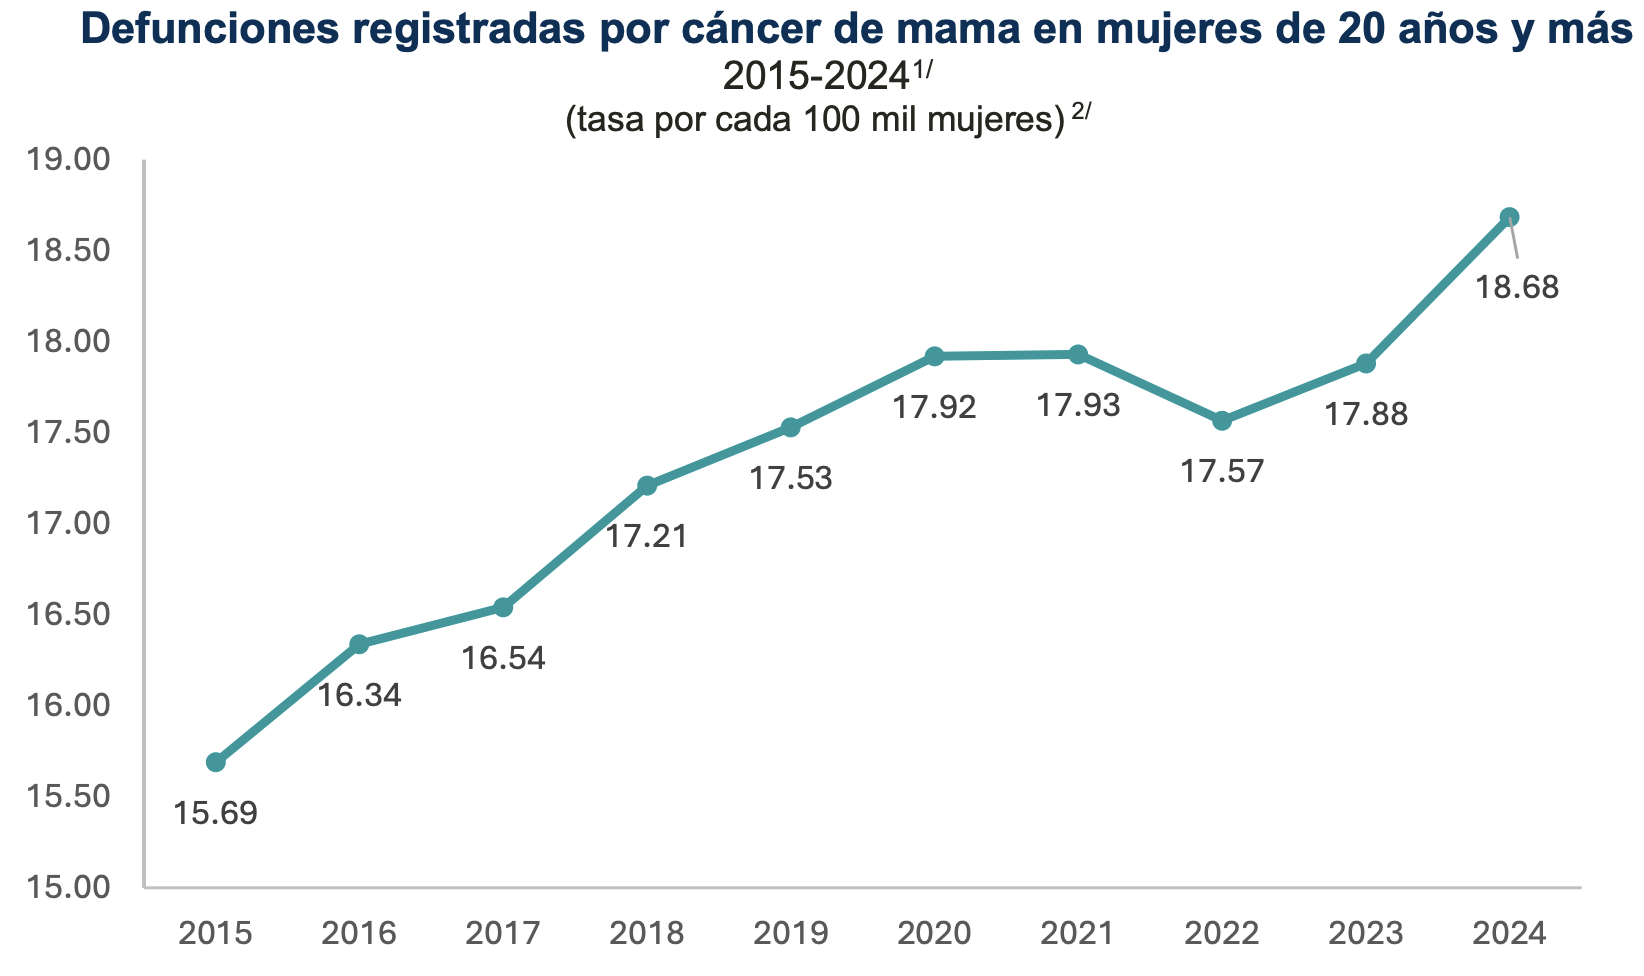
\includegraphics[width=\textwidth]{Figures/Figura_1_1_1.png}
    \caption{Tasa de mortalidad por cáncer de mama en México de 2015 a 2024 \cite{INEGI2025}.}
    \label{fig:MexicoBreastCancerStats}
  \end{subfigure}
  \hfill
  \begin{subfigure}[t]{0.48\textwidth}
    \centering
    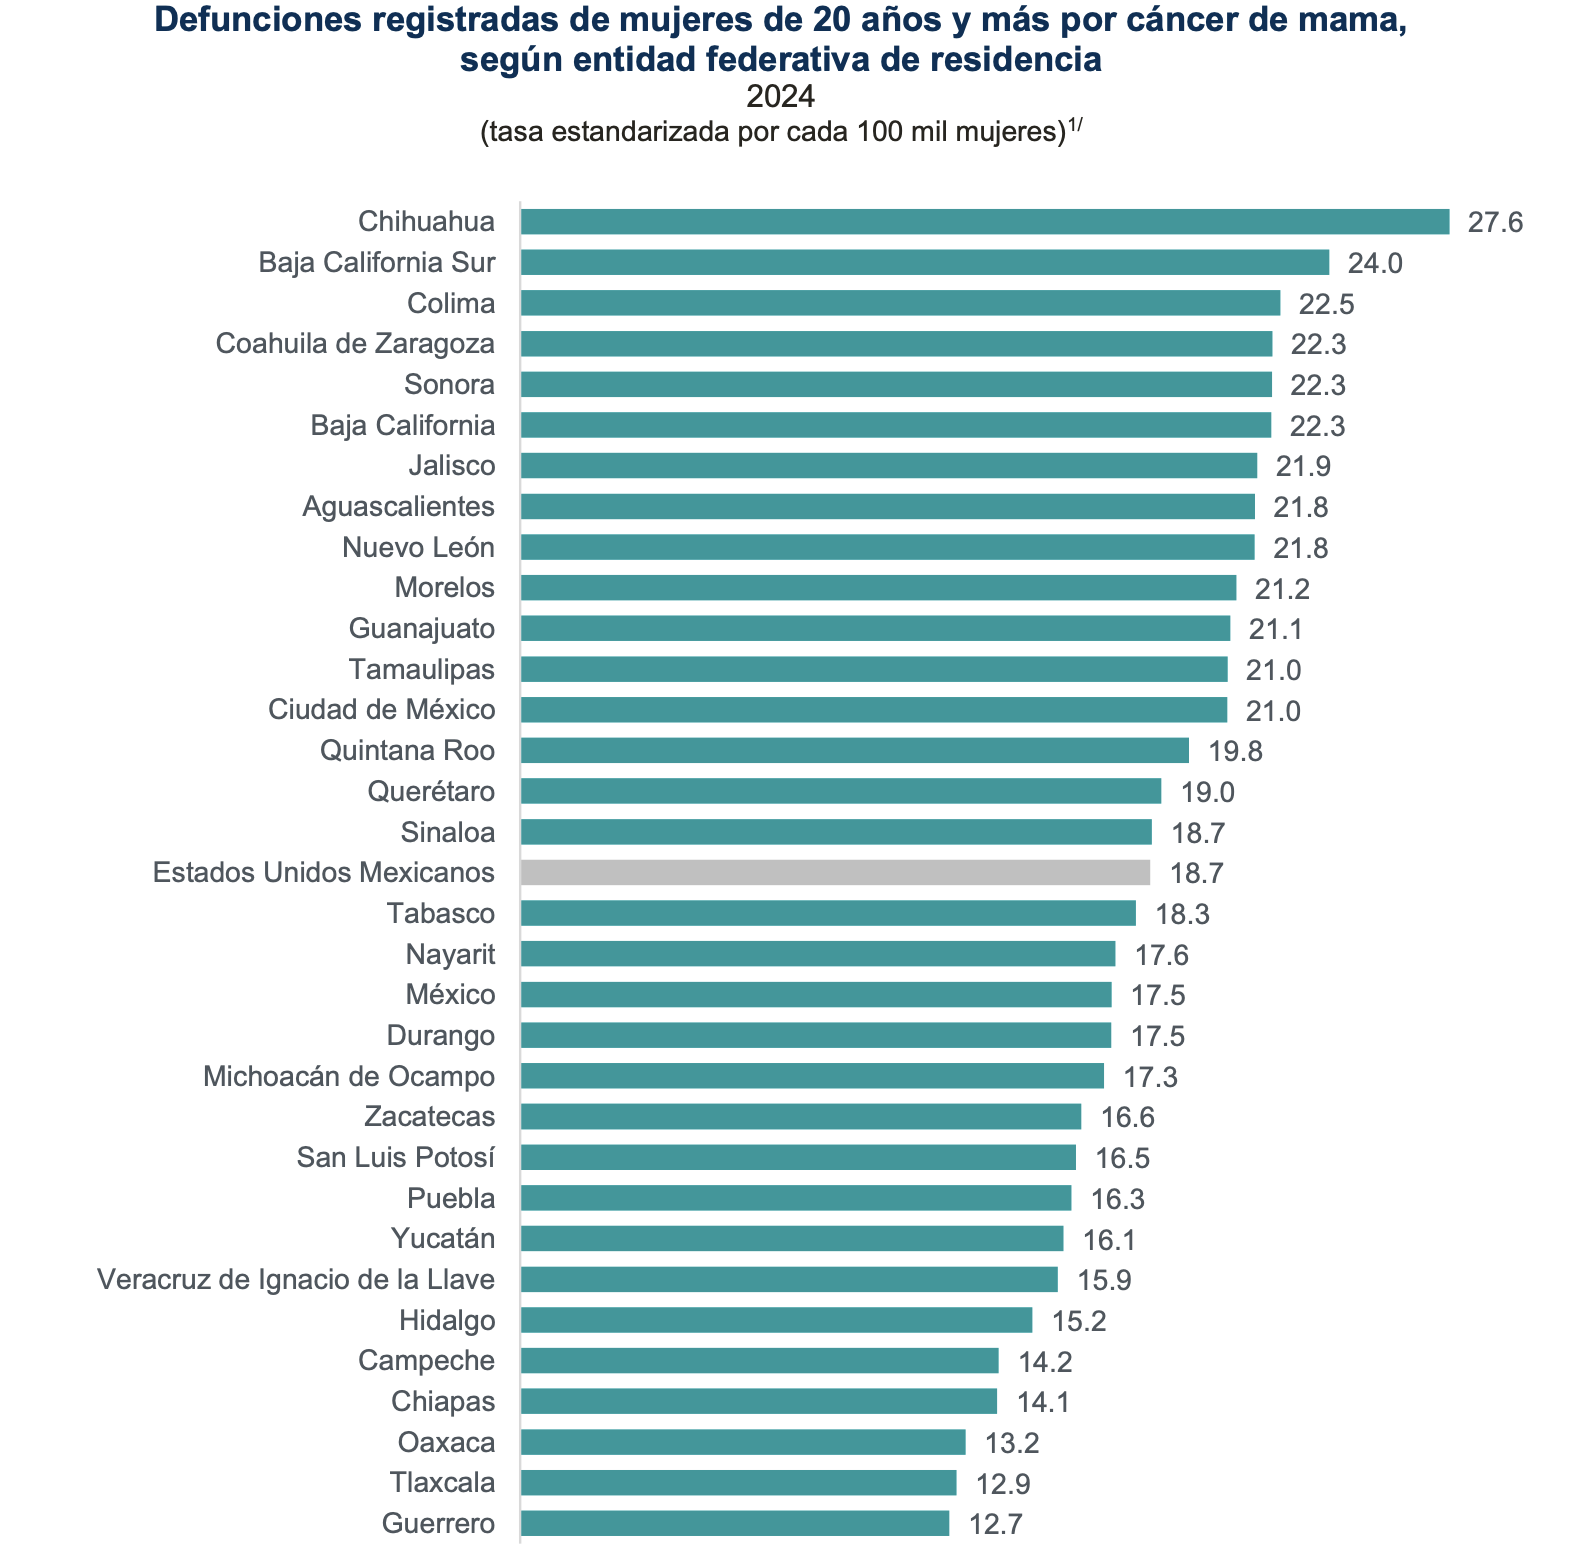
\includegraphics[width=\textwidth]{Figures/Figura_1_1_2.png}
    \caption{Incidencia y mortalidad por entidad federativa en México \cite{INEGI2025}.}
    \label{fig:MexicoBreastCancerStatsByState}
  \end{subfigure}
\end{figure}

\textbf{La detección temprana como factor determinante}

La detección temprana es el factor clínico que más justifica el desarrollo de sistemas de prediagnóstico.
% respaldo: «In fact, according to the American Cancer Society, the 5-year relative survival rate for breast cancer diagnosed at an early, localized stage is over 99%.» (NBCF2026_EarlyDetection, p. 1)
% dato: tabla «Breast Cancer (SEER*) Stage», fila «Distant … 33%» (Docs/fuentes/txt/NBCF2026_Facts/p001.txt, l. 311–313)
Según la American Cancer Society, cuando el cáncer de mama se detecta en una etapa temprana, la supervivencia relativa a cinco años supera el 99\,\%; con metástasis a distancia, según
los datos del programa SEER del National Cancer Institute, es del 33\,\%
\cite{NBCF2026_EarlyDetection, NBCF2026_Facts}.

% respaldo: «Mammography screening has been proven effective in reducing breast cancer deaths in women age 40 years and older. A mortality reduction of 40% is possible with regular screening.» (Monticciolo2021ACR, p. 1)
% respaldo: «radiologists can differ, sometimes substantially, in their interpretations of mammograms and in their recommendations for management.» (Elmore1994, p. 1)
La mamografía es el instrumento central de la detección temprana: el American College of Radiology
señala que el tamizaje mamográfico reduce las muertes por cáncer de mama en mujeres de 40 años o más,
y que con un tamizaje regular es posible una reducción de la mortalidad del 40\,\%
\cite{Monticciolo2021ACR}. Sin embargo, su interpretación manual tiene limitaciones. Los radiólogos
pueden diferir, a veces de forma sustancial, en su interpretación de una misma mamografía y en la
conducta que recomiendan \cite{Elmore1994}; a ello se suman la dificultad de detectar lesiones en tejido
mamario denso y la carga de trabajo creciente de los sistemas de salud. Estos factores
motivan el desarrollo de sistemas de diagnóstico asistido por computadora (CADx).

En México, la infraestructura diagnóstica sigue siendo un desafío. En 2021 se registraron 1\,281
mastógrafos en el país: el 41.1\,\% en instituciones de salud y seguridad social, el 36.1\,\% en
establecimientos particulares y el 22.8\,\% en servicios para población sin derechohabiencia
\cite{INEGI2023}. Esta distribución, junto con el aumento sostenido de la
mortalidad, marca la necesidad de herramientas que amplíen la capacidad diagnóstica del sistema de salud.

En este contexto, el presente trabajo explora el uso de transformaciones cuánticas variacionales
sobre características extraídas de mamografías del dataset CBIS-DDSM, con el fin de evaluar en qué
medida estas representaciones modifican la separación de las clases benigna y maligna cuando se
integran como entrada de una red neuronal clásica.

\subsubsection{Limitaciones de los métodos clásicos de diagnóstico asistido}

El diagnóstico asistido por computadora en mamografía se ha desarrollado notablemente en las últimas
dos décadas, impulsado por las redes neuronales convolucionales (CNN) y el aprendizaje profundo
\cite{TandFOnline2021}. Pese a los resultados reportados en condiciones controladas, estos métodos
presentan limitaciones que restringen su aplicación clínica generalizada.

\textbf{Variabilidad entre conjuntos de datos}

Los modelos de aprendizaje profundo no eliminan la inconsistencia de la interpretación humana: la
trasladan a otro plano. En lugar de variar entre observadores, su desempeño varía entre conjuntos de
% respaldo: «Six deep learning models (three published models with high performance and three models designed by us) were evaluated on four different mammogram data sets» (Wang2020DeepLearning, p. 1)
% respaldo: «However, the same evaluation criteria of all six models on the three external test data sets were significantly decreased, only between 0.44 (95% CI: 0.43-0.45) and 0.65 (95% CI: 0.64-0.66).» (Wang2020DeepLearning, p. 1)
% respaldo: «The three published models reported validation auROC scores between 0.88 and 0.95 on the validation data set.» (Wang2020DeepLearning, p. 1)
datos. Wang et al. \cite{Wang2020DeepLearning} evaluaron seis modelos de aprendizaje profundo, tres
publicados con alto desempeño y tres propios, sobre cuatro conjuntos de mamografías. Los tres modelos
publicados reportaban un AUC-ROC de validación de entre 0.88 y 0.95; sobre los tres conjuntos de
prueba externos, los seis modelos obtuvieron valores de apenas entre 0.44 y 0.65. Un alto desempeño de un sistema CADx en el conjunto de datos con el que se desarrolló no garantiza la
misma efectividad en datos con otra distribución, condición inevitable en la práctica clínica, donde los equipos de adquisición, las
poblaciones y los protocolos de imagen varían.

\textbf{Interpretabilidad}

% Argumento de diseño propio, sin cita (decidido por el autor el 2026-10-16). La cita a Kim et al.
% (2025) de TT1 se retiró: es un artículo epidemiológico que no trata la interpretabilidad (T9 #12).
Una red convolucional profunda aprende sus propias representaciones internas de la imagen, que no
tienen un significado clínico directo. Este trabajo usa, en cambio, características radiómicas, cuyo
significado es explícito: cada una mide una propiedad definida de la intensidad, la textura o la
forma de la lesión. Así es posible saber qué información recibe cada representación y, por tanto,
interpretar qué cambia cuando se le aplica una transformación cuántica.

\textbf{Dimensionalidad y tamaño de los datos}

Las imágenes mamográficas tienen una dimensionalidad muy alta en relación con el número de casos
disponibles. Cuando el conjunto de entrenamiento es pequeño frente al número de parámetros de un
modelo, este tiende a sobreajustarse: aprende los detalles de los datos de entrenamiento y no
generaliza a datos nuevos. El aumento de datos y la regularización mitigan el problema sin
resolverlo, especialmente en conjuntos de tamaño moderado como el CBIS-DDSM.

Estas limitaciones motivan la búsqueda de representaciones alternativas de los datos, entre ellas
las cuánticas, y la evaluación rigurosa de si aportan algo a la separabilidad de las clases.

\subsubsection{Computación cuántica como alternativa}

La computación cuántica ofrece mecanismos distintos para representar y transformar datos. En el
aprendizaje automático, su propuesta no es sustituir a los métodos clásicos, sino intervenir en etapas
específicas del procesamiento, en particular en la codificación de las características.

\textbf{El espacio de Hilbert como espacio de representación}

Un circuito de codificación $U(\mathbf{x})$ define un mapeo no lineal
$\phi: \mathbb{R}^n \rightarrow \mathcal{H}$ que lleva un vector de características clásico
$\mathbf{x}$ a un estado cuántico $|\phi(\mathbf{x})\rangle$ del espacio de Hilbert $\mathcal{H}$. La
geometría de ese espacio la determinan las fidelidades
$|\langle\phi(\mathbf{x})|\phi(\mathbf{x}')\rangle|^2$ entre estados, y no las distancias euclidianas
entre vectores, y depende directamente del diseño del circuito. Cuando el circuito entrelaza los
qubits, la representación puede incorporar dependencias entre pares de características
(sección~\ref{sec:feature_map}). Si esa geometría resulta más favorable para separar lesiones
benignas y malignas que las representaciones clásicas es una pregunta empírica, y es el objeto de
estudio de este trabajo (sección~\ref{sec:planteamiento}).

\textbf{Modelos híbridos cuántico-clásicos para el diagnóstico}

% respaldo: «In this work, we present a quantum hybrid classical convolutional neural network (QCCNN) based breast cancer diagnosis approach with the goal of utilizing quantum computing’s high-dimensional data processing power and parallelism to increase diagnosis efficiency and accuracy.» (Xiang2024QuantumCNN, p. 1)
% respaldo: «The full network is a map from a classical vector space to a classical vector space depending on classical weights.» (Mari2020Transfer, p. 3)
La aplicación del aprendizaje automático cuántico al diagnóstico clínico es una línea de
investigación activa, en la que predominan las arquitecturas híbridas: los circuitos cuánticos se
integran como componentes especializados dentro de un procesamiento mayoritariamente clásico. Xiang
et al. \cite{Xiang2024QuantumCNN} proponen, por ejemplo, una red convolucional híbrida para el
diagnóstico de cáncer de mama con el objetivo de aprovechar el procesamiento de datos de alta
dimensión de la computación cuántica. Mari et al. \cite{Mari2020Transfer} formalizan este tipo de
modelos: la red completa, incluida la capa de codificación cuántica y la medición final, es una
función de un espacio vectorial clásico a otro que depende de pesos clásicos y que, vista desde
fuera, es análoga a una red clásica profunda. Este trabajo usa el circuito de la misma manera, como
una transformación entre representaciones clásicas, pero sin entrenarlo: sus parámetros se fijan para
poder medir su efecto sobre la separabilidad de forma aislada.

\textbf{Estado actual y expectativas}

% respaldo: «We find that overall, out-of-the-box classical machine learning models outperform the quantum classifiers.» (Bowles2024Benchmarking, p. 1)
% respaldo: «Moreover, removing entanglement from a quantum model often results in as good or better performance, suggesting that “quantumness” may not be the crucial ingredient for the small learning tasks considered here.» (Bowles2024Benchmarking, p. 1)
El campo se encuentra en una etapa temprana. En un estudio comparativo a gran escala, Bowles et al.
\cite{Bowles2024Benchmarking} encontraron que, en conjunto, los modelos clásicos estándar, sin ajustes
especiales, superan a los clasificadores cuánticos en las tareas pequeñas que evaluaron, y que eliminar el
entrelazamiento de un modelo cuántico a menudo da un desempeño igual o mejor. Con los dispositivos y
simuladores disponibles no es posible aún demostrar con métricas concluyentes una ventaja de los
modelos cuánticos en problemas prácticos. El valor de una investigación como esta reside en explorar
y documentar, con un protocolo riguroso, sus posibilidades y sus limitaciones en un dominio de alto
impacto como el diagnóstico de cáncer de mama.

% ---
% §1.2 Planteamiento del problema. Reemplaza las líneas 573–603 de Docs/Technical_Report.tex.
% Pregunta de investigación reformulada con el autor el 2026-10-15 (D-041): neutral («modifican»,
% «hasta qué punto»), «características radiómicas» en lugar de «morfológicas» y comparación
% anclada en el mismo vector de características, no en la dimensión.
% Corrige de la auditoría (Docs/insumos/auditoria_s1_s2.md): paráfrasis sin cita de
% Álvarez-Estévez (l. 587 y 591), «geometría euclidiana insuficiente» (refutado por los
% resultados), «caídas de AUC de hasta 0.44 puntos» (Wang et al. reportan AUC de 0.44–0.65,
% no una caída de 0.44) y la presuposición de mejora en la pregunta.
% Decisiones y hallazgos que lo respaldan: D-019, D-031, D-032; H-031, H-039, H-042.
% ---

\subsection{Planteamiento del problema}
\label{sec:planteamiento}

\textbf{La representación como problema}

En el prediagnóstico asistido por computadora, el clasificador no trabaja con la mamografía, sino
con una representación de cada lesión: un vector de descriptores cuantitativos de intensidad,
textura y forma extraídos de la región de interés. La calidad de esa representación limita lo que
cualquier clasificador puede aprender de ella. En el CBIS-DDSM, además, las clases no se distinguen
con la misma facilidad en los dos tipos de hallazgo: en las masas, los descriptores del radiólogo
separan bien las formas irregulares y espiculadas de las ovaladas y circunscritas, mientras que en
las calcificaciones el tipo más frecuente, el pleomórfico, aparece en ambas clases
(capítulo~\ref{sec:eda}). Cabe preguntarse, entonces, si una transformación de esos descriptores
puede reorganizarlos de modo que las lesiones benignas y malignas queden mejor separadas, y si esa
reorganización ayuda a clasificarlas.

\textbf{La propuesta de las codificaciones cuánticas}

Un circuito de codificación $U(\mathbf{x})$ asocia a cada vector de características $\mathbf{x}$ un
estado $|\phi(\mathbf{x})\rangle$ en un espacio de Hilbert de dimensión $2^n$ para $n$ qubits, y la
similitud entre dos lesiones pasa a medirse por la fidelidad
$|\langle\phi(\mathbf{x})|\phi(\mathbf{x}')\rangle|^2$ entre sus estados
(sección~\ref{sec:feature_map}). Los mapas que incluyen compuertas de entrelazamiento, como el
mapa ZZ introducido por Havlíček et al. \cite{havlicek2019supervised}, generan términos que dependen
de pares de características y se han propuesto bajo la conjetura de una posible ventaja cuántica a
corto plazo \cite{AlvarezEstevez2024QuantumKernelBench}. Esa es la motivación de emplearlos como
transformación de los descriptores: no buscar un espacio más grande por sí mismo, sino una geometría
de similitud distinta de la que inducen las transformaciones clásicas.

% respaldo: «If the geometric difference is small, then a classical ML method is guaranteed to provide similar or better performance in prediction on the dataset, independent of the function values or labels.» (huang2021power, p. 2)
% respaldo: «The small geometric difference is a consequence of the exponentially large Hilbert space employed by existing quantum models, where all inputs are too far apart.» (huang2021power, p. 2)
% respaldo: «We show that, under certain conditions, values of quantum kernels over different input data can be exponentially concentrated (in the number of qubits) towards some fixed value.» (Thanasilp2024, p. 1)
% respaldo: «Thus on training with a polynomial number of measurements, one ends up with a trivial model where the predictions on unseen inputs are independent of the input data.» (Thanasilp2024, p. 1)
% respaldo (resumen de arXiv, sin PDF; Docs/fuentes/meta/AlvarezEstevez2024.xml): "However, the practical applicability of these methods remains an open question, particularly beyond the context of specifically-crafted toy problems, and given the current limitations of quantum hardware."
La teoría, sin embargo, no garantiza que esa geometría sea más útil. Huang et al.
\cite{huang2021power} muestran que, si la diferencia geométrica entre un kernel cuántico y los
clásicos es pequeña, un método clásico ofrece un desempeño similar o mejor con cualquier
etiquetado, y observan que en los modelos cuánticos habituales esa diferencia es pequeña porque,
en un espacio de Hilbert exponencialmente grande, todas las entradas quedan demasiado lejos entre
sí. Thanasilp et al. \cite{Thanasilp2024} demuestran que, bajo ciertas condiciones, los valores de
un kernel cuántico se concentran exponencialmente en el número de qubits, de modo que estimarlos
con un número polinomial de mediciones produce un modelo cuyas predicciones no dependen de los
datos. Que una codificación cuántica separe mejor las clases sobre datos clínicos reales es, por
tanto, una pregunta empírica: la aplicabilidad práctica de estos métodos más allá de problemas de
prueba construidos a propósito, y con las limitaciones actuales del \textit{hardware}, sigue
abierta \cite{AlvarezEstevez2024QuantumKernelBench}.

\textbf{La brecha en mamografía}

% respaldo: «In addition, in this research we conduct the experiments using the angle embedding technique since with this method the features can be learned.» (Azevedo2022QuantumTransfer, p. 12)
% respaldo: «As future work, an interesting approach could be to separate the dataset into masses and calcifications and only then perform classification.» (Azevedo2022QuantumTransfer, p. 12)
% respaldo: «Lastly, the best way to know how well this model performs would be to see how the data appears in our Hilbert space. Ideally, both classes would appear very separately in it, as tight clusters.» (Azevedo2022QuantumTransfer, p. 12)
En mamografía, el antecedente más cercano con circuitos cuánticos es el trabajo de Azevedo et al.
\cite{Azevedo2022QuantumTransfer}, que emplean una red híbrida con codificación angular sobre el
BCDR. Entre las líneas que sus autores dejan como trabajo futuro hay dos que este trabajo retoma como ejes: separar masas y
calcificaciones antes de clasificar, y observar cómo se distribuyen los datos en el espacio de
Hilbert, idealmente como conglomerados compactos y separados. La revisión del
capítulo~\ref{sec:antecedentes} no identificó trabajos que evalúen ninguna de las dos sobre el
CBIS-DDSM.

\textbf{La elección del mapa de características}

% respaldo (resumen de arXiv, sin PDF): "Despite outperforming classical methods in ad-hoc datasets, mixed results are obtained for the general case among standard classical benchmarks." / "Instead, it is suggested that a careful choice of the quantum feature map in connection with proper hyperparameterization may prove more effective."
% fuente: D-031
El desempeño de los métodos de kernel cuánticos depende del mapa de características. En una
comparación sobre conjuntos de datos de referencia, Álvarez-Estévez obtiene resultados mixtos
frente a los métodos clásicos y sugiere que una elección cuidadosa del mapa, con una
hiperparametrización adecuada, puede ser más efectiva que optimizar el kernel
\cite{AlvarezEstevez2024QuantumKernelBench}. Este trabajo compara dos mapas que comparten el
acoplamiento ZZ entre pares de características y difieren solo en el eje de la codificación de
primer orden: \textit{ZZFeatureMap}, que gira cada qubit alrededor del eje Z, y
\textit{PauliFeatureMap} con los términos Y y ZZ, que lo gira alrededor del eje Y
(sección~\ref{sec:modulo5}).

\textbf{Formulación del problema de investigación}

A partir de lo anterior, el problema de investigación del presente trabajo se formula de la
siguiente manera:

\begin{quote}
  ¿En qué medida las transformaciones cuánticas variacionales implementadas mediante
  \textit{ZZFeatureMap} y \textit{PauliFeatureMap} en Qiskit modifican la separabilidad de clases
  benigno/maligno de características radiómicas extraídas de mamografías del CBIS-DDSM, y hasta qué
  punto esa diferencia se refleja en la capacidad de clasificación de una misma red neuronal
  clásica, en comparación con representaciones clásicas construidas a partir del mismo vector de
  características?
\end{quote}

La pregunta tiene tres dimensiones, que se abordan de forma integrada. La primera es la de la
representación: si la separabilidad de clases cambia al pasar de las representaciones clásicas a
las cuánticas, medida con métricas geométricas y de kernel (objetivo específico 3). La segunda es
la de la clasificación: si las diferencias de separabilidad se reflejan en el desempeño de un mismo
clasificador y en el orden en que quedan las condiciones (objetivo específico 5). La tercera
acompaña a las dos anteriores y es la de la viabilidad: qué restricciones impone simular estos
circuitos en una computadora clásica y qué implicarían en un procesador cuántico (objetivo
específico 6). La pregunta no presupone el sentido de la respuesta: una separabilidad igual o menor
que la de las representaciones clásicas es también un resultado válido. Los criterios con que se
responde cada dimensión se fijan en el capítulo~\ref{sec:metodologia}.

% ---
% §1.3 Justificación. Reemplaza las líneas 607–631 de Docs/Technical_Report.tex.
% Cambios respecto a TT1 (auditoría T3, §1.3):
%   - \cite de Azevedo et al. (estaba nombrado sin cita) y de Lee et al. / Clark et al. para el CBIS-DDSM;
%   - «circuitos de hasta 16 qubits» → capacidad medida en este trabajo (H-051);
%   - fuera «si demuestran mejorar … clasificadores más generalizables» (presupone el resultado)
%     y «que la literatura menciona pero no sistematiza» (sin fuente);
%   - la relevancia social remite a §1.1 en lugar de repetir cifras;
%   - «datasets predominantes en la literatura» → remite a la tabla comparativa de §2.
% Decisiones y hallazgos que lo respaldan: D-012, D-014, D-019, D-032, D-033; H-051.
% ---

\subsection{Justificación}
\label{sec:justificacion}

\textbf{Relevancia científica}

% respaldo: «Furthermore, results on small datasets cannot be used to reason about larger datasets» (Bowles2024Benchmarking, p. 21)
% respaldo: «There is hence a need to study how results scale to larger datasets, which typically pushes the number of qubits to the limits of what is possible today.» (Bowles2024Benchmarking, p. 22)
El aprendizaje automático cuántico necesita evidencia empírica sobre datos reales. Una parte
importante de su evaluación se ha hecho sobre problemas de prueba construidos para ilustrar
propiedades teóricas \cite{AlvarezEstevez2024QuantumKernelBench}, y los resultados obtenidos con
conjuntos de datos pequeños no permiten razonar sobre conjuntos mayores \cite{Bowles2024Benchmarking}.
Llevar estas técnicas a un dominio de imagen médica, con miles de lesiones y la variabilidad propia de
las mamografías digitalizadas, es la forma de saber cómo se comportan fuera de esas condiciones.

% respaldo: «As future work, an interesting approach could be to separate the dataset into masses and calcifications and only then perform classification.» (Azevedo2022QuantumTransfer, p. 12)
% respaldo: «Lastly, the best way to know how well this model performs would be to see how the data appears in our Hilbert space.» (Azevedo2022QuantumTransfer, p. 12)
El presente trabajo contribuye a esa evidencia de tres formas. Primero, documenta el comportamiento
de \textit{ZZFeatureMap} y \textit{PauliFeatureMap} de Qiskit aplicados a características radiómicas
extraídas de mamografías reales en formato DICOM. Segundo, evalúa las representaciones por su
separabilidad de clases, y no solo por el desempeño del clasificador final, con métricas definidas
sobre los kernels y sobre los propios vectores de representación: el alineamiento kernel-objetivo, la
diferencia geométrica, el índice de Davies-Bouldin y la razón de Fisher (sección~\ref{sec:metricas}).
Tercero, retoma dos de las líneas de trabajo futuro que dejan Azevedo et al.
\cite{Azevedo2022QuantumTransfer}: analizar por separado masas y calcificaciones, y observar cómo se
distribuyen los datos en el espacio de Hilbert. Así, los resultados se sitúan en una línea de
investigación acumulativa en aprendizaje automático cuántico para el diagnóstico médico.

\textbf{Relevancia social}

El cáncer de mama es la principal causa de muerte por tumores malignos en las mujeres de México, y su
detección temprana determina en gran medida el desenlace clínico (sección~\ref{sec:introduccion}).
Las herramientas de prediagnóstico asistido pueden ampliar la capacidad de un sistema de salud en el
que la disponibilidad de mastógrafos y de especialistas en radiología mamaria no cubre la demanda. Para
orientar ese desarrollo es necesario saber qué técnicas aportan y cuáles no: si las representaciones
cuánticas no mejoran la separabilidad de las lesiones, ese resultado, medido con rigor, también indica
dónde no conviene invertir el esfuerzo de investigación. Aunque el presente trabajo es un prototipo
académico y no un dispositivo clínico, sus resultados se suman al conocimiento que eventualmente
informará el desarrollo de herramientas diagnósticas para sistemas de salud con recursos limitados,
como el mexicano.

\textbf{Viabilidad técnica}

% respaldo: «The data were split into a training set and a testing set based on the BI-RADS category.» (Lee2017CBISDDSM, p. 5)
% fuente: D-013, H-032, H-051; B1_benchmark_arquitectura.csv, B1_benchmark_kernel_proyeccion.csv, 8_oe6_qubits.csv, 8_oe6_resumen.csv
% VERIFICAR: licencia CC BY 3.0 del CBIS-DDSM en TCIA (la ficha de Lee no la respalda con cita literal).
La viabilidad del trabajo descansa en tres recursos. El primero es el dataset CBIS-DDSM, una versión
curada del DDSM con diagnóstico confirmado por patología, disponible públicamente en The Cancer
Imaging Archive \cite{Lee2017CBISDDSM, Clark2013TCIA}. En la versión que distribuye TCIA, reúne 3\,568 lesiones de 1\,566 pacientes, con
una partición oficial de entrenamiento y prueba estratificada por categoría BI-RADS y metadatos
clínicos estructurados, lo que evita procesos propios de adquisición, anonimización o validación
clínica. El segundo es la simulación clásica de los circuitos en el equipo de desarrollo, un
procesador Apple M3 con 16 GiB de memoria. El número de qubits se fijó en 12 tras un estudio de
costos: con la implementación inicial, que evaluaba cada valor del kernel con un circuito propio, la
etapa cuántica completa pasaba de unas 3~h con 12 qubits a unas 41~h con 16, y el diseño requiere
decenas de kernels. Después se adoptó una implementación que calcula el vector de estado de cada
lesión una sola vez y obtiene el kernel de sus productos internos; con ella se comprobó que el límite
físico de la máquina está más arriba, pues se simularon estados de hasta 28 qubits
(sección~\ref{sec:resultados}). Estas cifras corresponden a la simulación ideal del vector de estado,
sin ruido, que además permite aislar el efecto de la transformación cuántica sin la interferencia del
ruido de los dispositivos físicos. El tercero es un ecosistema de
programación de código abierto, documentado y mantenido (Qiskit, PyTorch, PyRadiomics, scikit-learn),
que permite a otros investigadores reproducir el trabajo.

\textbf{Novedad y posicionamiento frente a trabajos previos}

La aportación del trabajo se define por tres diferenciadores. El primero es el dominio de datos:
opera sobre mamografías DICOM del CBIS-DDSM y no sobre datos clínicos tabulares, como Wisconsin, SEER o
GBSG, empleados en otros trabajos de aprendizaje automático cuántico en oncología
(cuadro~\ref{tab:estado_arte_v2}). El segundo es el papel del componente cuántico: el circuito se usa
exclusivamente como transformación de la representación, con parámetros fijos, y no como una capa que
se entrena dentro de una red, lo que permite analizar de forma aislada su efecto sobre la
separabilidad de las clases. El tercero es el análisis de viabilidad: las restricciones prácticas del
simulador se convierten en un objetivo de investigación explícito y medible, con datos cuantitativos
sobre el tiempo de ejecución, el número de qubits simulables, el número de mediciones que requeriría
un procesador real y el costo de entrenar el circuito. En conjunto, estos diferenciadores sitúan el
trabajo como una contribución experimental a una línea de investigación activa y como una referencia
metodológica para aplicar codificaciones cuánticas a la imagen médica.

% ---
% §1.4 Objetivos. Reemplaza las líneas 635–658 de Docs/Technical_Report.tex.
% Cambio mínimo respecto al protocolo de TT1, registrado en D-041 (Other/bitacora_decisiones.md),
% pendiente de confirmar con los directores. Cambios:
%   OG   «capacidad … para generar espacios con mayor separabilidad» → «efecto … en la separabilidad»;
%        «morfológicas» → «radiómicas»; «kernel RBF clásico» → «kernels clásicos de referencia» (D-032);
%        «la mejora … se traduce en una mejora» → «las diferencias … se reflejan»;
%        «distancia Fisher» → «razón de Fisher» (D-033).
%   OE-1 sin «normalización» ni «encoder CNN preentrenado» (D-006, D-009, D-010); recorte a resolución original.
%   OE-2 C4 y C5 con capa variacional de parámetros fijos (D-014); C5 con términos Y y ZZ (D-031).
%   OE-3 geometric difference frente a kernels clásicos de referencia, sin «estructura inaccesible» (D-032).
%   OE-5 «la mejora … se traduce» → «las diferencias … se reflejan»; «ranking» → «ordenamiento».
%   OE-6 redacción («Evaluar o analizar» → «Analizar») y número de mediciones en un procesador real (D-040).
% ---

\subsection{Objetivos}
\label{sec:objetivos}

\subsubsection{Objetivo general}

Analizar el efecto de las transformaciones cuánticas variacionales implementadas mediante
\textit{ZZFeatureMap} y \textit{PauliFeatureMap} en Qiskit, sobre características radiómicas
extraídas de imágenes mamográficas del dataset CBIS-DDSM, en la separabilidad de clases
benigno/maligno, cuantificando dicha separabilidad mediante \textit{kernel-target alignment},
\textit{geometric difference} respecto a kernels clásicos de referencia, índice de Davies-Bouldin y
razón de Fisher, comparando contra representaciones clásicas de referencia (sin transformación, PCA
lineal y Kernel PCA con kernel RBF) construidas a partir del mismo vector de características
seleccionadas y escaladas, e integrando todas las representaciones resultantes como entrada de un
mismo clasificador MLP para determinar si las diferencias en separabilidad se reflejan en la
capacidad de clasificación binaria.

\subsubsection{Objetivos específicos}

\begin{enumerate}
  \item Construir un \textit{pipeline} de preprocesamiento sobre el dataset CBIS-DDSM que comprenda
  la lectura de imágenes en formato DICOM, el recorte de la región de interés (ROI) a resolución
  original, la extracción de un vector de características radiómicas mediante PyRadiomics y la
  selección de las $k$ características más discriminativas mediante SelectKBest con escalado
  angular al rango $[0,\pi]$, diferenciando el procesamiento de casos de masas y calcificaciones
  como subproblemas independientes.
  \item Implementar las cinco condiciones de transformación del experimento sobre el mismo vector
  de entrada: (a) sin transformación, como referencia sin procesar; (b) PCA lineal, como referencia
  lineal; (c) Kernel PCA con kernel RBF, como referencia no lineal; (d) circuito cuántico
  variacional con \textit{ZZFeatureMap}, implementado en Qiskit Aer con una capa variacional
  RealAmplitudes de parámetros fijos; y (e) circuito cuántico variacional con
  \textit{PauliFeatureMap} con los términos Y y ZZ, con la misma capa variacional, asegurando que
  todas las condiciones produzcan vectores de representación de dimensión $k$ como entrada al
  clasificador MLP.
  \item Analizar y comparar la separabilidad de clases benigno/maligno en los espacios de
  representación generados por las cinco condiciones experimentales mediante: \textit{kernel-target
  alignment} (KTA) respecto al kernel ideal de clasificación; \textit{geometric difference} entre el
  kernel cuántico y un conjunto de kernels clásicos de referencia, como indicador de si el espacio
  cuántico induce una geometría que los métodos clásicos no reproducen; índice de Davies-Bouldin,
  como medida de compacidad y separación de los grupos; y razón de Fisher, como cociente de la
  dispersión entre clases sobre la dispersión dentro de cada clase; aplicando el análisis de forma
  independiente para masas y calcificaciones.
  \item Entrenar un mismo clasificador MLP sobre cada uno de los cinco vectores de representación
  generados en el objetivo específico 2, manteniendo idéntica arquitectura, hiperparámetros y
  protocolo de entrenamiento en todas las condiciones.
  \item Evaluar si las diferencias de separabilidad observadas en el objetivo específico 3 se
  reflejan en la capacidad de clasificación binaria, comparando las métricas AUC-ROC, F1-Score,
  Accuracy, Precision y Recall obtenidas por el MLP en las cinco condiciones y analizando la
  correlación entre el ordenamiento de separabilidad y el de clasificación, con todos los resultados
  reportados por separado para masas y calcificaciones del CBIS-DDSM.
  \item Analizar los beneficios y las limitaciones prácticas, incluidas las restricciones
  computacionales del simulador cuántico y el número de mediciones que requeriría un procesador
  real, para valorar la viabilidad de aplicar estas técnicas en un contexto de salud.
\end{enumerate}

% ---
% §1.5 Alcance y limitaciones. Reemplaza las líneas 662–688 de Docs/Technical_Report.tex.
% Cambios respecto a TT1:
%   - propósito y pregunta alineados con la pregunta reformulada (§1.2, D-041);
%   - se añaden las codificaciones evaluadas y excluidas (decidido con el autor el 2026-10-15)
%     y las limitaciones de datos y de diseño;
%   - se quitan la analogía del ENIAC y el párrafo de Grover (auditoría T3: fuera de tema y sin
%     cita; la afirmación sobre NISQ y Grover no tenía fuente). El texto original sigue en el .tex.
% Decisiones y hallazgos que lo respaldan: D-005, D-013, D-014, D-031; H-002, H-035, H-045, H-051,
% H-052, H-054.
% ---

\subsection{Alcance y limitaciones}
\label{sec:alcance}

El presente trabajo tiene como propósito central evaluar la viabilidad de las transformaciones
cuánticas variacionales como mecanismo de codificación de características radiómicas extraídas de
imágenes mamográficas, determinando en qué medida modifican la separabilidad de clases
benigno/maligno frente a representaciones clásicas construidas a partir del mismo vector de
características. El sistema desarrollado constituye un prototipo de investigación académica, no un
sistema de diagnóstico clínico, y su alcance está delimitado por los criterios siguientes.

\textbf{Datos y tarea}

El sistema opera exclusivamente sobre las lesiones del dataset CBIS-DDSM que corresponden a masas y
calcificaciones con diagnóstico patológico confirmado, a partir de la región de interés que delimita
la máscara de cada lesión. Masas y calcificaciones se tratan como subproblemas independientes en
todo el \textit{pipeline}. El problema abordado es la clasificación binaria benigno/maligno; la
detección de lesiones, su localización espacial y la segmentación quedan fuera del alcance.

\textbf{Simulación clásica}

% respaldo: «“Noisy” emphasizes that we’ll have imperfect control over those qubits; the noise will place serious limitations on what quantum devices can achieve in the near term.» (Preskill2018NISQ, p. 5)
La totalidad de los experimentos cuánticos se ejecuta en simulación clásica con Qiskit Aer, sin
acceso a \textit{hardware} cuántico. Los resultados corresponden, por tanto, a condiciones ideales,
libres del ruido de los dispositivos físicos, lo cual es una condición deliberada del diseño
experimental y no una deficiencia metodológica: permite atribuir lo observado a la codificación y no
al ruido. Los dispositivos actuales, de escala intermedia y con ruido (NISQ), tienen un control
imperfecto de sus qubits, y ese ruido limita lo que pueden lograr a corto plazo
\cite{Preskill2018NISQ}. Lo que este trabajo dice sobre la ejecución en un procesador real se basa en
proyecciones: el número de mediciones se estudia con un muestreo ideal de las probabilidades
exactas, sin modelar el ruido del dispositivo.

\textbf{Codificaciones evaluadas}

El estudio se limita a dos mapas de características con entrelazamiento entre todos los pares de
qubits, \textit{ZZFeatureMap} y \textit{PauliFeatureMap} con los términos Y y ZZ, con una repetición
y $k = 12$ qubits. El número de qubits se fijó por el costo de simulación y por la diversidad de
familias de características que conserva la selección, y obliga a descartar parte de la información
de las 67 características extraídas. Quedan fuera las codificaciones sin entrelazamiento, como la
angular producto o la codificación en amplitudes, porque su kernel es por construcción un kernel
clásico (sección~\ref{sec:modulo5}). Los parámetros de la capa variacional se fijan con una semilla
y no se entrenan, para que la separabilidad se mida sobre una representación no supervisada;
entrenarlos se explora solo como experimento complementario.

\textbf{Datos de imagen}

Las mamografías del CBIS-DDSM son películas digitalizadas sin escala física de intensidad ni
espaciado de píxel en sus metadatos, de modo que las características de primer orden se calculan
sobre intensidades no calibradas y las de forma se expresan en píxeles. Todos los resultados
provienen de un único conjunto de datos, sin validación externa, y el conjunto de prueba oficial se
usa una sola vez por modelo.

\textbf{El objetivo no es superar lo existente, sino explorar lo posible}

Un error frecuente en la evaluación de trabajos de aprendizaje automático cuántico aplicado consiste
en juzgar su validez en función de si el modelo cuántico supera en precisión a los mejores modelos
clásicos disponibles. Este criterio, pertinente para tecnologías maduras, resulta inapropiado para el
estado actual de la computación cuántica. El objetivo del presente trabajo no es demostrar que las
representaciones cuánticas superan a una CNN de última generación en AUC-ROC, sino responder la
pregunta planteada en la sección~\ref{sec:planteamiento}: en qué medida estas transformaciones
modifican la separabilidad intrínseca de las clases sobre datos mamográficos reales, y si esa
diferencia se refleja en la clasificación. Una mejora en separabilidad sin mejora en la clasificación
constituiría evidencia válida sobre el comportamiento de estos circuitos, y también lo es una
separabilidad igual o menor que la clásica, siempre que esté medida con el mismo rigor y que se
documenten las restricciones que la explican.

\newpage

% ===== Capítulo: 2_Antecedentes
\setcounter{section}{1}
% ---
% Reemplaza líneas 692–700 de Docs/Technical_Report.tex.
% Copia literal de TT1; pendiente de corrección con Docs/insumos/auditoria_s1_s2.md.
% ---

\section{Antecedentes}
\label{sec:antecedentes}
% -----------------------------------------------------------
% 2.1 Estado del arte
% -----------------------------------------------------------
\subsection{Estado del arte}

% -----------------------------------------------------------
% 2.1.1 ML Clásico en diagnóstico de cáncer de mama
% -----------------------------------------------------------

% ---
% Reemplaza líneas 701–725 de Docs/Technical_Report.tex.
% Reescrito en TT2 con Docs/insumos/auditoria_s1_s2.md y las fichas de T10:
% - las razones de la preferencia por SVM no están en Mashekova et al.; se quitan de la atribución;
% - en Añez et al., SVM y XGBoost reciben solo cuatro rasgos globales de la imagen completa;
% - sin presuponer que las características diseñadas por expertos son insuficientes (las radiómicas
%   con un clasificador clásico son la referencia más fuerte del proyecto, H-042, H-044).
% PENDIENTE: el párrafo sobre GLCM y descriptores de forma depende de Zebari et al. (TandFOnline2021),
% que es de acceso abierto pero no se pudo descargar de forma automática (informe T10).
% Cada atribución lleva su respaldo verificable con Code/tools/verificar_citas_fichas.py.
% ---

\subsubsection{Aprendizaje automático clásico en el diagnóstico mamográfico}

Los sistemas de detección y diagnóstico asistidos por computadora (CAD, \textit{Computer-Aided Detection/Diagnosis}) en mamografía buscan apoyar la interpretación radiológica y la detección temprana de lesiones. Los sistemas clásicos se organizan en dos etapas: la extracción de características diseñadas a partir de la imagen y su clasificación con un algoritmo de aprendizaje supervisado.

\textbf{Extracción de características}

% VERIFICAR con Zebari et al. (TandFOnline2021) cuando se tenga el PDF: que GLCM es la técnica de
% extracción más usada en los trabajos que revisan, y los descriptores de forma, margen y distribución.
Entre las características más usadas están las de textura derivadas de la matriz de co-ocurrencia de niveles de gris (GLCM) \cite{TandFOnline2021}, junto con descriptores de forma y margen para las masas y de distribución espacial para las calcificaciones.
% respaldo: «In this study, Gray Level Co-occurrence Matrix (GLCM) and Gray Level Run Length Matrix (GLRLM) features, which are widely used in texture analysis, were extracted from each ROI sample.» (Avci2023MammographyEnhancement, p. 6)
Las matrices GLCM y GLRLM (\textit{Gray Level Run Length Matrix}) son de uso extendido en el análisis de textura \cite{Avci2023MammographyEnhancement}, y son dos de las familias de características que este trabajo extrae con PyRadiomics.

\textbf{Clasificadores}

% respaldo: «The analysis of the abovementioned databases demonstrates that approximately 44% of the studies published between 2020 and 2025 employed support vector machine (SVM) as a classifier for breast cancer detection.» (Mashekova2025AIBreastCancer, p. 14)
% respaldo: «SVM was most frequently associated with mammogram images, although some studies also utilized ultrasound and, to a lesser extent, thermography images.» (Mashekova2025AIBreastCancer, p. 14)
La máquina de vectores de soporte (SVM) es el clasificador clásico más usado en este dominio: según la revisión de Mashekova et al., cerca del 44~\% de los estudios publicados entre 2020 y 2025 sobre detección de cáncer de mama la emplearon, sobre todo con mamografías \cite{Mashekova2025AIBreastCancer}.
% respaldo: «These approaches heavily rely on handcrafted features, which limit generalizability but allow transparency and interpretability.» (Mashekova2025AIBreastCancer, p. 26)
Los mismos autores señalan que estos métodos dependen de características diseñadas a mano, lo que limita su generalización pero los hace transparentes e interpretables \cite{Mashekova2025AIBreastCancer}.

% respaldo: «In our study, SVM, RF, and ANN methods generally performed better than k-NN, NB, and DT especially in CLAHE&USM, and MF&CLAHE&USM pre-processing combinations.» (Avci2023MammographyEnhancement, p. 11)
% respaldo: «When the CLAHE algorithm is used alone as a pre-processing method, it has been observed that it has a lower classification performance than other pre-processing combinations.» (Avci2023MammographyEnhancement, p. 12)
% respaldo: «The open-access mini-MIAS database was used in the study [16].» (Avci2023MammographyEnhancement, p. 4)
Avcı y Karakaya compararon SVM, bosques aleatorios (RF), redes neuronales (ANN), $k$ vecinos más cercanos, Naive Bayes y árboles de decisión sobre características GLCM y GLRLM de la base mini-MIAS. SVM, RF y ANN rindieron en general mejor que el resto, y el desempeño dependió de la combinación de preprocesamiento aplicada antes de extraer las características \cite{Avci2023MammographyEnhancement}.

\textbf{Alcances y limitaciones}

% respaldo: «The best CNN (ResNet-50) achieved an AUC-ROC of 0.95 with a Recall of 89%, while the XGBoost model reached an AUC-ROC of 0.90 with a Recall of 74%,» (Anez2025AIPipeline, p. 27)
% respaldo: «followed by XGBoost (AUC-ROC 0.90; sensitivity 74%) and SVM (AUC-ROC 0.84; sensitivity 66%)» (Anez2025AIPipeline, p. 1)
% respaldo: «These models were trained on handcrafted features extracted directly from full mammographic images, including mean intensity, standard deviation, width, and height.» (Anez2025AIPipeline, p. 10)
Las comparaciones entre enfoques dependen de lo que recibe cada clasificador. En la evaluación de Añez et al. sobre el CBIS-DDSM, una ResNet-50 alcanzó un AUC-ROC de 0.95, frente a 0.90 de XGBoost y 0.84 de una SVM \cite{Anez2025AIPipeline}; pero los dos modelos clásicos recibieron solo rasgos globales de la mamografía completa, como la intensidad media, su desviación, el ancho y el alto \cite{Anez2025AIPipeline}. La diferencia mide, sobre todo, la distancia entre esos rasgos y lo que la red aprende de los píxeles.

La capacidad discriminativa de un clasificador clásico está acotada por la información que contienen las características que recibe. Esa limitación motivó los enfoques de aprendizaje profundo, que aprenden la representación desde los píxeles (sección siguiente), y más tarde el interés por las representaciones cuánticas. Pero las características radiómicas siguen siendo una referencia exigente: en el presente trabajo, las mismas características con un clasificador clásico son la condición contra la que se comparan las transformaciones cuánticas.

% ---
% Reemplaza líneas 726–750 de Docs/Technical_Report.tex.
% Copia literal de TT1; pendiente de corrección con Docs/insumos/auditoria_s1_s2.md.
% ---

\subsubsection{Deep Learning en el diagnóstico mamográfico}

\textbf{El avance de las CNN en mamografías}

La aplicación de redes neuronales convolucionales (CNN) en el análisis de mamografías marcó un nuevo paradignma respecto a los sistemas CAD clásicos. A diferencia de los enfoques basados en features manuales, las CNN aprenden representaciones jerárquicas directamente desde los píxeles de la imagen, eliminando la dependencia de descriptores diseñados por expertos. Las CNN poco profundas fueron utilizadas para investigar el cáncer de mama desde 1995; sin embargo, fue a partir de 2012, con el surgimiento de Alex-Net y el aumento de la capacidad computacional, la disponibilidad de hardware de menor costo, los algoritmos de código abierto y el auge del big data, cuando las CNN se volvieron predominantes en el procesamiento de imágenes médicas. Arquitecturas como VGG, ResNet, DenseNet e InceptionV3 se convirtieron en la base de la mayoría de los sistemas CAD modernos para mamografía. \cite{Abdelhafiz2019DeepCNN}

\textbf{Resultados reportados en distintos datasets}

Los modelos de deep learning han alcanzado resultados notables en condiciones controladas sobre los datasets más utilizados en la comunidad. Shen et. al \cite{Shen2019DeepLearning} desarrollaron un sistema de CNN de extremo a extremo sobre CBIS-DDSM con un enfoque que aprovecha tanto anotaciones de lesiones como etiquetas de imagen completa, el mejor modelo individual alcanzó un AUC por imagen de 0.88 sobre el conjunto de prueba del CBIS-DDSM, y el promedio de cuatro modelos mejoró este resultado a un AUC de 0.91, con una especificidad de 80.1\% a una sensibilidad de 86.1\%, comparable al promedio estimado de radiólogos en Estados Unidos.

En el dominio específico de las calcificaciones, la comparación entre arquitecturas evidencia diferencias significativas según el tipo de lesión. Al evaluar modelos ResNet-50, ResNet-101 y cinco variantes de EfficientNet (B0 a B4) para clasificación de microcalcificaciones benignas y malignas usando validación cruzada de cinco pliegues sobre imágenes mamográficas con etiquetas BI-RADS confirmadas, todos los modelos EfficientNet superaron significativamente a las variantes ResNet en F1-score; adicionalmente, bajo validación externa con CBIS-DDSM, EfficientNet-B3 mantuvo su superioridad con mayor recall tanto para clases benignas como malignas. Este hallazgo nos muestra que el performace de un modelo es sensible no solo al dataset de entrenamiento sino al tipo de hallazgo mamográfico analizado, lo que refuerza la necesidad de evaluar masas y calcificaciones de forma separada. \cite{Shia2025MicrocalcClassification}

\textbf{El problema de la generalización}

A pesar de los resultados prometedores reportados en validación interna, existe un problema estructural que la literatura ha mencionado de manera consistente, los modelos de deep learning no generalizan entre datasets con distribuciones distintas. Wang et al. (2020) realizaron el análisis más sistemático de este fenómeno, evaluando seis modelos sobre cuatro datasets diferentes. Como se señaló en la sección 1.1.2, los modelos que reportaron AUC de validación entre 0.88 y 0.95 mostraron caídas hasta el rango de 0.44--0.65 al evaluarse sobre datos externos. La variabilidad entre lectores y la dificultad intrínseca de interpretar características radiográficas sutiles limitan frecuentemente la precisión del diagnóstico; el impacto del cambio de dominio queda evidenciado en pruebas de generalización, que marcan la necesidad de conjuntos de datos diversos durante el entrenamiento para construir herramientas de tamizaje confiables y ampliamente aplicables.

Este problema tiene raíces más profundas que la simple escasez de datos. La investigación futura debe enfocarse en enriquecer los algoritmos de deep learning, garantizar la privacidad de los datos, mejorar la interpretabilidad de los modelos y establecer la generalización para integrar exitosamente el diagnóstico asistido por deep learning en programas rutinarios de tamizaje de cáncer de mama.

\textbf{La representación como problema central}

El análisis de la literatura permite identificar que el problema no es la arquitectura del clasificador sino la calidad de la representación que este recibe. Los modelos de deep learning operan en el espacio de píxeles o en espacios de features aprendidos mediante backpropagation, cuya geometría está determinada por la función de pérdida de clasificación y el conjunto de entrenamiento disponible. Esta representación puede ser altamente efectiva dentro del dominio de entrenamiento pero frágil ante cambios de distribución. La pregunta que motiva el presente trabajo es si la proyección de estas características al espacio de Hilbert mediante transformaciones cuánticas variacionales puede generar representaciones con mayor separabilidad intrínseca de clases, abordando el problema desde la etapa de codificación y no desde la arquitectura del clasificador.

% -----------------------------------------------------------
% 2.1.3 Fundamentos de QML y codificación cuántica de datos
% -----------------------------------------------------------

% ---
% Reemplaza líneas 751–798 de Docs/Technical_Report.tex.
% Copia literal de TT1; pendiente de corrección con Docs/insumos/auditoria_s1_s2.md.
% ---

\subsubsection{Fundamentos de quantum machine learning y codificación cuántica de datos}

\textbf{El origen teórico, QML como extensión de kernerls}

El quantum machine learning (QML) surge de una observación fundamental establecida por Schuld y Killoran en 2019, la idea básica de la computación cuántica es sorprendentemente similar a la de los métodos kernel en machine learning, es decir, realizar eficientemente cómputos en un espacio de Hilbert de tamaño intratable. El proceso de codificar entradas en un estado cuántico se interpreta como un mapa de características no lineal que mapea datos al espacio de Hilbert cuántico; en este espacio de características, el dispositivo cuántico puede estimar productos internos de estados cuánticos para computar un kernel clásicamente intratable, el cual puede alimentar cualquier modelo clásico como una máquina de vectores de soporte.
Esta formalización sentó las bases teóricas de todo el campo del QML moderno y es la justificación fundamental del presente trabajo: si el espacio de Hilbert de $2^n$ dimensiones generado por $n$ qubits ofrece una geometría más favorable para la separación de clases morfológicas mamográficas, entonces la proyección cuántica aporta valor real al pipeline de clasificación. \cite{Schuld2019QuantumML}

El trabajo de Havlíček et al. (2019) en IBM Nature formalizó esta idea operacionalmente, demostrando dos algoritmos de clasificación que usan el espacio de estados cuánticos para producir mapas de características, probados en procesadores superconductores. Esto estableció el ZZFeatureMap como referencia estándar en la comunidad y demostró la posibilidad de ventaja cuántica cuando el espacio de características es grande y las funciones kernel son computacionalmente costosas de estimar clásicamente.

\textbf{Circuitos cuánticos variacionales}

Los circuitos cuánticos variacionales (VQC) son la arquitectura predominante en QML para el régimen NISQ actual. Los VQC son un tipo específico de circuito cuántico parametrizado (PQC) que combina circuitos cuánticos con optimizadores clásicos; son ampliamente utilizados en algoritmos cuánticos y, entre los distintos tipos de PQC, son el enfoque que típicamente optimiza sus parámetros mediante métodos variacionales, minimizando una función de costo mediante optimización híbrida cuántico-clásica. \cite{Long2025HybridQCQ}

Un VQC está estructurado en tres bloques consecutivos que corresponden directamente a la arquitectura a implementar en el presente trabajo. El primero es el mapa de características $U(x)$, que codifica el vector clásico $x$ en el estado cuántico inicial $|\phi(x)\rangle = U(x)|0\rangle^{\otimes n}$. El segundo es el ansatz variacional $W(\theta)$, que aplica rotaciones parametrizadas y compuertas de entrelazamiento entrenables, generando el estado final $|\psi(x,\theta)\rangle = W(\theta)|\phi(x)\rangle$. El tercero es la medición, que extrae el vector de valores de expectativa $\langle Z_i \rangle$ de cada qubit como salida clásica del circuito.

Los parámetros $\theta$ se optimizan mediante el método de
parameter-shift, que calcula el gradiente exacto del circuito evaluándolo en dos puntos desplazados: $\nabla_\theta \langle O \rangle = \frac{1}{2}[\langle O \rangle_{\theta+\pi/2} - \langle O \rangle_{\theta-\pi/2}]$.
Este método es diferenciable durante el proceso de entrenamiento y compatible con backpropagation clásico, lo que habilita el entrenamiento conjunto del circuito cuántico y la red neuronal clásica downstream mediante optimizadores estándar de PyTorch.

\textbf{Los métodos de codificación cuántica}

La elección del método de codificación es la decisión de diseño más importante en un sistema QML, ya que determina la geometría del espacio de Hilbert donde los datos quedan representados. La integración de técnicas de codificación cuántica de datos en algoritmos de machine learning clásicos contribuye a mejorar la precisión de clasificación y los valores F1, de manera particularmente notable en modelos que se benefician intrínsecamente de una representación de características enriquecida.

Los tres tipos de codifiacación más utilizados en la literatura son:

\begin{itemize}
  \item \textbf{Angle encoding}: codifica cada componente del vector de características como un ángulo de rotación en un qubit, por ejemplo, $x_i$ se codifica como una rotación $R_y(x_i)$ en el qubit $i$. Es simple pero puede requerir muchos qubits para vectores de alta dimensionalidad. Su principal ventaja es la simplicidad y la diferenciabilidad directa; su limitación es que las relaciones entre características solo se pueden expresar a través de las capas variacionales posteriores, no en la etapa de codificación.
  \item \textbf{ZZFeatureMap}: construido sobre el mapa angular, agrega compuertas de entrelazamiento entre pares de qubits que codifican productos de features: $e^{i x_i x_j Z_i Z_j}$. El ZZFeatureMap captura interacciones de features por pares, pero algunos datasets requieren interacciones de orden superior.
  \item \textbf{PauliFeatureMap}: generaliza el ZZFeatureMap agregando rotaciones alrededor de los tres ejes de Pauli $(X, Y, Z)$ y operaciones de entrelazamiento más complejas. El PauliFeatureMap extiende la codificación utilizando rotaciones multi-eje y entrelazamiento cuántico complejo para codificar dependencias de características más profundas; es altamente expresivo, capaz de capturar interacciones de orden superior y patrones ocultos dentro de los datos, siendo particularmente poderoso para datasets donde las relaciones entre características son complejas y no lineales. Su mayor expresividad tiene como contrapartida una mayor sensibilidad al ruido cuántico, relevante incluso en simulación cuando el número de shots es limitado.

\end{itemize}

La elección entre estos métodos de codificación no es trivial y depende de la estructura de correlación de los datos de entrada. Un estudio reciente aplicó los tres métodos a la clasificación de cáncer de pulmón con QSVM, obteniendo que ZZFeatureMap alcanzó una accuracy de 0.91 y F1-score de 0.91, mientras que PauliFeatureMap logró un rendimiento consistente de 0.96 en todas las métricas incluyendo accuracy, precisión, recall y F1-score; la elección del mapa apropiado depende de dos factores principales, la naturaleza de los datos y la resiliencia al ruido del dispositivo cuántico. Estos resultados motivan la estrategia del presente trabajo de comparar ambos métodos de codifiación sobre características morfológicas mamográficas.


\textbf{El problema "barren plateau"}

Una limitación teórica importante de los VQC profundos es el fenómeno del *barren plateau*. A medida que el circuito aumenta en número de qubits y capas, la optimización se vuelve exponencialmente plana, con gradientes que convergen a cero. Esto hace el entrenamiento prácticamente imposible para circuitos de gran profundidad con una inicialización aleatoria de parámetros. 
Esta limitación tiene implicaciones directas para el diseño del experimento, justifica el uso de circuitos de profundidad moderada y la estrategia de inicialización cuidadosa de los parámetros $\theta$.

\textbf{El uso de Qiskit como plataforma de desarrollo}

Qiskit, es el framework de código abierto de IBM para computación cuántica, provee la infraestructura completa para implementar el pipeline descrito. Su ecosistema de machine learning (qiskit-machine-learning) ofrece EstimatorQNN, que encapsula un VQC y devuelve vectores de valores de expectativa diferenciables; TorchConnector, que envuelve el QNN como una capa nn.Module de PyTorch habilitando backpropagation a través del circuito; y el simulador Qiskit Aer con backend AerSimulator, que permite ejecutar circuitos de hasta 20--30 qubits con simulación de alta fidelidad en hardware estándar. La disponibilidad de estos componentes maduros y bien documentados, combinados con el acceso a los servidores del CIC del IPN, garantiza la viabilidad técnica del prototipo experimental.


% -----------------------------------------------------------
% 2.1.4 Modelos híbridos cuántico.clasico en el sector salud
% -----------------------------------------------------------

% ---
% Reemplaza líneas 799–814 de Docs/Technical_Report.tex.
% Copia literal de TT1; pendiente de corrección con Docs/insumos/auditoria_s1_s2.md.
% ---

\subsubsection{Modelos híbridos cuántico-clasico en el sector salud}

La aplicación de arquitecturas híbridas cuántico-clásicas en diagnóstico médico por imagen es una línea de investigación activa. Una revisión sistemática de 28 estudios publicados entre 2018 y 2024 reporta el uso prevalente de QSVM, QCNN y modelos híbridos cuántico-clásicos en aplicaciones que incluyen clasificación de tumores cerebrales, lesiones cutáneas y detección de COVID-19, demostrando resultados prometedores en accuracy, sensibilidad y especificidad; sin embargo, se identifican retos constantes en la codificación de imágenes médicas para procesamiento cuántico, la escalabilidad limitada del hardware actual y la necesidad de modelos con una mejor interpretación. \cite {Radhi2025QuantumDeepLearning}

\textbf{Aplicaciones específicas en cáncer de mama}

En el dominio de la mamografía, Xiang et al. (2024) propusieron el modelo QCCNN evaluado sobre datasets tabulares (GBSG, SEER, WDBC), reportando mejoras de hasta 5\% en accuracy respecto a CNN y regresión logística clásicas. Un trabajo más reciente aplicó un modelo ResNet50 como extractor de características y una QNN downstream sobre el dataset BreastMNIST, alcanzando 69\% de accuracy frente a 67\% de métodos híbridos comparables, reconociendo explícitamente las restricciones del hardware cuántico actual como limitante de la precisión del modelo. Estos resultados son consistentes con la propuesta del presente trabajo, la ventaja cuántica en este dominio no debe medirse en precisión final sino en la calidad de la representación generada.

\textbf{Limitaciones comunes reportadoos}

La literatura identifica tres limitaciones en la mayor parte de  los trabajos revisados, los experimentos se ejecutan en simulación clásica sin ruido cuántico real; los datasets utilizados son tabulares o imágenes muy reducidas (28×28), lejos de las mamografías DICOM de alta resolución; y ninguno analiza explícitamente la separabilidad de clases en el espacio de Hilbert como métrica de evaluación intermedia. Estas tres brechas son precisamente las que el presente trabajo aborda.


% -----------------------------------------------------------
% 2.1.5 Trabajos específicos sobre el dataset CBIS-DDSM
% -----------------------------------------------------------

% ---
% Reemplaza líneas 815–830 de Docs/Technical_Report.tex.
% Copia literal de TT1; pendiente de corrección con Docs/insumos/auditoria_s1_s2.md.
% ---

\subsubsection{Trabajos específicos sobre el dataset CBIS-DDSM}

El CBIS-DDSM se ha convertido como el dataset de referencia más utilizado en investigación de CADx mamográfico, precisamente por su partición train-test previamente definida, sus máscaras ROI validadas patológicamente y su licencia pública CC BY 3.0. 

\textbf{Trabajos clásicos en CBIS-DDSM}

El trabajo de Shen et al. (2019) estableció una línea base de rendimiento con CNN sobre este dataset, alcanzando AUC de 0.91 con un ensemble de modelos ResNet y VGG. Baccouche et al. (2022) propusieron un ensemble de modelos ResNet (ResNet50V2, ResNet101V2, ResNet152V2) que alcanzó una accuracy de 95.13\% en clasificación de patología y 90.02\% en clasificación de forma sobre CBIS-DDSM, demostrando la ventaja del aprendizaje por ensemble para superar las metodologías de deep learning individuales más recientes.

\textbf{Trabajos de QML en CBIS-DDSM}

La revisión de la literatura no ha identificado ningún trabajo publicado que aplique circuitos cuánticos variacionales reales (con codificación de datos en estados cuánticos mediante compuertas cuánticas) directamente sobre imágenes del dataset CBIS-DDSM. El trabajo más cercano en el dominio del QML aplicado a mamografías es el de Azevedo et al. (2022), que implementa quantum transfer learning mediante redes neuronales híbridas clásico-cuánticas con angle embedding sobre el dataset BCDR (Barcelona Digital Breast Cancer Dataset), obteniendo 84\% de accuracy y señalando como trabajo futuro explícito la necesidad de evaluar la distribución de los datos en el espacio de Hilbert resultante para verificar la separabilidad de clases. Este trabajo, aunque no usa CBIS-DDSM, establece el único precedente de QML con circuitos reales en imagen mamográfica y define las brechas metodológicas que el presente trabajo aborda.


% -----------------------------------------------------------
% 2.1.6 Tabla comparativa y brechaa identificadas
% -----------------------------------------------------------

% ---
% Subsección 2.1.6 de los Antecedentes (nueva en TT2; antes 2.1.7 en el borrador del 2026-10-14).
% Entradas de la bitácora relacionadas: D-029 (barrido del factor de escala), D-032 (protocolo de la
% geometric difference); H-031 (kernel concentrado), H-038, H-048 (etiquetas construidas).
% Cada atribución lleva su respaldo verificable con Code/tools/verificar_citas_fichas.py.
% ---

\subsubsection{Límites de la ventaja cuántica con datos clásicos}
\label{sec:limites_ventaja}

La búsqueda de una aceleración cuántica (\textit{quantum speed-up}) en aprendizaje supervisado ha producido demostraciones formales, pero restringidas a familias de problemas con una estructura matemática muy particular. Conocer esas demostraciones y sus límites es necesario para valorar qué cabe esperar del aprendizaje automático cuántico sobre datos clásicos genéricos, como las características radiómicas extraídas de mamografías.

\textbf{Ventaja cuántica a partir de una estructura algebraica en la tarea}

Las demostraciones más rigurosas de ventaja cuántica en aprendizaje supervisado con datos clásicos provienen de tareas construidas para que la regla de clasificación esconda una estructura matemática.
% respaldo: «In this paper, we establish a rigorous quantum speed-up for supervised classification using a general-purpose quantum learning algorithm that only requires classical access to data.» (Liu2021Speedup, p. 1)
Liu et al. demostraron una aceleración cuántica rigurosa para clasificación supervisada con un algoritmo que solo requiere acceso clásico a los datos \cite{Liu2021Speedup}.
% respaldo: «Our quantum classifier is a conventional support vector machine that uses a fault-tolerant quantum computer to estimate a kernel function.» (Liu2021Speedup, p. 1)
Su clasificador es una máquina de vectores de soporte convencional que usa una computadora cuántica tolerante a fallos para estimar la función kernel \cite{Liu2021Speedup}.
% respaldo: «We construct a family of datasets and show that no classical learner can classify the data inverse-polynomially better than random guessing, assuming the widely-believed hardness of the discrete logarithm problem.» (Liu2021Speedup, p. 1)
Bajo el supuesto de que el problema del logaritmo discreto es difícil para las computadoras clásicas, construyeron una familia de conjuntos de datos en la que ningún clasificador clásico eficiente supera al azar por más que un margen inverso-polinomial \cite{Liu2021Speedup}.
% respaldo: «the training data samples are clustered in two intervals: [s, s + p−3 2 ] with label +1, and [s + p−1 2 , s + p −2] with label −1, for the unknown s ∈Z∗ p (which defines the unknown concept fs).» (Liu2021Speedup, p. 11)
La dificultad está en la estructura algebraica de la tarea: vistos a través del logaritmo discreto, los datos de cada clase forman dos intervalos \cite{Liu2021Speedup}.
% respaldo: «While the learning problem we have presented here that demonstrates an exponential quantum speed-up is not practically motivated, our result sets a positive theoretical foundation for the search of practical quantum advantage in machine learning.» (Liu2021Speedup, p. 7)
Los propios autores aclaran que su problema no tiene motivación práctica y que su resultado es un fundamento teórico para buscar ventajas prácticas \cite{Liu2021Speedup}.

% respaldo: «It is an important challenge to find quantum kernels that provide an advantage in the classification of real-world data.» (Glick2024Covariant, p. 1)
Glick et al. parten de que encontrar kernels cuánticos que den una ventaja en la clasificación de datos reales es un reto importante \cite{Glick2024Covariant}.
% respaldo: «We introduce a class of quantum kernels that can be used for data with a group structure.» (Glick2024Covariant, p. 1)
Para avanzar en esa dirección introducen una clase de kernels cuánticos, llamados covariantes, para datos con estructura de grupo \cite{Glick2024Covariant}.
% respaldo: «The learning problem we have studied experimentally serves as an abstract representation of many group theoretic problems, i.e. classification of data that is close to cosets of a group.» (Glick2024Covariant, p. 4)
El problema que evalúan experimentalmente es la clasificación de datos cercanos a las clases laterales (\textit{cosets}) de un grupo \cite{Glick2024Covariant}.
% respaldo: «We implement the learning algorithm with 27 qubits on a superconducting processor.» (Glick2024Covariant, p. 1)
% respaldo: «The considered circuit, although supported on a larger number of qubits, is still sufficiently shallow so that classical simulation methods can be applied [37].» (Glick2024Covariant, p. 5)
Lo implementaron con 27 qubits en un procesador superconductor, y señalan que el circuito es lo bastante poco profundo como para que puedan aplicarse métodos de simulación clásica \cite{Glick2024Covariant}.

\textbf{Ventaja cuántica con datos que ya son estados cuánticos}

Una segunda clase de resultados con ventaja exponencial corresponde a escenarios en los que las entradas no son datos clásicos, sino estados de un sistema cuántico.
% respaldo: «An experimental setup that transduces data from a physical system to a stable quantum memory, and processes that data using a quantum computer, could have significant advantages over conventional experiments in which the physical system is measured and the outcomes are processed using a classical computer.» (Huang2022Experiments, p. 1)
Huang et al. muestran que un experimento que transfiere los datos de un sistema físico a una memoria cuántica estable y los procesa en una computadora cuántica puede tener ventajas significativas sobre uno en el que el sistema se mide y los resultados se procesan en una computadora clásica \cite{Huang2022Experiments}.
% respaldo: «The exponential advantage holds in predicting properties of physical systems, performing quantum principal component analysis on noisy states, and learning approximate models of physical dynamics.» (Huang2022Experiments, p. 1)
La ventaja exponencial se da en la predicción de propiedades de sistemas físicos, en el análisis cuántico de componentes principales sobre estados ruidosos y en el aprendizaje de modelos aproximados de dinámicas físicas \cite{Huang2022Experiments}.
% respaldo: «showing that a sufficiently large quantum memory is needed to achieve this task in the quantum-enhanced scenario.» (Huang2022Experiments, p. 3)
Para alcanzarla hace falta una memoria cuántica suficientemente grande \cite{Huang2022Experiments}. Este resultado no se extiende a los datos del presente trabajo: una mamografía digitalizada y los descriptores radiómicos que se extraen de ella son registros clásicos de una medición ya realizada, no estados cuánticos que puedan cargarse en una memoria cuántica.

\textbf{Datos clásicos codificados en ángulos}

Para datos clásicos arbitrarios codificados mediante rotaciones, la literatura reciente describe limitaciones que condicionan la posibilidad de una ventaja.
% respaldo: «with the help of data, classical machine learning models can be competitive with quantum models even if they are tailored to quantum problems.» (huang2021power, p. 1)
Huang et al. muestran que, con ayuda de datos de entrenamiento, los modelos clásicos pueden competir con los cuánticos incluso en problemas diseñados para estos últimos \cite{huang2021power}.
% respaldo: «we find that a variety of common quantum models in the literature perform similarly or worse than classical ML on both classical and quantum datasets due to a small geometric difference.» (huang2021power, p. 2)
% respaldo: «The small geometric difference is a consequence of the exponentially large Hilbert space employed by existing quantum models, where all inputs are too far apart.» (huang2021power, p. 2)
En sus experimentos numéricos, varios modelos cuánticos habituales rinden igual o peor que los clásicos por tener una diferencia geométrica $g$ pequeña, que atribuyen a que en un espacio de Hilbert exponencialmente grande todas las entradas quedan demasiado lejos entre sí \cite{huang2021power}.
% respaldo: «Only when the geometric difference g is large (projected kernel method with embedding E3) can we see some mild advantage over the best classical method.» (huang2021power, p. 7)
Solo cuando $g$ fue grande, con un kernel proyectado, observaron una ventaja leve sobre el mejor método clásico \cite{huang2021power}.

% respaldo: «We show that, under certain conditions, values of quantum kernels over different input data can be exponentially concentrated (in the number of qubits) towards some fixed value.» (Thanasilp2024, p. 1)
Thanasilp et al. demostraron que, bajo ciertas condiciones, los valores de un kernel cuántico sobre entradas distintas se concentran exponencialmente, con el número de qubits, en torno a un valor fijo \cite{Thanasilp2024}.
% respaldo: «We identify four sources that can lead to concentration including expressivity of data embedding, global measurements, entanglement and noise.» (Thanasilp2024, p. 1)
Identifican cuatro fuentes de esta concentración: la expresividad del \textit{embedding}, las mediciones globales, el entrelazamiento y el ruido \cite{Thanasilp2024}.
% respaldo: «In such cases, the number of shots required to resolve the kernels to a sufficiently high accuracy scales exponentially.» (Thanasilp2024, p. 2)
En esos casos, el número de mediciones (\textit{shots}) necesario para resolver los valores del kernel con suficiente precisión crece exponencialmente \cite{Thanasilp2024}.
% respaldo: «Thus on training with a polynomial number of measurements, one ends up with a trivial model where the predictions on unseen inputs are independent of the input data.» (Thanasilp2024, p. 1)
Con un número polinomial de mediciones, el modelo entrenado resulta trivial: sus predicciones sobre entradas nuevas no dependen de esas entradas \cite{Thanasilp2024}.

% respaldo: «However, having an exponentially large feature space renders the problem of generalization hard.» (Kubler2021Inductive, p. 1)
Desde el análisis del sesgo inductivo, Kübler et al. señalan que un espacio de características exponencialmente grande vuelve difícil la generalización \cite{Kubler2021Inductive}.
% respaldo: «Furthermore, being able to evaluate inner products in high dimensional spaces efficiently by itself does not guarantee a quantum advantage» (Kubler2021Inductive, p. 1)
Poder evaluar eficientemente productos internos en espacios de dimensión alta no garantiza, por sí solo, una ventaja cuántica \cite{Kubler2021Inductive}.
% respaldo: «To make learning from data feasible we cannot use the full expressive power of the quantum Hilbert space but instead only very restricted embeddings allow to learn from data.» (Kubler2021Inductive, p. 7)
Para que el aprendizaje sea viable no puede usarse toda la expresividad del espacio de Hilbert, sino solo \textit{embeddings} muy restringidos \cite{Kubler2021Inductive}.
% respaldo: «To summarize, we conclude that there is no indication that quantum machine learning will substantially improve supervised learning on classical datasets.» (Kubler2021Inductive, p. 10)
Concluyen que no hay indicios de que el aprendizaje automático cuántico vaya a mejorar sustancialmente el aprendizaje supervisado sobre conjuntos de datos clásicos \cite{Kubler2021Inductive}.

\textbf{El ancho de banda y la evidencia empírica}

Entre los dos extremos de un kernel (uno cercano a la identidad, en el que cada entrada solo se parece a sí misma, y uno casi constante, en el que todas se parecen) la literatura ha propuesto controlar el ancho de banda como hiperparámetro.
% respaldo: «In this work we introduce the hyperparameter controlling the bandwidth of a quantum kernel and show that it controls the expressivity of the resulting model.» (Shaydulin2022Bandwidth, p. 1)
Shaydulin y Wild introdujeron el hiperparámetro de ancho de banda (\textit{bandwidth}) de un kernel cuántico y mostraron que controla la expresividad del modelo \cite{Shaydulin2022Bandwidth}.
% respaldo: «We show that for the quantum feature maps considered, the bandwidth can be controlled by rescaling the datapoints.» (Shaydulin2022Bandwidth, p. 2)
% respaldo: «Large values of t lead to the kernel’s being too “narrow” (small bandwidth), making learning impossible.» (Shaydulin2022Bandwidth, p. 3)
En los mapas que estudian, el ancho de banda se controla reescalando los datos: un factor de escala grande hace el kernel demasiado estrecho, es decir, de ancho de banda pequeño, y el aprendizaje se vuelve imposible \cite{Shaydulin2022Bandwidth}.
% respaldo: «We use extensive numerical experiments with multiple quantum kernels and classical datasets to show consistent change in the model behavior from underfitting (bandwidth too large) to overfitting (bandwidth too small), with optimal generalization in between.» (Shaydulin2022Bandwidth, p. 1)
En sus experimentos numéricos, el modelo pasa del subajuste, con un ancho de banda demasiado grande, al sobreajuste, con uno demasiado pequeño, y generaliza mejor en un punto intermedio \cite{Shaydulin2022Bandwidth}.
% respaldo: «We reproduce these negative results and show that if the kernel bandwidth is optimized, the performance instead improves with growing qubit count and becomes competitive with the best classical methods.» (Shaydulin2022Bandwidth, p. 1)
Al reproducir los resultados negativos de Huang et al., observaron que con el ancho de banda optimizado el rendimiento mejora con el número de qubits y se vuelve competitivo con los mejores métodos clásicos \cite{Shaydulin2022Bandwidth}.

% respaldo: «Specifically, we show that changing the value of the bandwidth can take a model from provably not being able to generalize to any target function to good generalization for well-aligned targets.» (Canatar2023Bandwidth, p. 1)
Canatar et al. muestran que cambiar el ancho de banda puede llevar a un modelo desde no poder generalizar a ninguna función objetivo, de forma demostrable, hasta generalizar bien para objetivos alineados con el kernel \cite{Canatar2023Bandwidth}.
% respaldo: «Our analysis shows how the bandwidth controls the spectrum of the kernel integral operator and thereby the inductive bias of the model.» (Canatar2023Bandwidth, p. 1)
Su análisis explica el mecanismo: el ancho de banda controla el espectro del operador integral del kernel y, con él, el sesgo inductivo del modelo \cite{Canatar2023Bandwidth}.
% respaldo: «On the other hand, bandwidth enables sufficient decay in the spectrum of the kernel, and Eq. 9 shows that P ∼O(nl) samples yield an excess generalization error» (Canatar2023Bandwidth, p. 8)
Con un ancho de banda adecuado, el espectro decae lo suficiente como para que baste un número de muestras polinomial en el número de qubits \cite{Canatar2023Bandwidth}.

En el presente trabajo, el factor de escala que multiplica los ángulos de codificación desempeña el papel del factor de Shaydulin y Wild. Con el valor del diseño, igual a uno, el kernel cuántico queda en el extremo estrecho; reducirlo equivale a ensanchar el ancho de banda.

Las evaluaciones comparativas recientes insisten en contrastar los modelos cuánticos con métodos clásicos convencionales.
% respaldo: «on the PennyLane software framework and use it to conduct a large-scale study that systematically tests 12 popular quantum machine learning models on 6 binary classification tasks used to create 160 individual datasets.» (Bowles2024Benchmarking, p. 1)
% respaldo: «We find that overall, out-of-the-box classical machine learning models outperform the quantum classifiers.» (Bowles2024Benchmarking, p. 1)
En un estudio que evaluó 12 modelos cuánticos sobre 160 conjuntos de datos, Bowles et al. encontraron que, en conjunto, los modelos clásicos estándar, sin ajustes específicos, superan a los clasificadores cuánticos \cite{Bowles2024Benchmarking}.
% respaldo: «In all three model families, the prototypical classical models came first.» (Bowles2024Benchmarking, p. 14)
En las tres familias examinadas (redes neuronales cuánticas, métodos de kernel cuánticos y redes convolucionales cuánticas), el modelo clásico de referencia quedó en primer lugar \cite{Bowles2024Benchmarking}.
% respaldo: «Moreover, removing entanglement from a quantum model often results in as good or better performance, suggesting that “quantumness” may not be the crucial ingredient for the small learning tasks considered here.» (Bowles2024Benchmarking, p. 1)
Además, quitar el entrelazamiento de un modelo cuántico dio a menudo un rendimiento igual o mejor, lo que sugiere que lo ``cuántico'' quizá no sea el ingrediente decisivo en las tareas pequeñas que consideraron \cite{Bowles2024Benchmarking}.

% respaldo: «We argue that these challenges call for a critical debate on whether quantum advantage and the narrative of “beating” classical machine learning should continue to dominate the literature the way it does, and highlight examples for how other perspectives in existing research provide an important alternative to the focus on advantage.» (SchuldKilloran2022Advantage, p. 1)
Ante estas dificultades, Schuld y Killoran proponen debatir si la ventaja cuántica y la narrativa de ``vencer'' al aprendizaje clásico deben seguir dominando la literatura como lo hacen \cite{SchuldKilloran2022Advantage}.
% respaldo: «To state it in simple terms, quantum machine learning research is trying to beat large, high-performing algorithms for problems that are conceptually hard to study.» (SchuldKilloran2022Advantage, p. 1)
En su diagnóstico, la investigación en QML intenta superar algoritmos grandes y de alto rendimiento en problemas conceptualmente difíciles de estudiar \cite{SchuldKilloran2022Advantage}.
% respaldo: «How can we make quantum software ready for machine learning applications?.» (SchuldKilloran2022Advantage, p. 2)
Entre las preguntas alternativas que plantean está cómo preparar el software cuántico para aplicaciones de aprendizaje automático \cite{SchuldKilloran2022Advantage}.

\textbf{Conexión con el diseño del presente trabajo}

Las ventajas demostradas hasta ahora se apoyan en tareas con estructura algebraica o en entradas que ya son estados cuánticos. Para datos clásicos codificados en ángulos, la literatura revisada asocia la concentración del kernel y una diferencia geométrica pequeña con modelos clásicos que igualan o superan a los cuánticos, y ninguna de las obras revisadas da razones para anticipar una superioridad cuántica en ese régimen.

Por eso, el presente trabajo no parte de la hipótesis de una ventaja cuántica ni plantea el experimento como una competencia de rendimiento. La separabilidad de clases en los espacios inducidos por los circuitos se mide con métricas que usan las etiquetas (sección~\ref{sec:metricas}). La diferencia geométrica de Huang et al., que no usa las etiquetas, se emplea como indicador de si el kernel cuántico induce una geometría que un conjunto de kernels clásicos no reproduce. El efecto del ancho de banda se examina con un barrido del factor de escala angular.

% ---
% Subsección 2.1.7 de los Antecedentes (nueva en TT2; antes 2.1.8 en el borrador del 2026-10-14).
% Justifica codificar un vector de características radiómicas en lugar de los píxeles (D-006, D-013).
% Cada atribución lleva su respaldo verificable con Code/tools/verificar_citas_fichas.py.
% ---

\subsubsection{Representaciones cuánticas de imágenes}
\label{sec:imagenes_cuanticas}

Procesar imágenes en un dispositivo cuántico exige codificar la matriz de píxeles en un estado cuántico. La literatura ha propuesto varias representaciones cuánticas de imágenes (\textit{Quantum Image Representations}, QImRs), cuya viabilidad depende del número de qubits que requieren y del costo del circuito que prepara el estado.

\textbf{Representación FRQI}

% respaldo: «A Flexible Representation of Quantum Images (FRQI) is proposed to provide a representation for images on quantum computers in the form of a normalized state which captures information about colors and their corresponding positions in the images.» (Le2011FRQI, p. 1)
Le et al. introdujeron FRQI (\textit{Flexible Representation of Quantum Images}), que representa una imagen como un estado normalizado que reúne los colores y las posiciones que les corresponden \cite{Le2011FRQI}.
Para una imagen de $2^n \times 2^n$ píxeles, FRQI usa $2n$ qubits para indexar las posiciones $|i\rangle$ y un qubit de color, $2n+1$ qubits en total. La intensidad de cada píxel se codifica en las amplitudes del qubit de color mediante un ángulo $\theta_i \in [0, \pi/2]$ \cite{Le2011FRQI}:
\begin{equation}
  |\psi_{\text{FRQI}}\rangle = \frac{1}{2^n} \sum_{i=0}^{2^{2n}-1} \left( \cos\theta_i |0\rangle + \sin\theta_i |1\rangle \right) \otimes |i\rangle.
\end{equation}

% respaldo: «Theorem 1 (Polynomial preparation theorem) Given a vector θ = (θ0, θ1, . . . , θ22n−1), (n ∈N) of angles, there is a unitary transform P that turns quantum computers from the initialized state, |0⟩⊗2n+1 to the FRQI state» (Le2011FRQI, p. 7)
Los autores enuncian un teorema de preparación: existe una transformación unitaria, construida con compuertas Hadamard y rotaciones controladas, que lleva el estado inicial $|0\rangle^{\otimes 2n+1}$ al estado FRQI \cite{Le2011FRQI}.
% respaldo: «The total number of simple operations used to prepare FRQI state is 2n + 22n × 22n−1 −1 + 22n−1 −2 = 24n −3.22n + 2n.» (Le2011FRQI, p. 7)
Esa preparación usa $2^{4n} - 3 \cdot 2^{2n} + 2n$ operaciones elementales \cite{Le2011FRQI}.
% respaldo: «As proven by the Polynomial Preparation theorem, the total number of simple operations used in the process is polynomial for the number of qubits which are used to encode all positions in an image.» (Le2011FRQI, p. 2)
Los autores la llaman preparación polinomial \cite{Le2011FRQI}. Con $N = 2^{2n}$ píxeles, el término dominante $2^{4n}$ es igual a $N^2$: el costo es cuadrático en el número de píxeles y, por lo tanto, exponencial en el número de qubits de posición.
% respaldo: «For example a 216 position image needs 232 simple gates for preparation.» (Le2011FRQI, p. 8)
Como ejemplo, una imagen de $2^{16}$ posiciones ($256 \times 256$ píxeles) requiere $2^{32}$ compuertas elementales \cite{Le2011FRQI}.

\textbf{Representación NEQR}

% respaldo: «In this paper, based on analysis of existing quantum image representations, a novel enhanced quantum representation (NEQR) for digital images is proposed, which improves the latest flexible representation of quantum images (FRQI).» (Zhang2013NEQR, p. 1)
Zhang et al. propusieron NEQR (\textit{Novel Enhanced Quantum Representation}) como una mejora de FRQI \cite{Zhang2013NEQR}.
% respaldo: «The newly proposed quantum image representation uses the basis state of a qubit sequence to store the gray-scale value of each pixel in the image for the first time, instead of the probability amplitude of a qubit, as in FRQI.» (Zhang2013NEQR, p. 1)
A diferencia de FRQI, NEQR guarda el nivel de gris de cada píxel en un estado de la base computacional de una secuencia de qubits, y no en la amplitud de un solo qubit \cite{Zhang2013NEQR}.
% respaldo: «NEQR needs q + 2n qubits to represent a 2n × 2n image with gray range 2q.» (Zhang2013NEQR, p. 6)
Para una imagen de $2^n \times 2^n$ píxeles con $2^q$ niveles de gris necesita $q + 2n$ qubits: $2n$ para la posición y $q$ para la intensidad \cite{Zhang2013NEQR}. El estado es
\begin{equation}
  |\psi_{\text{NEQR}}\rangle = \frac{1}{2^n} \sum_{Y=0}^{2^n-1} \sum_{X=0}^{2^n-1} |f(Y, X)\rangle |Y\rangle |X\rangle,
\end{equation}
donde $|f(Y, X)\rangle = |C_0 C_1 \cdots C_{q-1}\rangle$ es la codificación binaria del nivel de gris.

% respaldo: «Theorem 2 The whole preparation of NEQR costs no more than O(qn22n) for a 2n × 2n image with gray range 2q. This is equivalent to an approximately quadratic decrease compared to FRQI.» (Zhang2013NEQR, p. 10)
% respaldo: «Theorem 1 The quantum operation UY X, which sets the gray-scale value for its corresponding pixel, costs no more than O(qn) with the assistance of enough ancillary qubits.» (Zhang2013NEQR, p. 10)
Según los autores, la preparación completa de NEQR cuesta a lo sumo $O(q n 2^{2n})$ operaciones, con ayuda de suficientes qubits auxiliares, lo que equivale a una reducción aproximadamente cuadrática respecto a FRQI \cite{Zhang2013NEQR}.
% respaldo: «Through quantum measurements, the original digital image can be accurately retrieved from the NEQR quantum image, not probabilistically as in FRQI.» (Zhang2013NEQR, p. 27)
Además, la imagen original puede recuperarse con exactitud mediante mediciones, y no de forma probabilística como en FRQI \cite{Zhang2013NEQR}.
% respaldo: «It means when the image size is large, the whole preparation will still take unacceptable time consumption.» (Zhang2013NEQR, p. 11)
Aun así, los autores reconocen que, con imágenes grandes, la preparación sigue tomando un tiempo inaceptable \cite{Zhang2013NEQR}. El costo $O(q n 2^{2n})$ es lineal en el número de píxeles, pero sigue siendo exponencial en el número $2n$ de qubits de posición.

\textbf{Comparación de representaciones}

% respaldo: «In this work, we compare and examine the compression properties of four different Quantum Image Representations (QImRs): namely, Tensor Network Representation (TNR), Flexible Representation of Quantum Image (FRQI), Novel Enhanced Quantum Representation NEQR, and Quantum Probability Image Encoding (QPIE).» (Parigi2026QImR, p. 1)
Parigi et al. compararon las propiedades de compresión de cuatro representaciones: TNR (\textit{Tensor Network Representation}), FRQI, NEQR y QPIE (\textit{Quantum Probability Image Encoding}) \cite{Parigi2026QImR}.
% respaldo: «Our simulations show that FRQI and QPIE perform a higher compression of image information than TNR and NEQR.» (Parigi2026QImR, p. 1)
En sus simulaciones, FRQI y QPIE comprimen más la información de la imagen que TNR y NEQR \cite{Parigi2026QImR}.
% respaldo: «In fact, the most off-diagonal elements of FRQI and QPIE Gram matrices are in the range [0.8,1], while for NEQR case they are in the interval [0,0.4]. The TNR Gram matrix shows an intermediate level of compression with respect to FRQI, QPIE, and NEQR, and its elements are in the range [0.4,0.7].» (Parigi2026QImR, p. 7)
La diferencia se ve en las matrices de Gram de los kernels que inducen: la mayoría de los elementos fuera de la diagonal están en $[0.8, 1]$ con FRQI y QPIE, es decir, las imágenes resultan muy parecidas entre sí; en $[0, 0.4]$ con NEQR, y en $[0.4, 0.7]$ con TNR \cite{Parigi2026QImR}.

% respaldo: «Our results indicate that quantum kernels provide comparable classification average accuracy but require exponentially fewer resources for image storage.» (Parigi2026QImR, p. 1)
% respaldo: «Quantum kernels on average perform binary classification with the same accuracy as the classical linear kernel, but with exponentially lower storage cost.» (Parigi2026QImR, p. 7)
Usados en una SVM, estos kernels alcanzaron en promedio la misma exactitud de clasificación binaria que un kernel lineal clásico, con un costo de almacenamiento exponencialmente menor \cite{Parigi2026QImR}.
% respaldo: «However, we highlight that to date the best known protocols for loading an exact representation of the data into an n-qubit state require a number of quantum gates equal to O(2n), which predominates the complexity of quantum algorithms and compromises its potential quantum advantage7.» (Parigi2026QImR, p. 8)
Los autores advierten que los mejores protocolos conocidos para cargar una representación exacta de los datos en un estado de $n$ qubits requieren $O(2^n)$ compuertas, costo que domina la complejidad del algoritmo y compromete su posible ventaja cuántica \cite{Parigi2026QImR}.
% respaldo: «An efficient loading of the classical date into a quantum state is still an open question.» (Parigi2026QImR, p. 8)
La carga eficiente de datos clásicos en un estado cuántico sigue siendo una pregunta abierta \cite{Parigi2026QImR}.

\textbf{Por qué se codifican características radiómicas y no píxeles}

Estas limitaciones explican una decisión de diseño de este trabajo: no codificar la matriz de píxeles de la mamografía, sino un vector reducido de características radiómicas.

% fuente: capítulo 4 (EDA), dimensiones medianas de las mamografías completas y profundidad de 16 bits; el número de qubits y de operaciones es cálculo propio con las expresiones de Zhang et al.
% respaldo: «First, the size of each image is reduced to 16×16 by using the module cv2.INTER_AREA of OpenCV42.» (Parigi2026QImR, p. 5)
Las mamografías completas del CBIS-DDSM miden en mediana unos $5\,037 \times 2\,960$ píxeles, con 16 bits por píxel (capítulo~\ref{sec:eda}). Como estimación propia: para codificarlas con NEQR habría que completarlas a $2^{13} \times 2^{13}$ posiciones ($n = 13$, $q = 16$), lo que exige $16 + 2 \cdot 13 = 42$ qubits y, con la cota de Zhang et al., del orden de $16 \cdot 13 \cdot 2^{26} \approx 1.4 \times 10^{10}$ operaciones de preparación. Eso queda fuera del alcance del hardware actual y de la simulación de vector de estado. Incluso con imágenes reducidas a $16 \times 16$, los experimentos de Parigi et al. muestran kernels de imagen con una exactitud comparable, no superior, a la de un kernel lineal clásico, y el costo de carga sigue siendo el factor dominante.

Por estos motivos, el presente trabajo separa el procesamiento espacial del cómputo cuántico. El recorte de la región de interés, a partir de las máscaras que acompañan al CBIS-DDSM, y la extracción de descriptores de forma, textura e intensidad con PyRadiomics \cite{vanGriethuysen2017} se hacen de forma clásica, y solo el vector de características resultante se codifica en los circuitos cuánticos.

% ---
% Subsección 2.1.8 de los Antecedentes (nueva en TT2; antes 2.1.9 en el borrador del 2026-10-14).
% Aplica a tres trabajos las cuatro preguntas de control que el proyecto se aplicó a sí mismo (H-046).
% Cada atribución lleva su respaldo verificable con Code/tools/verificar_citas_fichas.py.
% Las cifras de cada trabajo salen de sus tablas, citadas literalmente en los respaldos.
% ---

\subsubsection{Revisión crítica de los trabajos que reportan ventaja}
\label{sec:revision_critica}

Varios trabajos de aprendizaje automático cuántico aplicado a oncología reportan mejoras frente a clasificadores clásicos. Para valorar esas afirmaciones con el mismo criterio que este trabajo aplica a sus propios resultados, se plantean cuatro preguntas de control:

\begin{enumerate}
  \item \textbf{Paridad}: ¿el clasificador clásico de referencia recibió las mismas variables de entrada, el mismo preprocesamiento y un ajuste de hiperparámetros comparable al del modelo cuántico?
  \item \textbf{Incertidumbre}: ¿la diferencia reportada supera la variabilidad experimental, con desviaciones, intervalos de confianza o pruebas de significación?
  \item \textbf{Partición de prueba}: ¿el conjunto de prueba se usó una sola vez, sin seleccionar modelos ni configuraciones sobre él?
  \item \textbf{Simulabilidad}: ¿el circuito o kernel cuántico evaluado es difícil de simular en una computadora clásica?
\end{enumerate}

La cuarta pregunta tiene un carácter distinto. La dificultad de simulación es una propiedad de una familia de circuitos cuando crece el número de qubits, no de un experimento concreto: con una docena de qubits, el vector de estado tiene unos pocos miles de amplitudes y cualquier circuito se simula de forma exacta. Ningún experimento a esta escala, incluido el presente, puede responderla afirmativamente; se incluye para dejar claro que una ventaja observada a esa escala no se debe a una dificultad de cómputo clásica.

\textbf{Xiang et al. (2024): QCCNN sobre datos tabulares de cáncer de mama}

% respaldo: «In this work, we present a quantum hybrid classical convolutional neural network (QCCNN) based breast cancer diagnosis approach with the goal of utilizing quantum computing’s high-dimensional data processing power and parallelism to increase diagnosis efficiency and accuracy.» (Xiang2024QuantumCNN, p. 1)
Xiang et al. propusieron una red neuronal convolucional híbrida cuántico-clásica (QCCNN) para el diagnóstico del cáncer de mama, con el objetivo de aprovechar el procesamiento en alta dimensión y el paralelismo de la computación cuántica \cite{Xiang2024QuantumCNN}.
\begin{itemize}
  \item \textit{Paridad}: parcial.
% respaldo: «The Kaggle website (a machine learning repository) provided the breast cancer diagnosis GBSG dataset, SEER dataset, and WDBC dataset used in this study.» (Xiang2024QuantumCNN, p. 3)
  El estudio no usa mamografías, sino tres conjuntos tabulares descargados de Kaggle: GBSG, SEER y WDBC \cite{Xiang2024QuantumCNN}.
% respaldo: «a Convolutional Neural Network (CNN) and Logistic Regression model were used for comparative analyses with the QCCNN.» (Xiang2024QuantumCNN, p. 8)
  Los comparadores son una CNN y una regresión logística \cite{Xiang2024QuantumCNN}; no se incluyen otros clasificadores habituales para datos tabulares, como una SVM con kernel RBF o los métodos basados en árboles.
  \item \textit{Incertidumbre}: no.
% respaldo: «The results show that QCCNN performs the best in terms of classification accuracy in all cases, significantly outperforming both the logistic regression model and CNN, confirming its superior performance in breast cancer diagnosis.» (Xiang2024QuantumCNN, p. 11)
  El artículo afirma que QCCNN supera significativamente a ambos modelos en todos los casos \cite{Xiang2024QuantumCNN}, pero sus tablas no reportan desviaciones, intervalos de confianza ni valores $p$.
% respaldo: «Model Training accuracy (%) Validation accuracy (%) QCCNN 74.375 70.498 CNN 59.708 58.944 Logistic regression 61.927 60.583 Table 2.» (Xiang2024QuantumCNN, p. 9)
% respaldo: «Model Training Accuracy (%) Validation Accuracy (%) QCCNN 89.544 90.088 CNN 88.708 89.091 Logistic Regression 89.513 89.125 Table 3.» (Xiang2024QuantumCNN, p. 9)
% respaldo: «Model Training accuracy (%) Validation accuracy (%) QCCNN 97.099 96.155 CNN 92.932 92.822 Logistic regression 91.354 91.184 Table 4.» (Xiang2024QuantumCNN, p. 10)
  La diferencia de exactitud media en validación frente al mejor comparador varía mucho entre conjuntos: 9.9 puntos porcentuales en GBSG (70.5 frente a 60.6~\%), 1.0 en SEER (90.1 frente a 89.1~\%) y 3.3 en WDBC (96.2 frente a 92.8~\%) \cite{Xiang2024QuantumCNN}. Sin una medida de la variabilidad no puede saberse cuáles de esas diferencias superan el ruido muestral.
  \item \textit{Partición de prueba}: no.
% respaldo: «Dataset Sample size Training set Validation set GBSG 686 480 206» (Xiang2024QuantumCNN, p. 4)
% respaldo: «Green indicates the accuracy of the model relative to the training set in each iteration, while purple indicates the accuracy relative to the validation set.» (Xiang2024QuantumCNN, p. 9)
% respaldo: «The highest accuracies of the QCCNN on the training and validation sets are 80.833% and 75.728%, respectively» (Xiang2024QuantumCNN, p. 9)
  Cada conjunto se divide en entrenamiento y validación, sin un conjunto de prueba independiente. Además del promedio, el artículo destaca la exactitud más alta alcanzada en validación a lo largo de las iteraciones \cite{Xiang2024QuantumCNN}; el máximo sobre la misma partición que se reporta es una estimación optimista.
  \item \textit{Simulabilidad}: no.
% respaldo: «we use the PyTorch framework to build and train the classical neural network part and integrate the PennyLane library to implement the quantum convolutional layer.» (Xiang2024QuantumCNN, p. 8)
% respaldo: «In addition, the experiments in this study were conducted on a conventional computer, and although GPUs are able to accelerate some of the computations, their computational speed for quantum circuits is not yet comparable to that of a real quantum computer (QPU), and the use of QPUs will be further explored in future studies to fully evaluate the performance of the QCCNN in practical applications.» (Xiang2024QuantumCNN, p. 11)
  La capa cuántica se simuló con PennyLane sobre PyTorch, en una computadora convencional; los autores dejan el uso de procesadores cuánticos para trabajos futuros \cite{Xiang2024QuantumCNN}.
\end{itemize}

\textbf{El Hafidi et al. (2025): QSVM en cáncer de pulmón}

% respaldo: «QSVM models were implemented using Qiskit and executed on the qasm simulator, employing three distinct quantum feature maps: ZFeatureMap, ZZFeatureMap, and PauliFeatureMap.» (ElHafidi2025, p. 1)
El Hafidi et al. implementaron máquinas de vectores de soporte cuánticas (QSVM) en Qiskit, ejecutadas en el simulador \texttt{qasm\_simulator}, con tres mapas de características: ZFeatureMap, ZZFeatureMap y PauliFeatureMap \cite{ElHafidi2025}.
\begin{itemize}
  \item \textit{Paridad}: sí.
% respaldo: «Using a real-world dataset of 309 patient records with significant class imbalance (39 non-cancer vs. 270 cancer cases), we constructed six balanced subsets for robust evaluation.» (ElHafidi2025, p. 1)
% respaldo: «Each quantum model was evaluated on the same six balanced subsets to ensure a fair comparison with its classical counterpart.» (ElHafidi2025, p. 9)
  Sobre un conjunto clínico de 309 pacientes, con 39 casos sin cáncer y 270 con cáncer, construyeron seis subconjuntos balanceados y evaluaron los modelos cuánticos y clásicos sobre los mismos subconjuntos \cite{ElHafidi2025}.
% respaldo: «The performance of the SVM was evaluated using various configurations of C and γ, optimizing these hyperparameters to achieve the best possible model performance.» (ElHafidi2025, p. 4)
  Los hiperparámetros de la SVM clásica se optimizaron \cite{ElHafidi2025}.
  \item \textit{Incertidumbre}: no.
% respaldo: «for ZZFeatureMap, the results were an accuracy of 0.91, precision of 0.87, recall of 0.96, specificity of 0.85, and F1-score of 0.91; and for PauliFeatureMap, the model achieved a consistent performance of 0.96 across all metrics, including accuracy, precision, recall, specificity, and F1-score.» (ElHafidi2025, p. 9)
% respaldo: «The radial basis function (RBF) kernel provided the best results, with an accuracy of 0.95, precision of 0.98, recall of 0.92, specificity of 0.98, and F1-score of 0.95.» (ElHafidi2025, p. 9)
% respaldo: «For the polynomial kernel, the results improved with an accuracy of 0.94, precision of 0.98, recall of 0.90, specificity of 0.98, and F1-score of 0.93.» (ElHafidi2025, p. 9)
  La QSVM alcanzó una exactitud media de 0.96 con PauliFeatureMap y de 0.91 con ZZFeatureMap; la SVM clásica, 0.95 con kernel RBF y 0.94 con kernel polinomial \cite{ElHafidi2025}. El mejor modelo cuántico queda 0.01 por encima del mejor clásico, y ZZFeatureMap queda por debajo de ambos kernels clásicos. No se reportan desviaciones ni intervalos.
% respaldo: «PauliFeatureMap 1 0.875 0.875 0.875 0.875 0.875 2 0.937 1.000 0.875 1.000 0.933 3 0.937 0.889 1.000 0.875 0.941 4 1.000 1.000 1.000 1.000 1.000» (ElHafidi2025, p. 10)
  Los valores por subconjunto de su tabla de resultados son 0.875, 0.937 y 1.000 \cite{ElHafidi2025}. Son múltiplos de 1/16, lo que es consistente con unas 16 muestras de evaluación por subconjunto: un solo error cambiaría la exactitud en 0.0625, más de seis veces la diferencia entre el mejor modelo cuántico y el mejor clásico. Esta lectura es una inferencia a partir de la tabla; el artículo no declara el tamaño de la partición de evaluación.
  \item \textit{Partición de prueba}: no lo dice. Las métricas se promedian sobre los seis subconjuntos, pero el artículo no describe cómo se separaron entrenamiento y evaluación dentro de cada uno.
  \item \textit{Simulabilidad}: no. Con 15 variables de entrada, los mapas de Qiskit usan un qubit por variable, y un circuito de ese tamaño se simula de forma exacta.
% respaldo: «The PauliFeatureMap generalizes feature encoding further by using a combination of Pauli gates (X, Y , Z), introducing both expressivity and complexity.» (ElHafidi2025, p. 12)
% respaldo: «PauliFeatureMap is the most expressive in theory but suffers from high noise sensitivity, particularly bit flips, due to basis-altering operations.» (ElHafidi2025, p. 12)
  Los autores describen PauliFeatureMap como una combinación de compuertas $X$, $Y$ y $Z$, más expresiva en teoría pero más sensible al ruido de volteo de bit \cite{ElHafidi2025}. En el texto no se indica qué cadenas de Pauli se usaron. En Qiskit, PauliFeatureMap es una familia de circuitos definida por esa lista (sección~\ref{sec:paulifeaturemap}), y con la lista por defecto, $Z$ y $ZZ$, el circuito coincide con el de ZZFeatureMap; sin la lista, el circuito evaluado no queda definido.
\end{itemize}

\textbf{Azevedo et al. (2022): transferencia de aprendizaje clásico-cuántica en mamografía}

% respaldo: «Based on the work of Mari et al., we train a set of hybrid classical-quantum neural networks using transfer learning (TL).» (Azevedo2022QuantumTransfer, p. 1)
% respaldo: «Our task was to solve the problem of classifying full-image mammograms into malignant and benign, provided by BCDR.» (Azevedo2022QuantumTransfer, p. 1)
% respaldo: «BCDR: a breast cancer digital repository» (Azevedo2022QuantumTransfer, p. 14)
Azevedo et al. entrenaron redes híbridas clásico-cuánticas mediante transferencia de aprendizaje (\textit{transfer learning}) para clasificar mamografías completas en benignas y malignas, con imágenes del BCDR (\textit{Breast Cancer Digital Repository}) \cite{Azevedo2022QuantumTransfer}.
\begin{itemize}
  \item \textit{Paridad}: parcial.
% respaldo: «These results were on the same dataset, same train-test split and with a fixed seed.» (Azevedo2022QuantumTransfer, p. 12)
  Todos los modelos se evaluaron sobre el mismo conjunto de datos, con la misma partición y una semilla fija \cite{Azevedo2022QuantumTransfer}.
% respaldo: «A′: a pretrained ResNet18 without the final linear layer, serving as an extractor of 512 features.» (Azevedo2022QuantumTransfer, p. 6)
% respaldo: «Figure 7a shows classical results without TL obtained from a ResNet, meaning that the network was trained from scratch.» (Azevedo2022QuantumTransfer, p. 10)
% respaldo: «For simplicity, we used a simple linear transformation as classifier.» (Azevedo2022QuantumTransfer, p. 10)
  Los modelos con transferencia comparten una ResNet18 preentrenada que extrae 512 variables; el modelo clásico sin transferencia se entrenó desde cero. Con transferencia, el clasificador clásico es una transformación lineal, mientras que en el híbrido se ajustó además la profundidad del circuito \cite{Azevedo2022QuantumTransfer}.
  \item \textit{Incertidumbre}: no.
% respaldo: «Accuracy 0.67 0.84 0.84 0.83 0.83 0.84» (Azevedo2022QuantumTransfer, p. 12)
% respaldo: «AUC 0.70 0.58 0.77 0.77 0.74 0.69» (Azevedo2022QuantumTransfer, p. 12)
  En el conjunto de prueba, el modelo clásico con transferencia y los híbridos de profundidad 1 y 4 alcanzan la misma exactitud, 0.84. El AUC pasa de 0.58 en el clásico con transferencia a 0.77 en el híbrido de profundidad 1; el modelo clásico entrenado desde cero tiene un AUC de 0.70 \cite{Azevedo2022QuantumTransfer}.
% respaldo: «The results for every metric are far more consistent between training and testing and between epochs when using the dressed quantum circuit, so much so that AUC value went from 58 to 77%, leading us to believe that a hybrid-quantum network does present some advantage as AUC measures how well the model separates two classes.» (Azevedo2022QuantumTransfer, p. 12)
  Los autores interpretan esa diferencia de AUC como un indicio de alguna ventaja del circuito híbrido \cite{Azevedo2022QuantumTransfer}, pero no reportan intervalos de confianza ni pruebas estadísticas.
% respaldo: «It is too soon to say whether or not QML can be an advantage. Our results only point to a good generalization of complex data which needs further testing.» (Azevedo2022QuantumTransfer, p. 11)
  En sus conclusiones son prudentes: consideran prematuro decir si el QML puede ser una ventaja \cite{Azevedo2022QuantumTransfer}.
  \item \textit{Partición de prueba}: no.
% respaldo: «Table 4 Performance metrics results for test set in all ResNet models tested.» (Azevedo2022QuantumTransfer, p. 12)
% respaldo: «CQ1 has the higher overall results between training and test, namely precision, specificity and AUC score.» (Azevedo2022QuantumTransfer, p. 10)
% respaldo: «No further testing was needed on depth as the AUC value started to degrade.» (Azevedo2022QuantumTransfer, p. 10)
  La profundidad del circuito se eligió comparando las métricas del conjunto de prueba, y la búsqueda se detuvo cuando el AUC empezó a empeorar \cite{Azevedo2022QuantumTransfer}; el artículo no describe un conjunto de validación separado.
% respaldo: «for 20 repetitions of the testing in the same testset.» (Azevedo2022QuantumTransfer, p. 10)
% respaldo: «In Table 5 we show the metrics results for the best classification given by the quantum device among the 20 repetitions.» (Azevedo2022QuantumTransfer, p. 10)
% respaldo: «Loss Precision Recall F1-score Accuracy Specificity Time (hours) 0.47 0.83 0.80 0.81 0.81 0.84 43.7» (Azevedo2022QuantumTransfer, p. 12)
  En el procesador \texttt{ibm\_lagos}, la prueba se repitió 20 veces sobre el mismo conjunto, y la exactitud reportada, 0.81, es la mejor de esas 20 repeticiones \cite{Azevedo2022QuantumTransfer}.
% respaldo: «We fixed this by oversampling class 1 by adding 2 copies of every sample» (Azevedo2022QuantumTransfer, p. 7)
  Además, el desbalance se corrigió añadiendo copias rotadas de cada mamografía maligna \cite{Azevedo2022QuantumTransfer}, y el artículo no aclara si esas copias se generaron antes o después de separar entrenamiento y prueba.
  \item \textit{Simulabilidad}: no.
% respaldo: «Finally, the 4 output states are measured on the classical register using the Pauli-Z matrix and passed to the linear classical layer, producing 2 output states.» (Azevedo2022QuantumTransfer, p. 6)
% respaldo: «whose variational quantum circuits have a depth of 1, 2, 3, and 4, respectively (using the simulator).» (Azevedo2022QuantumTransfer, p. 10)
  El circuito variacional tiene 4 qubits y entre 1 y 4 capas \cite{Azevedo2022QuantumTransfer}, un tamaño que cualquier computadora simula de forma exacta.
\end{itemize}

Ninguno de los tres trabajos responde afirmativamente a las cuatro preguntas. Esto no invalida sus resultados, pero indica que las mejoras que reportan no bastan para atribuir una ventaja a la componente cuántica.

% ---
% Subsección 2.1.9 de los Antecedentes: versión ampliada de la tabla tab:estado_arte
% (líneas 831–974 de Docs/Technical_Report.tex). Va al final del capítulo porque resume los trabajos
% de 2.1.1–2.1.8 y usa las cuatro preguntas de la sección 2.1.8.
% Cambios respecto a TT1: sin las filas de Bilal, Singh y Ajlouni (sin fuente verificable; decisión del
% autor del 2026-10-16); columnas P1–P4 en lugar de una valoración agregada; resultados del presente
% trabajo (H-042) en lugar de «Por det.».
% ---

\subsubsection{Tabla comparativa y brechas identificadas}

La tabla~\ref{tab:estado_arte} resume los trabajos revisados en este capítulo. Las columnas P1 a P4 recogen la respuesta de cada trabajo a las cuatro preguntas de control de la sección~\ref{sec:revision_critica} (paridad, incertidumbre, partición de prueba y simulabilidad); no se agregan en una sola valoración, porque responden a cuestiones distintas y la cuarta no la satisface ningún experimento a esta escala.

Entre los trabajos revisados, ninguno reúne a la vez un circuito cuántico de codificación, el CBIS-DDSM como conjunto de datos, un análisis explícito de la separabilidad de clases en el espacio inducido por el circuito y el tratamiento de masas y calcificaciones como subproblemas separados. Esa combinación define el lugar del presente trabajo. Las dos últimas condiciones corresponden a las líneas de trabajo futuro que señalan Azevedo et al. (sección~\ref{sec:trabajos_cbis_ddsm}).

\begin{landscape}
\begin{table}[htbp]
\centering
\caption{Comparativa de trabajos relacionados en el estado del arte}
\label{tab:estado_arte_v2}
\label{tab:estado_arte}
\renewcommand{\arraystretch}{1.08}
\setlength{\tabcolsep}{3pt}
\scriptsize

\newcolumntype{L}[1]{>{\raggedright\arraybackslash}p{#1}}
\begin{tabularx}{\linewidth}{@{}L{2.4cm}L{2.5cm}L{1.4cm}L{2.3cm}L{2.3cm}L{1.1cm}L{1.2cm}L{1.3cm}*{4}{L{0.7cm}}>{\raggedright\arraybackslash}X@{}}

\toprule
\textbf{Trabajo} &
\textbf{Datos} &
\textbf{Circuito cuántico} &
\textbf{Modelo / framework} &
\textbf{Feature map} &
\textbf{CBIS-DDSM} &
\textbf{Análisis separab.} &
\textbf{Masas/ calcs. sep.} &
\textbf{P1} & \textbf{P2} & \textbf{P3} & \textbf{P4} &
\textbf{Desempeño reportado} \\
\midrule

\multicolumn{13}{@{}l}{\cellcolor{gray!12}\scriptsize\textit{Aprendizaje profundo en mamografía}} \\[1pt]

Shen et al. (2019) \cite{Shen2019DeepLearning}
& CBIS-DDSM
& \xmark
& ResNet / VGG
& ---
& \cmark
& \xmark
& \xmark
& --- & --- & --- & ---
& AUC: 0.91 \\

Wang et al. (2020) \cite{Wang2020DeepLearning}
& DDSM / INbreast / MIAS / UKy
& \xmark
& CNN (6 modelos)
& ---
& Parcial
& \xmark
& \xmark
& --- & --- & --- & ---
& AUC: 0.88--0.95 (valid.), 0.44--0.65 (externos) \\

% VERIFICAR con la ficha de T10: conjuntos de datos y si 0.95 es accuracy en patología (95.13 % en TT1).
Baccouche et al. (2022) \cite{Baccouche2022ResidualNN}
& CBIS-DDSM / INbreast
& \xmark
& Ensemble ResNet
& ---
& \cmark
& \xmark
& \xmark
& --- & --- & --- & ---
& Acc.: 0.95 (patología) \\

\multicolumn{13}{@{}l}{\cellcolor{gray!12}\scriptsize\textit{Aprendizaje automático cuántico fuera de la mamografía}} \\[1pt]

% respaldo: «Model Training accuracy (%) Validation accuracy (%) QCCNN 74.375 70.498 CNN 59.708 58.944 Logistic regression 61.927 60.583 Table 2.» (Xiang2024QuantumCNN, p. 9)
% respaldo: «Model Training accuracy (%) Validation accuracy (%) QCCNN 97.099 96.155 CNN 92.932 92.822 Logistic regression 91.354 91.184 Table 4.» (Xiang2024QuantumCNN, p. 10)
Xiang et al. (2024) \cite{Xiang2024QuantumCNN}
& GBSG / SEER / WDBC (tabulares)
& \cmark\ (sim.)
& QCCNN (PennyLane)
& Capa cuántica conv.
& \xmark
& \xmark
& ---
& Parc. & No & No & No
& Acc. valid.: 0.70--0.96 (clás.: 0.61--0.93) \\

% respaldo: «for ZZFeatureMap, the results were an accuracy of 0.91, precision of 0.87, recall of 0.96, specificity of 0.85, and F1-score of 0.91; and for PauliFeatureMap, the model achieved a consistent performance of 0.96 across all metrics, including accuracy, precision, recall, specificity, and F1-score.» (ElHafidi2025, p. 9)
% respaldo: «The radial basis function (RBF) kernel provided the best results, with an accuracy of 0.95, precision of 0.98, recall of 0.92, specificity of 0.98, and F1-score of 0.95.» (ElHafidi2025, p. 9)
Toufah et al. (2025) \cite{ElHafidi2025}
& Cáncer de pulmón (tabular)
& \cmark\ (sim.)
& QSVM (Qiskit)
& Z / ZZ / Pauli (sin cadenas)
& \xmark
& \xmark
& ---
& Sí & No & ND & No
& Acc.: 0.91--0.96 (RBF: 0.95) \\

% respaldo: «Model: Support Vector Machine (SVM) with a precomputed kernel, implemented using the scikit-learn library with default parameters.» (Parigi2026QImR, p. 6)
% respaldo: «Quantum kernels on average perform binary classification with the same accuracy as the classical linear kernel, but with exponentially lower storage cost.» (Parigi2026QImR, p. 7)
Parigi et al. (2026) \cite{Parigi2026QImR}
& MNIST / F-MNIST (16$\times$16)
& \cmark\ (sim.)
& Kernels cuánticos / SVM
& TNR / FRQI / NEQR / QPIE
& \xmark
& \cmark\ (Gram)
& ---
& Sí & Sí & Sí & No
& Acc.: 0.94--0.99 (lineal: 0.96--0.99) \\

\multicolumn{13}{@{}l}{\cellcolor{gray!12}\scriptsize\textit{Aprendizaje automático cuántico en mamografía}} \\[1pt]

% respaldo: «AUC 0.70 0.58 0.77 0.77 0.74 0.69» (Azevedo2022QuantumTransfer, p. 12)
% respaldo: «Accuracy 0.67 0.84 0.84 0.83 0.83 0.84» (Azevedo2022QuantumTransfer, p. 12)
Azevedo et al. (2022) \cite{Azevedo2022QuantumTransfer}
& BCDR
& \cmark\ (sim. + QPU)
& QTL (PennyLane)
& Angle embedding
& \xmark
& \xmark
& \xmark
& Parc. & No & No & No
& AUC: 0.77 (clás. TL: 0.58); acc.: 0.84 en ambos \\

\midrule
\multicolumn{13}{@{}l}{\cellcolor{blue!8}\scriptsize\textit{Presente trabajo}} \\[1pt]

\rowcolor{blue!8}
\textbf{Presente trabajo}
& \textbf{CBIS-DDSM}
& \cmark\ (\textbf{sim. statevector})
& \textbf{MLP sobre $\langle Z_i\rangle$ (Qiskit)}
& \textbf{C4: ZZ / C5: Pauli (Y, ZZ)}
& \cmark
& \cmark
& \cmark
& Sí & Sí & Sí & No
& % fuente: H-042; Code/results/7_test.csv (análisis main)
  AUC masas: 0.530 / 0.581 (C1: 0.651); calcs.: 0.633 / 0.652 (C1: 0.769) \\

\bottomrule
\end{tabularx}

\vspace{4pt}
\scriptsize
\textbf{Notas:}
\cmark\ = cumple la condición;\quad
\xmark\ = no la cumple;\quad
--- = no aplica;\quad
ND = el trabajo no lo dice;\quad
Parc. = parcialmente.
P1--P4: paridad, incertidumbre, partición de prueba y simulabilidad (sección~\ref{sec:revision_critica}); no aplican a los trabajos sin componente cuántica.
En el presente trabajo, los valores de C4 y C5 van separados por una barra; C1 es la condición sin transformación, con el mismo clasificador.
\end{table}
\end{landscape}

\newpage

% ===== Capítulo: 3_Marco_Teorico
\setcounter{section}{2}
% ---
% Reemplaza líneas 980-985 de Docs/Technical_Report.tex
% Decisiones: N/A (estructura base)
% ---

\newpage
\section{Marco Teórico}

% ---
% Reemplaza líneas 986-1035 de Docs/Technical_Report.tex
% Decisiones: N/A (sin cambio)
% ---

\subsection{Fundamentos de computación cuántica}

El presente bloque introduce los conceptos y formalismos matemáticos de la computación cuántica que sustentan la implementación del circuito variacional desarrollado en este trabajo. La referencia estándar para esta sección es Nielsen y Chuang \cite{nielsen2010quantum}.

% -----------------------------------------------------------
\subsubsection{El qubit como unidad de información cuántica}
% -----------------------------------------------------------

La unidad fundamental de información en la computación cuántica es el \textit{qubit} (quantum bit). A diferencia de un bit clásico, que solo puede tomar los valores 0 o 1, un qubit puede encontrarse en una \textit{superposición} de ambos estados simultáneamente. Formalmente, el estado de un qubit se representa como un vector unitario en un espacio de Hilbert bidimensional $\mathcal{H} = \mathbb{C}^2$:

\begin{equation}
    |\psi\rangle = \alpha|0\rangle + \beta|1\rangle, 
    \quad \alpha, \beta \in \mathbb{C}, 
    \quad |\alpha|^2 + |\beta|^2 = 1
    \label{eq:qubit}
\end{equation}

\noindent donde $|0\rangle$ y $|1\rangle$ son los vectores de la base computacional estándar, análogos a los estados 0 y 1 clásicos:

\begin{equation}
    |0\rangle = \begin{pmatrix} 1 \\ 0 \end{pmatrix}, \qquad
    |1\rangle = \begin{pmatrix} 0 \\ 1 \end{pmatrix}
    \label{eq:basis}
\end{equation}

\noindent Los coeficientes $\alpha$ y $\beta$ son \textit{amplitudes de probabilidad}: al medir el qubit, se obtiene el estado $|0\rangle$ con probabilidad $|\alpha|^2$ y el estado $|1\rangle$ con probabilidad $|\beta|^2$. La medición es irreversible y colapsa el estado a uno de los dos valores de la base.

La representación geométrica estándar de un qubit es la 
\textit{esfera de Bloch}, que parametriza el estado general de 
un qubit (salvo fase global) mediante dos ángulos reales:

\begin{equation}
    |\psi\rangle = \cos\!\left(\frac{\theta}{2}\right)|0\rangle 
    + e^{i\varphi}\sin\!\left(\frac{\theta}{2}\right)|1\rangle,
    \quad \theta \in [0, \pi],\; \varphi \in [0, 2\pi)
    \label{eq:bloch}
\end{equation}

\noindent donde $\theta$ determina la mezcla entre $|0\rangle$ y $|1\rangle$, y $\varphi$ es la fase relativa entre ambos. Esta parametrización es fundamental para entender las compuertas de rotación que conforman los circuitos variacionales del presente trabajo \cite{nielsen2010quantum} (figura~\ref{fig:bloch}).

\begin{figure}[t]
    \centering
    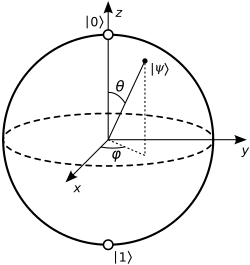
\includegraphics[width=0.3\textwidth]{Figures/Figura_3_1_1.png}
    \caption{Esfera de Bloch: representación geométrica de un qubit. 
    El estado $|\psi\rangle$ se representa como un punto en la 
    superficie de la esfera, determinado por los ángulos $\theta$ y 
    $\varphi$.}
    \label{fig:bloch}
\end{figure}

% ---
% Reemplaza líneas 1037-1092 de Docs/Technical_Report.tex
% Decisiones: N/A (sin cambio)
% ---

\subsubsection{Compuertas cuánticas de un qubit}
% -----------------------------------------------------------

Las operaciones sobre qubits se realizan mediante \textit{compuertas cuánticas}, representadas por matrices unitarias $U \in \mathbb{C}^{2\times 2}$ que satisfacen $UU^\dagger = I$. La unitariedad garantiza la reversibilidad de la operación y la conservación de la norma del estado. Las compuertas más relevantes para los circuitos variacionales son las rotaciones parametrizadas alrededor de los ejes de la esfera de Bloch \cite{nielsen2010quantum}:

\begin{equation}
    R_X(\theta) = e^{-i\frac{\theta}{2}X} = 
    \begin{pmatrix} 
        \cos\frac{\theta}{2}  & -i\sin\frac{\theta}{2} \\ 
        -i\sin\frac{\theta}{2} & \cos\frac{\theta}{2} 
    \end{pmatrix}
    \label{eq:rx}
\end{equation}

\begin{equation}
    R_Y(\theta) = e^{-i\frac{\theta}{2}Y} = 
    \begin{pmatrix} 
        \cos\frac{\theta}{2}  & -\sin\frac{\theta}{2} \\ 
        \sin\frac{\theta}{2}  & \cos\frac{\theta}{2} 
    \end{pmatrix}
    \label{eq:ry}
\end{equation}

\begin{equation}
    R_Z(\theta) = e^{-i\frac{\theta}{2}Z} = 
    \begin{pmatrix} 
        e^{-i\frac{\theta}{2}} & 0 \\ 
        0 & e^{i\frac{\theta}{2}} 
    \end{pmatrix}
    \label{eq:rz}
\end{equation}

\noindent donde $X$, $Y$ y $Z$ son las matrices de Pauli:

\begin{equation}
    X = \begin{pmatrix} 0 & 1 \\ 1 & 0 \end{pmatrix}, \quad
    Y = \begin{pmatrix} 0 & -i \\ i & 0 \end{pmatrix}, \quad
    Z = \begin{pmatrix} 1 & 0 \\ 0 & -1 \end{pmatrix}
    \label{eq:pauli}
\end{equation}

Estas compuertas de rotación son los bloques de construcción del ansatz variacional implementado en Qiskit, donde los ángulos $\theta$ son los parámetros entrenables del circuito. La compuerta de Hadamard, definida como:

\begin{equation}
    H = \frac{1}{\sqrt{2}}\begin{pmatrix} 1 & 1 \\ 1 & -1 
    \end{pmatrix}
    \label{eq:hadamard}
\end{equation}

\noindent transforma el estado base $|0\rangle$ en la 
superposición uniforme 
$\frac{1}{\sqrt{2}}(|0\rangle + |1\rangle)$, y es 
ampliamente utilizada como compuerta de inicialización en 
circuitos cuánticos.

% ---
% Reemplaza líneas 1093-1138 de Docs/Technical_Report.tex
% Decisiones: N/A (sin cambio)
% ---

\subsubsection{Sistemas de múltiples qubits y entrelazamiento}
% -----------------------------------------------------------

El estado de un sistema de $n$ qubits se describe mediante el producto tensorial de los espacios de Hilbert individuales:

\begin{equation}
    \mathcal{H}^{\otimes n} = 
    \underbrace{\mathbb{C}^2 \otimes \mathbb{C}^2 \otimes 
    \cdots \otimes \mathbb{C}^2}_{n}, 
    \quad \dim(\mathcal{H}^{\otimes n}) = 2^n
    \label{eq:tensor}
\end{equation}

\noindent El estado general de $n$ qubits es una superposición 
de los $2^n$ estados de la base computacional 
$\{|0\cdots0\rangle, |0\cdots1\rangle, \ldots, 
|1\cdots1\rangle\}$:

\begin{equation}
    |\Psi\rangle = \sum_{k=0}^{2^n - 1} c_k |k\rangle, 
    \quad c_k \in \mathbb{C}, 
    \quad \sum_{k=0}^{2^n-1} |c_k|^2 = 1
    \label{eq:multiQubit}
\end{equation}

El \textit{entrelazamiento cuántico} es la propiedad por la cual el estado de un sistema de múltiples qubits no puede factorizarse como el producto tensorial de estados individuales. Un estado entrelazado no tiene representación separable y exhibe correlaciones entre qubits que no tienen análogo clásico \cite{nielsen2010quantum}. La compuerta estándar para generar entrelazamiento es la \textit{compuerta CNOT} (Controlled-NOT), que opera sobre dos qubits: un qubit de control $c$ y un qubit objetivo $t$, aplicando una negación al objetivo condicionada al estado del control:

\begin{equation}
    \text{CNOT} = 
    \begin{pmatrix} 
        1 & 0 & 0 & 0 \\ 
        0 & 1 & 0 & 0 \\ 
        0 & 0 & 0 & 1 \\ 
        0 & 0 & 1 & 0 
    \end{pmatrix}
    \label{eq:cnot}
\end{equation}

\noindent La combinación de compuertas de rotación de un qubit 
y compuertas CNOT es suficiente para aproximar cualquier 
operación unitaria sobre $n$ qubits, propiedad conocida como 
\textit{universalidad} \cite{nielsen2010quantum}. Esta 
combinación es precisamente la que estructura el ansatz 
variacional RealAmplitudes utilizado en el presente trabajo.

% ---
% Reemplaza líneas 1139-1190 de Docs/Technical_Report.tex
% Decisiones: D-014, D-040, H-019, H-052
% ---

\subsubsection{Medición y valores de expectativa}

La medición en computación cuántica extrae información clásica del estado cuántico
al precio de colapsar la superposición. Para un observable $\hat{O}$ representado
por un operador hermítico, el valor de expectativa cuantifica el promedio estadístico
obtenido al medir dicho observable sobre un ensamble de estados idénticos $|\psi\rangle$:
\begin{equation}
  \langle \hat{O} \rangle = \langle \psi | \hat{O} | \psi \rangle.
  \label{eq:expectation}
\end{equation}
En el presente trabajo, los observables corresponden a las matrices
de Pauli $Z$ aplicadas a cada qubit individual $i \in \{1, \dots, n\}$. Su valor
de expectativa está en el intervalo $[-1, 1]$:
\begin{equation}
  \langle Z_i \rangle = \langle \psi | Z_i | \psi \rangle \in [-1, 1],
  \label{eq:expZ}
\end{equation}
donde $\langle Z_i \rangle = +1$ denota el estado computacional $|0\rangle$,
$\langle Z_i \rangle = -1$ denota el estado $|1\rangle$, y valores intermedios
describen superposiciones coherentes o mezclas estadísticas. El vector ordenado de
expectativas:
\begin{equation}
  \mathbf{e}_Z = \bigl(\langle Z_1 \rangle, \langle Z_2 \rangle, \dots, \langle Z_n \rangle\bigr)^\top \in [-1, 1]^n
  \label{eq:expZ_vector}
\end{equation}
resume la proyección del estado cuántico sobre cada qubit.

En un dispositivo físico cuántico, $\langle Z_i \rangle$ no se mide de forma
directa sino que se estima mediante el promedio de $n_{\text{shots}}$ mediciones
proyectivas independientes. Dado que los autovalores de $Z_i$ son $\pm 1$, cada disparo da $\pm 1$ con probabilidad $P(+1) = (1+\langle Z_i\rangle)/2$, de modo que la varianza de un disparo individual es $1-\langle Z_i\rangle^2$. La varianza del estimador empírico
$\hat{Z}_i = \frac{1}{n_{\text{shots}}} \sum_{s=1}^{n_{\text{shots}}} z_i^{(s)}$
está determinada exactamente por:
\begin{equation}
  \operatorname{Var}(\hat{Z}_i) = \frac{1 - \langle Z_i \rangle^2}{n_{\text{shots}}}.
  \label{eq:shot_noise_variance}
\end{equation}
La dispersión muestral es máxima cuando el estado es puramente ecuatorial
($\langle Z_i \rangle = 0$, varianza $1/n_{\text{shots}}$) y se anula si el qubit
se halla en un autoestado de la base computacional ($\langle Z_i \rangle = \pm 1$).

El núcleo de fidelidad cuántica, $K_Q(\mathbf{x}, \mathbf{x}') = |\langle \phi(\mathbf{x}) | \phi(\mathbf{x}') \rangle|^2$,
se estima en hardware de otra forma: se implementa el circuito de
\textit{compute-uncompute} $U^\dagger(\mathbf{x}') U(\mathbf{x})$ sobre el estado
$|0\rangle^{\otimes n}$ y se cuenta la frecuencia con la que se registra
la cadena nula $|0\dots 0\rangle$. Por lo tanto, la estimación del kernel en hardware
es un proceso binomial con probabilidad de éxito $p = K_Q$, cuya
varianza muestral es $K_Q(1 - K_Q)/n_{\text{shots}}$.

En la metodología principal del presente trabajo, con objeto de evaluar las
propiedades geométricas de las representaciones sin el ruido
que introduce un número finito de disparos, los valores de
expectativa y las matrices de fidelidad se evalúan analíticamente en simulación a
partir del vector de estado exacto (\textit{statevector}). El impacto empírico y
analítico de la cota finita de disparos ($n_{\text{shots}}$) se analiza de forma
explícita en el módulo de restricciones del simulador (M8).

% ---
% Reemplaza líneas 1191-1229 de Docs/Technical_Report.tex
% Decisiones: N/A (sin cambio)
% ---

\subsection{Circuitos cuánticos variacionales y 
            \textit{quantum embeddings}}

% -----------------------------------------------------------
\subsubsection{Circuitos cuánticos parametrizados (PQC)}
% -----------------------------------------------------------

Un \textit{circuito cuántico parametrizado} (PQC, por sus
siglas en inglés) es un circuito cuántico cuyas compuertas
dependen de un conjunto de parámetros reales
$\boldsymbol{\theta} \in \mathbb{R}^m$ que pueden ajustarse
mediante optimización clásica \cite{cerezo2021variational}.
Un \textit{circuito cuántico variacional} (VQC) es un tipo
específico de PQC que combina un bloque de codificación de
datos $U(\mathbf{x})$ con un bloque variacional entrenable
$W(\boldsymbol{\theta})$, produciendo el estado cuántico:

\begin{equation}
  |\psi(\mathbf{x}, \boldsymbol{\theta})\rangle =
  W(\boldsymbol{\theta})\,U(\mathbf{x})\,
  |0\rangle^{\otimes n}
  \label{eq:vqc_state}
\end{equation}

\noindent donde $n$ es el número de qubits,
$U(\mathbf{x})$ es el \textit{feature map} cuántico que
codifica el vector de características clásico
$\mathbf{x} \in \mathbb{R}^k$ en el estado cuántico inicial,
y $W(\boldsymbol{\theta})$ es el \textit{ansatz} variacional
que introduce correlaciones entre qubits mediante compuertas
entrenables \cite{Schuld2019QuantumML}.

La arquitectura VQC es la más adecuada para el régimen NISQ
actual porque mantiene profundidades de circuito moderadas
y es diferenciable de extremo a extremo mediante el método
de \textit{parameter-shift}, descrito en la
sección~\ref{sec:parameter_shift}.

% ---
% Reemplaza líneas 1230-1274 de Docs/Technical_Report.tex
% Decisiones: N/A (sin cambio)
% ---

\subsubsection{El \textit{feature map} como mapeo no lineal al espacio de Hilbert}
\label{sec:feature_map}
% -----------------------------------------------------------

El bloque $U(\mathbf{x})$ define un mapeo no lineal:

\begin{equation}
  \phi: \mathbb{R}^k \rightarrow \mathcal{H}, \qquad
  \mathbf{x} \mapsto |\phi(\mathbf{x})\rangle =
  U(\mathbf{x})\,|0\rangle^{\otimes n}
  \label{eq:feature_map}
\end{equation}

\noindent donde $\mathcal{H} = \mathbb{C}^{2^n}$ es el
espacio de Hilbert del sistema de $n$ qubits, de dimensión
$2^n$. Como se argumentó en la sección del planteamiento
del problema, este espacio no es simplemente una versión
ampliada del espacio clásico de entrada: su geometría está
determinada por productos internos cuánticos
$\langle\phi(\mathbf{x})|\phi(\mathbf{x}')\rangle$, no por
distancias euclidianas. Con compuertas de entrelazamiento,
el mapeo $\phi$ hace depender el estado de productos de pares
de componentes de $\mathbf{x}$ además de cada componente por
separado \cite{Schuld2019QuantumML, havlicek2019supervised}; si
la geometría resultante aporta separabilidad frente a un kernel
clásico es una pregunta empírica, que es la que aborda este trabajo.
% Corregido el 2026-10-19 (auditoría A5-1): decía «correlaciones de orden superior que los métodos
% clásicos no capturan», en contradicción con §2.1.3 y §3.2.4 (interacciones de dos cuerpos como máximo).

Este mapeo define implícitamente un \textit{kernel cuántico}:

\begin{equation}
  k_Q(\mathbf{x}, \mathbf{x}') =
  \left|\langle\phi(\mathbf{x})|\phi(\mathbf{x}')\rangle
  \right|^2 =
  \left|\langle 0|^{\otimes n}\,U^\dagger(\mathbf{x}')\,
  U(\mathbf{x})\,|0\rangle^{\otimes n}\right|^2
  \label{eq:quantum_kernel}
\end{equation}

\noindent La elección del \textit{feature map} $U(\mathbf{x})$
determina completamente la geometría del espacio de
representación y, con ello, la capacidad del sistema para
separar las clases en ese espacio. En el presente trabajo
se comparan dos diseños de \textit{feature map}:
\textit{ZZFeatureMap} y \textit{PauliFeatureMap},
descritos a continuación.

% ---
% Reemplaza líneas 1275-1346 de Docs/Technical_Report.tex
% Decisiones: D-031, H-031
% ---

\subsubsection{\textit{ZZFeatureMap}: evolución de Pauli-Z de segundo orden}

El \textit{ZZFeatureMap} es un circuito de evolución de
Pauli-Z de segundo orden introducido por Havlíček et al.
\cite{havlicek2019supervised} y disponible en Qiskit como
\texttt{zz\_feature\_map}.
Para $n$ qubits y $r$ repeticiones (\texttt{reps}),
el circuito implementa el unitario:

\begin{equation}
  U_{\text{ZZ}}(\mathbf{x}) =
  \left[\mathcal{U}_\Phi(\mathbf{x})\,H^{\otimes n}
  \right]^r
  \label{eq:zzfeaturemap}
\end{equation}

\noindent donde $H^{\otimes n}$ es la capa de compuertas
de Hadamard que inicializa la superposición uniforme, y
$\mathcal{U}_\Phi(\mathbf{x})$ es el bloque de codificación
de datos definido por\footnote{Havlíček et al. y la documentación de Qiskit escriben $+i$; el circuito de Qiskit implementa $-i$, que produce el estado complejo conjugado. El kernel de fidelidad y los valores esperados de este trabajo no dependen de esa elección.}:

\begin{equation}
  \mathcal{U}_\Phi(\mathbf{x}) =
  \exp\!\left(-i \sum_{S \subseteq [n],\,|S|\leq 2}
  \phi_S(\mathbf{x})\,\bigotimes_{j \in S} Z_j\right)
  \label{eq:Uphi}
\end{equation}

\noindent Los coeficientes $\phi_S(\mathbf{x})$ codifican
los datos clásicos en el hamiltoniano de evolución:

\begin{equation}
  \phi_{\{i\}}(\mathbf{x}) = x_i, \qquad
  \phi_{\{i,j\}}(\mathbf{x}) =
  (\pi - x_i)(\pi - x_j)
  \label{eq:phi_coefficients}
\end{equation}

Como $e^{-i\phi Z} = \operatorname{diag}(e^{-i\phi}, e^{i\phi})$, cada término introduce una fase
relativa $2\phi_S$ entre las componentes del estado. Por eso el circuito de Qiskit aplica
compuertas de fase $P(2x_i)$ y $P\bigl(2(\pi-x_i)(\pi-x_j)\bigr)$: el factor 2 corresponde al
parámetro \texttt{alpha} de la función, cuyo valor por defecto es 2. Con $x_i\in[0,\pi]$, la fase
relativa propia recorre la circunferencia una vez.

\noindent El término de un qubit $\phi_{\{i\}}$ codifica
cada característica $x_i$ como una rotación alrededor del
eje $Z$. El término de dos qubits $\phi_{\{i,j\}}$
introduce \textit{entrelazamiento} entre pares de qubits
que codifica las interacciones de segundo orden entre
características, operando mediante la compuerta:

\begin{equation}
  e^{i\,\phi_{\{i,j\}}(\mathbf{x})\,Z_i Z_j} =
  \text{CNOT}_{i \to j}\;
  e^{i\,\phi_{\{i,j\}}(\mathbf{x})\,Z_j}\;
  \text{CNOT}_{i \to j}
  \label{eq:zz_gate}
\end{equation}

\noindent Esta capacidad de capturar interacciones de segundo
orden entre pares de características es la razón por la que
el ZZFeatureMap es uno de los métodos
de codificación de datos más utilizados en tareas de
clasificación cuántica, dada su capacidad para enriquecer la
expresividad del espacio de características cuántico y la
dificultad de simularlo clásicamente. 

Es importante señalar que en Qiskit 2.x el uso de la clase
\texttt{ZZFeatureMap} está marcado como obsoleto
(\textit{deprecated}) a favor de la función
\texttt{zz\_feature\_map()}, que retorna un
\texttt{QuantumCircuit} estándar \cite{ibmquantum2024docs}.
En el presente trabajo se utiliza la función actualizada
compatible con Qiskit 2.x.

% ---
% Reemplaza líneas 1347-1390 de Docs/Technical_Report.tex
% Decisiones: D-031, H-012, H-034
% ---

\subsubsection{\textit{PauliFeatureMap}: generalización por elección de los operadores de Pauli}

El circuito \textit{PauliFeatureMap} constituye la generalización del esquema de
Havl{\'{\i}}{\v{c}}ek et al. que permite seleccionar subconjuntos arbitrarios de
operadores de Pauli ($X$, $Y$, $Z$) en el bloque unitario de codificación. El operador
adopta la forma general:
\begin{equation}
  U_{\text{Pauli}}(\mathbf{x}) = \left[\mathcal{U}_\Phi^{(P)}(\mathbf{x})\,H^{\otimes n}\right]^r,
  \label{eq:paulifeaturemap}
\end{equation}
donde el generador diagonal o no diagonal se define a partir de una familia de cadenas
de Pauli $\{P_S\}$:
\begin{equation}
  \mathcal{U}_\Phi^{(P)}(\mathbf{x}) = \prod_{P \in \mathcal{P}}
  \exp\!\left(-i \sum_{S} \phi_S(\mathbf{x})\,\bigotimes_{j \in S} P_j\right),
  \label{eq:pauli_expansion}
\end{equation}
donde $\mathcal{P}$ es la lista de cadenas de Pauli elegida, en el orden en que se aplican. Si los
términos no conmutan, como $Y$ y $ZZ$, el bloque es un producto de exponenciales y no una
sola exponencial: en C5 se aplica primero $\exp\bigl(-i\sum_i x_i Y_i\bigr)$ y después
$\exp\bigl(-i\sum_{i<j}(\pi-x_i)(\pi-x_j)Z_iZ_j\bigr)$.
En el presente trabajo, la condición experimental C5 se define formalmente como
\texttt{pauli\_feature\_map(paulis=['Y', 'ZZ'], reps=1)}, manteniendo el mismo número
de qubits ($k = 12$) e idéntica conectividad de entrelazamiento de segundo orden
($ZZ$) que el mapa C4 (\texttt{zz\_feature\_map}). La
comparación entre C4 y C5 aísla con precisión el efecto de sustituir el eje de rotación
de la codificación de primer orden (eje $Z$ frente a eje $Y$), preservando
inalterada la estructura del entrelazamiento de dos cuerpos.

La elección de operadores de Pauli en la codificación de un solo qubit tiene consecuencias
geométricas sobre la esfera de Bloch:
\begin{enumerate}
  \item \textbf{El término en $X$ no codifica nada:} Tras la capa inicial de Hadamard,
        el estado del registro se encuentra en $|+\rangle^{\otimes n} = \left(\frac{|0\rangle + |1\rangle}{\sqrt{2}}\right)^{\otimes n}$.
        Dado que el estado $|+\rangle$ es un autoestado del operador de Pauli $X$ con
        autovalor $+1$ ($X|+\rangle = |+\rangle$), la aplicación del operador unitario de
        evolución bajo $X$ satisface:
        \begin{equation}
          e^{-i\,\phi(x_i)\,X}|+\rangle = e^{-i\,\phi(x_i)}\,|+\rangle.
          \label{eq:x_eigenstate_phase}
        \end{equation}
        La variable $x_i$ induce únicamente una fase global no física sobre el qubit, sin
        alterar las amplitudes relativas ni modificar la densidad de probabilidad en
        ninguna base. Un mapa basado en $\{X, ZZ\}$ anula la codificación
        de primer orden y degenera en un circuito de puro entrelazamiento $ZZ$.
  \item \textbf{Rotación a lo largo del ecuador (Pauli $Z$, C4):} El generador $Z$ desplaza
        el estado $|+\rangle$ a lo largo del plano ecuatorial de la esfera de Bloch, alterando
        la fase relativa $\varphi$ entre $|0\rangle$ y $|1\rangle$ sin cambiar las
        probabilidades marginales de ocupación de los polos.
  \item \textbf{Rotación fuera del ecuador hacia los polos (Pauli $Y$, C5):} El generador
        $Y$ actúa perpendicularmente al estado ecuatorial $|+\rangle$, rotándolo a lo largo
        de un meridiano hacia los polos $|0\rangle$ y $|1\rangle$. Esta transformación
        modifica de forma directa las probabilidades de medición en la base computacional
        antes de la aplicación del entrelazamiento.
\end{enumerate}

Qiskit construye el término $\exp(-i x_i Y)$ como $\sqrt{X}\,P(2x_i)\,\sqrt{X}^\dagger$, que equivale a $R_Y(2x_i)$ salvo una fase global. La condición C5 añade 12 compuertas
$\sqrt{X}$ (\texttt{SX}) y 12 compuertas $\sqrt{X}^\dagger$ (\texttt{SXdg}) respecto a C4,
con lo que la profundidad del circuito pasa de 65 a 67 capas, sin compuertas CNOT
adicionales. Al restringirse ambos mapas a interacciones de grado $|S| \le 2$, C5
no introduce interacciones de orden superior respecto a C4.

% ---
% Reemplaza líneas 1391-1421 de Docs/Technical_Report.tex
% Decisiones: D-014, H-011, H-054
% ---

\subsubsection{El \textit{ansatz} variacional: RealAmplitudes}

El bloque variacional $W(\boldsymbol{\theta})$ introduce capas de rotaciones
parametrizadas y compuertas de entrelazamiento destinadas a manipular las amplitudes
del estado codificado $|\phi(\mathbf{x})\rangle$. En este trabajo se emplea la
función \texttt{real\_amplitudes} de Qiskit 2.x, compuesta por una capa inicial de
rotaciones $R_Y$ seguida de $r$ bloques repetidos con una cadena de CNOT entre qubits vecinos y nuevas rotaciones $R_Y$:
\begin{equation}
  W(\boldsymbol{\theta}) = \left[\prod_{\ell=r}^{1} \Bigl(\bigotimes_{i=1}^{n} R_Y(\theta_{\ell,i})\Bigr)\, E \right] \bigotimes_{i=1}^{n} R_Y(\theta_{0,i}),
  \label{eq:real_amplitudes}
\end{equation}
donde $E$ es la cadena de CNOT, $r$ es el número de repeticiones (\texttt{reps}) y el producto se
escribe con $\ell$ creciente hacia la izquierda, que es el orden en que actúan las capas. Para
$r = 1$, $W(\boldsymbol{\theta}) = \bigl(\bigotimes_i R_Y(\theta_{1,i})\bigr)\,E\,\bigl(\bigotimes_i R_Y(\theta_{0,i})\bigr)$.
El número total de parámetros es:
\begin{equation}
  m = n\,(r + 1).
  \label{eq:num_params_ansatz}
\end{equation}
Para la configuración experimental fijada en este trabajo ($n = 12$ qubits y $r = 1$
repetición), el \textit{ansatz} contiene exactamente $m = 12 \times (1 + 1) = 24$
parámetros angulares $\boldsymbol{\theta} \in \mathbb{R}^{24}$. $R_Y$ y CNOT son matrices reales: aplicadas sobre $|0\rangle^{\otimes n}$ producirían solo amplitudes reales, de ahí el nombre. En este trabajo actúan sobre el estado complejo que deja el \textit{feature map}.

El \textit{ansatz} no puede suprimirse. En C4 (\texttt{zz\_feature\_map}), la codificación
aplica Hadamard seguido de compuertas diagonales ($Z$ y $ZZ$). Las compuertas
diagonales modifican las fases relativas pero preservan inalteradas las magnitudes de las
amplitudes complejas $|c_j| = 2^{-n/2}$. En consecuencia, medir el valor de expectativa
en la base $Z$ directamente tras el mapa de características produciría
$\langle Z_i \rangle = 0$ para cualquier entrada $\mathbf{x}$. La información reside
en las fases relativas del estado cuántico, a las que la medición en la base
computacional es ciega. En C5 el giro en $Y$ sí cambia las probabilidades, pero sin el \textit{ansatz} se tendría
$\langle Z_i\rangle = -\sin(2x_i)$: cada valor dependería de una sola característica y las fases
del acoplamiento $ZZ$ seguirían sin verse. El \textit{ansatz} $W(\boldsymbol{\theta})$ mezcla los
qubits y convierte parte de las diferencias de fase en diferencias de probabilidad medibles en
$\langle Z_i \rangle$.

% ---
% Reemplaza líneas 1422-1464 de Docs/Technical_Report.tex
% Decisiones: D-014, H-019, H-053
% ---

\subsubsection{El \textit{quantum embedding}: vector de salida del circuito}
\label{sec:quantum_embedding}

A partir del estado conjunto $|\psi(\mathbf{x}, \boldsymbol{\theta})\rangle = W(\boldsymbol{\theta})\,U(\mathbf{x})\,|0\rangle^{\otimes n}$,
el circuito extrae información mediante la medición del valor de expectativa del operador de Pauli $Z$ sobre cada qubit $i$:
\begin{equation}
  \langle Z_i \rangle = \langle \psi(\mathbf{x}, \boldsymbol{\theta}) | Z_i | \psi(\mathbf{x}, \boldsymbol{\theta}) \rangle \in [-1, 1].
  \label{eq:expval}
\end{equation}
El \textit{quantum embedding} de la muestra $\mathbf{x}$ se formaliza como el vector
de los $n$ valores de expectativa:
\begin{equation}
  \mathbf{e}(\mathbf{x}, \boldsymbol{\theta}) = \bigl(\langle Z_1 \rangle, \langle Z_2 \rangle, \dots, \langle Z_n \rangle\bigr)^\top \in [-1, 1]^n.
  \label{eq:embedding_vector}
\end{equation}
En el diseño adoptado, el vector de parámetros
$\boldsymbol{\theta}$ no se entrena mediante optimización iterativa supervisada: se fija
de forma determinista una sola vez mediante un sorteo uniforme en $[0, 2\pi)$ con
semilla declarada (42). Los valores de expectativa $\mathbf{e}(\mathbf{x}, \boldsymbol{\theta})$
se calculan analíticamente de forma exacta sobre el vector de estado (\textit{statevector})
y se almacenan para alimentar directamente a los clasificadores clásicos.

Por otra parte, la matriz de kernel de fidelidad cuántica $K_Q(\mathbf{x}, \mathbf{x}')$, definida en la ecuación~\eqref{eq:quantum_kernel}, se evalúa exclusivamente sobre el \textit{feature map} $U(\mathbf{x})$, sin incluir el \textit{ansatz} $W(\boldsymbol{\theta})$. Dado que $W(\boldsymbol{\theta})$ es un operador unitario ($W^\dagger W = I$), su inserción antes de la medición se cancelaría en el producto interno: $|\langle \phi(\mathbf{x}) | W^\dagger W | \phi(\mathbf{x}') \rangle|^2 = |\langle \phi(\mathbf{x}) | \phi(\mathbf{x}') \rangle|^2$.

% ---
% Reemplaza líneas 1465-1512 de Docs/Technical_Report.tex
% Decisiones: D-014, H-011, H-054
% ---

\subsubsection{El método \textit{parameter-shift} para el cálculo del gradiente}
\label{sec:parameter_shift}

Para la optimización de circuitos cuánticos variacionales en plataformas físicas, el
cálculo del gradiente de un valor de expectativa respecto a los parámetros del circuito
$\boldsymbol{\theta}$ no puede llevarse a cabo mediante la retropropagación clásica de
errores (\textit{backpropagation}), dado que el estado interno colapsa durante la medición
y las amplitudes intermedias son físicamente inaccesibles. En su lugar, se recurre a la
regla analítica del \textit{parameter-shift} \cite{mitarai2018quantum, cerezo2021variational}.
Para compuertas unitarias generadas por operadores hermíticos con dos autovalores
distintos (tales como las rotaciones de Pauli $R_Y(\theta) = \exp(-i \frac{\theta}{2} Y)$),
la derivada exacta del valor esperado viene dada por:
\begin{equation}
  \frac{\partial \langle Z_i \rangle}{\partial \theta_j} =
  \frac{1}{2}\left[
    \langle Z_i \rangle_{\theta_j + \frac{\pi}{2}} -
    \langle Z_i \rangle_{\theta_j - \frac{\pi}{2}}
  \right],
  \label{eq:parameter_shift}
\end{equation}
donde $\langle Z_i \rangle_{\theta_j \pm \pi/2}$ denota el valor de expectativa del circuito
evaluado sustituyendo el parámetro escalar $\theta_j$ por $\theta_j \pm \pi/2$, manteniendo
los demás parámetros constantes.

Con $m = n(r+1) = 24$ parámetros, cada gradiente por muestra exige $2m = 48$ evaluaciones del circuito. Medido en el simulador con valores exactos, el gradiente por \textit{parameter-shift} tardó 5.16~s por lesión, lo que para las 2\,864 lesiones de entrenamiento y 50 épocas representa unas 205~h por \textit{feature map}. La retropropagación a través del vector de estado produce el mismo gradiente (con una diferencia de $1.8\times10^{-15}$) en 3.4~min, unas 3\,600 veces menos tiempo, pero exige conocer simultáneamente las $2^n$ amplitudes del estado, información que un computador cuántico no entrega porque medir colapsa el estado. En este trabajo $\boldsymbol{\theta}$ no se entrena (sección~\ref{sec:modulo5}); el costo se documenta como parte del OE-6.

% ---
% Reemplaza líneas 1513-1584 de Docs/Technical_Report.tex
% Decisiones: N/A (sin cambio)
% ---

\subsection{Red neuronal clásica e integración
            Qiskit--PyTorch}

% -----------------------------------------------------------
\subsubsection{Perceptrón multicapa (MLP)}
% -----------------------------------------------------------

La red neuronal clásica utilizada como clasificador
\textit{downstream} en el pipeline del presente trabajo es
un perceptrón multicapa (MLP, \textit{Multi-Layer
Perceptron}), una arquitectura de aprendizaje supervisado
compuesta por capas de neuronas totalmente conectadas
\cite{goodfellow2016deep}.

Formalmente, dado un vector de entrada
$\mathbf{z} \in \mathbb{R}^n$, que puede ser el
\textit{quantum embedding}
$\mathbf{e}(\mathbf{x}, \boldsymbol{\theta})$ o cualquiera
de los vectores de las condiciones clásicas, la
transformación de la capa $\ell$ se define como:

\begin{equation}
  \mathbf{h}^{(\ell)} = \sigma\!\left(
  W^{(\ell)}\,\mathbf{h}^{(\ell-1)} + \mathbf{b}^{(\ell)}
  \right), \qquad \ell = 1, \ldots, L
  \label{eq:mlp_layer}
\end{equation}

\noindent donde $W^{(\ell)} \in \mathbb{R}^{d_\ell \times
d_{\ell-1}}$ es la matriz de pesos, $\mathbf{b}^{(\ell)}
\in \mathbb{R}^{d_\ell}$ es el vector de sesgos, y
$\sigma(\cdot)$ es la función de activación no lineal.
La capa de salida produce una probabilidad de clasificación
binaria mediante la función sigmoide:

\begin{equation}
  \hat{y} = \sigma_{\text{sig}}\!\left(
  W^{(L)}\,\mathbf{h}^{(L-1)} + b^{(L)}
  \right) =
  \frac{1}{1 + e^{-(W^{(L)}\mathbf{h}^{(L-1)}
  + b^{(L)})}}
  \in [0, 1]
  \label{eq:sigmoid_output}
\end{equation}

\noindent El modelo se entrena minimizando la función de
pérdida de entropía cruzada binaria (\textit{Binary
Cross-Entropy}, BCE):

\begin{equation}
  \mathcal{L}_{\text{BCE}}(\hat{y}, y) =
  -\left[y\log\hat{y} + (1-y)\log(1-\hat{y})\right]
  \label{eq:bce_loss}
\end{equation}

\noindent donde $y \in \{0, 1\}$ es la etiqueta real
(0\,=\,benigno, 1\,=\,maligno). Los parámetros
$\{W^{(\ell)}, \mathbf{b}^{(\ell)}\}$ se optimizan
mediante descenso de gradiente estocástico (\textit{Adam}
o equivalente) a través del algoritmo de
\textit{backpropagation} \cite{goodfellow2016deep}.

La arquitectura del MLP se mantiene idéntica para las cinco
condiciones experimentales: mismo número de capas ocultas,
mismas dimensiones, misma función de activación, mismos
hiperparámetros y misma semilla aleatoria. Esta
invarianza es el principio metodológico central que garantiza
que las diferencias de rendimiento entre condiciones sean
atribuibles únicamente a la transformación aplicada en M5,
y no a diferencias en el clasificador.

% ---
% Reemplaza líneas 1585-1617 de Docs/Technical_Report.tex
% Decisiones: N/A (sin cambio)
% ---

\subsubsection{Ponderación de clases para datos desbalanceados}
% -----------------------------------------------------------

Dado el desbalance de clases observado en el análisis
exploratorio del dataset CBIS-DDSM (ratio 1.78:1 en
calcificaciones), se aplica ponderación de clases durante
el entrenamiento del MLP. La pérdida ponderada se define
como:

\begin{equation}
  \mathcal{L}_w = -\left[
  w_1\,y\log\hat{y} +
  w_0\,(1-y)\log(1-\hat{y})
  \right]
  \label{eq:weighted_bce}
\end{equation}

\noindent donde los pesos $w_0$ y $w_1$ se calculan
inversamente proporcionales a la frecuencia de cada clase
en el conjunto de entrenamiento:

\begin{equation}
  w_c = \frac{N}{C \cdot N_c}, \qquad c \in \{0, 1\}
  \label{eq:class_weights}
\end{equation}

\noindent siendo $N$ el número total de muestras, $C = 2$
el número de clases y $N_c$ el número de muestras de la
clase $c$. Este ajuste se aplica de forma independiente
para los subconjuntos de masas y calcificaciones.

% ---
% Reemplaza líneas 1618-1668 de Docs/Technical_Report.tex
% Decisiones: D-014, H-011, H-054
% ---

\subsubsection{Integración cuántico-clásica: \textit{embeddings} precomputados}

La integración entre los circuitos cuánticos y el clasificador clásico se formula
mediante una arquitectura desacoplada basada en representaciones intermedias.
En lugar de ensamblar el circuito cuántico como una
capa diferenciable dentro de la red neuronal mediante adaptadores de software como
\texttt{TorchConnector} \cite{qiskitml2024}, el pipeline separa la fase
de transformación cuántica de la fase de clasificación supervisada.

El flujo de procesamiento opera de acuerdo con las siguientes etapas metodológicas:
\begin{enumerate}
  \item \textbf{Generación determinista de representaciones:} A partir del vector de
        características seleccionado y escalado $\mathbf{x} \in [0, \pi]^{12}$ (M4),
        el circuito cuántico compuesto por el mapa de características (\texttt{zz\_feature\_map}
        en C4 o \texttt{pauli\_feature\_map} en C5) y el \textit{ansatz} \texttt{real\_amplitudes}
        con parámetros fijos $\boldsymbol{\theta}$ calcula de forma analítica el vector
        de expectativas exactas $\mathbf{e}(\mathbf{x}, \boldsymbol{\theta}) \in [-1, 1]^{12}$.
  \item \textbf{Almacenamiento de representaciones:} Los vectores resultantes se
        precomputan una sola vez para la totalidad del conjunto de datos y se persisten
        en disco en formato estructurado, eliminando la necesidad de reevaluar circuitos
        durante el ciclo de optimización del clasificador.
  \item \textbf{Estandarización:} Los vectores de cada condición experimental
        se estandarizan empleando la media y desviación estándar ajustadas sobre el conjunto de entrenamiento de cada partición, compensando la disparidad
        en las escalas numéricas de las distintas condiciones (M7).
  \item \textbf{Entrenamiento del clasificador clásico:} El perceptrón multicapa (MLP)
        en PyTorch se entrena sobre las representaciones estandarizadas,
        optimizando sus pesos sin modificar los parámetros del circuito cuántico.
\end{enumerate}

Este diseño responde a tres razones:
\begin{itemize}
  \item \textbf{Validez interna del experimento:} Las condiciones clásicas C2 (PCA) y
        C3 (Kernel PCA) operan como transformaciones no supervisadas que no acceden a las
        etiquetas de patología para construir el nuevo espacio. Si C4 y C5 ajustaran
        $\boldsymbol{\theta}$ contra las etiquetas durante el entrenamiento, cualquier
        ganancia en clasificación podría atribuirse al ajuste paramétrico supervisado y no
        a las propiedades geométricas de la codificación cuántica $\phi$.
  \item \textbf{Correspondencia con la pregunta de investigación:} El objetivo del trabajo
        consiste en determinar en qué medida el mapeo cuántico al espacio de Hilbert modifica
        la separabilidad intrínseca de las características radiómicas, aislando la capacidad
        representacional del \textit{feature map} frente a la optimización variacional.
  \item \textbf{Viabilidad computacional:} Evita el costo de cientos de horas de ejecución
        que demandaría el método \textit{parameter-shift} en cada época de entrenamiento; en el simulador la retropropagación sobre el vector de estado abarataría el entrenamiento, pero ese atajo no existe en hardware (sección~\ref{sec:parameter_shift}).
\end{itemize}

% ---
% Reemplaza líneas 1669-1709 de Docs/Technical_Report.tex
% Decisiones: D-014, H-011, H-052
% ---

\subsubsection{Implementación en Qiskit 2.x}

En Qiskit 2.x, el flujo computacional del pipeline se estructura en los siguientes pasos:
\begin{enumerate}
  \item Construcción del \textit{feature map} con \texttt{zz\_feature\_map(12, reps=1)} o \texttt{pauli\_feature\_map(12, reps=1, paulis=['Y','ZZ'])}.
  \item Instanciación del \textit{ansatz} con \texttt{real\_amplitudes(12, reps=1)} y vector de parámetros $\boldsymbol{\theta}$ sorteado una sola vez con semilla determinista 42.
  \item Composición del circuito y asignación fija de parámetros mediante los métodos \texttt{compose} y \texttt{assign\_parameters}.
  \item Cálculo del vector de estado mediante la clase \texttt{Statevector} y obtención de los valores de expectativa $\langle Z_i\rangle = \sum_b p(b)\,(1-2b_i)$ a partir de las probabilidades exactas de la base computacional.
  \item Evaluación del núcleo de fidelidad cuántica mediante la clase \texttt{FidelityStatevectorKernel} de \texttt{qiskit-machine-learning}.
\end{enumerate}

En este trabajo no se usan \texttt{EstimatorQNN} ni \texttt{TorchConnector}. \texttt{EstimatorQNN} solicita por defecto una precisión de $0.015625$, y con ella la primitiva \texttt{StatevectorEstimator} suma a cada valor esperado un ruido gaussiano de esa desviación; el \texttt{EstimatorV2} de Qiskit Aer tampoco muestrea, sino que devuelve el valor exacto más un ruido gaussiano de la precisión pedida. Por eso, en este trabajo, «exacto» significa vector de estado directo o precisión cero explícita, y el estudio de \textit{shots} se hace con un muestreo de las probabilidades exactas.

Es importante señalar que las clases \texttt{ZZFeatureMap}, \texttt{PauliFeatureMap} y \texttt{RealAmplitudes} están marcadas como obsoletas en Qiskit 2.x a favor de las funciones \texttt{zz\_feature\_map()}, \texttt{pauli\_feature\_map()} y \texttt{real\_amplitudes()}, que retornan un \texttt{QuantumCircuit} estándar en lugar de un \texttt{BlueprintCircuit} \cite{ibmquantum2024docs}. El presente trabajo utiliza las funciones actualizadas para garantizar compatibilidad con Qiskit 2.x.

% ---
% Reemplaza líneas 1710-1720 de Docs/Technical_Report.tex
% Decisiones: N/A (estructura base)
% ---

\subsection{Métricas de separabilidad y evaluación}
\label{sec:metricas}

Este bloque formaliza las métricas utilizadas para evaluar
las representaciones generadas por cada condición
experimental. Se organizan en dos grupos: métricas de
separabilidad, que miden la calidad del espacio de
representación con independencia del clasificador; y
métricas de clasificación, que miden el desempeño del
MLP sobre cada representación.

% ---
% Reemplaza líneas 1721-1760 de Docs/Technical_Report.tex
% Decisiones: D-033, H-038
% ---

\subsubsection{\textit{Kernel-Target Alignment} (KTA)}

El \textit{Kernel-Target Alignment} (KTA) cuantifica la similitud entre una matriz de
kernel $K \in \mathbb{R}^{N \times N}$ evaluada sobre $N$ muestras y la matriz de etiquetas
ideales de clasificación $Y = \mathbf{y}\mathbf{y}^\top$, donde $\mathbf{y} \in \{-1, +1\}^N$
denota el vector de etiquetas binarias de patología.

La formulación original propuesta por Cristianini et al. \cite{cristianini2002kernel}
define la alineación no centrada como el coseno de Frobenius entre ambas matrices:
\begin{equation}
  \widehat{\text{KTA}}_u(K, \mathbf{y}) =
  \frac{\langle K, \mathbf{y}\mathbf{y}^\top \rangle_F}{\|K\|_F \cdot \|\mathbf{y}\mathbf{y}^\top\|_F} =
  \frac{\mathbf{y}^\top K \mathbf{y}}{N\,\|K\|_F},
  \label{eq:kta_uncentered}
\end{equation}
donde $\langle A, B \rangle_F = \operatorname{Tr}(A^\top B) = \sum_{i,j} A_{ij} B_{ij}$ es el
producto interno de Frobenius y $\|\cdot\|_F$ su norma inducida. Dado que $y_i \in \{-1, +1\}$,
la norma de la matriz de etiquetas ideales satisface $\|\mathbf{y}\mathbf{y}^\top\|_F = N$.

No obstante, la métrica no centrada presenta un sesgo ante conjuntos de datos con
desbalance de clases. Si la proporción de clases difiere del 50\,\%, el valor esperado de
$y_i y_j$ es positivo, lo que provoca que una matriz de kernel no informativa
(e.g., una matriz constante u homogénea) obtenga valores elevados
de alineación simplemente por capturar la media de las etiquetas. Para suprimir este artefacto,
Cortes, Mohri y Rostamizadeh \cite{Cortes2012} introdujeron la \textit{alineación de kernel centrada}
(\textit{Centered Kernel Alignment}), adoptada en este trabajo como la métrica principal de KTA:
\begin{equation}
  \widehat{\text{KTA}}_c(K, \mathbf{y}) =
  \frac{\langle K_c, (\mathbf{y}\mathbf{y}^\top)_c \rangle_F}{\|K_c\|_F \cdot \|(\mathbf{y}\mathbf{y}^\top)_c\|_F} =
  \frac{\mathbf{y}^\top K_c \mathbf{y}}{\|K_c\|_F\,\sum_{i=1}^N (y_i - \bar{y})^2},
  \label{eq:kta_centered}
\end{equation}
donde $K_c = H K H$ representa la matriz de kernel centrada mediante la matriz de proyección
$H = I - \frac{1}{N}\mathbf{1}\mathbf{1}^\top$, con componentes escalares:
\begin{equation}
  (K_c)_{ij} = K_{ij} - \frac{1}{N}\sum_{k=1}^N K_{ik} - \frac{1}{N}\sum_{l=1}^N K_{lj} + \frac{1}{N^2}\sum_{k,l=1}^N K_{kl}.
  \label{eq:kernel_centering_scalar}
\end{equation}
El término de normalización $\|(\mathbf{y}\mathbf{y}^\top)_c\|_F$ coincide con la
suma de desviaciones cuadráticas de las etiquetas centradas, $\sum_{i=1}^N (y_i - \bar{y})^2$.

A pesar del centrado, los kernels que presentan concentración exhiben una cota
inferior analítica fija. Para la matriz identidad $K = I$ (el kernel de un espacio donde todas
las muestras son mutuamente ortogonales), la KTA centrada adopta un valor
constante e independiente de las etiquetas:
\begin{equation}
  \widehat{\text{KTA}}_c(I, \mathbf{y}) = \frac{1}{\sqrt{N - 1}},
  \label{eq:kta_identity_floor}
\end{equation}
que para la submuestra de evaluación de $N = 200$ lesiones equivale a $1/\sqrt{199} \approx 0.0709$.
(Para la formulación no centrada, dicho valor equivale a $1/\sqrt{N} = 1/\sqrt{200} \approx 0.0707$).
En consecuencia, las magnitudes absolutas de KTA no son directamente comparables entre kernels
cuyos espectros de autovalores difieren mucho. Para establecer una comparación válida,
la alineación de cada kernel se evalúa calculando el \textit{exceso de alineación} respecto a
la media de una prueba de permutación con $1\,000$ barajadas de las etiquetas que
conservan el número de lesiones de cada clase:
\begin{equation}
  \Delta\text{KTA}_c = \widehat{\text{KTA}}_c(K, \mathbf{y}) - \mathbb{E}_{\pi}\left[\widehat{\text{KTA}}_c(K, \mathbf{y}_\pi)\right].
  \label{eq:kta_excess}
\end{equation}
Para C4 y C5 el kernel es el de fidelidad (ecuación~\eqref{eq:quantum_kernel}); la referencia clásica es el RBF con $\gamma$ fijado por la heurística de la mediana; sobre los vectores de cada condición se calcula además la KTA del kernel lineal.

% ---
% Reemplaza líneas 1761-1802 de Docs/Technical_Report.tex
% Decisiones: D-028, D-032, H-033, H-038
% ---

\subsubsection{\textit{Geometric difference}}

La \textit{geometric difference} fue formalizada por Huang et al. \cite{huang2021power}
para evaluar si un kernel cuántico $K_Q$ induce sobre los datos una geometría que un kernel
clásico $K_C$ dado no puede reproducir.
Dados $K_Q, K_C \in \mathbb{R}^{N \times N}$ normalizados a traza común $\operatorname{Tr}(K_Q) = \operatorname{Tr}(K_C) = N$,
la \textit{geometric difference} sin regularizar es:
\begin{equation}
  g_{CQ} = g(K_C \parallel K_Q) = \sqrt{\left\| \sqrt{K_Q}\;K_C^{-1}\;\sqrt{K_Q} \right\|_\infty},
  \label{eq:geometric_diff}
\end{equation}
donde $\|\cdot\|_\infty$ denota la norma espectral (el autovalor máximo de la matriz simétrica)
y $\sqrt{K}$ es la raíz cuadrada matricial simétrica positiva obtenida por descomposición
espectral:
\begin{equation}
  K = V \Lambda V^\top \implies \sqrt{K} = V \Lambda^{1/2} V^\top,
  \label{eq:spectral_sqrt}
\end{equation}
con truncamiento a cero de posibles autovalores residuales negativos por precisión de punto
flotante. En la ecuación~\eqref{eq:geometric_diff}, el kernel cuántico $K_Q$ figura en los
factores externos mientras que el kernel clásico $K_C$ es la matriz invertida.
Con kernels de diagonal unitaria y $\operatorname{Tr}K=N$, $g_{CQ}\ge1$: basta evaluar el cociente de Rayleigh $v^\top K_Q v / v^\top K_C v$ en un vector canónico.

En conjuntos de datos reales, la evaluación directa de la ecuación~\eqref{eq:geometric_diff}
resulta numéricamente inestable debido a que las matrices de kernel clásicas suelen presentar
valores propios muy pequeños, que disparan $g_{CQ}$ y hacen que mida el condicionamiento de $K_C$ y no la codificación. Para subsanar esto, Huang et al. \cite{huang2021power} definieron
% respaldo: «When we only have a finite number N of training samples, we can use the fact that k(x, y) = φ(x)†φ(y) and the definition that Kij = k(xi, xj) to obtain» (huang2021powerSupp, p. 12)
% Equivalencias con la versión de arXiv (2011.01938): sección 6 C = Apéndice F.3; (S71) = (F19); (S72) = (F20).
la formulación regularizada mediante un parámetro de penalización $\lambda > 0$ (información suplementaria, sección~6\,C, ecs.~(S71) y~(S72)):
\begin{equation}
  g_{\text{gen}}(K_C, K_Q; \lambda) = \sqrt{\left\| \sqrt{K_Q}\sqrt{K_C}\,(K_C + \lambda I)^{-2}\,\sqrt{K_C}\sqrt{K_Q} \right\|_\infty},
  \label{eq:g_gen}
\end{equation}
junto con la cota del error de entrenamiento admisible para el predictor clásico:
\begin{equation}
  g_{\text{tra}}(K_C, K_Q; \lambda) = \lambda\,\sqrt{\left\| \sqrt{K_Q}\,(K_C + \lambda I)^{-2}\,\sqrt{K_Q} \right\|_\infty}.
  \label{eq:g_tra}
\end{equation}
Cuando $\lambda \to 0$, $g_{\text{gen}}$ recupera la distancia de la ecuación~\eqref{eq:geometric_diff}.

% respaldo: «We consider the following list of λ λ ∈{0.00001, 0.0001, 0.001, 0.01, 0.025, 0.05, 0.1},» (huang2021powerSupp, p. 20)
% Equivalencias con arXiv: sección 12 C = Apéndice L.3; (S113)–(S115) = (L9)–(L11).
Se sigue el protocolo de Huang et al. (información suplementaria, sección~12\,C,
ecs.~(S113)--(S115)): se evalúa una malla de
regularización $\lambda \in \{10^{-5}, 10^{-4}, 10^{-3}, 10^{-2}, 0.025, 0.05, 0.1\}$ y una
batería de kernels clásicos que comprende un kernel lineal sobre los datos centrados
y kernels gaussianos (RBF) con parámetro $\gamma = m / (n\,\operatorname{Var}[\mathbf{x}])$,
para multiplicadores $m \in \{0.25,\allowbreak 0.5,\allowbreak 1,\allowbreak 2,\allowbreak 4,\allowbreak 8,\allowbreak 16,\allowbreak 32,\allowbreak 64\}$, con $n = 12$ el número de
características y $\operatorname{Var}[\mathbf{x}]$ la varianza de todas las coordenadas de la submuestra.
Como análisis de sensibilidad se añaden gaussianos más estrechos, $m \in \{128, 256, 512\}$.
Para cada kernel clásico, se identifica el mayor valor de $\lambda$ admisible que satisface la
restricción de error de entrenamiento:
\begin{equation}
  g_{\text{tra}}(K_C, K_Q; \lambda) < 0.045,
  \label{eq:gtra_admissibility}
\end{equation}
y se reporta el valor mínimo alcanzable sobre toda la batería,
$g = \min_{K_C} g_{\text{gen}}(K_C, K_Q; \lambda^*(K_C))$.

El criterio de decisión teórico establecido por Huang et al. contrasta este valor frente a la
cota de dimensión de la muestra:
\begin{itemize}
  \item Si $g \ll \sqrt{N}$ (donde $\sqrt{N} = \sqrt{200} \approx 14.14$), el modelo clásico
        predice con un error comparable o menor cualquier función que el modelo cuántico pueda
        aprender, sea cual sea el etiquetado.
  \item Si $g$ es del orden de $\sqrt{N}$, existe un etiquetado para el que el modelo cuántico
        puede superar a los clásicos de la batería. Es una condición necesaria, no suficiente: la
        ventaja depende además de las etiquetas reales.
\end{itemize}

El cálculo se realiza sobre una submuestra fija de exactamente $N = 200$ lesiones estratificadas
por clase del conjunto de entrenamiento por cada subproblema (semilla 42). La
figura~\ref{fig:huang_geometria} ilustra el marco geométrico conceptual propuesto por Huang et al.

\begin{figure}[htbp]
  \centering
  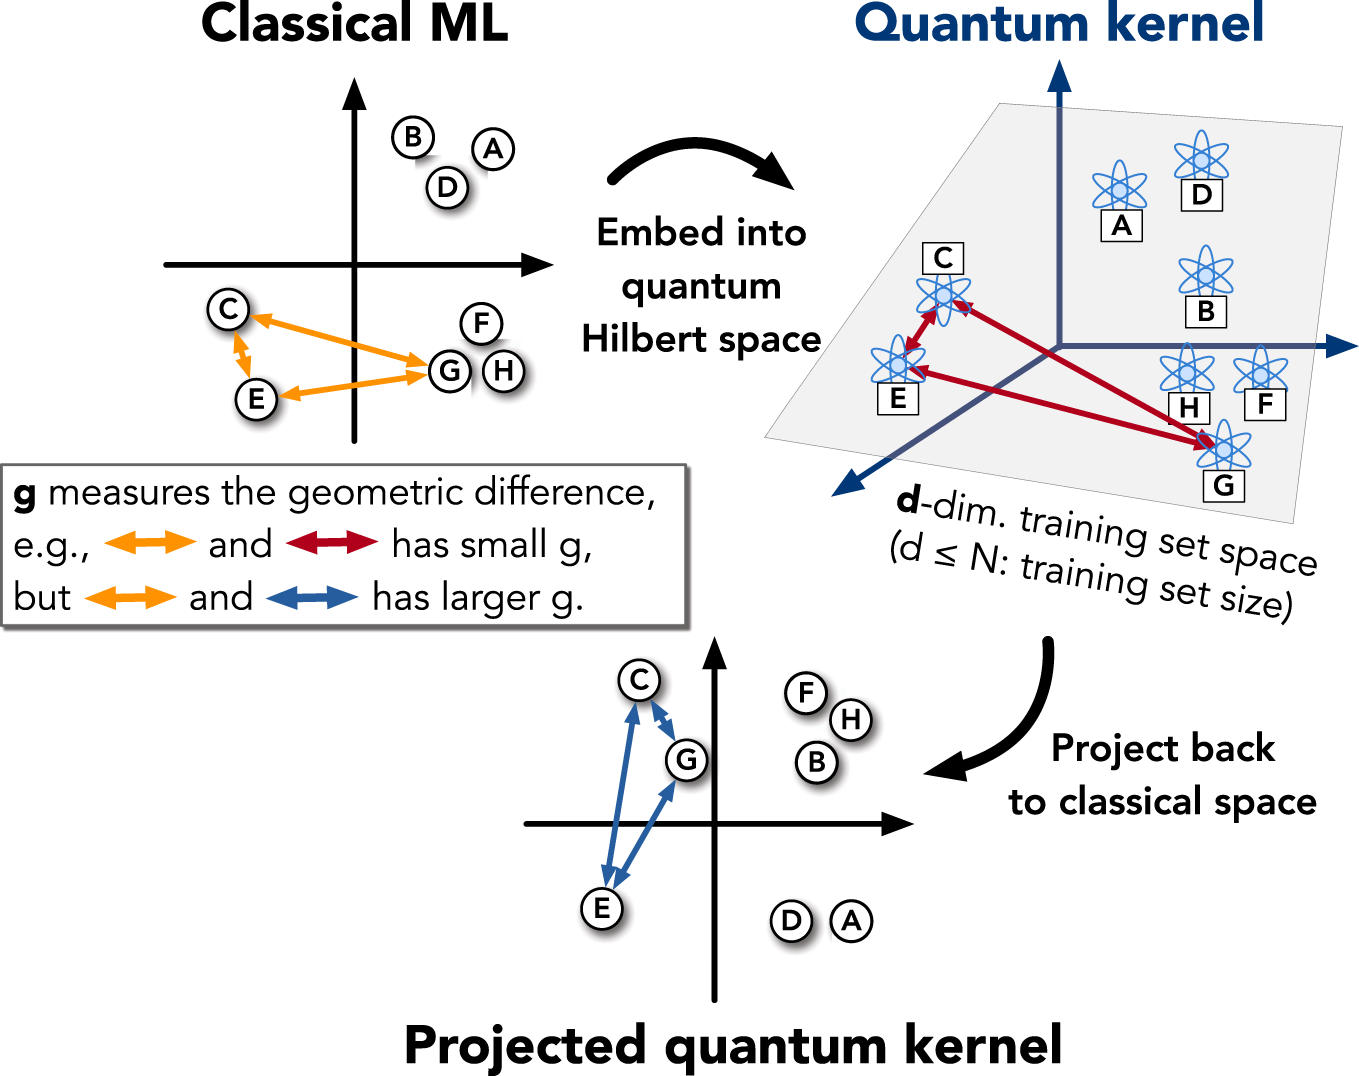
\includegraphics[width=0.7\textwidth]{Figures/Huang2021_Fig2.png}
  \caption{Geometría (función kernel) definida por modelos clásicos y cuánticos. Las letras
  representan datos y las flechas, la similitud entre ellos; la \textit{geometric difference}
  \(g\) mide cuánto difieren esas similitudes entre modelos, y \(d\) es la dimensión efectiva
  del conjunto de entrenamiento en el espacio de Hilbert. Reproducida de Huang et al. (2021),
  \textit{Nat. Commun.} 12, 2631, bajo licencia CC BY 4.0 (\protect\url{https://creativecommons.org/licenses/by/4.0/}).}
  \label{fig:huang_geometria}
\end{figure}

\textbf{Concentración exponencial del kernel cuántico.}
Un obstáculo para escalar de clasificadores cuánticos basados en producto interno
es el fenómeno de concentración, advertido por Huang et al. (``\textit{all inputs are too far apart}'')
y formalizado por Thanasilp et al. \cite{Thanasilp2024}. A medida que el número de qubits $n$
crece, las fidelidades cuánticas fuera de la diagonal
$|\langle\phi(\mathbf{x})|\phi(\mathbf{x}')\rangle|^2$ se concentran exponencialmente en $n$ alrededor de un valor fijo, que para el kernel de fidelidad
es cercano a cero. El kernel se acerca entonces a la matriz identidad, $K_Q \approx I$: todas las
muestras parecen casi ortogonales entre sí y se pierde la noción de vecindad.
Thanasilp et al. identifican cuatro fuentes de concentración: la expresividad del \textit{embedding},
las mediciones globales (como el proyector $|0\dots 0\rangle\langle 0\dots 0|$ con que se estima el kernel
de fidelidad), el entrelazamiento y el ruido. Los
resultados empíricos sobre la concentración observada en este proyecto se presentan en la sección de resultados.

% ---
% Subsección nueva en Docs/Technical_Report.tex
% Decisiones: D-033, H-038, H-039
% ---

\subsubsection{Dimensión efectiva}
\label{sec:dimension_efectiva}

Para caracterizar la expresividad y la estructura espectral de la matriz de kernel sin
depender de las etiquetas de clase, Huang et al. \cite{huang2021power} propusieron el concepto
de \textit{dimensión efectiva} $d(K)$. Esta métrica cuantifica cuántas direcciones
independientes u ortogonales explora el conjunto de datos en el espacio de Hilbert inducido
por el kernel.

Sea $K \in \mathbb{R}^{N \times N}$ una matriz de kernel normalizada a traza $N$
($\operatorname{Tr}(K) = N$). Sean $t_1 \ge t_2 \ge \dots \ge t_N \ge 0$ los autovalores
ordenados de forma decreciente de $K$. La dimensión efectiva se define como:
\begin{equation}
  d(K) = \sum_{k=1}^{N} \frac{1}{N - k + 1}\sum_{l=k}^{N} t_l.
  \label{eq:dim_efectiva}
\end{equation}
En la ecuación~\eqref{eq:dim_efectiva}, el término interior $\sum_{l=k}^{N} t_l$ representa
la suma de la cola espectral a partir del $k$-ésimo autovalor, y el denominador
la promedia entre las $N-k+1$ direcciones restantes.

% respaldo: «In the numerical experiment, we choose the following measure as the approximate dimension» (huang2021powerSupp, p. 12)
% La errata está igual en la versión publicada (S64) y en la de arXiv (F12), sección 6 B = Apéndice F.2.
\textbf{Nota sobre errata en la literatura:} La ecuación (S64) de la información suplementaria de Huang et al. \cite{huang2021power} (sección~6\,B) imprime el factor normalizador como $\frac{1}{N - k}$, formulación que incurre en una indeterminación por división entre cero en el último sumando ($k = N$). La corrección consiste en emplear el denominador $N - k + 1$. Con esta formulación, la métrica satisface las cotas que enuncian los autores:
\begin{equation}
  1 \le d(K) \le N.
  \label{eq:effective_dim_bounds}
\end{equation}
Los dos extremos se comprueban directamente:
\begin{itemize}
  \item \textbf{Cota inferior ($d = 1$):} Si todas las muestras mapean al mismo estado cuántico, la matriz de kernel tiene rango 1 ($t_1 = N$ y $t_l = 0$ para $l \ge 2$). La suma total colapsa a $d = \frac{1}{N} t_1 = \frac{N}{N} = 1$.
  \item \textbf{Cota superior ($d = N$):} Si todas las muestras mapean a estados mutuamente ortogonales en el espacio de Hilbert ($K = I$, autovalores $t_l = 1$ para todo $l$), la cola espectral para cada índice $k$ satisface $\sum_{l=k}^N 1 = N - k + 1$. Al cancelarse con el denominador, cada sumando vale idénticamente 1, resultando en $d = \sum_{k=1}^N 1 = N$.
\end{itemize}

Valores de $d$ cercanos a $N$ indican que cada lesión ocupa casi su propia dirección, como ocurre con un kernel concentrado; valores pequeños, que el kernel agrupa las lesiones en pocas direcciones.

% ---
% Reemplaza líneas 1803-1844 de Docs/Technical_Report.tex
% Decisiones: D-016, D-033
% ---

\subsubsection{Índice Davies-Bouldin}

El índice Davies-Bouldin (DB) \cite{davies1979cluster}
mide la calidad de la separación entre clusters en un
espacio de representación, combinando la dispersión
intra-clase con la separación inter-clase. Para el
problema de clasificación binaria (benigno / maligno),
las dos clases diagnósticas se definen como clusters
predeterminados ($C = 2$). El índice se define como:

\begin{equation}
  \text{DB} =
  \frac{1}{C}\sum_{i=1}^{C}
  \max_{j \neq i}
  \left\{
  \frac{s_i + s_j}{d(c_i, c_j)}
  \right\}
  \label{eq:davies_bouldin}
\end{equation}

\noindent donde $C = 2$ es el número de clases,
$s_i$ es la dispersión promedio de los puntos de la
clase $i$ respecto a su centroide $c_i$:

\begin{equation}
  s_i = \frac{1}{|C_i|}
  \sum_{\mathbf{z} \in C_i}
  \|\mathbf{z} - c_i\|_2
  \label{eq:dispersion}
\end{equation}

\noindent y $d(c_i, c_j) = \|c_i - c_j\|_2$ es la
distancia euclidiana entre los centroides de las clases
$i$ y $j$. Valores bajos del índice DB indican clusters
compactos y bien separados; el valor óptimo es 0.
Esta métrica es independiente del clasificador y puede
aplicarse directamente sobre el vector de embeddings
$\mathbf{e}(\mathbf{x}, \boldsymbol{\theta})$ de las
condiciones cuánticas o sobre los vectores transformados
de las condiciones clásicas. Al depender de distancias
euclidianas invariantes ante rotaciones ortogonales,
el índice DB genera el mismo valor para C1 y C2.

% ---
% Reemplaza líneas 1845-1883 de Docs/Technical_Report.tex
% Decisiones: D-016, D-033
% ---

\subsubsection{Razón multivariante de Fisher}

La razón de Fisher cuantifica la separabilidad lineal entre dos clases comparando la
distancia entre sus centroides frente a la dispersión intraclase. En el análisis univariado
clásico introducido por Fisher \cite{fisher1936use}, el coeficiente mide la separación a lo
largo de un único eje. Sin embargo, en un espacio de representación multivariado $\mathbb{R}^k$
(como el espacio de $k = 12$ dimensiones de los embeddings cuánticos o de las características
radiómicas), la formulación unidimensional promediada coordenada por coordenada ignora las
covarianzas entre variables y adolece de una limitación geométrica: no es invariante
ante transformaciones de rotación.

Para garantizar consistencia metodológica, en este trabajo se adopta la
\textit{razón multivariante de Fisher} (distancia de Mahalanobis al cuadrado entre medias de
clase con la matriz de covarianza combinada):
\begin{equation}
  J = \Delta\boldsymbol{\mu}^\top S_W^{-1} \Delta\boldsymbol{\mu},
  \label{eq:fisher_multivariate}
\end{equation}
donde $\Delta\boldsymbol{\mu} = \boldsymbol{\mu}_1 - \boldsymbol{\mu}_0$ denota el vector de
diferencia entre los centroides de las clases maligna y benigna en $\mathbb{R}^k$, y $S_W$ es
la matriz de dispersión intraclase combinada (\textit{pooled within-class covariance}):
\begin{equation}
  S_W = \frac{1}{N - 2} \left[ \sum_{i \in \mathcal{C}_0} (\mathbf{e}_i - \boldsymbol{\mu}_0)(\mathbf{e}_i - \boldsymbol{\mu}_0)^\top + \sum_{j \in \mathcal{C}_1} (\mathbf{e}_j - \boldsymbol{\mu}_1)(\mathbf{e}_j - \boldsymbol{\mu}_1)^\top \right].
  \label{eq:pooled_covariance}
\end{equation}
La formulación matricial de la ecuación~\eqref{eq:fisher_multivariate} posee una propiedad
algebraica relevante: es invariante ante cualquier transformación afín
invertible del espacio de características, $\mathbf{e} \mapsto A\mathbf{e} + \mathbf{b}$,
con $A \in \mathbb{R}^{k \times k}$ y $\det(A) \neq 0$:
\begin{align}
  J(A\mathbf{e} + \mathbf{b}) &= (A\Delta\boldsymbol{\mu})^\top (A S_W A^\top)^{-1} (A\Delta\boldsymbol{\mu}) \nonumber \\
  &= \Delta\boldsymbol{\mu}^\top A^\top (A^\top)^{-1} S_W^{-1} A^{-1} A \Delta\boldsymbol{\mu} \nonumber \\
  &= \Delta\boldsymbol{\mu}^\top S_W^{-1} \Delta\boldsymbol{\mu} = J(\mathbf{e}).
  \label{eq:fisher_affine_invariance}
\end{align}
Esta invariancia afín es necesaria para el diseño experimental del proyecto. La condición
C2 aplica una transformación por Componentes Principales completa sin reducción de dimensión
($k \to k$). Dicha proyección es una traslación seguida de una rotación ($A \in \mathrm{O}(k)$),
por lo que, bajo la formulación multivariante, se cumple necesariamente que
$J(\text{C1}) = J(\text{C2})$ por construcción.

% ---
% Reemplaza líneas 1884-1906 de Docs/Technical_Report.tex
% Decisiones: D-033
% ---

\subsubsection{Visualización \textit{t-SNE}}

El algoritmo \textit{t-Distributed Stochastic Neighbor
Embedding} (t-SNE) \cite{vandermaaten2008tsne} proyecta
vectores de alta dimensionalidad a un espacio de dos
dimensiones preservando la estructura de vecindad local.
Se utiliza como herramienta de visualización cualitativa
de la separabilidad de clases en el espacio de embeddings:
si la proyección t-SNE muestra clusters compactos y bien
separados por clase, el espacio de representación tiene
estructura discriminativa.

Como complemento visual de las métricas de separabilidad del espacio de embeddings
(DB, Fisher multivariante y KTA lineal), t-SNE se emplea como herramienta de exploración cualitativa.
Para garantizar reproducibilidad, la proyección bidimensional se genera fijando
perplejidad 30, inicialización determinista basada en las dos primeras componentes principales
(PCA) y semilla aleatoria 42 (\texttt{sklearn.manifold.TSNE}). Se utiliza con fines
de soporte visual y no como criterio numérico de decisión.

% ---
% Reemplaza líneas 1907-1967 de Docs/Technical_Report.tex
% Decisiones: D-018, D-036
% ---

\subsubsection{Métricas de clasificación}

El desempeño del clasificador MLP sobre cada condición experimental se evalúa a partir de
las predicciones de probabilidad de malignidad $\hat{y} \in [0, 1]$ generadas por la función
sigmoide de salida. Para las métricas dependientes de umbral, se adopta el umbral de decisión
operativo estándar de 0.5 ($\hat{y} \geq 0.5 \implies \text{maligno}$):

\textbf{Exactitud (\textit{Accuracy}):}
\begin{equation}
  \text{Acc} =
  \frac{TP + TN}{TP + TN + FP + FN}
  \label{eq:accuracy}
\end{equation}

\textbf{Precisión (\textit{Precision}):}
\begin{equation}
  \text{Prec} =
  \frac{TP}{TP + FP}
  \label{eq:precision}
\end{equation}

\textbf{Exhaustividad (\textit{Recall}):}
\begin{equation}
  \text{Rec} =
  \frac{TP}{TP + FN}
  \label{eq:recall}
\end{equation}

\textbf{F1-Score:}
\begin{equation}
  F_1 =
  \frac{2 \cdot \text{Prec} \cdot \text{Rec}}
  {\text{Prec} + \text{Rec}}
  \label{eq:f1}
\end{equation}

\textbf{Área bajo la curva ROC (AUC-ROC):}
\begin{equation}
  \text{AUC} =
  \int_0^1 \text{TPR}(t)\,d\,\text{FPR}(t)
  \label{eq:auc_roc}
\end{equation}

\noindent donde $TP$, $TN$, $FP$ y $FN$ son los
verdaderos positivos, verdaderos negativos, falsos
positivos y falsos negativos respectivamente;
$\text{TPR}(t) = TP/(TP+FN)$ es la tasa de verdaderos
positivos y $\text{FPR}(t) = FP/(FP+TN)$ es la tasa
de falsos positivos, ambas evaluadas al umbral de
decisión $t$.

El \textbf{Área bajo la curva ROC (AUC-ROC)}, formalizada en la ecuación~\eqref{eq:auc_roc},
constituye la métrica principal de comparación técnica entre condiciones. Al integrar la
tasa de verdaderos positivos en función de la tasa de falsos positivos sobre la totalidad de
los umbrales posibles $t \in [0, 1]$, el AUC-ROC cuantifica la capacidad discriminativa intrínseca
del modelo con independencia del umbral operativo y de forma robusta frente al desbalance
de clases del CBIS-DDSM.

El protocolo de validación evalúa todas las métricas mediante validación cruzada de 5 \textit{folds}
estratificada por clase y agrupada por paciente sobre el conjunto de entrenamiento, así
como mediante una evaluación final sobre el conjunto de prueba oficial, que se usa una sola vez por modelo, reportando
intervalos de confianza al 95\,\% derivados de 2\,000 remuestreos \textit{bootstrap} pareados por
paciente.

% ---
% Reemplaza líneas 1968-2007 de Docs/Technical_Report.tex
% Decisiones: D-016, D-039, H-049
% ---

\subsubsection{Análisis de correlación separabilidad--clasificación}

Para dar cumplimiento al objetivo específico OE-5, se evalúa si la jerarquía de separabilidad
geométrica observada en el espacio de representación predice el desempeño predictivo alcanzado
por el clasificador MLP. Para cuantificar la concordancia monótona entre los ordenamientos de las
cinco condiciones experimentales (C1 a C5), se calcula el coeficiente de correlación de rangos
de Spearman $\rho_s$.

La fórmula $1-6\sum d_i^2/(n(n^2-1))$ solo vale sin empates. En el diseño metodológico del presente trabajo,
las condiciones C1 y C2 arrojan idénticos valores de separabilidad por construcción matemática
(invariancia rotacional de Davies-Bouldin, Fisher multivariante y KTA lineal). Al asignarse
rangos promedio a las condiciones empatadas, las sumas de cuadrados de los rangos disminuyen
respecto al caso de rangos discretos enteros, lo que invalida la fórmula de diferencias
cuadráticas. La definición de $\rho_s$, adoptada en este trabajo, corresponde a
la \textit{correlación de Pearson evaluada sobre los rangos promedio}:
\begin{equation}
  \rho_s = \frac{\sum_{i=1}^{n} (R_i - \bar{R})(S_i - \bar{S})}{\sqrt{\sum_{i=1}^{n} (R_i - \bar{R})^2 \sum_{i=1}^{n} (S_i - \bar{S})^2}},
  \label{eq:spearman}
\end{equation}
donde $R_i$ representa el rango asignado a la condición $i$ según la métrica de separabilidad, $S_i$
denota el rango de la condición según el AUC-ROC de clasificación, y $\bar{R} = \bar{S} = \frac{n+1}{2} = 3$
es la media teórica de los rangos para $n = 5$ condiciones. A las condiciones C1 y C2 se les asigna
el rango medio compartido correspondiente a las posiciones que ocupan conjuntamente.

Debido al tamaño reducido del conjunto de condiciones ($n = 5$), el espacio muestral de posibles
permutaciones consta de exactamente $5! = 120$ órdenes posibles, todos equiprobables bajo la hipótesis
nula de ordenamiento aleatorio. En este régimen de muestra pequeña, las aproximaciones asintóticas
estándar (como la distribución $t$ de Student) carecen de validez, y la distribución nula exacta es
discreta:
\begin{itemize}
  \item sin empates, solo $\rho_s=\pm1$ llega a $p<0.05$ bilateral, $p = 2/120 \approx 0.017$, y una sola inversión de vecinos da $\rho_s = 0.9$ con $p = 10/120 \approx 0.083$;
  \item con el empate C1 = C2, el máximo es $\rho_s=\sqrt{19/20}\approx0.975$, alcanzado por 2 de los 120 órdenes, con $p$ bilateral $= 4/120 \approx 0.033$.
\end{itemize}
Por esta razón, el coeficiente de Spearman entre separabilidad y clasificación se reporta con
carácter descriptivo por subproblema (masas y calcificaciones), complementado con su
distribución nula exacta tabulada, evaluando cualitativamente si las
tres condiciones clásicas (C1, C2, C3) se posicionan sistemáticamente por encima de las dos
cuánticas (C4, C5) tanto en separabilidad como en desempeño clasificatorio.

\newpage

% ===== Capítulo: 4_EDA
\setcounter{section}{3}
% ---
% Reemplaza líneas 2924–2940 de Docs/Technical_Report.tex.
% Decisiones que lo respaldan: H-001, H-010, D-012.
% Capítulo 4 desde el 2026-10-14 (antes §5).
% ---

\newpage
\section{Análisis Exploratorio de Datos}
\label{sec:eda}

% fuente: H-001, H-010, D-012
El presente capítulo aborda la caracterización cuantitativa y técnica
del conjunto de datos CBIS-DDSM (\textit{Curated Breast Imaging Subset of
DDSM}), procesando de manera unificada sus cuatro archivos de metadatos
clínicos y enlazándolos con los 3\,568 estudios mamográficos en formato
DICOM disponibles en disco (recuperados íntegramente tras solventar la
omisión de 84 series mediante la API REST de TCIA).

Lejos de constituir un ejercicio meramente descriptivo, este análisis
exploratorio actúa como el puente empírico fundamental que justifica
y condiciona de forma directa las decisiones de diseño del pipeline
experimental desarrollado en el capítulo~\ref{sec:metodologia}. En
particular, la exploración busca dar respuesta a tres interrogantes
estructurales:
\begin{enumerate}
  \item \textbf{Estructura y balance de clases:} ¿Cuál es el grado de
        asimetría diagnóstica entre benignidad y malignidad en cada
        subconjunto, y qué esquemas de ponderación o métricas de
        evaluación exige dicha distribución?
  \item \textbf{Relevancia de los metadatos clínicos frente a la imagen:}
        ¿Aportan las variables categóricas y ordinales registradas
        (densidad mamaria, sutileza, lateralidad o evaluación BI-RADS)
        señal predictiva utilizable, o debe extraerse la información
        discriminativa directamente del tejido tisular en la imagen?
  \item \textbf{Factibilidad y restricciones de la representación cuántica:}
        ¿Qué características técnicas (resolución espacial, rango dinámico,
        profundidad de bits, alineación de máscaras de contorno y
        ausencia de espaciado físico de píxel) delimitan la viabilidad
        de codificar la información en estados cuánticos de pocos qubits?
\end{enumerate}

El capítulo se estructura en cuatro bloques temáticos: saneamiento y
validación del dataset, análisis de la variable patológica objetivo,
evaluación de correlaciones en variables clínicas, e inspección técnica
de las imágenes DICOM. Finalmente, se sintetizan las implicaciones
directas que estos hallazgos imponen sobre cada módulo de la metodología.
Todos los procedimientos y figuras analíticas descritos en este capítulo
fueron ejecutados en el cuaderno \texttt{1\_EDA.ipynb} del repositorio.

% ---
% Reemplaza líneas 2941–2996 de Docs/Technical_Report.tex.
% Decisiones que lo respaldan: D-005, D-012, H-001.
% Capítulo 4 desde el 2026-10-14 (antes §5).
% ---

\subsection{Validación y limpieza de los datos}

% fuente: H-001, D-005
La carga y unificación de los cuatro archivos CSV produjo
un DataFrame consolidado de 3\,568 registros, con las
columnas \texttt{finding\_type} (masa / calcificación) y
\texttt{split} (train / test) agregadas para facilitar
el análisis por subconjunto. La Tabla~\ref{tab:eda_resumen}
presenta el resumen de la composición del dataset.

% fuente: H-001, D-005, H-038
\begin{table}[htbp]
\centering
\caption{Composición del dataset CBIS-DDSM unificado}
\label{tab:eda_resumen}
\renewcommand{\arraystretch}{1.3}
\begin{tabularx}{\textwidth}{@{}Xrr@{}}
\toprule
\textbf{Subconjunto} &
\textbf{Train} & \textbf{Test} \\
\midrule
Masas (mass)           & 1\,318 & 378 \\
Calcificaciones (calc) & 1\,546 & 326 \\
\midrule
\textbf{Total}         & \textbf{2\,864} &
                         \textbf{704} \\
\bottomrule
\end{tabularx}
\end{table}

% fuente: D-005, H-001; 1_EDA.ipynb
La etiqueta objetivo \texttt{pathology} presentó tres
valores distintos en los datos originales:
\texttt{BENIGN} (1\,548 casos),
\texttt{MALIGNANT} (1\,457 casos) y
\texttt{BENIGN\_WITHOUT\_CALLBACK} (563 casos).
Los casos \texttt{BENIGN\_WITHOUT\_CALLBACK} fueron
normalizados a \texttt{BENIGN} por equivalencia clínica,
resultando en la codificación binaria
0\,=\,benigno (2\,111 casos, 59.2\,\%) y
1\,=\,maligno (1\,457 casos, 40.8\,\%).

La validación de nulos confirmó que las columnas
\texttt{mass\_shape}, \texttt{mass\_margins},
\texttt{calc\_type} y \texttt{calc\_distribution}
presentan valores faltantes de naturaleza estructural:
los registros de calcificaciones no tienen valores en
las columnas de masas y viceversa, por diseño del
dataset. No se identificaron errores de datos que
requirieran corrección.

% fuente: D-012, H-001
La verificación del enlace entre registros CSV y
archivos DICOM en disco arrojó una cobertura del
100\,\% (3\,568/3\,568 registros con archivo
DICOM encontrado), alcanzada tras recuperar las 84 series
faltantes mediante la API REST de TCIA; la descarga inicial
con el NBIA Data Retriever dejaba una cobertura del 97.6\,\%.

% ---
% Reemplaza líneas 2997–3096 de Docs/Technical_Report.tex.
% Decisiones que lo respaldan: D-005, H-050.
% Capítulo 4 desde el 2026-10-14 (antes §5).
% ---

\subsection{Análisis de la variable objetivo}

\subsubsection{Distribución de clases y balance}

La distribución de la variable objetivo a nivel global, por tipo de
hallazgo y por partición de entrenamiento y prueba (\textit{train/test})
se ilustra en la Figura~\ref{fig:class_distribution} del
Anexo~\ref{anx:figuras_eda}.

% fuente: D-005; 1_EDA.ipynb
El dataset presenta un desbalance global moderado de
1.45:1 (benigno/maligno), que se distribuye de forma
heterogénea entre los dos tipos de hallazgo.
La Figura~\ref{fig:imbalance_by_finding} ilustra
esta asimetría mediante gráficas de pastel por
subconjunto.

\begin{figure}[htbp]
  \centering
  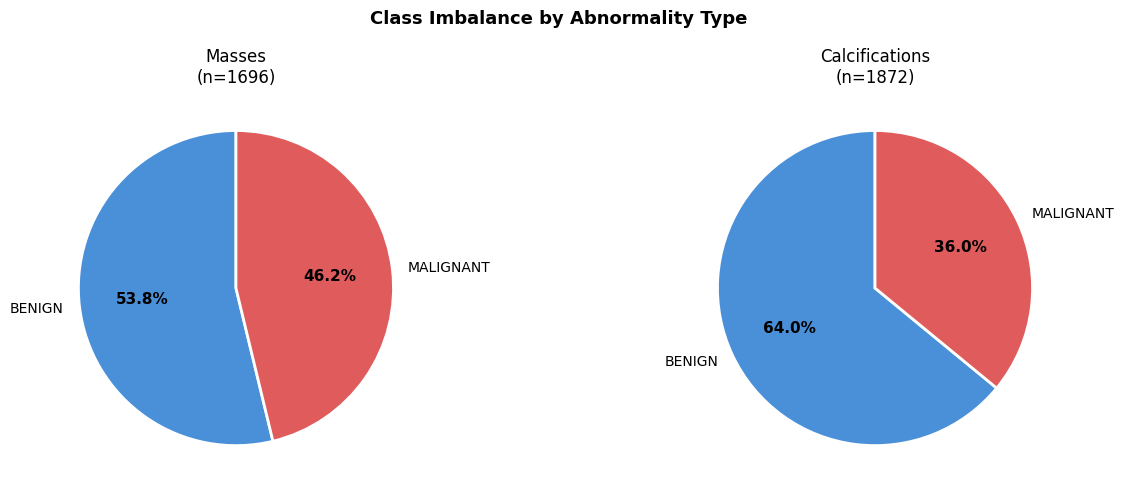
\includegraphics[width=0.75\textwidth]{Figures/B2_imbalance_by_finding.png}
  \caption{Desbalance de clases por tipo de hallazgo.}
  \label{fig:imbalance_by_finding}
\end{figure}

% fuente: D-005; 1_EDA.ipynb
Las masas presentan un balance casi simétrico (ratio
1.16:1), con 912 casos benignos y 784 malignos.
Las calcificaciones muestran un desbalance más
pronunciado (ratio 1.78:1), con 1\,199 casos benignos
frente a 673 malignos. Esta asimetría tiene una
implicación metodológica directa: se requiere
ponderación de clases (\texttt{class\_weight=balanced})
durante el entrenamiento del MLP, aplicada de forma
independiente para cada subconjunto, como se
especifica en el requerimiento RF-19.

\subsubsection{Distribución BI-RADS}

La distribución detallada de la categoría BI-RADS por patología
y tipo de hallazgo se presenta en la Figura~\ref{fig:birads_distribution}
del Anexo~\ref{anx:figuras_eda}.

% fuente: D-005; 1_EDA.ipynb
Se observa una concentración de casos malignos en las
categorías BI-RADS 4 y 5 (sospechoso y altamente
sospechoso), mientras que los casos benignos se
distribuyen predominantemente en las categorías 2 y
3. Esta distribución valida la coherencia clínica del
dataset: la categoría BI-RADS refleja directamente
el nivel de sospecha de malignidad asignado por el
radiólogo.

\subsubsection{Análisis de subtlety}

% fuente: D-005; 1_EDA.ipynb
La distribución de sutileza visual (\textit{subtlety}) por patología
y tipo de hallazgo se recoge en la Figura~\ref{fig:subtlety_distribution}
del Anexo~\ref{anx:figuras_eda}.

% fuente: 1_EDA.ipynb (celda «SUBTLETY POR PATOLOGIA»); Data/cbis_ddsm_unified.csv.
% Corregido el 2026-10-19 (auditoría A2-1): TT1 daba 3.1/2.8 frente a 3.4/3.2, cifras que no
% salen de los datos, y en masas el sentido estaba invertido.
La media de \textit{subtlety} en casos malignos es
ligeramente mayor que en benignos en masas (3.98 frente
a 3.88) y ligeramente menor en calcificaciones (3.23
frente a 3.49), con la misma mediana dentro de cada
subconjunto (4 en masas y 3 en calcificaciones). En
ambos casos la diferencia es pequeña.
Este hallazgo no respalda la intuición de que las lesiones
malignas son necesariamente más difíciles de detectar
visualmente: la dificultad de detección es
aproximadamente ortogonal a la patología, lo que
explica parcialmente por qué los modelos de deep
learning enfrentan dificultades de generalización al
no poder apoyarse en la obviedad visual como señal
discriminativa.

% ---
% Reemplaza líneas 3097–3252 de Docs/Technical_Report.tex.
% Decisiones que lo respaldan: D-005, D-006, H-050.
% Capítulo 4 desde el 2026-10-14 (antes §5).
% ---

\subsection{Análisis de variables clínicas}

\subsubsection{Densidad mamaria}

La distribución de densidad mamaria clasificada por el radiólogo
según patología y tipo de hallazgo se ilustra en la
Figura~\ref{fig:breast_density} del Anexo~\ref{anx:figuras_eda}.

% fuente: D-005; 1_EDA.ipynb
La densidad mamaria más frecuente en el dataset es
la categoría 2 (tejido disperso). El análisis de
correlación confirmó que la densidad mamaria tiene
una correlación casi nula con la etiqueta de
patología ($r = -0.03$ para masas, $r = +0.09$ para
calcificaciones), lo que indica que la densidad
no predice la malignidad de la lesión. Sin embargo,
se observó una correlación negativa moderada entre
densidad y \textit{subtlety} ($r = -0.31$ para masas),
confirmando que las lesiones son más difíciles de
detectar visualmente en tejidos más densos, donde
el tejido glandular camufla las estructuras anómalas.

\subsubsection{Lateralidad y vista mamográfica}

La distribución de lateralidad anatómica y proyección mamográfica
se presenta en la Figura~\ref{fig:laterality_view} del
Anexo~\ref{anx:figuras_eda}.

% fuente: D-005; 1_EDA.ipynb
La distribución de lateralidad es prácticamente
simétrica (1\,819 casos izquierdos vs.\ 1\,749
derechos, ratio 1.04:1), lo que indica ausencia de
sesgo de adquisición por lado. El ligero predominio
de la vista MLO sobre la CC (1\,896 vs.\ 1\,672)
es esperado clínicamente, dado que la vista
MLO captura mayor volumen de tejido mamario
incluyendo la región axilar.

\subsubsection{Morfología de masas}

La Figura~\ref{fig:mass_morphology} muestra la
distribución de forma y margen de las masas por
patología.

\begin{figure}[htbp]
  \centering
  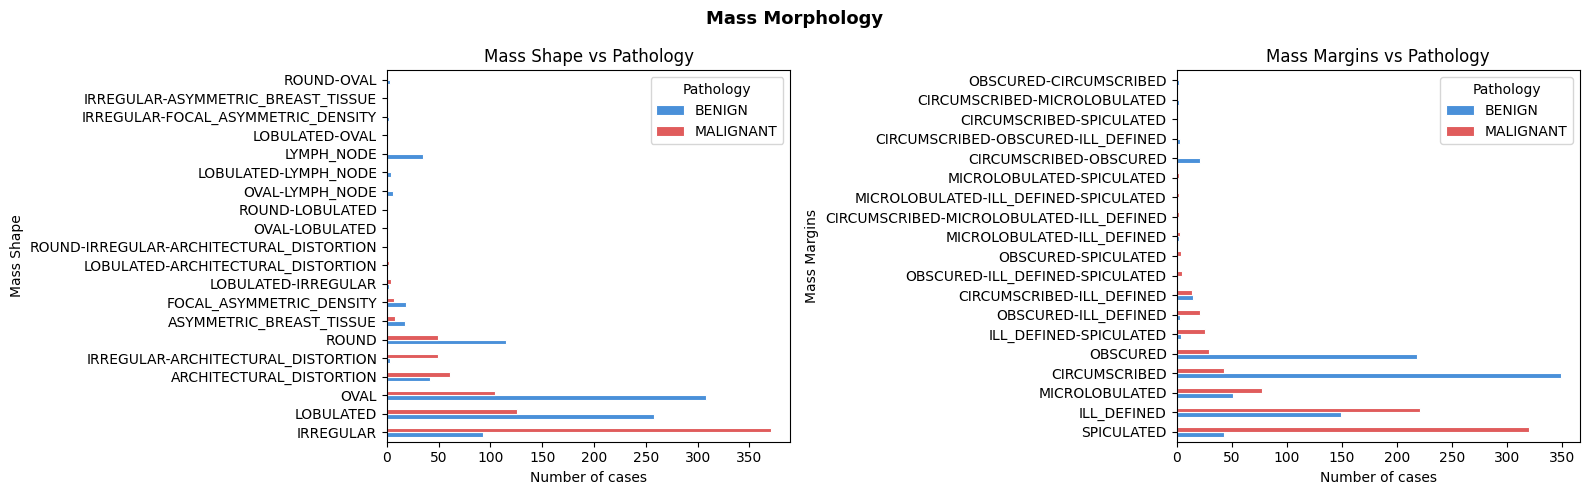
\includegraphics[width=\textwidth]{Figures/C3_mass_morphology.png}
  \caption{Distribución de forma y margen de masas por patología (benigno / maligno).}
  \label{fig:mass_morphology}
\end{figure}

Los resultados revelan una separación morfológica
marcada entre clases. Las masas malignas se asocian
predominantemente con formas \textit{IRREGULAR} y
márgenes \textit{SPICULATED}, patrón clínico clásico
del carcinoma invasivo, donde el tumor crece
desordenadamente con extensiones hacia el tejido
circundante. Las masas benignas presentan formas
\textit{OVAL} con bordes \textit{CIRCUMSCRIBED},
patrón típico de fibroadenomas o quistes encapsulados.
Esta separación morfológica sugiere que las
características extraídas de masas deberían ser
intrínsecamente más separables en cualquier espacio
de representación, incluyendo el espacio de Hilbert
cuántico generado por los \textit{feature maps}.

\subsubsection{Morfología de calcificaciones}

La Figura~\ref{fig:calc_morphology} presenta la
distribución de tipo y distribución de las
calcificaciones por patología.

\begin{figure}[htbp]
  \centering
  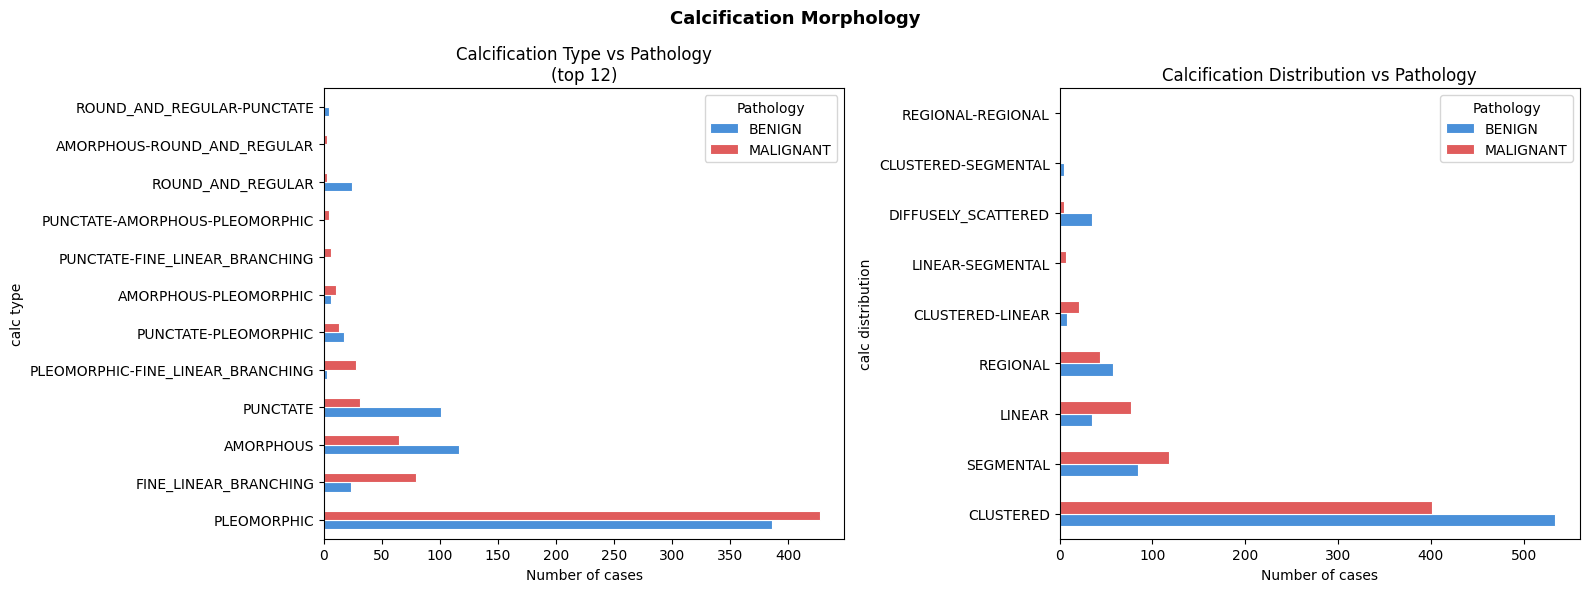
\includegraphics[width=\textwidth]{Figures/C4_calc_morphology.png}
  \caption{Distribución de tipo y distribución espacial de calcificaciones por patología.}
  \label{fig:calc_morphology}
\end{figure}

A diferencia de las masas, las calcificaciones
presentan el tipo morfológico más frecuente
(\textit{PLEOMORPHIC}) compartido entre ambas clases.
Este solapamiento morfológico implica que las
calcificaciones constituyen un problema de
clasificación más exigente que las masas en cuanto a
los descriptores categóricos del radiólogo. Este
escenario es relevante para el presente trabajo
porque permite contrastar el efecto de las
transformaciones cuánticas en dos subproblemas de
dificultad distinta.
% Corregido el 2026-10-19 (auditoría A5-2): el texto de TT1 anticipaba que la codificación cuántica
% «puede revelar estructura discriminativa no accesible para los métodos clásicos», en contradicción
% con §2.1.6 y §6; además, con las 67 características radiómicas las calcificaciones resultan más
% separables que las masas (§6.5), así que la menor separabilidad vale solo para los descriptores.

\subsubsection{Correlaciones entre variables clínicas}

La Figura~\ref{fig:correlation_matrix} presenta la
matriz de correlación de las variables clínicas
numéricas del dataset.

\begin{figure}[htbp]
  \centering
  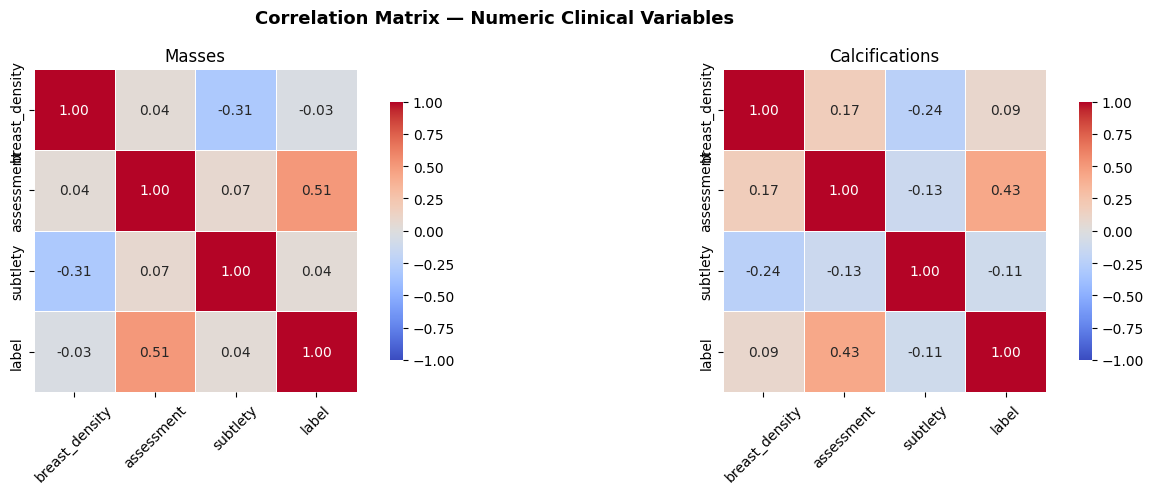
\includegraphics[width=\textwidth]{Figures/C5_correlation_matrix.png}
  \caption{Matriz de correlación de variables clínicas numéricas por tipo de hallazgo.}
  \label{fig:correlation_matrix}
\end{figure}

% fuente: D-005; 1_EDA.ipynb
La variable \texttt{assessment} (categoría BI-RADS)
presenta la correlación más alta con la etiqueta de
patología ($r = +0.51$ para masas, $r = +0.43$ para
calcificaciones), lo cual es esperado dado que el
BI-RADS fue diseñado precisamente como escala de
sospecha de malignidad. Sin embargo, esta variable
no puede utilizarse como \textit{feature} de entrada
al modelo porque constituye \textit{data leakage}:
es una etiqueta clínica derivada de la imagen, no
una característica morfológica independiente.

% fuente: D-005, D-006; 1_EDA.ipynb
Las variables \texttt{breast\_density} y
\texttt{subtlety} presentan correlaciones
prácticamente nulas con la etiqueta de patología
($|r| < 0.12$ en todos los casos), confirmando que
el poder predictivo reside en las características
morfológicas de la imagen y no en los metadatos
clínicos del CSV. Este resultado valida la decisión
metodológica de extraer \textit{features} directamente
de las imágenes DICOM mediante PyRadiomics.

% ---
% Reemplaza líneas 3253–3394 de Docs/Technical_Report.tex.
% Decisiones que lo respaldan: D-006, D-009, D-022, H-002.
% Capítulo 4 desde el 2026-10-14 (antes §5).
% ---

\subsection{Análisis de imágenes DICOM}

\subsubsection{Dimensiones y características técnicas}

La Figura~\ref{fig:image_dimensions} muestra la
distribución de dimensiones de las mamografías
completas en la muestra analizada.

\begin{figure}[htbp]
  \centering
  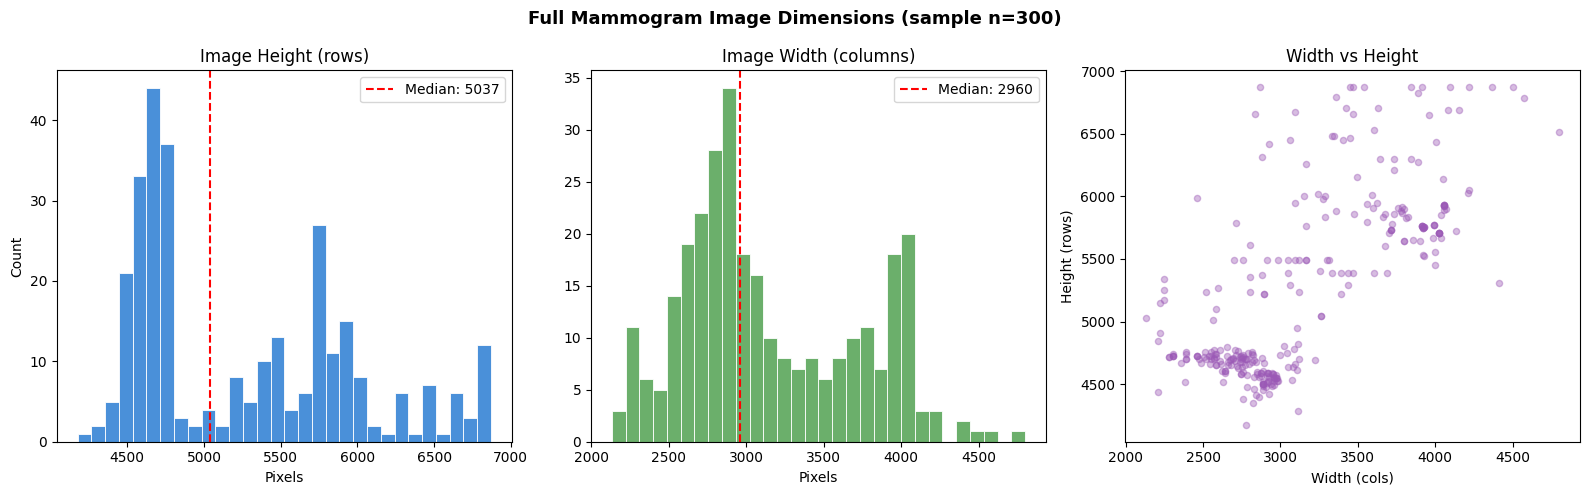
\includegraphics[width=0.8\textwidth]{Figures/D1_image_dimensions.png}
  \caption{Distribución de dimensiones (altura y anchura en píxeles) de las mamografías completas (muestra n\,=\,300).}
  \label{fig:image_dimensions}
\end{figure}

% fuente: D-009; 1_EDA.ipynb
Las mamografías completas presentan dimensiones
medianas de 5\,037\,$\times$\,2\,960 píxeles con
profundidad de 16 bits, lo que confirma que su tamaño
es incompatible con la entrada directa a un circuito
cuántico. Este hallazgo valida la decisión de diseño
de trabajar con recortes de la región de interés a
resolución original, de los que se extraen
características radiómicas (capítulo~\ref{sec:metodologia},
sección~\ref{sec:modulo3}) en lugar de las mamografías completas.

% fuente: H-002; 1_metadatos_dicom.csv
La inspección de los metadatos DICOM reveló que las
imágenes del dataset son de tipo \textit{Secondary
Capture} (\texttt{SOPClassUID}:
1.2.840.10008.5.1.4.1.1.7), generadas mediante
MATLAB (\texttt{SecondaryCapture}\allowbreak\texttt{DeviceManufacturer}:
MathWorks) como parte del proceso de digitalización
y curaduría del CBIS-DDSM. La convención fotométrica
es \texttt{MONOCHROME2} de forma uniforme en todo el
dataset, lo que elimina la necesidad de inversión de
píxeles en el preprocesamiento.

\subsubsection{Variabilidad inter-escáner}

% fuente: H-002; 1_metadatos_dicom.csv
Ninguna de las 3\,103 mamografías distintas incluye las etiquetas
\texttt{Manufacturer}, \texttt{PixelSpacing} ni
\texttt{ImagerPixelSpacing}; las tres faltan en los archivos
DICOM (véase la Figura~\ref{fig:manufacturers} del Anexo~\ref{anx:figuras_eda}).
Como consecuencia, no es posible un análisis de
variabilidad entre escáneres a partir de metadatos, y las
características de forma quedan en píxeles sin escala física;
como el DDSM original se digitalizó con escáneres de distinta
resolución, el mismo tamaño físico da distinto número de
píxeles según el digitalizador, lo que se declara como
limitación. Todas las imágenes corresponden a la modalidad MG,
con profundidad de 16 bits y convención fotométrica
\texttt{MONOCHROME2}.

\subsubsection{Distribución de intensidades de píxeles}

La comparación cuantitativa de las distribuciones estadísticas
de intensidad de píxeles (media, desviación estándar y máximo)
entre casos benignos y malignos en las imágenes de ROI se presenta
en la Figura~\ref{fig:pixel_intensities} del Anexo~\ref{anx:figuras_eda}.

% fuente: D-006, D-022; 1_EDA.ipynb
Las imágenes recortadas presentan valores de
intensidad media en el rango de 45\,000--50\,000
sobre un máximo posible de 65\,535 (16 bits),
con máximos frecuentemente en el límite superior.
Las distribuciones de casos benignos y malignos
muestran solapamiento considerable en las tres
estadísticas analizadas, confirmando que la
información discriminativa no reside en estadísticas
globales de intensidad sino en patrones texturales
y morfológicos de orden superior, que son precisamente
los que capturan las \textit{features} radiómicas
de PyRadiomics.

\subsubsection{Galería de casos representativos}

Una galería visual de casos representativos que ilustra la
mamografía completa, la máscara binaria ROI y la imagen recortada
de la lesión se exhibe en la Figura~\ref{fig:sample_gallery} del
Anexo~\ref{anx:figuras_eda}.

La galería ilustra visualmente las diferencias
morfológicas descritas en el análisis de variables
clínicas: las masas malignas muestran bordes
irregulares y espiculados, mientras que las masas
benignas presentan contornos lisos y bien definidos.
En las calcificaciones, la distinción visual entre
clases es menos evidente, consistente con el hallazgo
de que PLEOMORPHIC es el tipo morfológico más
frecuente en ambas clases.

La Figura~\ref{fig:roi_overlays} muestra la
superposición de la máscara ROI sobre la mamografía
completa para cuatro casos seleccionados.

\begin{figure}[htbp]
  \centering
  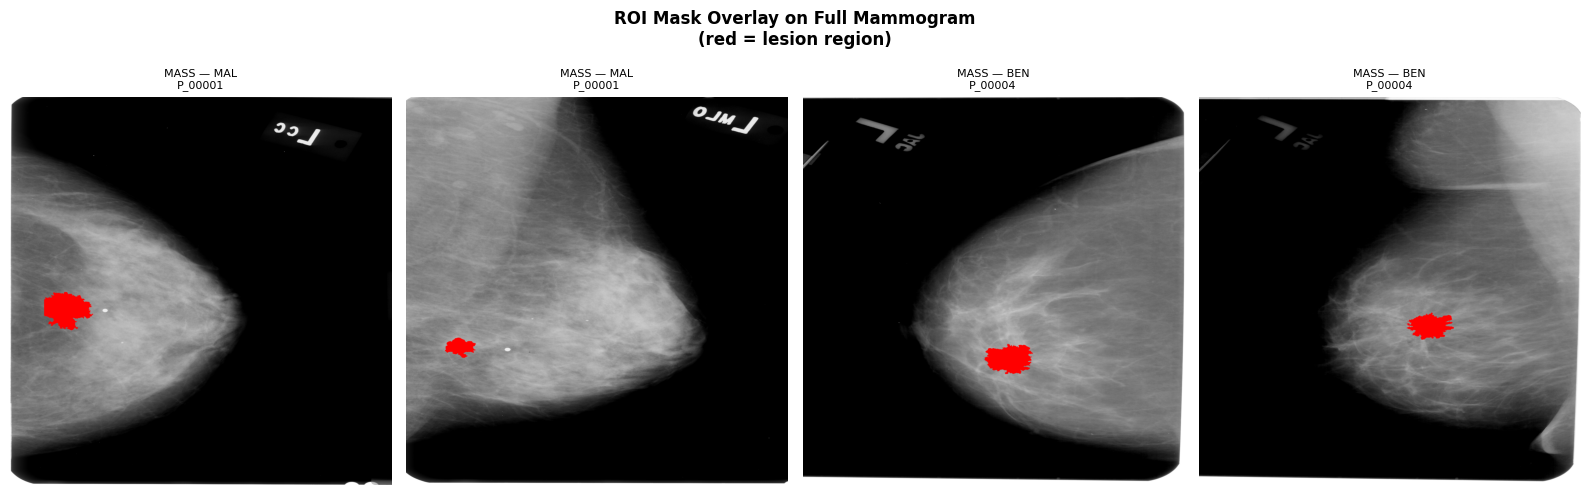
\includegraphics[width=\textwidth]{Figures/D5_roi_overlays.png}
  \caption{Superposición de la máscara ROI (región en rojo) sobre la mamografía completa para cuatro casos representativos.}
  \label{fig:roi_overlays}
\end{figure}

La visualización muestra que las máscaras ROI
delimitan la región de la lesión dentro de la
mamografía completa, lo que respalda su uso como
guía para el recorte. La verificación sistemática
del preprocesamiento encontró 80 máscaras con
dimensiones distintas a las de su mamografía, que
se tratan en la sección~\ref{sec:modulo2}.

% ---
% Reemplaza líneas 3395–3449 de Docs/Technical_Report.tex.
% Decisiones que lo respaldan: D-005, D-006, D-008, D-009, D-011, D-018, D-020, D-021, D-022, D-026, D-036, H-002, H-004, H-005, H-007, H-008, H-020, H-027, H-050, H-051.
% Capítulo 4 desde el 2026-10-14 (antes §5).
% ---

\subsection{Implicaciones para el diseño}
\label{sec:implicaciones_diseno}

El análisis exploratorio de datos permite identificar un conjunto de
hallazgos empíricos y restricciones técnicas que justifican de manera
directa las decisiones de diseño metodológico del pipeline experimental.
A continuación se detallan los hallazgos principales observados:

\begin{enumerate}

% fuente: D-005, RF-19; 1_EDA.ipynb
\item \textbf{Desbalance de clases diferenciado.}
El ratio benigno/maligno presenta un desbalance moderado en masas
y marcadamente superior en calcificaciones. La ponderación de
clases durante el entrenamiento del MLP es necesaria para
calcificaciones pero opcional para masas. Los modelos se evalúan con
AUC-ROC como métrica principal por su robustez ante este desbalance.

% fuente: H-050
\item \textbf{Asimetría de separabilidad esperada.}
Las masas presentan patrones morfológicos claramente diferenciados
entre clases (IRREGULAR/\allowbreak SPICULATED vs.\ OVAL/\allowbreak CIRCUMSCRIBED),
prediciendo mayor separabilidad en el espacio de representación. Las
calcificaciones comparten el tipo morfológico más frecuente (PLEOMORPHIC)
entre ambas clases, prediciendo menor separabilidad y constituyendo el
caso de prueba más exigente para los \textit{quantum embeddings}.

% fuente: D-006
\item \textbf{Variables clínicas no predictivas.}
La densidad mamaria y el \textit{subtlety} tienen correlación
prácticamente nula con la patología. La información discriminativa
reside en los patrones morfológicos de la imagen, validando el uso de
PyRadiomics como extractor de características.

% fuente: D-009, H-051; 1_EDA.ipynb
\item \textbf{Imágenes de alta dimensionalidad.}
Las mamografías completas tienen dimensiones medianas de
5\,037\,$\times$\,2\,960 píxeles, incompatibles con la entrada directa
al circuito cuántico. El trabajo con recortes de la región de interés
a resolución original, seguido de extracción de características
radiómicas y selección de $k$ características, es la estrategia viable
para la simulación cuántica disponible.

% fuente: D-022, H-002; 1_metadatos_dicom.csv
\item \textbf{Convención fotométrica uniforme.}
La totalidad del dataset utiliza \texttt{MONOCHROME2}, eliminando la
necesidad de inversión de píxeles en el preprocesamiento.

\end{enumerate}

En la Tabla~\ref{tab:eda_implicaciones_diseno} se sintetiza el puente
entre cada hallazgo empírico del análisis exploratorio, la decisión de
diseño adoptada y la subsección de la Metodología donde se materializa.

% fuente: D-005, D-006, D-008, D-009, D-011, D-018, D-020, D-021, D-022, D-026, D-036, H-002, H-004, H-005, H-007, H-008, H-020, H-027, H-050, H-051; 1_EDA.ipynb
\begin{table}[htbp]
\centering
\caption{Correspondencia entre hallazgos del EDA y decisiones de diseño del pipeline}
\label{tab:eda_implicaciones_diseno}
\begin{tabularx}{\textwidth}{@{}X X p{3cm}@{}}
\toprule
\textbf{Hallazgo del EDA} & \textbf{Decisión de diseño} & \textbf{Dónde se aplica} \\
\midrule
Masas y calcificaciones con morfología y desbalance distintos &
Tratamiento como subproblemas totalmente independientes a lo largo de todo el pipeline experimental. &
Sec.~\ref{sec:descripcion_general} y M1--M8 \\
Desbalance 1.16:1 en masas y 1.78:1 en calcificaciones &
Ponderación de clases (\texttt{class\_weight=balanced}) en la pérdida de entropía cruzada del MLP. &
Sec.~\ref{sec:modulo7} (M7) \\
\texttt{breast\_density} y \texttt{subtlety} sin correlación con patología &
La señal reside en la imagen: extracción directa de features radiómicas (PyRadiomics), sin metadatos. &
Sec.~\ref{sec:modulo3} (M3) \\
Mamografías completas de $\sim$5\,037$\times$2\,960~px &
Recorte centrado en la ROI a resolución nativa y extracción radiómica; no se ingresa la imagen al circuito. &
Sec.~\ref{sec:modulo2} y~\ref{sec:modulo3} \\
\texttt{PixelSpacing} ausente en todos los DICOM &
Cálculo de features de forma en píxeles sin escala física dimensional (declarado como limitación). &
Sec.~\ref{sec:modulo3} (M3) \\
80 máscaras con dimensiones discrepantes &
Alineación en M2 según tipo: remuestreo para 78 masas escaladas (factor 0.870) y anclaje para 2 casos. &
Sec.~\ref{sec:modulo2} (M2) \\
Todas \texttt{MONOCHROME2}, 16~bits de profundidad &
Sin inversión fotométrica; discretización de histograma mediante \texttt{binCount=32} en PyRadiomics. &
Sec.~\ref{sec:modulo2} y~\ref{sec:modulo3} \\
Estructura agrupada por paciente &
Partición de validación cruzada con folds agrupados por paciente (\texttt{StratifiedGroupKFold}). &
Sec.~\ref{sec:modulo4} (M4) \\
\bottomrule
\end{tabularx}
\end{table}

\newpage

% ===== Capítulo: 5_Metodologia
\setcounter{section}{4}
% ---
% Reemplaza líneas 2008–2024 de Docs/Technical_Report.tex.
% Decisiones que lo respaldan: D-030 (marco metodológico CRISP-DM).
% ---

\newpage
\section{Metodología}
\label{sec:metodologia}

La metodología adoptada en el presente trabajo es
\textbf{CRISP-DM} (\textit{Cross Industry Standard Process
for Data Mining}), adaptada al contexto de cómputo cuántico.
Esta metodología fue seleccionada por proporcionar un flujo
estructurado que permite integrar de forma natural
tanto las etapas clásicas de análisis de datos como las
etapas cuánticas de codificación y transformación,
manteniendo trazabilidad entre los objetivos de negocio
y las decisiones técnicas de implementación.

La correspondencia entre las fases de CRISP-DM y los módulos
del sistema se describe en la
Tabla~\ref{tab:crisp_modulos}, y el diagrama completo del
pipeline se presenta en la
Figura~\ref{fig:pipeline_sistema}.

% ---
% Reemplaza líneas 2026–2231 de Docs/Technical_Report.tex.
% Decisiones que lo respaldan: D-005, D-009, D-013, D-014, D-016, D-017, D-022, D-023, D-024, D-025, D-030, D-031.
% ---

\subsection{Descripción general del proceso}
\label{sec:descripcion_general}

\begin{figure}[H]
\centering
\begin{tikzpicture}[every node/.style={scale=0.7}, node distance=0.5cm and 0.3cm]

\node[blkGray] (ds) {%
  \textbf{CBIS-DDSM Dataset}\\[2pt]
  {\normalfont\scriptsize
  1{,}566 pacientes $\cdot$ 3{,}568 lesiones $\cdot$ DICOM $+$ CSV\\
  masas y calcificaciones como subproblemas independientes}%
};

\node[blkTeal, below=of ds] (m1) {%
  \textbf{M1 $\cdot$ Lectura de datos}\\[2pt]
  {\normalfont\scriptsize
  \texttt{pydicom} $\cdot$ \texttt{pandas} $\cdot$ DICOM + CSV unificados}%
};

\node[blkTeal, below=of m1] (m2) {%
  \textbf{M2 $\cdot$ Preprocesamiento}\\[2pt]
  {\normalfont\scriptsize
  Alineación y limpieza de máscaras $\cdot$
  Recorte ROI a resolución original $\cdot$ intensidades de 16 bits}%
};

\node[blkTeal, below=of m2] (m3) {%
  \textbf{M3 $\cdot$ Extracción de características}\\[2pt]
  {\normalfont\scriptsize
  PyRadiomics: primer orden, forma, GLCM, GLRLM
  $\rightarrow \mathbf{x} \in \mathbb{R}^{67}$}%
};

\node[blkTeal, below=of m3] (m4) {%
  \textbf{M4 $\cdot$ Selección y escalado}\\[2pt]
  {\normalfont\scriptsize
  F-test con restricción $|r| \le 0.95$ ($k = 12$)
  $+$ cuantiles $\rightarrow \mathbf{x} \in [0,\pi]^{12}$}%
};

\node[font=\tiny\color{colGray}, below=0.25cm of m4] (lm5) {%
  M5 $\cdot$ Transformación (5 condiciones experimentales)%
};
\coordinate (fork) at ($(lm5.south) + (0,-0.2cm)$);

\node[cond, anchor=north] at ($(fork) + (-6.2cm, -0.1cm)$) (c1){%
  \textbf{C1 $\cdot$ Sin}\\ \textbf{transf.}\\[4pt]
  {\normalfont\tiny Baseline}\\ {\normalfont\tiny crudo}%
};
\node[cond, anchor=north] at ($(fork) + (-3.1cm, -0.1cm)$) (c2){%
  \textbf{C2 $\cdot$ PCA}\\ \textbf{lineal}\\[4pt]
  {\normalfont\tiny Control}\\ {\normalfont\tiny nulo}%
};
\node[cond, anchor=north] at ($(fork) + (0cm, -0.1cm)$) (c3){%
  \textbf{C3 $\cdot$ Kernel}\\ \textbf{PCA (RBF)}\\[4pt]
  {\normalfont\tiny Baseline}\\ {\normalfont\tiny no lineal}%
};
\node[condQ, anchor=north] at ($(fork) + (3.2cm, -0.1cm)$) (c4){%
  \textbf{C4 $\cdot$ Qiskit}\\ \textit{ZZ feature map}\\[4pt]
  {\normalfont\tiny ansatz con $\theta$ fijo}\\
  {\normalfont\tiny$\langle Z_i\rangle \in [-1,1]^{12}$ $\cdot$ $K_Q$}%
};
\node[condQ, anchor=north] at ($(fork) + (6.3cm, -0.1cm)$) (c5){%
  \textbf{C5 $\cdot$ Qiskit}\\ \textit{Pauli feature map} $(Y, ZZ)$\\[4pt]
  {\normalfont\tiny ansatz con $\theta$ fijo}\\
  {\normalfont\tiny$\langle Z_i\rangle \in [-1,1]^{12}$ $\cdot$ $K_Q$}%
};

%% Convergencia centrada bajo C3 y a la altura de las cajas cuánticas, que son las más altas
\coordinate (merge) at ($(c3.south |- c5.south) + (0,-0.5cm)$);
\coordinate (mergeL) at (merge -| c1);
\coordinate (mergeR) at (merge -| c5);

%% M6 y M7 en paralelo: ambos consumen la salida de M5
\node[blkAmber, anchor=north, text width=5.6cm, minimum height=1.9cm]
  at ($(merge) + (-2.9cm, -0.6cm)$) (m6){%
  \textbf{M6 $\cdot$ Análisis de separabilidad}\\[2pt]
  {\normalfont\scriptsize
  KTA $\cdot$ \textit{geometric difference} $g_{CQ}$ $\cdot$
  Davies-Bouldin $\cdot$ Fisher $\cdot$ t-SNE}%
};
\node[blkCoral, anchor=north, text width=5.6cm, minimum height=1.9cm]
  at ($(merge) + (2.9cm, -0.6cm)$) (m7){%
  \textbf{M7 $\cdot$ Clasificación (MLP)}\\[2pt]
  {\normalfont\scriptsize
  Mismo MLP en las 5 condiciones $\cdot$
  validación cruzada 5-fold $\cdot$ test oficial}%
};

\node[blkCoral, anchor=north, text width=12cm]
  at ($(m6.south -| merge) + (0,-0.6cm)$) (m8){%
  \textbf{M8 $\cdot$ Evaluación comparativa}\\[2pt]
  {\normalfont\scriptsize
  AUC-ROC $\cdot$ F1 $\cdot$ Accuracy $\cdot$
  correlación separabilidad--clasificación $\cdot$
  masas vs.\ calcificaciones $\cdot$ restricciones del simulador}%
};

\node[blkGray, below=of m8, text width=12cm] (res) {%
  \textbf{Informe de resultados}\\[2pt]
  {\normalfont\scriptsize
  Separabilidad $\cdot$ Clasificación $\cdot$
  Viabilidad práctica del simulador Qiskit Aer}%
};

%% ── Flechas
\foreach \a/\b in {ds/m1, m1/m2, m2/m3, m3/m4, m8/res}
  \draw[arr] (\a.south) -- (\b.north);
\draw[color=colGray, line width=0.4pt] (m4.south) -- (lm5.north);
\draw[color=colGray, line width=0.4pt] (lm5.south) -- (fork);
\draw[color=colGray, line width=0.4pt] (fork -| c1.north) -- (fork -| c5.north);
\foreach \c in {c1, c2, c3, c4, c5}
  \draw[arr] (fork -| \c.north) -- (\c.north);
\foreach \c in {c1, c2, c3, c4, c5}
  \draw[color=colGray, line width=0.4pt] (\c.south) -- (\c.south |- merge);
\draw[color=colGray, line width=0.4pt] (mergeL) -- (mergeR);
\draw[arr] (merge -| m6.north) -- (m6.north);
\draw[arr] (merge -| m7.north) -- (m7.north);
\draw[arr] (m6.south) -- (m6.south |- m8.north);
\draw[arr] (m7.south) -- (m7.south |- m8.north);

\end{tikzpicture}

\caption{%
  Pipeline del sistema híbrido cuántico-clásico para prediagnóstico de cáncer de mama.
  Masas y calcificaciones recorren el pipeline como subproblemas independientes.
  El módulo M4 selecciona 12 características por F-test con una restricción de
  redundancia y las transforma en ángulos en $[0,\pi]$ mediante una transformación por
  cuantiles, ajustada solo sobre el conjunto de entrenamiento; el mismo vector alimenta las
  cinco condiciones. En C4 y C5 los parámetros del \textit{ansatz} se fijan con una semilla
  y no se entrenan, y el kernel de fidelidad $K_Q$ se calcula con el \textit{feature map}
  solo. C4 combina una codificación de primer orden en $Z$ con el acoplamiento $ZZ$, y C5
  una codificación de primer orden en $Y$ con el mismo acoplamiento. La salida de M5 alimenta en paralelo el análisis de
  separabilidad (M6) y la clasificación (M7), que el módulo M8 compara.%
}
\label{fig:pipeline_sistema}
\end{figure}

El flujo es lineal hasta M4 y se ramifica a partir de M5. Las cinco condiciones de M5 reciben el
mismo vector $\mathbf{x}\in[0,\pi]^{12}$, y sus salidas alimentan en paralelo dos módulos
independientes: el análisis de separabilidad (M6), que mide la geometría de cada representación
sin entrenar ningún clasificador, y la clasificación (M7), que entrena el mismo perceptrón
multicapa sobre cada una. El módulo M8 compara ambos resultados. La separabilidad no alimenta a la
clasificación: ambas consumen la salida de M5, y su relación es precisamente lo que M8 evalúa.

% ---
% Reemplaza líneas 2234–2575 de Docs/Technical_Report.tex.
% Decisiones que lo respaldan: D-006, D-008, D-009, D-010, D-013, D-014, D-016, D-017,
% D-018, D-020, D-021, D-022, D-023, D-024, D-025, D-026, D-027, D-028, D-030, D-031,
% D-032, D-033, D-035, D-036, D-037, D-039, D-040, H-019, H-020, H-022, H-025, H-032,
% H-033, H-038, H-052.
% ---

\subsection{Requerimientos del sistema}
\label{sec:requerimientos}

El sistema desarrollado en el presente trabajo constituye un prototipo de 
investigación cuyo diseño responde a restricciones tanto técnicas como 
experimentales. Los requerimientos aquí presentados fueron definidos en 
concordancia con los objetivos específicos del proyecto y con las 
características del dataset CBIS-DDSM, y se organizan en requerimientos 
funcionales, que describen las capacidades que el sistema debe proveer,
y requerimientos no funcionales, que establecen las condiciones de calidad, 
reproducibilidad y viabilidad bajo las cuales el sistema debe operar.

% -----------------------------------------------------------
% 4.2.1 Requerimientos funcionales
% -----------------------------------------------------------
\subsubsection{Requerimientos funcionales}

Se presentan los requerimientos funcionales de mayor relevancia
para justificar las decisiones de diseño del pipeline,
organizados por las etapas que determinan la arquitectura
del sistema. Cada requerimiento está identificado con un
código RF-XX y vinculado al objetivo específico que lo origina.

\begingroup
\renewcommand{\arraystretch}{1.35}
\begin{longtable}{@{}lp{9.8cm}cc@{}}

\caption{Requerimientos funcionales del sistema}
\label{tab:req_funcionales} \\

% ── Encabezado de la PRIMERA página
\toprule
\textbf{ID} & \textbf{Descripción} &
\textbf{OE} & \textbf{Prior.} \\
\midrule
\endfirsthead

% ── Encabezado de páginas SIGUIENTES
\multicolumn{4}{c}{%
  \small\textit{Tabla \thetable{} -- continuación}} \\[4pt]
\toprule
\textbf{ID} & \textbf{Descripción} &
\textbf{OE} & \textbf{Prior.} \\
\midrule
\endhead

% ── Pie de páginas intermedias
\midrule
\multicolumn{4}{r}{%
  \small\textit{Continúa en la siguiente página}} \\
\endfoot

% ── Pie de la ÚLTIMA página
\bottomrule
\endlastfoot

\multicolumn{4}{@{}l}{%
  \cellcolor{gray!10}\small\textit{%
  Módulo 1 -- Lectura de datos}} \\[2pt]

RF-01 &
Leer archivos DICOM del dataset CBIS-DDSM mediante
\texttt{pydicom}, extrayendo el arreglo de píxeles en
16 bits y los metadatos clínicos.
& OE-1 & Alta \\

RF-02 &
Unificar los cuatro archivos CSV del dataset en un
DataFrame consolidado con etiqueta binaria
(BENIGN\,=\,0 / MALIGNANT\,=\,1).
& OE-1 & Alta \\

RF-03 &
Tratar de forma independiente masas y calcificaciones
como subproblemas de clasificación independientes.
& OE-1, OE-3 & Alta \\

\multicolumn{4}{@{}l}{%
  \cellcolor{gray!10}\small\textit{%
  Módulo 2 -- Preprocesamiento}} \\[2pt]

RF-04 &
Alinear cada máscara ROI con su mamografía según el tipo
de desajuste (remuestreo por vecino más cercano o anclaje
sin escalar) y reducirla a su componente conexa mayor.
& OE-1 & Alta \\

RF-05 &
Generar una variante con CLAHE sobre la mamografía completa
convertida a 8 bits, solo para cuantificar su efecto sobre las
características; la ruta de extracción usa la imagen sin CLAHE.
& OE-1 & Alta \\

RF-06 &
Recortar la ROI con la caja de la máscara ampliada en 20
píxeles por lado, a resolución original y con las
intensidades originales de 16 bits.
& OE-1 & Alta \\

\multicolumn{4}{@{}l}{%
  \cellcolor{gray!10}\small\textit{%
  Módulo 3 -- Extracción de características}} \\[2pt]

RF-07 &
Extraer 67 características radiómicas con PyRadiomics
(primer orden, forma 2D, GLCM y GLRLM) sobre la imagen
original, con \texttt{binCount} = 32.
& OE-1 & Alta \\

\multicolumn{4}{@{}l}{%
  \cellcolor{gray!10}\small\textit{%
  Módulo 4 -- Selección y escalado}} \\[2pt]

RF-08 &
Seleccionar $k = 12$ características por F-test ANOVA,
aceptando una solo si su correlación absoluta con las ya
elegidas es $\le 0.95$, con el selector ajustado
únicamente sobre el conjunto de entrenamiento.
& OE-1, OE-2 & Alta \\

RF-09 &
Transformar cada característica en un ángulo
$\pi\,\hat F(r) \in [0,\pi]$, con $\hat F$ su distribución empírica, mediante una
transformación por cuantiles ajustada sobre el conjunto
de entrenamiento.
& OE-1, OE-2 & Alta \\

\multicolumn{4}{@{}l}{%
  \cellcolor{gray!10}\small\textit{%
  Módulo 5 -- Transformación (5 condiciones)}} \\[2pt]

RF-10 &
\textit{Baseline} crudo: vector seleccionado y escalado
directo al MLP sin transformación adicional.
& OE-2 & Alta \\

RF-11 &
\textit{Baseline} lineal: PCA sobre el vector
seleccionado y escalado, conservando $k$ componentes.
Actúa como control nulo: una PCA de $k$ a $k$ dimensiones
es una rotación.
& OE-2 & Alta \\

RF-12 &
\textit{Baseline} no lineal: Kernel PCA con kernel RBF
sobre el vector seleccionado, con el ancho de banda
$\gamma$ fijado por la heurística de la mediana sobre
el entrenamiento.
& OE-2 & Alta \\

RF-13 &
Condición C4: \texttt{zz\_feature\_map} de segundo orden
seguido de \texttt{real\_amplitudes} con parámetros
$\boldsymbol\theta$ fijos (semilla 42, sin entrenar),
devolviendo los valores esperados exactos
$\langle Z_i\rangle \in [-1,1]^k$.
& OE-2 & Alta \\

RF-14 &
Condición C5: \texttt{pauli\_feature\_map} con operadores
$(Y, ZZ)$, con el mismo \textit{ansatz} y los mismos
$\boldsymbol\theta$ que C4.
& OE-2 & Alta \\

\multicolumn{4}{@{}l}{%
  \cellcolor{gray!10}\small\textit{%
  Módulo 6 -- Análisis de separabilidad}} \\[2pt]

RF-15 &
Calcular el kernel cuántico de fidelidad, solo con el
\textit{feature map}, sobre 200 lesiones de entrenamiento por
subconjunto, y su alineamiento centrado con las etiquetas,
comparado contra una prueba de permutación.
& OE-3 & Alta \\

RF-16 &
Calcular la \textit{geometric difference} regularizada entre
el kernel cuántico y una batería de kernels clásicos, con el
protocolo de Huang et al., junto con la dimensión efectiva:
$g_{CQ}=\sqrt{\bigl\|\sqrt{K_Q}\,\sqrt{K_C}\,(K_C+\lambda I)^{-2}\sqrt{K_C}\,\sqrt{K_Q}\bigr\|_\infty}$.
& OE-3 & Alta \\

RF-17 &
Medir el índice de Davies-Bouldin, la razón de Fisher
multivariante y el alineamiento del kernel lineal sobre la
representación de cada condición, separado para masas y
calcificaciones.
& OE-3 & Alta \\

\multicolumn{4}{@{}l}{%
  \cellcolor{gray!10}\small\textit{%
  Módulo 7 -- Clasificación}} \\[2pt]

RF-18 &
Entrenar el mismo MLP ($k \to 32 \to 16 \to 1$) en las
5 condiciones, con idéntica arquitectura, hiperparámetros,
protocolo y semilla.
& OE-4 & Alta \\

RF-19 &
Entrenar con ponderación de clases, con pesos
$w_c = N/(C\,N_c)$ (ecuación~\eqref{eq:class_weights}) en la
entropía cruzada binaria para compensar el desbalance
observado.
& OE-4 & Alta \\

\multicolumn{4}{@{}l}{%
  \cellcolor{gray!10}\small\textit{%
  Módulo 8 -- Evaluación comparativa}} \\[2pt]

RF-20 &
Reportar AUC-ROC, F1-Score, Accuracy, Precision y
Recall por condición, separado para masas y
calcificaciones.
& OE-5 & Alta \\

RF-21 &
Analizar la correlación entre ranking de separabilidad
(OE-3) y ranking de clasificación (OE-5) de forma
descriptiva, con la distribución exacta de $\rho_s$
para $n = 5$.
& OE-5 & Alta \\

RF-22 &
Documentar restricciones del simulador: tiempo por
muestra, qubits máximos, impacto de \textit{shots} y
costo del \textit{parameter-shift}.
& OE-6 & Alta \\

\end{longtable}
\endgroup

% -----------------------------------------------------------
% 4.2.2 Requerimientos no funcionales
% -----------------------------------------------------------
\subsubsection{Requerimientos no funcionales}

Los requerimientos no funcionales establecen las condiciones
bajo las cuales el sistema debe operar para garantizar la
validez científica y reproducibilidad de los resultados.

\begingroup
\renewcommand{\arraystretch}{1.35}
\begin{longtable}{@{}llp{9.5cm}@{}}

\caption{Requerimientos no funcionales del sistema}
\label{tab:req_no_funcionales} \\

\toprule
\textbf{ID} & \textbf{Categoría} &
\textbf{Descripción} \\
\midrule
\endfirsthead

\multicolumn{3}{c}{%
  \small\textit{Tabla \thetable{} -- continuación}} \\[4pt]
\toprule
\textbf{ID} & \textbf{Categoría} &
\textbf{Descripción} \\
\midrule
\endhead

\midrule
\multicolumn{3}{r}{%
  \small\textit{Continúa en la siguiente página}} \\
\endfoot

\bottomrule
\endlastfoot

RNF-01 & Reproducibilidad &
Fijar semillas aleatorias en \texttt{numpy}, \texttt{PyTorch}
y \texttt{Qiskit} al inicio de cada experimento (semilla 42).
Las semillas de los \textit{folds} (125 en masas y 168 en
calcificaciones) se eligen por balance de clases. \\

RNF-02 & Reproducibilidad &
Declarar los parámetros de cada módulo en su \textit{notebook}
y guardar los parámetros ajustados junto a los datos procesados
(\texttt{x\_\textless tipo\textgreater.json} en M4, \texttt{emb\_meta.json} en M5). \\

% respaldo: «The data were split into a training set and a testing set based on the BI-RADS category.» (Lee2017CBISDDSM, p. 5)
RNF-03 & Reproducibilidad &
Usar la partición oficial train/test sin reordenarla, que los
autores del CBIS-DDSM estratificaron por categoría BI-RADS
\cite{Lee2017CBISDDSM}, con la partición real de 2\,864 / 704 lesiones (80.3\,\% / 19.7\,\%);
el test se evalúa una sola vez por modelo y la validación
cruzada usa 5 \textit{folds} agrupados por paciente dentro del
train. \\

RNF-04 & Reproducibilidad &
Ajustar el selector, el escalador por cuantiles y la
estandarización del MLP solo con datos de entrenamiento para
transformar el conjunto de prueba, previniendo \textit{data leakage}. \\

RNF-05 & Rendimiento &
Calcular los valores esperados de forma exacta para el
experimento, y cuantificar aparte el efecto de los
\textit{shots} muestreando $n$ disparos de las probabilidades
exactas (de 64 a 65\,536, incluido 1\,024). \\

RNF-06 & Rendimiento &
Calcular la matriz de kernel cuántico sobre submuestra de
200 lesiones de entrenamiento por subconjunto para viabilidad
computacional del cálculo $O(N^2)$ de \textit{geometric difference}
y KTA. \\

RNF-07 & Escalabilidad &
Circuito parametrizable en $k$, \textit{feature map} y
\texttt{reps}. Punto de operación $k = 12$ y \texttt{reps} = 1,
con $k = 8$ y \texttt{reps} = 2 como análisis de sensibilidad. \\

RNF-08 & Mantenibilidad &
Código organizado en ocho módulos M1--M8, un \textit{notebook}
por módulo. \\

RNF-09 & Propiedad intelectual &
Registro del trabajo en INDAUTOR. \\

\end{longtable}
\endgroup

\begin{table}[H]
\centering
\caption{Correspondencia entre fases CRISP-DM y módulos
         del sistema}
\label{tab:crisp_modulos}
\renewcommand{\arraystretch}{1.3}
\begin{tabularx}{\textwidth}{@{}llX@{}}
\toprule
\textbf{Fase CRISP-DM} & \textbf{Módulo} &
\textbf{Actividad principal} \\
\midrule
1. Comprensión del negocio  &
  ---   &
  Definición del problema de prediagnóstico,
  formulación de la pregunta de investigación
  y criterios de separabilidad. \\
2. Comprensión de los datos &
  M1    &
  Lectura DICOM, análisis exploratorio del
  dataset CBIS-DDSM (EDA). \\
3. Preparación de los datos &
  M2, M3, M4 &
  Preprocesamiento de imagen, extracción de
  features y selección/escalado. \\
4. Modelado &
  M5, M7 &
  Implementación de las 5 condiciones de
  transformación y entrenamiento del MLP. \\
5. Evaluación &
  M6, M8 &
  Análisis de separabilidad, métricas de
  clasificación, comparación clásico frente a
  cuántico y restricciones del simulador. \\
6. Despliegue &
  ---   &
  Documentación de hallazgos, reporte técnico
  y registro INDAUTOR. \\
\bottomrule
\end{tabularx}
\end{table}

% ---
% Reemplaza líneas 2577–2629 de Docs/Technical_Report.tex.
% Decisiones que lo respaldan: D-001, D-012, H-001, H-002, H-010.
% ---

\subsection{Módulo 1: Lectura de datos}
\label{sec:modulo1}

El primer módulo gestiona la adquisición y unificación de
los datos del dataset CBIS-DDSM, disponible públicamente
en The Cancer Imaging Archive (TCIA). El dataset comprende 1,566
pacientes con imágenes mamográficas digitalizadas en
formato DICOM y cuatro archivos CSV con metadatos clínicos
y anotaciones patológicas validadas.

La lectura de los archivos DICOM se realiza mediante la
librería \texttt{pydicom}, extrayendo el arreglo de píxeles
en formato de 16 bits y los metadatos clínicos relevantes:
\texttt{PatientID}, \texttt{Modality},
\texttt{Rows}, \texttt{Columns}, \texttt{BitsStored} y
\texttt{PhotometricInterpretation}. El análisis exploratorio
confirmó que la totalidad de las imágenes del dataset
utilizan la convención fotométrica \texttt{MONOCHROME2},
donde los valores altos corresponden al blanco (tejido
denso) y los valores bajos al negro (fondo), lo que
elimina la necesidad de inversión de píxeles en el
preprocesamiento.

Ninguna de las 3\,103 mamografías incluye las etiquetas \texttt{PixelSpacing},
\texttt{ImagerPixelSpacing} ni \texttt{Manufacturer}. Sin un espaciado físico, las características de
forma se expresan en píxeles, y no es posible distinguir el digitalizador de origen.

Los cuatro archivos CSV del dataset
(\texttt{mass\_case\_description\_train\_set},
\texttt{mass\_case\_description\_test\_set},
\texttt{calc\_case\_description\_train\_set},
\texttt{calc\_case\_description\_test\_set})
se unifican en un DataFrame mediante
\texttt{pandas}, agregando las columnas
\texttt{finding\_type} (masa / calcificación) y
\texttt{split} (train / test). La etiqueta objetivo
\texttt{pathology} se normaliza a una variable binaria:
\texttt{BENIGN\_WITHOUT\_CALLBACK} se trata equivalente
a \texttt{BENIGN}, resultando en la codificación
0\,=\,benigno y 1\,=\,maligno.

El enlace entre los registros CSV y los archivos DICOM
en disco se resuelve mediante un índice construido
recursivamente sobre la estructura de carpetas del
NBIA Data Retriever, identificando para cada caso el
archivo de mamografía completa, la máscara ROI binaria
y la imagen recortada. La clasificación entre máscara
y recorte se realiza leyendo el contenido de píxeles:
las máscaras presentan exactamente dos valores únicos
(0 y 255) mientras que las imágenes recortadas presentan
cientos de valores distintos.

La descarga inicial resultó incompleta, lo que dejaba la cobertura en el 97.6\,\%.
Las 84 series faltantes se recuperaron mediante la API REST de TCIA, solicitando
cada serie por su identificador, después de que el NBIA Data Retriever rechazara
un manifiesto reconstruido. Con ello la cobertura alcanza los 3\,568 registros.
Estos corresponden a 3\,103 mamografías distintas, porque varias lesiones
comparten la misma imagen.

La salida de este módulo es un DataFrame unificado con
3,568 registros, con rutas resueltas a los archivos DICOM
correspondientes y etiquetas binarias validadas, que sirve
como base para todos los módulos posteriores.

% ---
% Reemplaza líneas 2632–2663 de Docs/Technical_Report.tex.
% Decisiones que lo respaldan: D-005, D-009, D-010, D-020, D-021, D-022,
% H-020, H-021, H-022, H-023, H-025.
% ---

\subsection{Módulo 2: Preprocesamiento de imagen}
\label{sec:modulo2}

El módulo de preprocesamiento transforma las imágenes DICOM en pares (imagen, máscara) alineados y
centrados en la región de interés, que son la entrada del módulo de extracción.

La primera etapa resuelve la correspondencia geométrica entre imagen y máscara. En 80 de los
3\,568 registros las dimensiones de la máscara no coinciden con las de la mamografía, y el desajuste
es de dos tipos. En 78 masas la máscara reproduce la imagen a una escala de 0.870 en ambos ejes, y se
remuestrea al tamaño de la imagen por vecino más cercano, que conserva su carácter binario. En
2 calcificaciones la diferencia es de pocas decenas de píxeles y no es proporcional, de modo que la
máscara se ancla sin escalar. Ambas reglas se verificaron de forma independiente: cuando imagen y
máscara están alineadas, los recortes que acompañan al CBIS-DDSM coinciden con la caja de la máscara
ampliada en 20 píxeles por lado, relación que se cumple en el 99.8\,\% de los casos
verificables; para las máscaras escaladas se empleó una prueba de contraste entre la lesión y su
entorno. En 7 masas el recorte oficial y la máscara describen extensiones distintas de la lesión; se
conservan y se declaran, porque excluirlas del conjunto de prueba cambia el AUC en menos de 0.004.

A continuación, cada máscara se reduce a su componente conexa mayor, con conectividad 8. El
86.3\,\% de las máscaras de masas contiene islas de pocos píxeles, residuos de la
rasterización del contorno, que alterarían el perímetro y el diámetro máximo de la región. La
componente mayor conserva en todos los casos al menos el 99.55\,\% del área.

La segunda etapa recorta la región de interés: se extrae la caja mínima de la máscara ampliada en
20 píxeles por lado, \textbf{conservando la resolución y las intensidades originales de 16 bits}.
Los recortes del CBIS-DDSM no se emplean para la extracción, porque su intensidad está reescalada
con una ganancia distinta en cada caso, de 1.00 a 5.31.

La decisión de no redimensionar el recorte es deliberada. Las cajas de las lesiones miden de
\(116\times55\) a \(1\,329\times1\,365\) píxeles en masas y de \(33\times33\) a \(3\,777\times2\,753\)
en calcificaciones, y las medidas de tamaño figuran entre las características más discriminativas:
en masas, cinco de las doce con mayor tamaño de efecto en el conjunto de entrenamiento son de forma
y tamaño (\(|d|\) de Cohen entre 0.40 y 0.45). Redimensionar a una malla común igualaría la escala de
las lesiones y eliminaría esa señal. La normalización a \(224\times224\) correspondía a la estrategia
basada en un codificador convolucional, descartada en favor de la extracción radiómica.

% respaldo: «Overall, the discretisation choice has a substantial impact on intensity distributions, feature values and reproducibility» (Zwanenburg2020IBSI, p. 25)
% respaldo: «Histogram equalisation of the ROI imaging intensities can be performed before any other discretisation algorithm» (Zwanenburg2020IBSI, p. 25)
% nota: el manual no menciona CLAHE ni ecualizaciones locales (búsqueda en todo el texto del manual, 2026-10-15).
Por la misma razón, la ecualización adaptativa de histograma (CLAHE) \cite{reza2004realization} se excluye de la ruta de
extracción: es una transformación local que depende del contenido de cada región y cambia las intensidades
de las que se calculan las características de primer orden y de textura. IBSI advierte que las decisiones
sobre las intensidades, como la discretización, tienen un impacto sustancial en los valores de las
características y en su reproducibilidad, y solo contempla la ecualización global del histograma de la ROI
como variante de la discretización \cite{Zwanenburg2020IBSI}; la ecualización local adaptativa no figura
entre los pasos que estandariza. Se genera además una variante con CLAHE, aplicada a la mamografía completa convertida a 8 bits, solo para
cuantificar su efecto sobre las características extraídas.

Las imágenes de masas y calcificaciones se procesan por
separado a lo largo de todo el pipeline, dado que sus
características morfológicas relevantes son
cualitativamente distintas: las masas requieren capturar
geometría global y márgenes, mientras que las
calcificaciones requieren capturar patrones texturales
finos y distribución espacial de los depósitos de calcio.

% ---
% Reemplaza líneas 2666–2719 de Docs/Technical_Report.tex.
% Decisiones que lo respaldan: D-006, D-008, D-009, D-023, H-007.
% ---

\subsection{Módulo 3: Extracción de características}
\label{sec:modulo3}

El módulo de extracción transforma cada par (imagen, máscara) producido por M2 en un vector
numérico $\mathbf{x}\in\mathbb{R}^{67}$ que describe la morfología de la lesión. Se emplea
PyRadiomics \cite{vanGriethuysen2017} sobre la imagen original, sin filtros, con cuatro familias de
características:

\begin{itemize}
  \item \textit{Primer orden} (18): estadísticas de la distribución de intensidades dentro de la
        lesión, como la media, los percentiles, la energía, la asimetría y la curtosis.
  \item \textit{Forma 2D} (9): descriptores geométricos del contorno, como el perímetro, los
        ejes mayor y menor, el diámetro máximo, la elongación y la esfericidad.
  \item \textit{GLCM} (24): textura a partir de la co-ocurrencia de pares de niveles de gris.
  \item \textit{GLRLM} (16): textura a partir de la longitud de las secuencias de píxeles con el
        mismo nivel de gris.
\end{itemize}

% respaldo: «In the case that no re-segmentation range may be defined due to arbitrary intensity units (e.g. raw MRI data and many spatial filters), the use of the fixed bin size discretisation algorithm is not recommended.» (Zwanenburg2020IBSI, p. 24)
% respaldo: «whereas grey level co-occurence matrix (GLCM) features may be better modeled with a higher number of grey levels (e.g. 32 or 64)» (Zwanenburg2020IBSI, p. 26)
Las intensidades se discretizan en un número fijo de 32 niveles (\texttt{binCount}), no en un
ancho fijo. IBSI recomienda el número fijo cuando las unidades de intensidad son arbitrarias, como
en la película digitalizada del CBIS-DDSM, y desaconseja el ancho fijo cuando no puede definirse un
rango absoluto \cite{Zwanenburg2020IBSI}. El manual no fija el número de niveles; 32 está entre los
que menciona como ejemplo para la GLCM, y no se optimizó sobre los datos para no ajustar el
preprocesamiento a las etiquetas. Con un ancho fijo, los datos de 16 bits generaban más de mil niveles. Las matrices de textura usan distancia 1 y
promedian las cuatro direcciones del plano. Como las mamografías no traen espaciado de píxel, las
características de forma se expresan en píxeles.

La extracción se aplica a las 3\,568 lesiones y a la variante con CLAHE de M2, sin fallos ni
valores faltantes. Masas y calcificaciones se extraen y se guardan por separado.

Como alternativa se contempló un codificador convolucional preentrenado
(ResNet-18 o EfficientNet-B0). Se eligió PyRadiomics porque cada característica tiene un significado morfológico
definido, lo que permite interpretar qué propiedades de la lesión conserva o pierde cada
transformación.

% ---
% Reemplaza líneas 2722–2768 de Docs/Technical_Report.tex.
% Decisiones que lo respaldan: D-004, D-013, D-018, D-024, D-025, D-026,
% H-024, H-026, H-031.
% ---

\subsection{Módulo 4: Selección y escalado}
\label{sec:modulo4}

El módulo de selección y escalado prepara el vector de características para el circuito cuántico.
Debe reducir la dimensión al número de qubits, $k = 12$, y convertir cada característica en un
ángulo de rotación. Todos sus parámetros se ajustan solo con el conjunto de entrenamiento.

% fuente: D-013, H-018, H-032, H-041, H-051; B1_benchmark_arquitectura.csv, B1_benchmark_kernel_proyeccion.csv, 8_oe6_qubits.csv
\textbf{Número de qubits.} El valor $k = 12$ se fijó antes de los experimentos, con un estudio de
costos del simulador. Con la implementación de entonces, que evaluaba cada valor del kernel de
fidelidad con un circuito propio, la etapa cuántica completa costaba 0.29~h con 8 qubits, 2.95~h con
12 y 41.25~h con 16: de 12 a 16 el costo se multiplicaba por 14, y el diseño requiere decenas de
kernels, uno por mapa, subconjunto y factor de escala. Doce qubits eran el último escalón asumible.
Hay además una razón de contenido: con menos qubits, la selección se concentra en una sola familia de
características muy correlacionadas entre sí (con $k = 8$, la de masas pierde todas las de textura),
mientras que con 12 caben familias distintas, cuyos productos codifica el acoplamiento $ZZ$. Más adelante, el cálculo del
kernel a partir de los vectores de estado redujo ese costo en unas mil veces, y el límite físico de la
máquina resultó mayor (sección~\ref{sec:resultados}). Aun así, el kernel por
\textit{compute-uncompute}, la única vía disponible en un procesador real, costaría unas 9~h para los
24 kernels del diseño con 16 qubits y más de cuatro días con 20. Aumentar $k$ tampoco prometía una
mejor separabilidad, porque la concentración de los \textit{embeddings} crece con el número de qubits;
la comparación con $k = 8$ se presenta en la sección~\ref{sec:experimentos_complementarios}.

\textbf{Selección.} Las características se ordenan por el estadístico $F$ del ANOVA entre clases y
se recorren en ese orden: una característica se acepta solo si su correlación absoluta de Pearson
con todas las ya aceptadas es como máximo 0.95, hasta reunir doce. La restricción elimina
duplicados exactos que PyRadiomics produce en 2D, como \texttt{Energy} y \texttt{TotalEnergy}, y
variables casi idénticas, que harían que varios qubits codificaran el mismo valor. Sin ella, la
selección en masas no incluía ninguna característica de textura. Con ella, las doce características
de masas combinan intensidad, forma y textura (4, 5 y 3), y las de calcificaciones también (2, 3 y 7).

\textbf{Escalado angular.} Cada característica seleccionada, con valor radiómico $r_i$, se transforma
mediante su función de distribución empírica en entrenamiento, $\hat F_i$:
\begin{equation}
  x_i = \pi\,\hat F_i(r_i) \in [0,\pi].
  \label{eq:quantile_scaling}
\end{equation}
Es la transformación integral de probabilidad: cada ángulo se distribuye de manera uniforme en
$[0,\pi]$, por sesgada que sea la característica. Conserva el orden de las lesiones y descarta las
distancias dentro de cada característica. Con un escalado min-max, las características de cola
pesada, como la energía o la superficie, quedaban casi constantes: en calcificaciones, la energía de
la mitad de las lesiones caía a menos de 0.05 rad de cero, y su qubit recibía casi la misma rotación
para todas. El rango $[0,\pi]$ se debe a que el
\textit{feature map} aplica una fase $2x_i$: con $x_i\in[0,\pi]$, esa fase recorre la circunferencia
una sola vez, sin que dos valores distintos de la característica produzcan la misma rotación.

\textbf{Partición para la validación cruzada.} El conjunto de entrenamiento se divide en cinco
\textit{folds} estratificados por clase y agrupados por paciente, de modo que todas las lesiones de
un paciente quedan en el mismo \textit{fold}. La semilla de la partición se elige entre 200
candidatas con un criterio que solo mira las etiquetas: la menor desviación de la proporción de
malignas entre \textit{folds}. Los \textit{folds} se fijan aquí y los usan todos los módulos
posteriores.

El vector $\mathbf{x}\in[0,\pi]^{12}$ resultante es el mismo para las cinco condiciones de M5, de
forma que lo único que cambia entre ellas es la transformación.

% ---
% Reemplaza líneas 2771–2841 de Docs/Technical_Report.tex.
% Decisiones que lo respaldan: D-013, D-014, D-015, D-016, D-017, D-027, D-030,
% D-031, D-035, H-012, H-019, H-031, H-034, H-053.
% ---

\subsection{Módulo 5: Transformación}
\label{sec:modulo5}

El módulo de transformación implementa las cinco condiciones experimentales del estudio. Todas
parten del mismo vector $\mathbf{x} \in [0,\pi]^{12}$ producido por M4 y su salida alimenta en
paralelo dos módulos independientes: el análisis de separabilidad (M6) y la clasificación (M7).
La Tabla~\ref{tab:condiciones} resume las cinco condiciones.

\begin{table}[H]
\centering
\caption{Cinco condiciones experimentales del Módulo 5}
\label{tab:condiciones}
\renewcommand{\arraystretch}{1.3}
\begin{tabularx}{\textwidth}{@{}llXl@{}}
\toprule
\textbf{ID} & \textbf{Nombre} &
\textbf{Transformación} & \textbf{Tipo} \\
\midrule
C1 & Sin transformación & El vector $\mathbf{x}$ pasa directamente al clasificador. & Clásico \\
C2 & PCA lineal & Proyección sobre las 12 componentes principales. Es una rotación,
     así que actúa como control nulo. & Clásico \\
C3 & Kernel PCA (RBF) & Proyección no lineal a 12 dimensiones con kernel gaussiano;
     $\gamma$ por la heurística de la mediana. & Clásico \\
C4 & \texttt{zz\_feature\_map} & Primer orden en $Z$ y acoplamiento $ZZ$, seguidos de
     \texttt{real\_amplitudes} con $\boldsymbol\theta$ fijo. Salida:
     $\langle Z_i\rangle\in[-1,1]^{12}$. & Cuántico \\
C5 & \texttt{pauli\_feature\_map}$(Y, ZZ)$ & Primer orden en $Y$ y el mismo acoplamiento $ZZ$,
     con el mismo \textit{ansatz} y $\boldsymbol\theta$. Salida:
     $\langle Z_i\rangle\in[-1,1]^{12}$. & Cuántico \\
\bottomrule
\end{tabularx}
\end{table}

\textbf{Sobre la condición C2.} Dado que M4 entrega un vector ya de dimensión $k=12$, una
proyección PCA a 12 componentes no constituye una reducción de dimensionalidad sino una
rotación ortogonal, que preserva las distancias euclidianas. En consecuencia, los índices
de Davies-Bouldin y Fisher y el \textit{kernel-target alignment} son invariantes ante ella,
y el perceptrón absorbe la rotación en su primera capa lineal. C2 se conserva
deliberadamente como \textbf{control nulo}: si las métricas de separabilidad arrojaran
valores distintos para C1 y C2, ello indicaría un defecto en su implementación. El
comparador clásico sustantivo es C3.

% fuente: H-045; X4_67_features.csv. Entrelazamiento completo verificado el 2026-10-15:
% zz_feature_map(12, reps=1) y pauli_feature_map(12, reps=1, paulis=['Y','ZZ']) tienen 132 CNOT (66 pares).
% respaldo: «We identify four sources that can lead to concentration including expressivity of data embedding, global measurements, entanglement and noise.» (Thanasilp2024, p. 1)
% respaldo: «Repeating an encoding gate can help to increase the frequency spectrum, and thereby the expressivity of a quantum model.» (Schuld2021Encoding, p. 10)
% respaldo: «We introduce a class of quantum kernels that can be used for data with a group structure.» (Glick2024Covariant, p. 1)
\textbf{Por qué mapas con entrelazamiento.} Las dos condiciones cuánticas usan mapas de una
misma familia, con acoplamiento $ZZ$ entre todos los pares de qubits: 66 pares con $k = 12$. Se
descartaron como condiciones la codificación angular producto, sin entrelazamiento, y la
codificación en amplitudes, porque el kernel de ambas equivale por construcción a un kernel clásico. En la codificación angular, cada característica gira su propio qubit y el estado
es un producto, $|\phi(\mathbf{x})\rangle = \bigotimes_{i=1}^{k} R_Y(x_i)|0\rangle$. Su fidelidad
se factoriza en
\begin{equation}
  K(\mathbf{x},\mathbf{x}') = \prod_{i=1}^{k} \cos^2\!\left(\frac{x_i - x'_i}{2}\right),
  \label{eq:kernel_angular}
\end{equation}
que se calcula con $k$ operaciones clásicas y que, para diferencias pequeñas, se aproxima a un
kernel gaussiano. En la codificación en amplitudes, el kernel es el cuadrado de la similitud
coseno entre los vectores, un kernel polinomial clásico. Ambas equivalencias se comprobaron
numéricamente en los experimentos complementarios
(sección~\ref{sec:experimentos_complementarios}). Ninguna de las dos codificaciones podría, por
tanto, mostrar una separabilidad que no ofrezcan ya los métodos clásicos.

El entrelazamiento cambia esto. El acoplamiento $ZZ$ añade a cada par de qubits una fase que
depende del producto $(\pi - x_i)(\pi - x_j)$, y el estado deja de ser un producto de estados
de un qubit: la fidelidad ya no se descompone en contribuciones independientes por
característica, y el kernel incorpora interacciones entre pares de características que la
ecuación~\eqref{eq:kernel_angular} no puede expresar. Esa es la condición mínima para que la
pregunta de investigación no tenga respuesta de antemano, no una garantía de mejora: el
entrelazamiento figura también entre las fuentes de concentración de los kernels cuánticos que
identifican Thanasilp et al. \cite{Thanasilp2024}, y la concentración observada en C4 y C5 se
cuantifica en el capítulo~\ref{sec:resultados}. Otras familias con entrelazamiento quedaron fuera
por el propio diseño. Los circuitos que repiten la codificación intercalada con capas
entrenables, cuya expresividad estudian Schuld et al. \cite{Schuld2021Encoding}, requieren
entrenar parámetros, y aquí $\boldsymbol\theta$ se mantiene fijo. Los kernels covariantes de Glick
et al. \cite{Glick2024Covariant} están pensados para datos con estructura de grupo, que las
características radiómicas no tienen.

\textbf{Sobre la elección de C5.} La biblioteca Qiskit define \texttt{ZZFeatureMap} como un
caso particular de \texttt{PauliFeatureMap} con operadores $(Z, ZZ)$; ambas construcciones
preparan el mismo estado, con fidelidad $|\langle\phi_{ZZ}|\phi_{\text{Pauli}}\rangle|^2 = 1$.
Especificadas así, C4 y C5 no constituirían condiciones independientes. Se consideró
primero el conjunto $(X, ZZ)$, pero con una repetición el término en $X$ actúa sobre el
estado $|+\rangle$ que deja la capa de Hadamard, que es autoestado de $X$, y solo añade
una fase global: C5 equivaldría a un \textit{feature map} con únicamente el acoplamiento
$ZZ$. Se adopta por tanto el conjunto $(Y, ZZ)$. Sobre la esfera de Bloch, el giro en
$Z$ de C4 desplaza cada qubit a lo largo del ecuador y solo cambia una fase relativa,
mientras que el giro en $Y$ de C5 lo saca del ecuador y cambia las probabilidades de medir
0 y 1. Ambas condiciones comparten el acoplamiento $ZZ$ y el número de compuertas de
entrelazamiento, de modo que la comparación entre C4 y C5 mide el efecto del eje de la
codificación de primer orden.

Los parámetros $\boldsymbol\theta$ del \textit{ansatz} \texttt{real\_amplitudes}, 24 en total con
una repetición, se fijan una sola vez con una semilla declarada (42), muestreados de manera
uniforme en $[0,2\pi)$, y no se entrenan. Los valores esperados $\langle Z_i\rangle$ se calculan de
forma exacta a partir del vector de estado, una sola vez para todo el conjunto, y se guardan en
disco. En el resto del reporte este diseño se denomina \emph{Arquitectura~B}: el circuito actúa como
extractor fijo y solo se entrena el MLP sobre los valores guardados. La alternativa descartada,
\emph{Arquitectura~A}, entrenaría $\boldsymbol\theta$ junto con el MLP, extremo a extremo, y exigiría
evaluar el circuito y su gradiente en cada época.
% Añadido el 2026-10-19 (auditoría A5-10): «Arquitectura A/B» se usaba en §5.11, §6.7, §6.8 y §8.1 sin definirse.
El \textit{ansatz} no puede suprimirse. En C4, el \textit{feature map} aplica compuertas de Hadamard
seguidas de compuertas diagonales, que cambian las fases de las amplitudes pero no sus magnitudes.
Partiendo de $H^{\otimes k}|0\rangle$, toda amplitud conserva la magnitud $2^{-k/2}$, de modo que
$P(q_i = 0) = 1/2$ y $\langle Z_i\rangle = 0$ para cualquier entrada. La información codificada
reside en las fases, a las que una medición en la base $Z$ es insensible, y el \textit{ansatz} es lo
que las convierte en probabilidades medibles. En C5 el giro en $Y$ sí cambia las probabilidades, pero
sin el \textit{ansatz} $\langle Z_i\rangle = -\sin(2x_i)$ dependería de una sola característica y las
fases del acoplamiento $ZZ$ seguirían sin verse.

Además de los \textit{embeddings}, para C4 y C5 se calcula, con el \textit{feature map} solo,
el kernel de fidelidad
$K_Q(\mathbf{x},\mathbf{x}') = |\langle\phi(\mathbf{x})|\phi(\mathbf{x}')\rangle|^2$. El \textit{ansatz} no interviene, porque un mismo unitario aplicado a
ambos estados no cambia su producto interno. Este kernel es la entrada del análisis de
separabilidad (M6).

Ambos circuitos tienen 12 qubits y una repetición del \textit{feature map}, y comparten las mismas
compuertas de entrelazamiento. C5 solo añade las compuertas que realizan el giro en $Y$.

\begin{figure}[htbp]
\centering
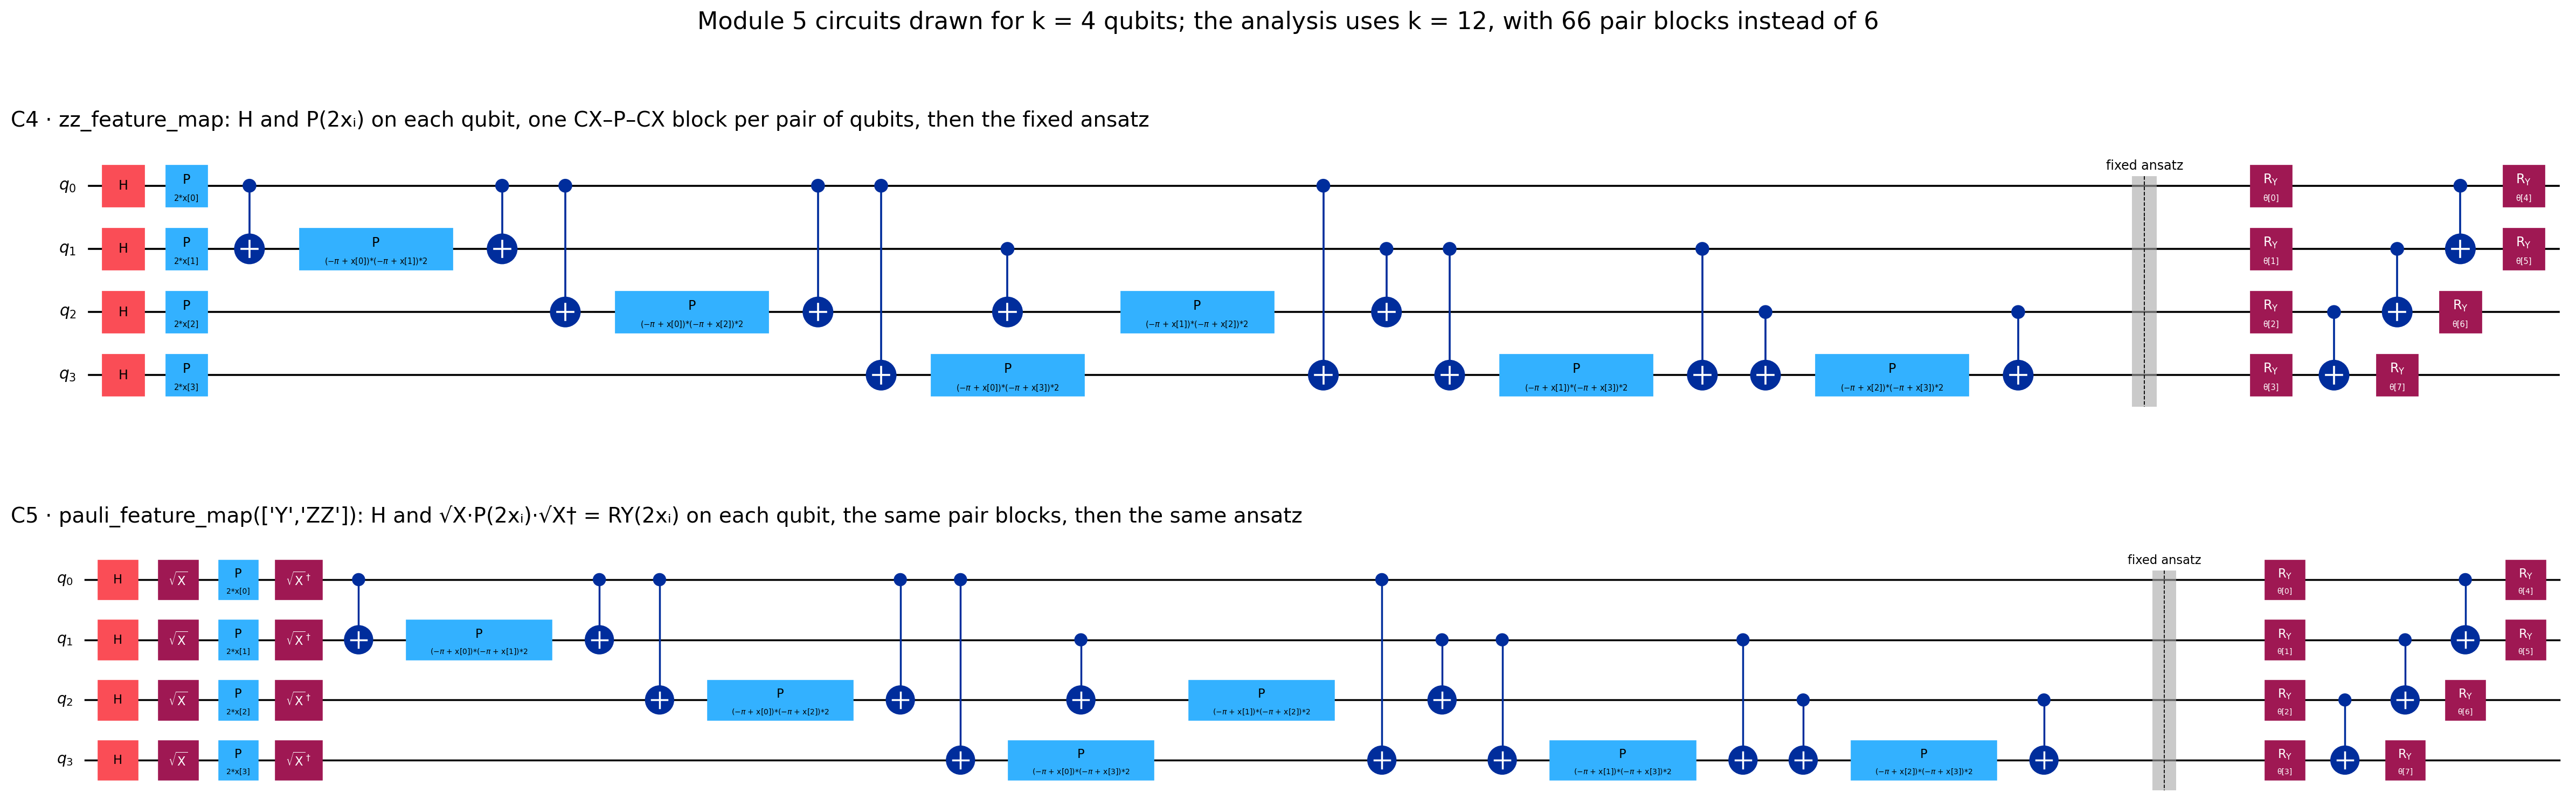
\includegraphics[width=\textwidth]{Figures/M5_circuit_k4.png}
\caption{Circuitos de C4 y C5 dibujados para $k=4$; el análisis usa $k=12$, con 66 bloques de pares en lugar de 6; la barrera separa el \textit{feature map} del \textit{ansatz} fijo.}
\label{fig:circuitos_k4}
\end{figure}

% ---
% Reemplaza líneas 2881–2890 de Docs/Technical_Report.tex (y crea sección propia M6).
% Decisiones que lo respaldan: D-016, D-017, D-027, D-028, D-030, D-032, D-033, D-042,
% H-013, H-032, H-033, H-037, H-038, H-046, H-055.
% ---

\subsection{Módulo 6: Análisis de separabilidad}
\label{sec:modulo6}

El análisis de separabilidad opera sobre dos objetos distintos, y conviene
distinguirlos al interpretar los resultados. Todas las métricas se calculan sobre
la misma submuestra: 200 lesiones del conjunto de entrenamiento por subconjunto,
estratificadas por clase y elegidas con la semilla 42; el conjunto de prueba no interviene.
El tamaño se fijó antes de ver los datos por el coste del protocolo físico: en un equipo cuántico,
cada entrada del kernel es un circuito \textit{compute-uncompute} distinto, de modo que una matriz de
200 lesiones requiere 19\,900 circuitos, frente a cerca de 0.87 y 1.19 millones con todas las masas y
todas las calcificaciones de entrenamiento. En simulación, el cálculo a partir de los vectores de estado
hace viable el conjunto completo; por ello, el experimento X9 (sección~\ref{sec:experimentos_complementarios})
repite las métricas sobre otras 19 submuestras y sobre todo el entrenamiento como análisis de robustez.
Los kernels cuánticos se evalúan de forma exacta a partir de los vectores de estado, y la
significancia de cada métrica que usa las etiquetas se estima con 1\,000 permutaciones de las etiquetas que
conservan el número de lesiones de cada clase.

\textbf{Métricas sobre kernels.} El kernel cuántico de fidelidad
$K_Q(\mathbf{x},\mathbf{x}') = |\langle\phi(\mathbf{x})|\phi(\mathbf{x}')\rangle|^2$ se
evalúa de forma exacta sobre el \textit{feature map} exclusivamente, sin \textit{ansatz}.
Se calculan tres cantidades:
\begin{itemize}
  \item El \textit{kernel-target alignment} centrado \cite{Cortes2012}, con la versión sin
        centrar \cite{cristianini2002kernel} como complemento. Dado que para un kernel cercano a la
        identidad ambas valen aproximadamente $1/\sqrt{N}$ con independencia de las
        etiquetas, se compara el exceso sobre la media de una prueba de permutación.
  \item La dimensión efectiva $d$ del espacio que generan las lesiones \cite{huang2021power}
        (ecuación~\eqref{eq:dim_efectiva}, sección~\ref{sec:metricas}), que cuantifica en cuántas
        direcciones independientes se reparten las lesiones dentro del espacio del kernel: va de
        1, si todas se parecen, a $N$, si cada lesión es ortogonal a las demás, calculada a partir
        de los valores propios ordenados de la matriz del kernel normalizada.
  \item La \textit{geometric difference} regularizada $g_{\mathrm{gen}}$ \cite{huang2021power}
        (ecuaciones~\eqref{eq:g_gen} y~\eqref{eq:g_tra}, sección~\ref{sec:metricas}), sujeta a que
        el error de entrenamiento $g_{\mathrm{tra}}$ sea menor que 0.045.
\end{itemize}

El kernel clásico de referencia $K_C$ es el RBF con el ancho de banda $\gamma$ fijado por la
heurística de la mediana, el mismo de C3. Siguiendo el protocolo de Huang et al. \cite{huang2021power},
se reporta el mínimo sobre una batería de kernels clásicos (un kernel lineal sobre los datos
centrados y nueve kernels gaussianos con $\gamma = m/(n\operatorname{Var}[\mathbf{x}])$, para
$m\in\{0.25,0.5,1,2,4,8,16,32,64\}$) y valores de regularización
$\lambda\in\{10^{-5},10^{-4},10^{-3},10^{-2},0.025,0.05,0.1\}$, con $\operatorname{Tr}(K) = N$. Como
sensibilidad se añaden tres gaussianos más estrechos, $m\in\{128,256,512\}$;
para cada kernel se toma el mayor $\lambda$ admisible que satisface la cota sobre $g_{\mathrm{tra}}$.
Sin regularización, la cantidad mide sobre todo el condicionamiento de $K_C$ y no la codificación.

Como análisis de sensibilidad, los kernels cuánticos se recalculan con los ángulos escalados,
$\mathbf{x}\to c\,\mathbf{x}$, para $c \in \{1, 0.5, 0.2, 0.1, 0.05, 0.02\}$. Así se mide cómo cambia la
geometría cuando las rotaciones son menores.

\textbf{Métricas sobre los \textit{embeddings}.} El índice de Davies-Bouldin, la razón de
Fisher multivariante (ecuación~\eqref{eq:fisher_multivariate}) y el alineamiento del kernel lineal se
calculan sobre los vectores de las cinco condiciones, que son los que recibe el
clasificador; la visualización \textit{t-SNE} (perplejidad 30, inicialización por PCA,
semilla 42) se usa solo como apoyo visual. Las tres métricas son invariantes ante la
rotación de C2, que actúa así como control nulo.

Ambas familias de métricas no son equivalentes: el kernel de fidelidad compara estados
completos, incluida su información de fase, mientras que los valores esperados en la
base $Z$ solo ven la parte de esa información que el \textit{ansatz} convierte en probabilidades.
Por eso las dos familias pueden ordenar las condiciones de forma distinta.

% ---
% Reemplaza líneas 2844–2869 de Docs/Technical_Report.tex.
% Decisiones que lo respaldan: D-014, D-018, D-026, D-030, D-036, D-037,
% H-011, H-035, H-051, H-054.
% ---

\subsection{Módulo 7: Clasificación}
\label{sec:modulo7}

El módulo de clasificación entrena el mismo perceptrón multicapa en PyTorch sobre la
representación de cada condición: una capa de entrada de dimensión 12, capas ocultas de 32 y 16
neuronas con activación ReLU, y una salida sigmoide que da la probabilidad de malignidad. La pérdida
es la entropía cruzada binaria ponderada (ecuación~\eqref{eq:weighted_bce}), con los pesos de la
ecuación~\eqref{eq:class_weights}, optimizada con Adam (tasa $10^{-3}$, decaimiento de pesos
$10^{-4}$, lotes de 128). Las entradas se estandarizan con la media y la desviación del
entrenamiento de cada ajuste: las representaciones difieren en escala en más de un orden de magnitud (en masas, desviación típica media por dimensión de 0.90 en C1 frente a 0.056 en C4), y
sin estandarizar el optimizador favorecería a las de escala grande por una razón ajena a su
información. El entrenamiento se detiene cuando la pérdida, medida sobre el 15\,\% de los pacientes
del entrenamiento, deja de mejorar durante 40 épocas, y se conservan los mejores pesos. Los
hiperparámetros se fijaron antes de ver los resultados y son idénticos en las cinco condiciones, con
la misma semilla.

Cada condición se evalúa con validación cruzada de cinco \textit{folds}, los fijados en M4, y con un
único ajuste sobre todo el entrenamiento que se evalúa una sola vez en el conjunto de prueba oficial.
La incertidumbre del conjunto de prueba se estima con 2\,000 remuestreos \textit{bootstrap} por
paciente, pareados entre condiciones. El selector y el escalador de M4 se ajustan una sola vez con todo
el entrenamiento, no dentro de cada \textit{fold}, así que la validación cruzada es algo optimista;
volver a seleccionar dentro de cada \textit{fold} cambia el AUC en 0.006 o menos.

Los parámetros $\boldsymbol\theta$ del circuito no se entrenan. La razón principal es de validez
interna: C2 y C3 son transformaciones que no ven las etiquetas, y si C4 y C5 ajustaran
$\boldsymbol\theta$ contra ellas, cualquier ventaja podría deberse al ajuste supervisado y no a la
codificación. Además, la pregunta de investigación se refiere a la codificación $\phi$ y no a un
procedimiento de optimización. Una tercera razón es el costo: con el método de
\textit{parameter-shift}, el que puede usarse en un computador cuántico, entrenar $\boldsymbol\theta$, medido en el simulador,
costaría unas 205 horas por \textit{feature map}. En el simulador existe un atajo: retropropagar a
través del vector de estado da el mismo gradiente unas 3\,600 veces más rápido. Pero ese atajo no
existe en el hardware, porque exige conocer todas las amplitudes del estado. La sensibilidad de la
conclusión a la semilla, la red, el escalado, la parada temprana, \texttt{reps} y $k$ se reporta en
la sección de resultados.

% ---
% Reemplaza líneas 2872–2921 de Docs/Technical_Report.tex.
% Decisiones que lo respaldan: D-030, D-039, D-040, H-049, H-052.
% ---

\subsection{Módulo 8: Evaluación comparativa}
\label{sec:modulo8}

El módulo de evaluación compara las cinco condiciones a partir de los resultados de M6 y M7, sin
volver a usar el conjunto de prueba.

\textbf{Métricas de clasificación.} Se reportan AUC-ROC, F1, \textit{accuracy}, \textit{precision}
y \textit{recall} en el conjunto de prueba, por condición y por tipo de hallazgo. El AUC-ROC es la
métrica principal, porque no depende de un umbral de decisión y es robusta al desbalance de clases;
las demás usan el umbral 0.5.

\textbf{Correlación entre separabilidad y clasificación.} Se calcula el coeficiente de Spearman
$\rho_s$ entre el ordenamiento de las cinco condiciones según cada métrica de separabilidad y su
ordenamiento según el AUC-ROC. Con cinco condiciones solo hay $5! = 120$ órdenes posibles, y sin
empates solo el acuerdo perfecto alcanza $p < 0.05$. Además, C1 y C2 empatan en toda métrica de
separabilidad por construcción. Por eso $\rho_s$ se reporta de forma descriptiva, por subconjunto y
con su distribución exacta, y se calcula como la correlación de Pearson entre rangos promedio, que
admite empates (ecuación~\eqref{eq:spearman}).

\textbf{Masas frente a calcificaciones.} Para interpretar la diferencia de dificultad entre
subconjuntos, se ajusta una regresión logística sobre los descriptores que el CBIS-DDSM registra
para cada lesión: forma y márgenes en masas, tipo y distribución en calcificaciones. Es una
referencia, no un competidor: esos descriptores los escribió un radiólogo viendo la imagen.

\textbf{Restricciones del simulador (OE-6).} Se miden el tiempo por muestra y el número máximo de
qubits viable en el equipo de trabajo, y el costo del entrenamiento por \textit{parameter-shift}. El
efecto del número de \textit{shots} se mide de dos formas. En el \textit{embedding}, se simulan
mediciones con $n$ disparos a partir de las probabilidades exactas, con $n$ de 64 a 65\,536, y se
reentrena el clasificador. En el kernel, se calcula de forma analítica el número de disparos que
exigiría estimar cada valor en hardware.

% ---
% Experimentos complementarios (X1--X8) y estudios de caracterización del simulador (B1--B3).
% Sección metodológica previa al reporte de resultados.
% Entradas que lo respaldan: H-018, H-019, H-035, H-036, H-041, H-044, H-045, H-046, H-047, H-048, H-051, H-052, H-053, H-054, D-035, D-038.
% ---

\subsection{Experimentos complementarios}
\label{sec:experimentos_complementarios}

Con el propósito de evaluar la solidez de las conclusiones obtenidas en el protocolo principal frente a hipótesis
alternativas o variantes metodológicas que un lector u evaluador razonable plantearía, se diseñó una batería de ocho
experimentos complementarios (denominados X1 a X8). Estos experimentos no alteran el diseño experimental básico ni
los puntos de decisión congelados para el pipeline principal ($k = 12$, $reps = 1$, Arquitectura~B con vector de
parámetros $\boldsymbol\theta$ fijo con semilla 42 y particiones independientes por paciente), sino que someten a
prueba la sensibilidad de los hallazgos ante variaciones controladas en la selección de características, la dimensionalidad
del registro cuántico, la arquitectura de clasificación, la optimización variacional y el protocolo de evaluación.
La Tabla~\ref{tab:resumen_experimentos_complementarios} resume las características de diseño de cada experimento, y
los párrafos siguientes detallan su formulación metodológica. Los resultados cuantitativos derivados de estas pruebas se
reportan en el Capítulo~\ref{sec:resultados}.

% fuente: H-035, H-036, H-041, H-044, H-045, H-046, H-047, H-048, H-053, H-054, D-035, D-038
\begin{table}[htbp]
\centering
\small
\caption{Resumen de diseño de los experimentos complementarios X1 a X8.}
\label{tab:resumen_experimentos_complementarios}
\begin{adjustbox}{max width=\linewidth}
\begin{tabular}{p{0.06\linewidth} p{0.22\linewidth} p{0.28\linewidth} p{0.22\linewidth} p{0.18\linewidth} p{0.14\linewidth}}
\toprule
\textbf{Exp.} & \textbf{Nombre / Archivo} & \textbf{Pregunta metodológica} & \textbf{Variación vs. Fijo} & \textbf{Control} & \textbf{Uso de prueba} \\
\midrule
X1 & \texttt{X1\_Selection\_}\allowbreak\texttt{Information\_Loss} & ¿Cuánta información se pierde al reducir de 67 a 12 variables? & Varía subconjunto de variables; fijos modelos clásicos. & 67 variables y PCA con 12 componentes. & No (solo entrenamiento). \\
X2 & \texttt{X2\_Kernel\_}\allowbreak\texttt{Class\_Structure} & ¿Conservan los kernels cuánticos similitud intra-clase? & Varía escala $c$; fijos kernels de C4 y C5. & Kernel RBF clásico y permutación. & No (submuestra de entrenamiento). \\
X3 & \texttt{X3\_Fewer\_Qubits\_}\allowbreak\texttt{k8} & ¿Persiste la conclusión con un registro de $k = 8$ qubits? & Varía $k \in \{8, 12\}$; fijo protocolo de métricas. & Condiciones clásicas con 8 variables. & No en separabilidad; sensibilidad en M7. \\
X4 & \texttt{X4\_QSVM\_and\_}\allowbreak\texttt{67\_Features} & ¿Se pierde información en la codificación o en la lectura? & Varía clasificador (QSVM vs MLP) y variables ($k=12$ vs 67). & SVM clásico RBF y MLP de M7. & Sí (una vez por configuración). \\
X5 & \texttt{X5\_Pipeline\_}\allowbreak\texttt{Audit} & ¿Existe algún fallo de implementación o fuga de datos? & Varía implementación de componentes; fijos datos. & Implementaciones alternativas y código Qiskit. & Sí (solo verificación de partición). \\
X6 & \texttt{X6\_Searching\_}\allowbreak\texttt{for\_Advantage} & ¿Supera algún kernel cuántico al clásico en etiquetas reales? & Búsqueda anidada sobre familias cuánticas y clásicas. & Mejores modelos clásicos y etiquetas de Huang. & Sí (una vez por mejor modelo). \\
X7 & \texttt{X7\_Theta\_}\allowbreak\texttt{Draws} & ¿Introduce sesgo el sorteo único de $\boldsymbol\theta$? & Varía semilla de $\boldsymbol\theta$ (10 sorteos); fijo MLP. & Variabilidad de MLP y condiciones clásicas. & No (solo validación cruzada). \\
X8 & \texttt{X8\_Trained\_}\allowbreak\texttt{Theta} & ¿Mejora la representación al entrenar $\boldsymbol\theta$? & Varía optimización de $\boldsymbol\theta$ (entrenado vs fijo); fijo MLP. & Modelo con $\boldsymbol\theta$ fijo de M7 y C1 crudo. & Sí (una vez por subconjunto y mapa). \\
\bottomrule
\end{tabular}
\end{adjustbox}
\end{table}

% fuente: H-035
\textbf{Experimento X1: Pérdida de información en la selección de características.} Desarrollado en
\texttt{Code/}\allowbreak\texttt{experiments/}\allowbreak\texttt{X1\_Selection\_Information\_Loss.ipynb}, este análisis responde a la
interrogante de cuánta información diagnóstica y varianza global se descarta al reducir el conjunto radiómico de 67 a 12
variables en M4. En su diseño se compara la capacidad predictiva y la varianza retenida evaluando distintos subconjuntos
de características: las 67 originales, las 12 seleccionadas por el protocolo estándar, 12 variables reajustadas dentro de
cada pliegue de validación cruzada, las 12 mejores según la prueba F univariante sin filtro de redundancia, y conjuntos de
12 variables elegidas al azar. Como control se emplean modelos clásicos de regresión logística y bosques aleatorios ajustados
exclusivamente dentro de los pliegues de validación cruzada sobre el conjunto de entrenamiento, junto con una descomposición
PCA de 12 componentes como cota lineal de retención de varianza. Este experimento no utiliza el conjunto de prueba oficial.
Los resultados se analizan en la Sección~\ref{sec:datos_caracteristicas_seleccion}.

% fuente: H-036
\textbf{Experimento X2: Estructura de clase en matrices de kernel.} Implementado en
\texttt{Code/}\allowbreak\texttt{experiments/}\allowbreak\texttt{X2\_Kernel\_Class\_Structure.ipynb}, evalúa si dos lesiones de la misma
clase diagnóstica (benigna--benigna o maligna--maligna) exhiben mayor similitud de Hilbert que dos lesiones de clases opuestas,
y en qué medida dicha diferenciación depende del factor de contracción angular $c$. El diseño analiza la distribución de
similitudes por pares de lesiones sobre la submuestra estratificada de 200 casos de entrenamiento, calculando el área
bajo la curva ROC de pares frente a un barrido del parámetro de escala angular. Como control de referencia se utiliza el kernel
gaussiano RBF clásico con ancho de banda calibrado por la heurística de la mediana, contrastando la significancia estadística
frente a una prueba de permutación de 1\,000 iteraciones con etiquetas barajadas. El experimento prescinde del conjunto de prueba.
Sus resultados se presentan en la Sección~\ref{sec:separabilidad_representaciones}.

% fuente: H-041, D-035
\textbf{Experimento X3: Evaluación con registro reducido ($k = 8$ qubits).} Desarrollado en
\texttt{Code/}\allowbreak\texttt{experiments/}\allowbreak\texttt{X3\_Fewer\_Qubits\_k8.ipynb}, examina si la ausencia de ventaja cuántica
en separabilidad observada en M6 es atribuible a la concentración exponencial del espacio de Hilbert a $k = 12$ qubits. El diseño
mantiene idénticos los protocolos de evaluación de KTA, dimensión efectiva, diferencia geométrica regularizada $g$ y razón de Fisher,
variando la dimensión del registro cuántico a $k = 8$ qubits (lo que reduce los acoplamientos $ZZ$ de 66 a 28 bloques y los parámetros
del circuito variacional de 24 a 16). Se toman de forma determinista las 8 primeras características del ordenamiento de M4. Como control,
se evalúan las condiciones clásicas C1, C2 y C3 sobre las mismas 8 características de entrada. En la fase de separabilidad este
experimento no accede al conjunto de prueba oficial, mientras que su traslación a clasificación se evalúa en el análisis de sensibilidad
del Módulo~7. Los resultados se detallan en la Sección~\ref{sec:separabilidad_representaciones}.

% fuente: H-044, H-045, D-038
\textbf{Experimento X4: Máquinas de soporte vectorial cuánticas y codificación de 67 variables.} Ejecutado en
\texttt{Code/}\allowbreak\texttt{experiments/}\allowbreak\texttt{X4\_QSVM\_and\_67\_Features.ipynb}, busca determinar si la pérdida de
desempeño observada en M7 reside intrínsecamente en la codificación cuántica en el espacio de Hilbert o en la etapa de lectura
mediante expectativas locales $\langle Z_i \rangle$ bajo la Arquitectura~B. Para ello, se implementa una máquina de vectores de
soporte con kernel cuántico (QSVM) evaluada directamente sobre las matrices completas de fidelidad de C4 y C5. Asimismo, se evalúa si
la disponibilidad de las 67 características radiómicas completas permite formular kernels cuánticos con ventaja frente al límite
clásico, analizando codificaciones en amplitud sobre 7 qubits y codificaciones angulares en producto tensorial sobre 67 qubits. Se
contrasta directamente contra modelos SVM clásicos lineales y RBF, así como contra el clasificador MLP entrenado sobre las expectativas
de M7. Los modelos se optimizan mediante validación cruzada y se evalúan una única vez sobre el conjunto de prueba oficial.
Los resultados se reportan en la Sección~\ref{sec:qsvm_ventaja}.

% fuente: H-046
\textbf{Experimento X5: Auditoría independiente del pipeline experimental.} Documentado en
\texttt{Code/}\allowbreak\texttt{experiments/}\allowbreak\texttt{X5\_Pipeline\_Audit.ipynb}, responde a la necesidad metodológica de
descartar que la ausencia de ventaja cuántica provenga de anomalías de software, fugas de datos (*data leakage*) entre entrenamiento
y prueba, asimetrías de preprocesamiento o discrepancias numéricas en el cómputo de fidelidades. La auditoría consta de 25 pruebas
programadas independientes que reconstruyen particiones y diagnósticos directamente desde las fuentes maestras de metadatos,
contrastan la simulación de kernels mediante circuitos físicos frente a la formulación por vectores de estado, y verifican la
equivalencia de las implementaciones clasificatorias frente a bibliotecas estándar de la comunidad. El conjunto de prueba se
utiliza exclusivamente para verificar la integridad y aislamiento de las particiones, sin entrenamiento ni ajuste de parámetros.
Su análisis se discute en la Sección~\ref{sec:qsvm_ventaja}.

% fuente: H-047, H-048
\textbf{Experimento X6: Búsqueda exhaustiva de ventaja cuántica y contraste con etiquetas sintéticas.} Desarrollado en
\texttt{Code/}\allowbreak\texttt{experiments/}\allowbreak\texttt{X6\_Searching\_for\_Advantage.ipynb}, plantea una búsqueda anidada y
simétrica de configuraciones óptimas en ambos paradigmas. En el lado cuántico se exploran mapas $ZZ$ con entrelazamiento lineal y
completo, repeticiones $reps \in \{1, 2\}$, factores de escala angular y kernels proyectados; en el lado clásico se evalúan familias
gaussianas, lineales y polinomiales. Para discernir si la ausencia de ventaja obedece al protocolo experimental o a la relación
geométrica intrínseca de las etiquetas patológicas reales, se incorpora una prueba de contraste con etiquetas sintéticas generadas
según la metodología de Huang et al., alineadas por construcción con la métrica del kernel cuántico. La selección de modelos se efectúa
mediante validación cruzada anidada y la evaluación en el conjunto de prueba se restringe a una sola ejecución por contendiente global.
Los resultados se exponen en la Sección~\ref{sec:qsvm_ventaja}.

% fuente: H-053
\textbf{Experimento X7: Sensibilidad al vector de parámetros variacionales $\boldsymbol\theta$.} Implementado en
\texttt{Code/}\allowbreak\texttt{experiments/}\allowbreak\texttt{X7\_Theta\_Draws.ipynb}, evalúa si la fijación de $\boldsymbol\theta$
mediante un único sorteo aleatorio (semilla 42) en la Arquitectura~B introdujo un sesgo desfavorable para las representaciones
cuánticas C4 y C5. El diseño analiza diez sorteos pseudoaleatorios independientes del vector $\boldsymbol\theta$ (semillas 42 a 51),
manteniendo fijos la semilla del clasificador MLP, la arquitectura de red y los pliegues de validación cruzada de M7. Como control
se compara la variación inducida por el parámetro $\boldsymbol\theta$ frente a la variabilidad por semilla de inicialización del
MLP clásico y frente a los desempeños obtenidos por C1 y C3. Este análisis opera de forma estricta sobre el conjunto de entrenamiento
en validación cruzada sin tocar el conjunto de prueba. Sus resultados se reportan en la Sección~\ref{sec:rendimiento_clasificacion}.

% fuente: H-054
\textbf{Experimento X8: Optimización variacional conjunta de $\boldsymbol\theta$.} Realizado en
\texttt{Code/}\allowbreak\texttt{experiments/}\allowbreak\texttt{X8\_Trained\_Theta.ipynb}, examina si el entrenamiento supervisado
de los parámetros $\boldsymbol\theta$ en forma simultánea con los pesos del clasificador MLP permite cerrar la brecha de rendimiento
observada frente a las condiciones clásicas. En este esquema, el vector de expectativas alimenta una capa diferencial que actualiza
$\boldsymbol\theta$ mediante retropropagación sobre el vector de estado simulado en PyTorch con una tasa de aprendizaje dedicada. Se
analiza la sensibilidad ante la inicialización de $\boldsymbol\theta$ y se compara el modelo resultante frente a la condición fija
de M7, frente a la condición clásica C1 y frente al clasificador QSVM de X4. El conjunto de prueba oficial se consulta exactamente
una vez por modelo optimizado. Los resultados se analizan en las Secciones~\ref{sec:rendimiento_clasificacion} y~\ref{sec:restricciones_simulador}.

% fuente: H-018, H-019, H-051, H-052
\textbf{Estudios de caracterización del simulador cuántico (B1--B3).} De forma complementaria a los experimentos sobre datos radiómicos,
se llevaron a cabo tres estudios sistemáticos en \texttt{Code/benchmark/} para cuantificar las restricciones operacionales de la simulación
clásica de circuitos cuánticos en el contexto del proyecto. El estudio B1 (\texttt{B1\_Quantum\_Benchmark.ipynb}) midió la complejidad
estructural de los circuitos (profundidad, número de compuertas CX y conteo total de compuertas en función de $k$ y $reps$) y proyectó
el coste computacional del entrenamiento conjunto bajo la Arquitectura~A frente al esquema de precomputación de la Arquitectura~B.
No obstante, la sección de sensibilidad al número de disparos (*shots*) de B1 quedó formalmente invalidada debido a que la referencia
analítica empleada incorporaba ruido gaussiano no nulo inyectado por omisión de precisión cero en el estimador de alto nivel.
El estudio B2 (\texttt{B2\_Design\_Verifications.ipynb}) integró las comprobaciones empíricas que respaldaron las decisiones de diseño
metodológico: número de qubits y profundidad, arquitectura del \textit{embedding}, condiciones experimentales, cálculo de la \textit{geometric difference} y validación cruzada. Finalmente, el estudio B3 (\texttt{B3\_Sampling\_and\_Concentration.ipynb}) sustituyó y rectificó la caracterización
de disparos de B1 mediante un esquema de muestreo real con el estimador por muestreo de cadenas de bits de Aer, verificando el escalamiento
estadístico de error teórico $1/\sqrt{n}$ sin suelo de dispersión espuria hasta $2^{20}$ disparos, además de cuantificar la concentración
asintótica del vector de expectativas en función de la dimensionalidad $k$ y la profundidad del circuito. Sus hallazgos se integran en
las Secciones~\ref{sec:restricciones_simulador} y~\ref{sec:lecciones_implementacion}.

\newpage

% ===== Capítulo: 6_Resultados
\setcounter{section}{5}
% ---
% Reemplaza líneas 3452–3461 de Docs/Technical_Report.tex.
% Decisiones que lo respaldan: D-028, D-030.
% ---

\newpage
\section{Resultados}
\addcontentsline{toc}{section}{Resultados}
\label{sec:resultados}

% fuente: D-028
La presentación de los resultados experimentales sigue el orden establecido por los
módulos del sistema. A lo largo de todo el análisis, los subconjuntos de masas y de
calcificaciones se reportan de forma independiente debido a sus diferencias radiológicas
y metodológicas. El conjunto de prueba oficial se reserva exclusivamente para la evaluación
final del modelo de clasificación, garantizando que ninguna etapa previa acceda a dichos casos.
Por su parte, las métricas de separabilidad geométrica se evalúan sobre una submuestra
estratificada de 200 lesiones del conjunto de entrenamiento por subconjunto.

% ---
% Reemplaza parte de la sección de resultados en Docs/Technical_Report.tex.
% Entradas que lo respaldan: H-005, H-020, H-021, H-022, H-023, H-024, H-025, H-026, H-027, H-028, H-030, H-035, D-026.
% ---

\subsection{Datos, características y selección}
\label{sec:datos_caracteristicas_seleccion}

% fuente: H-020; 2_preprocesamiento_qa.csv, 2_discordantes_sensibilidad.csv
En la auditoría del preprocesamiento sobre los 3\,568 registros del conjunto de datos,
se identificaron exactamente 80 máscaras cuyas dimensiones espaciales diferían de las de su
mamografía correspondiente. Estas correspondieron a dos categorías: 78 casos de masas
escalados de forma uniforme por un factor cercano a 0.870 (0.8700 a 0.8704 tanto en filas como en columnas),
y 2 casos de calcificaciones con un ligero desplazamiento espacial. Al contrastar las anotaciones
con los recortes oficiales proporcionados en el conjunto de datos, la regla geométrica de coincidencia
se verificó al píxel en 3\,206 de 3\,213 casos evaluables (99.8\,\%). Se detectaron únicamente 7 casos
discordantes en masas (4 en entrenamiento y 3 en prueba), en los cuales la máscara y el recorte describen
extensiones disímiles de la lesión. La exclusión de los 3 casos de prueba modifica el área bajo la curva
ROC (AUC) en el conjunto de prueba de masas entre $+0.001$ y $+0.004$ a través de las cinco condiciones
evaluadas, y ninguno de estos casos forma parte de la submuestra de 200 casos de separabilidad.

% fuente: H-021; 2_preprocesamiento_qa.csv
Respecto a la topología de las máscaras binarias, 1\,464 de las 1\,696 lesiones de masas
(86.3\,\%) presentaron islas desconectadas, frente a 0 de las 1\,872 lesiones de calcificaciones.
En todos los casos de masas, la componente conexa de mayor tamaño retuvo al menos el 99.55\,\% del área total.
La supresión de componentes menores descartó una mediana de 5 píxeles por máscara (con un valor máximo
de 110 píxeles, equivalente al 0.45\,\% del área de la lesión). La distancia del píxel descartado más lejano
al borde de la componente mayor presentó una mediana de 3.6 píxeles, un percentil 99 de 9.2 píxeles
y un máximo de 14 píxeles, lo que resulta consistente con la hipótesis de que las islas corresponden a artefactos periféricos inmediatos al contorno.

% fuente: H-023, H-024; 3_tamano_efecto.csv
En la etapa de extracción de características radiómicas sobre el conjunto de entrenamiento
(637 lesiones malignas y 681 benignas en masas; 544 malignas y 1\,002 benignas en calcificaciones),
la evaluación univariante mediante la distancia estandarizada de Cohen ($|d|$) mostró que, en las
características extraídas para este conjunto de entrenamiento, las calcificaciones alcanzan tamaños de efecto
individual superiores a los de las masas. En masas, la característica
con mayor tamaño de efecto fue \texttt{firstorder\_Maximum} con $|d| = 0.50$ (con un rango de 0.40 a 0.50
en las doce primeras), seguida de descriptores morfológicos como
\texttt{shape2D}\allowbreak\texttt{\_MinorAxisLength} ($|d| = 0.45$),
\texttt{shape2D}\allowbreak\texttt{\_MaximumDiameter} ($|d| = 0.44$)
y \texttt{shape2D}\allowbreak\texttt{\_MajorAxisLength} ($|d| = 0.43$). Por su parte, en calcificaciones
la característica más discriminativa fue \texttt{shape2D}\allowbreak\texttt{\_MinorAxisLength} con $|d| = 0.82$
(con un rango de 0.64 a 0.82 en las doce primeras), seguida de \texttt{shape2D}\allowbreak\texttt{\_Perimeter} ($|d| = 0.71$).

% fuente: H-023, H-024; 3_tamano_efecto.csv
En el subconjunto de masas se observó que los primeros puestos del ordenamiento corresponden a
características de primer orden calculadas sobre intensidades sin calibrar (\texttt{Maximum}, \texttt{90Percentile},
\texttt{Energy}, \texttt{Median} y \texttt{Mean}). Dado que la base de datos combina digitalizadores sin consignar
el fabricante en los metadatos correspondientes, no es posible descartar que parte de dicha señal provenga de
diferencias en la adquisición física de la imagen. Adicionalmente, el ordenamiento univariante directo en masas
seleccionó 7 características de primer orden y 5 morfológicas sin incluir ninguna variable de textura
(0 de matrices de coocurrencia GLCM y 0 de matrices de longitud de rachas GLRLM), exhibiendo una correlación
media intercaracterística de $|r| = 0.61$ con 8 pares por encima de $|r| > 0.95$, además de duplicados exactos
en dos dimensiones tales como \texttt{Energy} y \texttt{TotalEnergy}, o \texttt{MeshSurface} y \texttt{PixelSurface} ($r = 1.0000$).
En calcificaciones, el conjunto preliminar incluyó 1 característica de primer orden, 2 morfológicas, 4 de GLCM
y 5 de GLRLM, con una correlación media de $|r| = 0.58$ y 5 pares con $|r| > 0.95$.

% fuente: H-025; 3_efecto_clahe.csv
La aplicación de ecualización adaptativa de histograma con limitación de contraste (CLAHE)
reordenó las lesiones con una correlación de Spearman cercana a 0.84 respecto a las intensidades crudas,
pero no aportó ganancia discriminativa neta. La variación mediana en $|d|$ fue de $-0.002$ en masas
y de $-0.010$ en calcificaciones. Las características de intensidad de primer orden sufrieron una reducción
mediana de $|d|$ de $-0.031$ en masas y de $-0.054$ en calcificaciones, compensada únicamente por incrementos
menores en descriptores de textura (GLRLM $+0.011$ en masas, GLCM $+0.014$ en calcificaciones), sin mejorar
el poder de separación de las características dominantes (figuras~\ref{fig:m3_effect_sizes} y~\ref{fig:m3_clahe_effect}).

\begin{figure}[htbp]
\centering
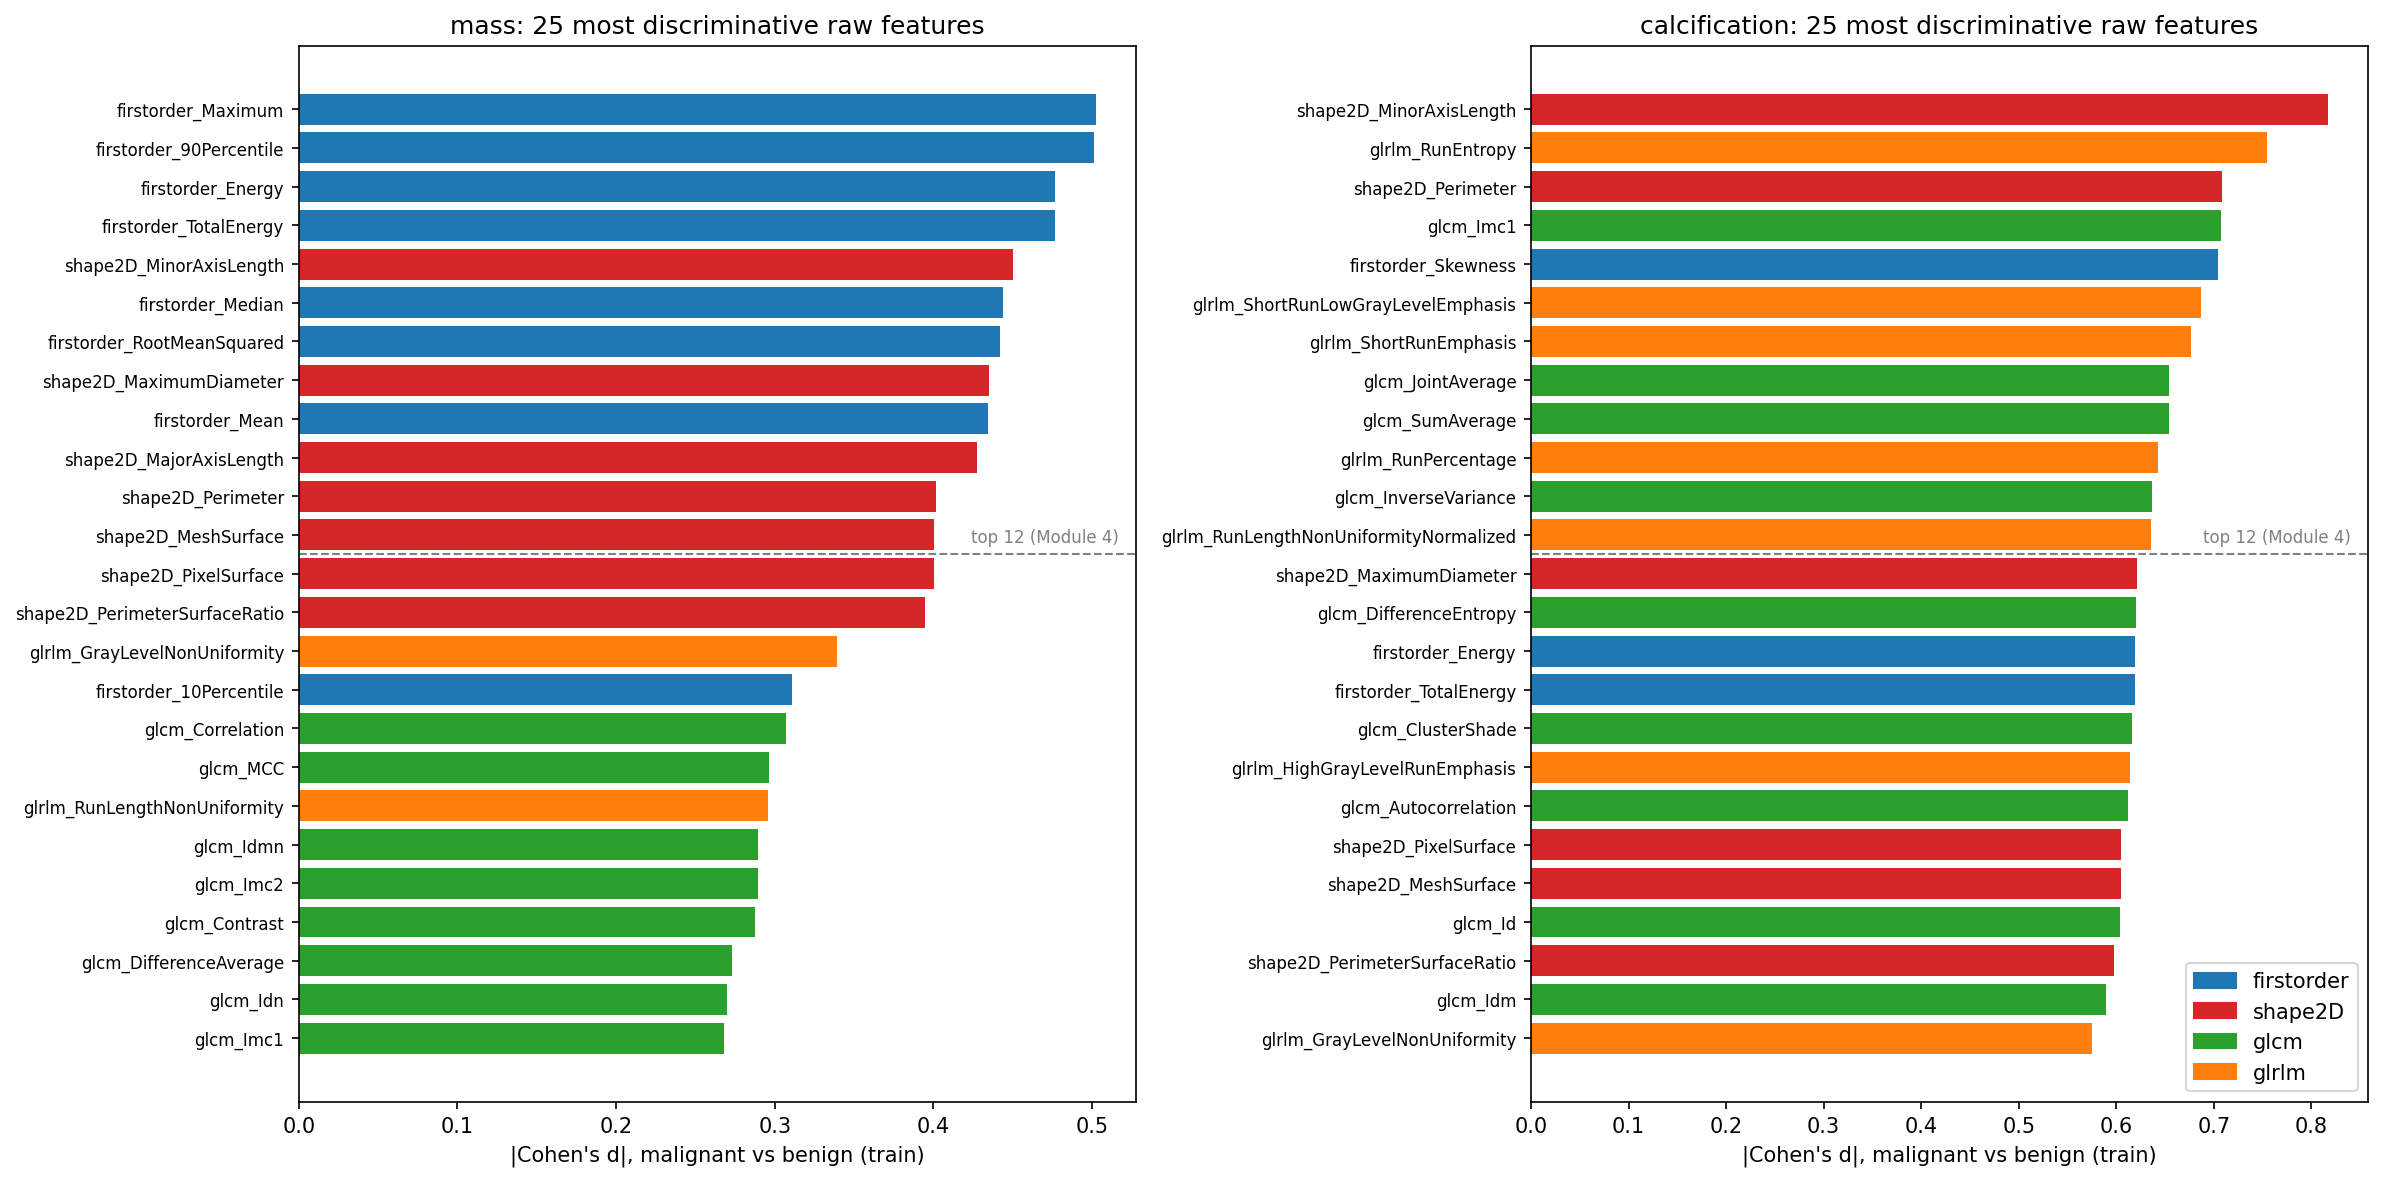
\includegraphics[width=\textwidth]{Figures/M3_effect_sizes.png}
% fuente: H-023; 3_tamano_efecto.csv
\caption{Tamaños de efecto de Cohen ($|d|$) para las características radiómicas evaluadas en el conjunto de entrenamiento de masas y calcificaciones.}
\label{fig:m3_effect_sizes}
\end{figure}

\begin{figure}[htbp]
\centering
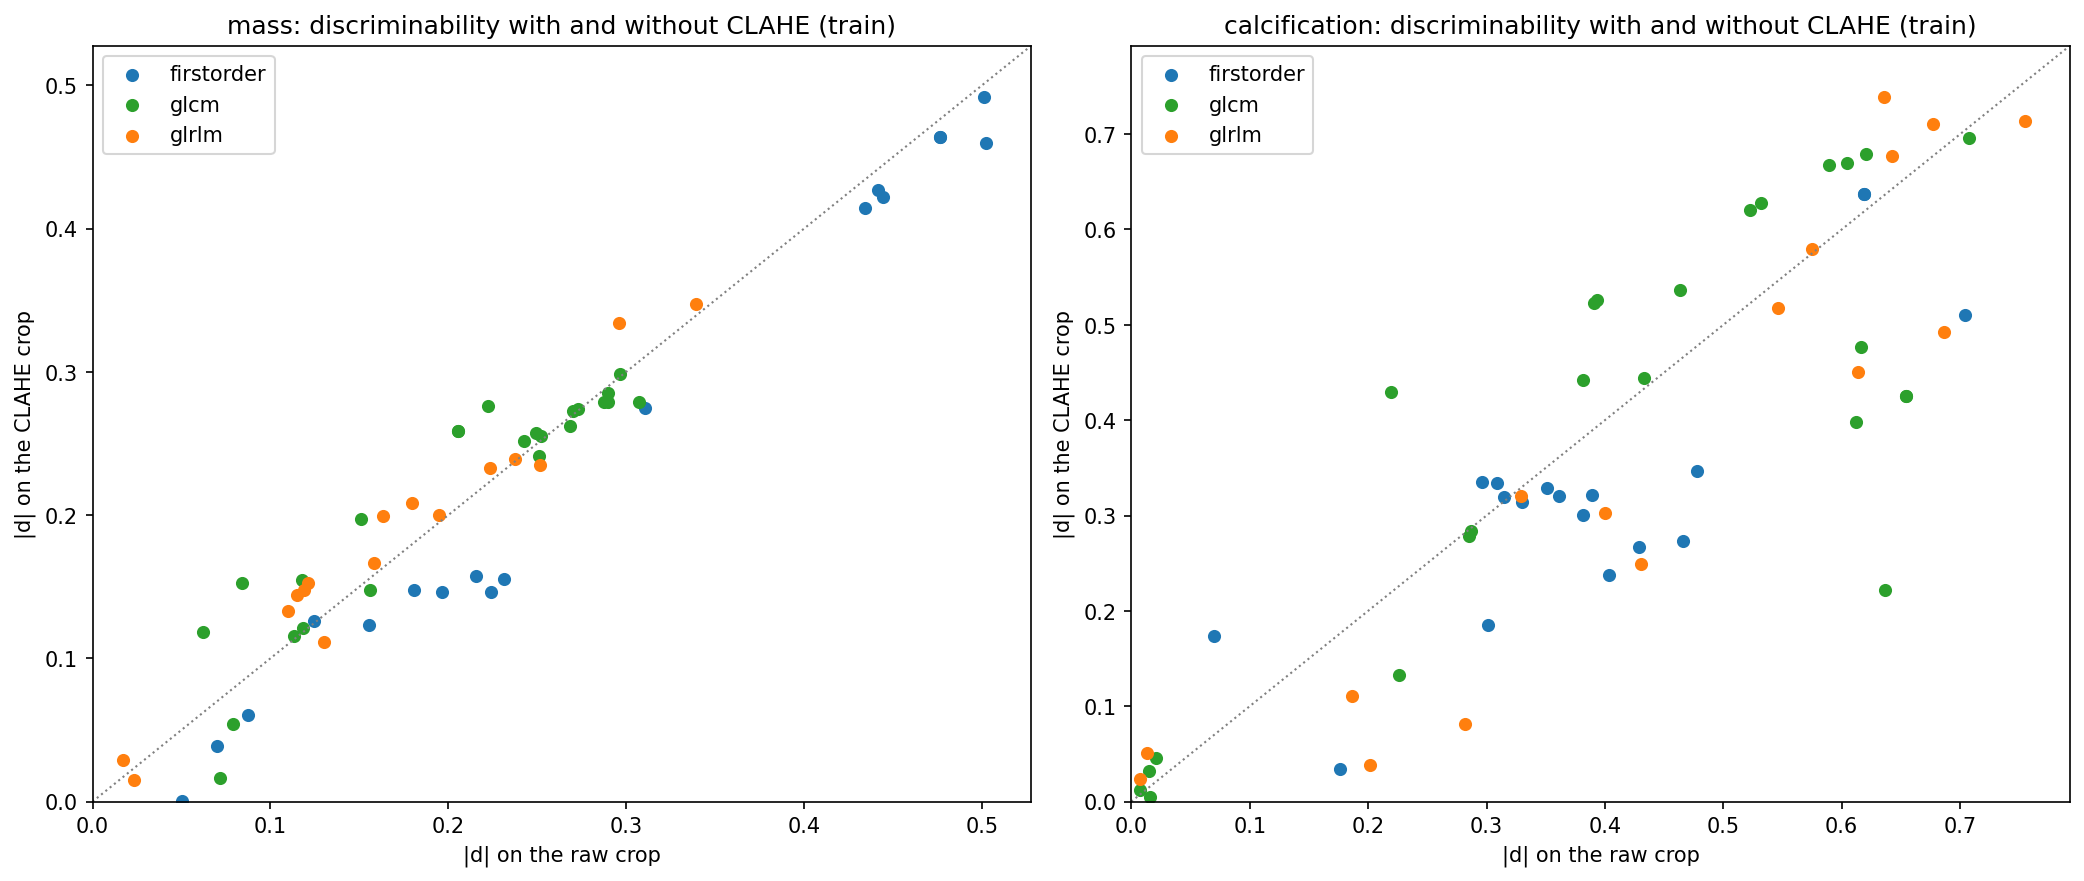
\includegraphics[width=\textwidth]{Figures/M3_clahe_effect.png}
% fuente: H-025; 3_efecto_clahe.csv
\caption{Efecto de la ecualización CLAHE sobre la capacidad discriminativa y el reordenamiento de características radiómicas por familia.}
\label{fig:m3_clahe_effect}
\end{figure}

% fuente: H-026; 4_seleccion.csv, 4_descartadas_redundancia.csv, 4_sensibilidad_umbral.csv
Para la selección final a doce características, la incorporación de la restricción de redundancia
($|r| \le 0.95$) descartó 7 variables redundantes en masas y 8 en calcificaciones, eliminando los duplicados
analíticos. En masas, la composición final se rebalanceó a 4 características de primer orden, 5 morfológicas,
1 de GLCM y 2 de GLRLM, reduciendo la correlación media a $|r| = 0.50$ y el valor máximo a $|r| = 0.94$.
La entrada de descriptores de textura en masas se mantuvo estable ante variaciones del umbral de correlación
entre 0.99 y 0.80. En calcificaciones, el conjunto final reunió 2 características de primer orden, 3 morfológicas,
4 de GLCM y 3 de GLRLM, con una correlación media de $|r| = 0.50$. Las doce variables resultantes se presentan
en la Tabla~\ref{tab:m4_seleccion}.

% fuente: H-026; 4_seleccion.csv
\input{tablas/m4_seleccion}

% fuente: H-028; 4_seleccion.csv
En la etapa de escalado angular, el uso de escalado por valores extremos (\texttt{MinMaxScaler})
hacia el intervalo $[0, \pi]$ comprimía excesivamente las distribuciones de aquellas características con colas
pesadas. En calcificaciones, el rango intercuartílico (IQR) de \texttt{firstorder\_\allowbreak Energy} resultaba
en $0.046$\,rad (con mediana de $0.015$\,rad) y el de \texttt{shape2D\_\allowbreak PixelSurface} en $0.057$\,rad
(mediana de $0.020$\,rad), en contraste con una mediana global de IQR de $0.34$\,rad en masas y $0.40$\,rad en
calcificaciones. La adopción de una transformación por cuantiles hacia una distribución uniforme en $[0, \pi]$
permitió que las doce características en ambos subconjuntos alcanzaran de forma homogénea un IQR de $\pi/2$
($1.569$ a $1.572$\,rad; figura~\ref{fig:m4_selection_angles}).

% fuente: H-027, D-026; 4_semilla_folds.csv, 4_folds.csv
Para la partición en cinco pliegues de validación cruzada, la agrupación por paciente evitó
la fragmentación de estudios pertenecientes a un mismo individuo, la cual afectaba al 59\,\% de los pacientes
en masas y al 74\,\% en calcificaciones bajo particiones estratificadas simples. Al evaluar la partición inicial
con semilla 42, el segundo pliegue de calcificaciones exhibió un 52\,\% de casos malignos frente al 35\,\%
poblacional (desviación de 0.168). La selección mediante búsqueda sistemática entre 200 semillas identificó
la semilla 125 en masas y la semilla 168 en calcificaciones, acotando la desviación máxima de malignidad
a 0.011 en masas y a 0.019 en calcificaciones (proporciones entre 0.33 y 0.37 por pliegue).

% fuente: H-005
En cuanto a la división entre los conjuntos de entrenamiento y prueba, la auditoría de partición confirmó
la ausencia de fuga de pacientes (\textit{data leakage}) dentro de cada subproblema analizado.
En masas se contabilizaron 691 pacientes en entrenamiento y 201 en prueba sin solapamiento alguno (0 pacientes
compartidos); análogamente, en calcificaciones se identificaron 602 pacientes en entrenamiento y 151 en prueba,
igualmente con 0 solapes. A nivel global, considerando ambos hallazgos de forma conjunta, se registraron 1\,248
pacientes en entrenamiento y 349 en prueba con 31 pacientes solapados, discrepancia que se origina
porque la partición oficial del CBIS-DDSM se formuló de forma independiente para cada tipo de lesión, de modo que
un mismo individuo puede presentar masas en entrenamiento y calcificaciones en prueba. Este comportamiento
proporciona respaldo metodológico para procesar masas y calcificaciones como subproblemas
independientes, eliminando por construcción la posibilidad de contaminación entre conjuntos.

\begin{figure}[htbp]
\centering
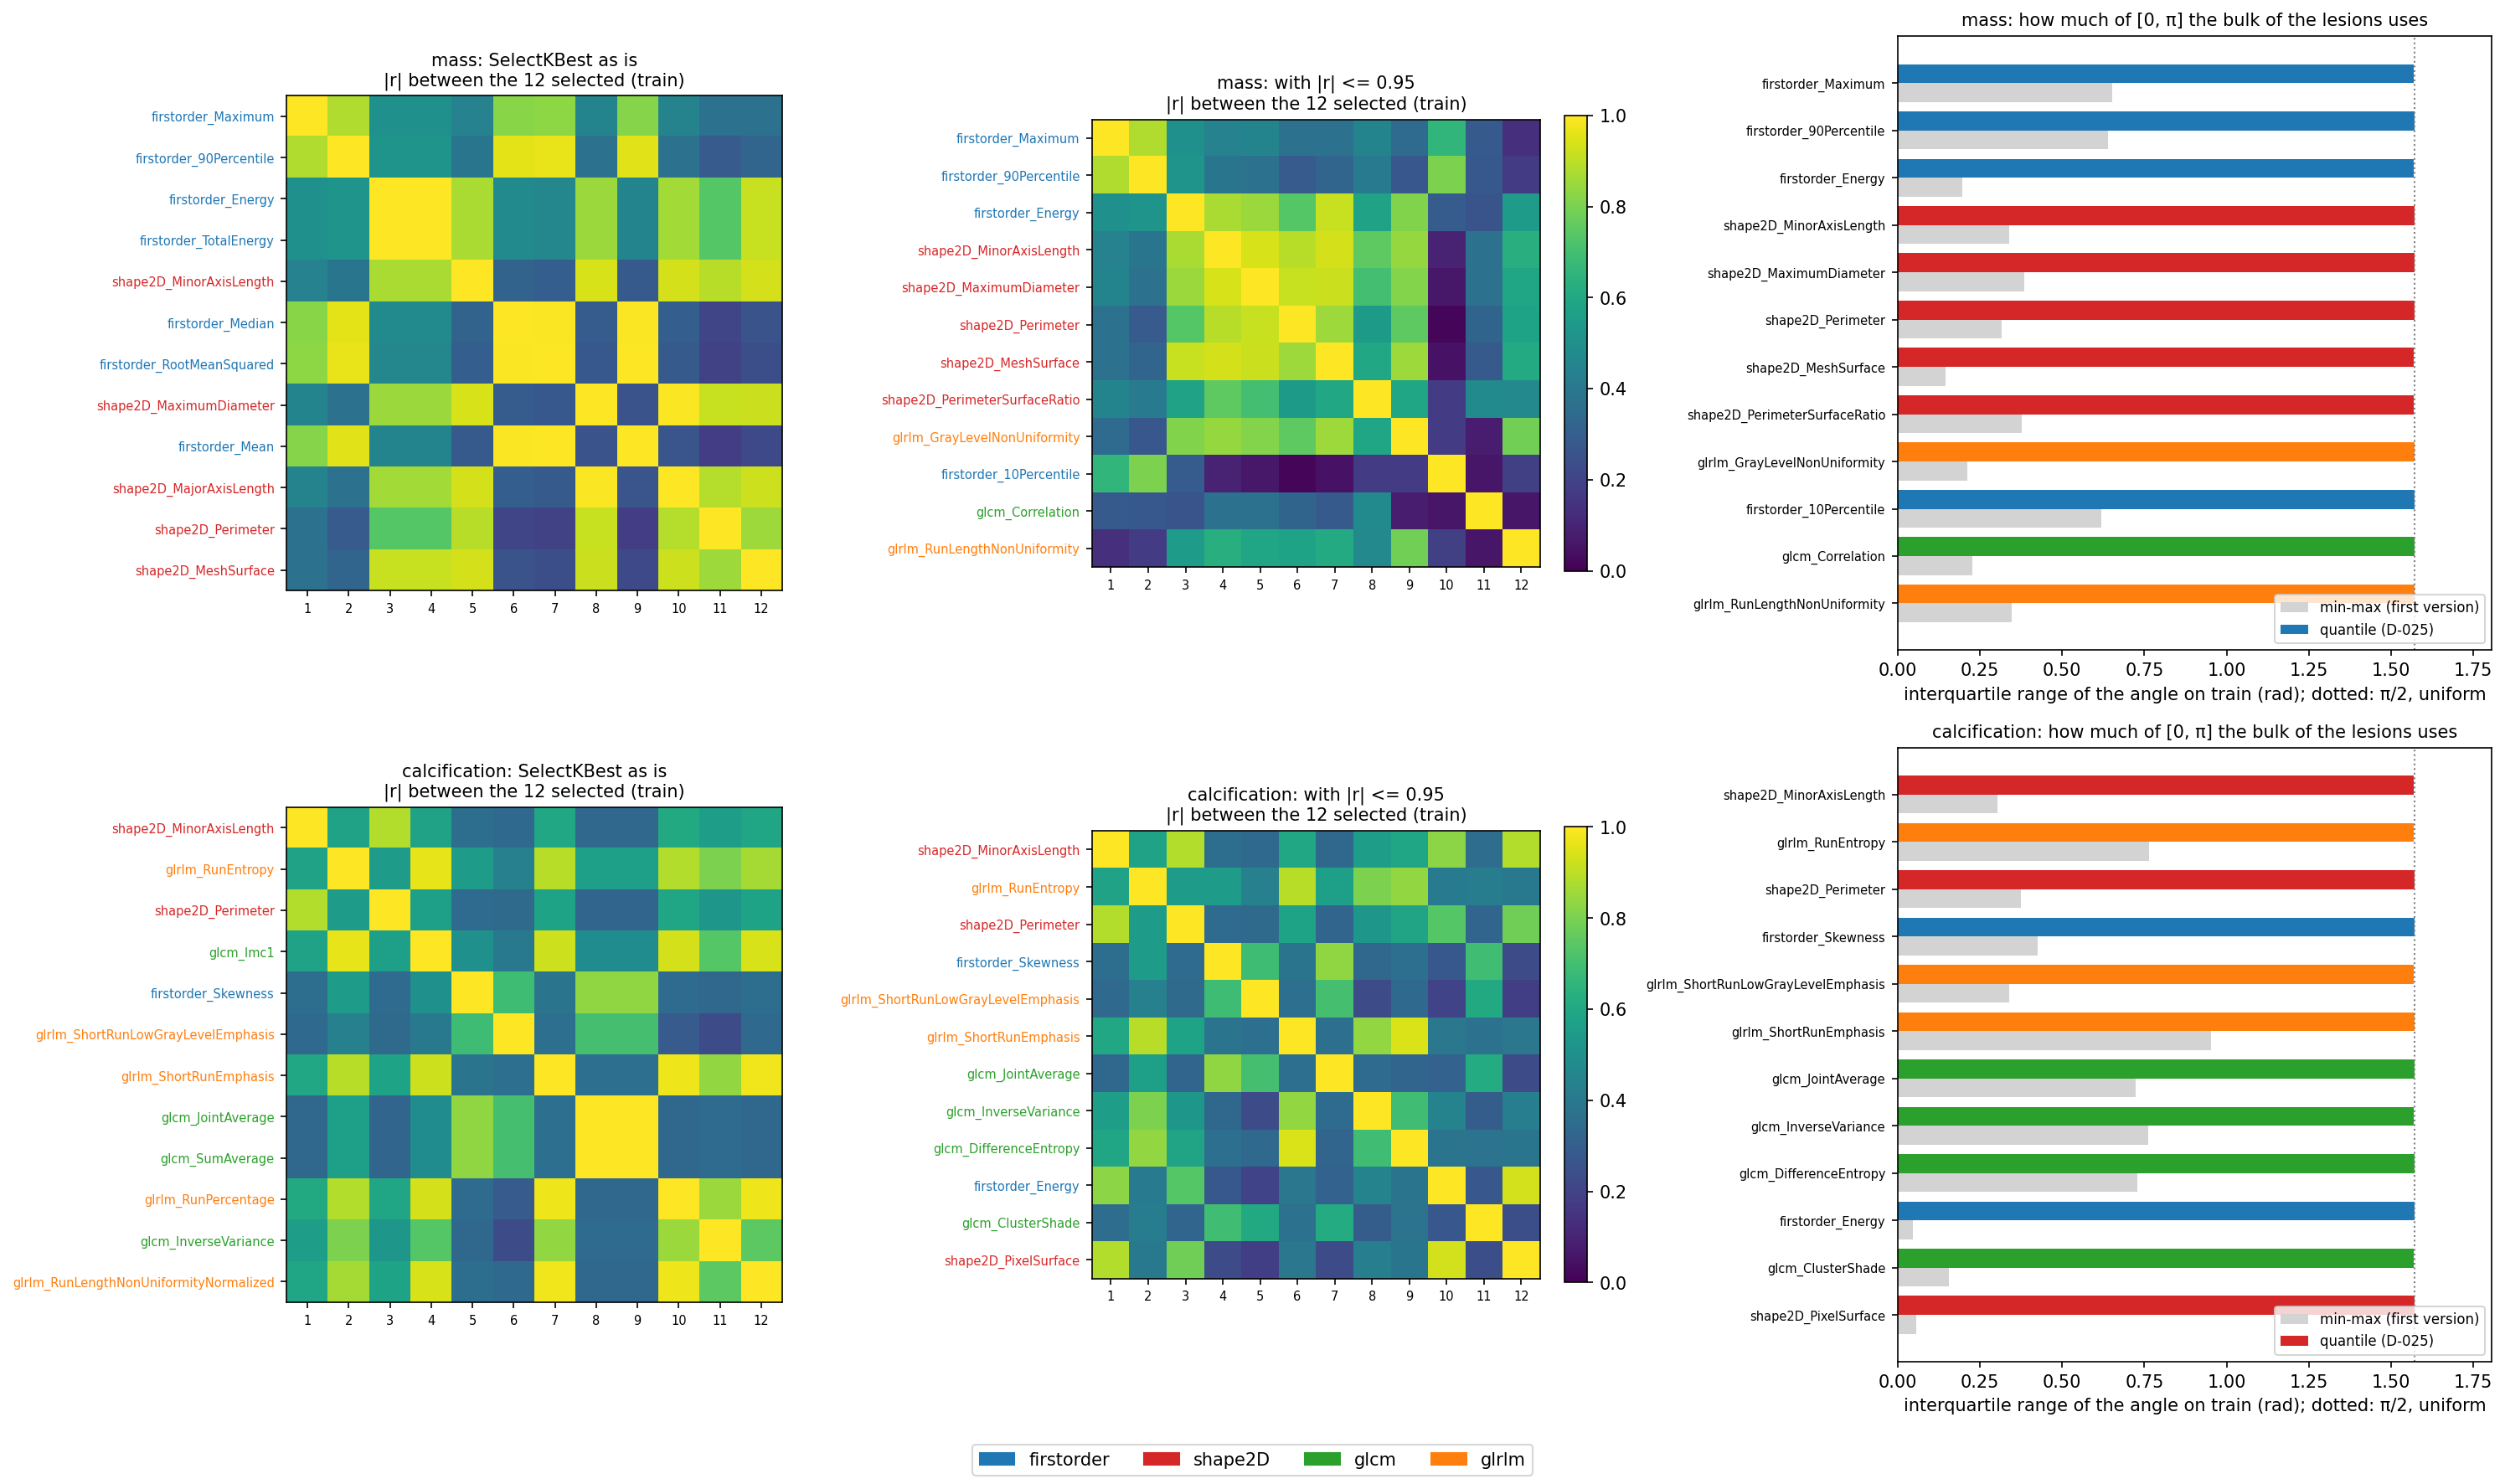
\includegraphics[width=\textwidth]{Figures/M4_selection_and_angles.png}
% fuente: H-026, H-028; 4_seleccion.csv
\caption{Distribución angular tras la selección de características y comparación entre escalado por valores extremos y transformación por cuantiles.}
\label{fig:m4_selection_angles}
\end{figure}

% fuente: H-035; X1_varianza_retenida.csv, X1_auc_por_condicion.csv, X1_auc_vs_k.csv
El análisis sobre la pérdida de información al reducir de 67 a 12 características reveló que
las variables seleccionadas retienen el 86.8\,\% de la varianza total en masas y el 90.2\,\% en calcificaciones,
frente al 98.0\,\% y 97.8\,\% alcanzable mediante las doce primeras componentes de un análisis de componentes
principales. En términos de capacidad predictiva sobre el conjunto de entrenamiento, la reducción a doce dimensiones
implicó una disminución de 2 a 4 puntos de AUC en modelos clásicos: en regresión logística, el AUC descendió
de $0.693 \pm 0.039$ a $0.650 \pm 0.056$ en masas y de $0.800 \pm 0.028$ a $0.758 \pm 0.025$ en calcificaciones;
en bosques aleatorios, la variación fue de $0.695 \pm 0.043$ a $0.680 \pm 0.046$ en masas y de $0.796 \pm 0.018$
a $0.773 \pm 0.024$ en calcificaciones. Asimismo, doce características seleccionadas al azar obtuvieron desempeños
comparables ($0.656 \pm 0.019$ y $0.659 \pm 0.023$ en masas; $0.765 \pm 0.015$ y $0.775 \pm 0.016$ en calcificaciones),
ilustrando que las variables con mayor puntuación univariante individual no necesariamente configuran el conjunto
óptimo debido a redundancias en la información compartida \cite{Guyon2003} (figura~\ref{fig:x1_selection_auc_vs_k}).

\begin{figure}[htbp]
\centering
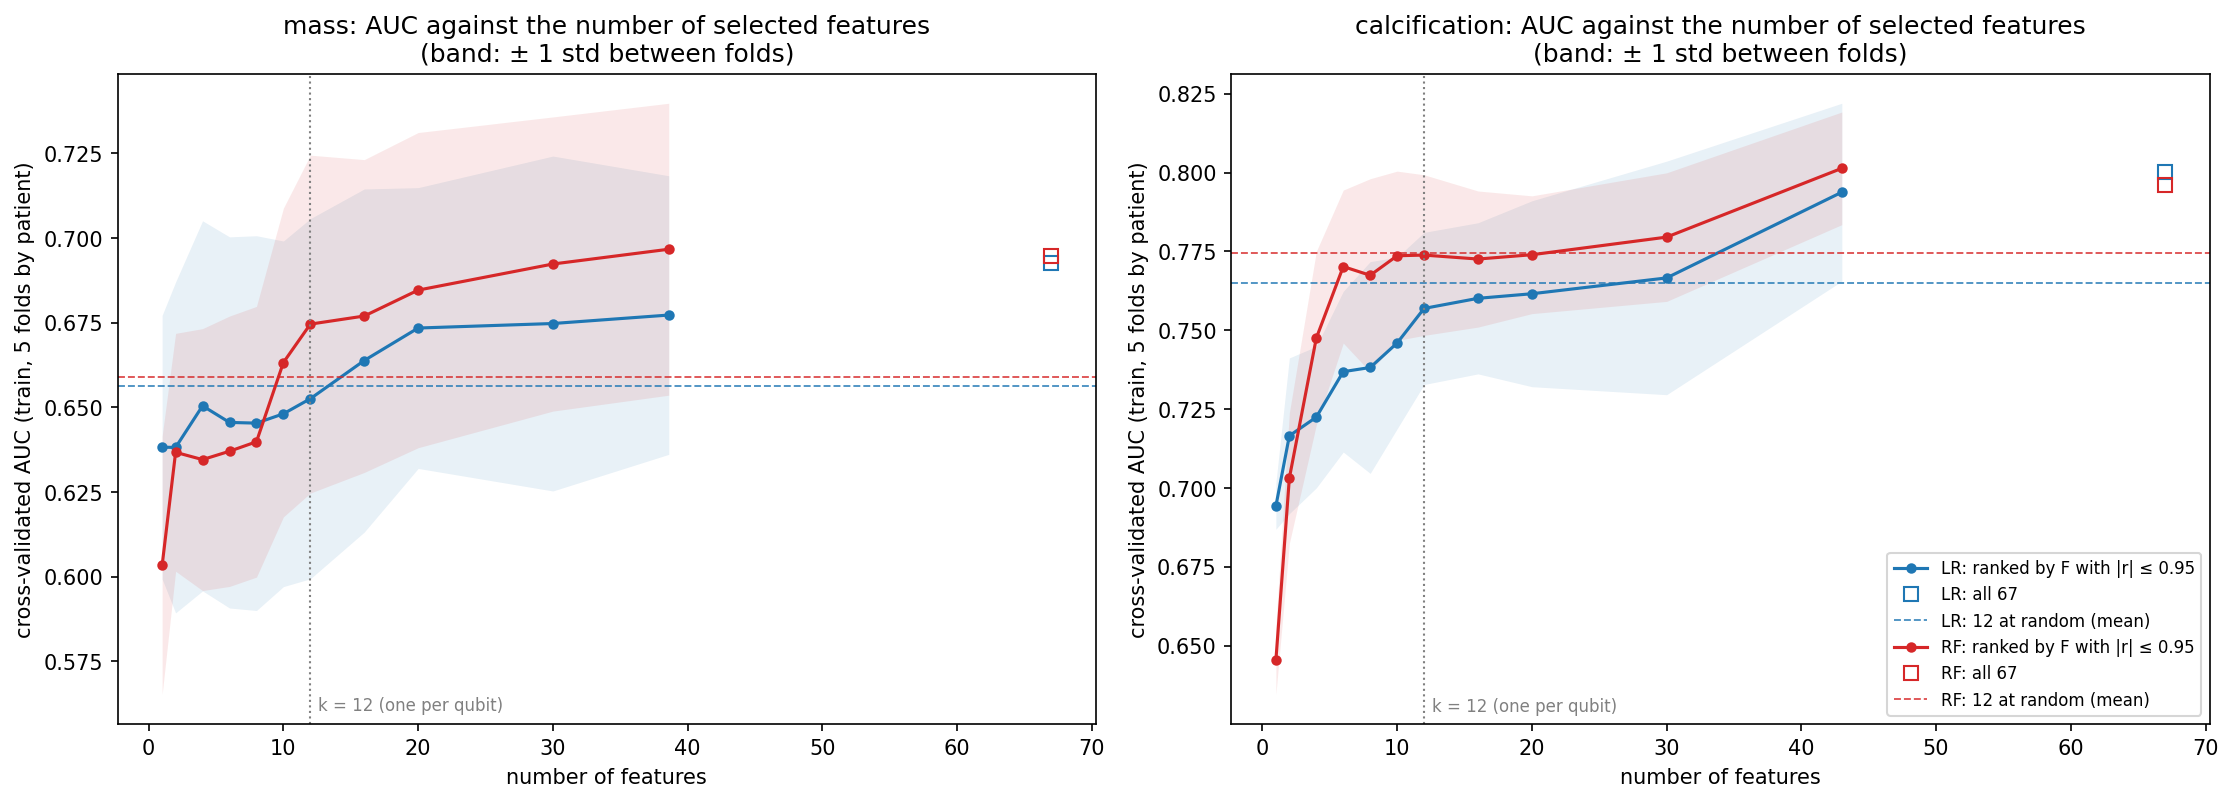
\includegraphics[width=\textwidth]{Figures/X1_selection_auc_vs_k.png}
% fuente: H-035; X1_auc_vs_k.csv
\caption{Evolución del área bajo la curva ROC en función del número de características $k$ para modelos clásicos en entrenamiento.}
\label{fig:x1_selection_auc_vs_k}
\end{figure}

% fuente: H-030, H-035
Esta limitación intrínseca de la selección univariante introduce una consideración metodológica central que matiza la comparación:
el criterio de \texttt{SelectKBest} evalúa cada variable de forma aislada mediante la prueba F de ANOVA, mientras que el filtro de
redundancia examina correlaciones lineales dos a dos. Como consecuencia, aquellas características cuyo poder discriminativo dependa
exclusivamente de interacciones de orden superior con otras variables (como en configuraciones de tipo o-exclusivo) resultan
descartadas antes de alimentar el circuito cuántico. Esta dinámica genera una tensión conceptual con el diseño experimental, puesto que
el bloque de acoplamiento $ZZ$ del mapa de características codifica precisamente productos de pares $(\pi - x_i)(\pi - x_j)$, que
constituyen el mecanismo primario mediante el cual la transformación cuántica podría aportar ventajas frente a representaciones clásicas.
Aunque la comparación entre las cinco condiciones se mantiene metodológicamente rigurosa al suministrar exactamente el mismo vector
de 12 características a todos los modelos, la ausencia de una selección multivariante capaz de capturar interacciones complejas
representa una restricción de diseño que contextualiza los resultados y explica por qué la selección guiada por F no supera de forma
concluyente a selecciones aleatorias en el experimento X1.

% ---
% Reemplaza parte de la sección de resultados en Docs/Technical_Report.tex.
% Entradas que lo respaldan: H-018, H-019, H-031, H-036, H-037, H-038, H-039, H-040, H-041, H-055, D-029, D-033, D-042.
% ---

\subsection{Separabilidad de las representaciones}
\label{sec:separabilidad_representaciones}

% fuente: H-031, H-037; 5a_resumen.csv, 5b_concentracion_kernel.csv
En la evaluación del kernel cuántico de fidelidad a escala nominal ($c = 1$) sobre la submuestra
estratificada de 200 lesiones de entrenamiento por subconjunto, las matrices de similitud resultaron
cercanas a la identidad. En masas, la mediana fuera de la diagonal fue de 0.0022 en C4 (con percentil 95
de 0.011 y 23\,\% de pares con fidelidad inferior a $10^{-3}$) y de 0.000032 en C5 (con 80\,\% de pares
por debajo de $10^{-3}$ y 26\,\% por debajo de $10^{-6}$). En calcificaciones, la mediana fue de 0.0029
en C4 (percentil 95 de 0.014 y 16\,\% bajo $10^{-3}$) y de 0.000031 en C5 (76\,\% bajo $10^{-3}$ y 28\,\%
bajo $10^{-6}$). En contraste, el kernel clásico gaussiano RBF con parámetro $\gamma$ determinado por la
heurística de la mediana registró una mediana fuera de la diagonal de 0.607 en ambos subconjuntos.

% fuente: H-037; X3_comparacion_k8_k12.csv (family «B, embeddings (full train)», k = 12).
% Corregido el 2026-10-19 (auditoría A2-2): 0.056 de 5a_resumen.csv es sobre las 1,696 masas
% (entrenamiento y prueba); sobre el entrenamiento es 0.058, como en la tabla de esta sección.
Sobre todas las lesiones del conjunto de entrenamiento (1\,318 masas y 1\,546 calcificaciones),
la desviación estándar media por dimensión de los valores esperados $\langle Z_i \rangle$ fue de 0.058
en masas y 0.048 en calcificaciones para C4, mientras que en C5 ascendió a 0.180 en masas y 0.178 en
calcificaciones. En C4 las compuertas aplicadas tras la capa inicial de Hadamard son diagonales, por lo
que el término propio en $Z$ añade una variación angular moderada frente a las fases de acoplamiento $ZZ$.
En C5, la rotación no diagonal en el eje $Y$ modifica directamente las amplitudes antes de la acción de
los términos $ZZ$, dispersando los valores esperados locales pero acentuando la ortogonalidad mutua en el
espacio de estados cuánticos y concentrando la fidelidad unas setenta veces más que en C4 \cite{Thanasilp2024}.

% fuente: H-018, H-019; B3_concentracion_embedding.csv
Esta concentración del \textit{embedding} reproduce el comportamiento caracterizado en el estudio B3
sobre la dispersión de los valores esperados $\langle Z_i \rangle$ (evaluada sobre 100 entradas y 10 sorteos de $\boldsymbol\theta$
con cálculo analítico exacto tras corregir la inyección de ruido en la referencia). Dicho análisis evidenció tres
patrones fundamentales: en primer lugar, la concentración con el número de qubits es sistemática, reduciéndose la dispersión media
a \texttt{reps} = 1 de $0.0837 \pm 0.0131$ con $k = 8$ a $0.0417 \pm 0.0068$ con $k = 12$ y a $0.0363 \pm 0.0090$ con $k = 16$,
comportamiento característico del crecimiento exponencial del espacio de Hilbert y precursor de las mesetas áridas (\textit{barren plateaus}).
En segundo lugar, la concentración con la profundidad del circuito no es monótona en el rango analizado: para $k = 12$, la dispersión
se incrementa en un 30\,\% al pasar de \texttt{reps} = 1 a \texttt{reps} = 2 ($0.0417 \pm 0.0068$ frente a $0.0544 \pm 0.0036$),
descendiendo a $0.0305 \pm 0.0044$ con \texttt{reps} = 3. En tercer lugar, la variabilidad entre distintos sorteos del vector $\boldsymbol\theta$
colapsa con la profundidad: a $k = 16$, la desviación entre sorteos se reduce de 0.0090 a 0.0043 y finalmente a 0.0023, reflejando
una pérdida progresiva de sensibilidad respecto a los parámetros del circuito que es indicativa del régimen de meseta árida.

\begin{figure}[htbp]
\centering
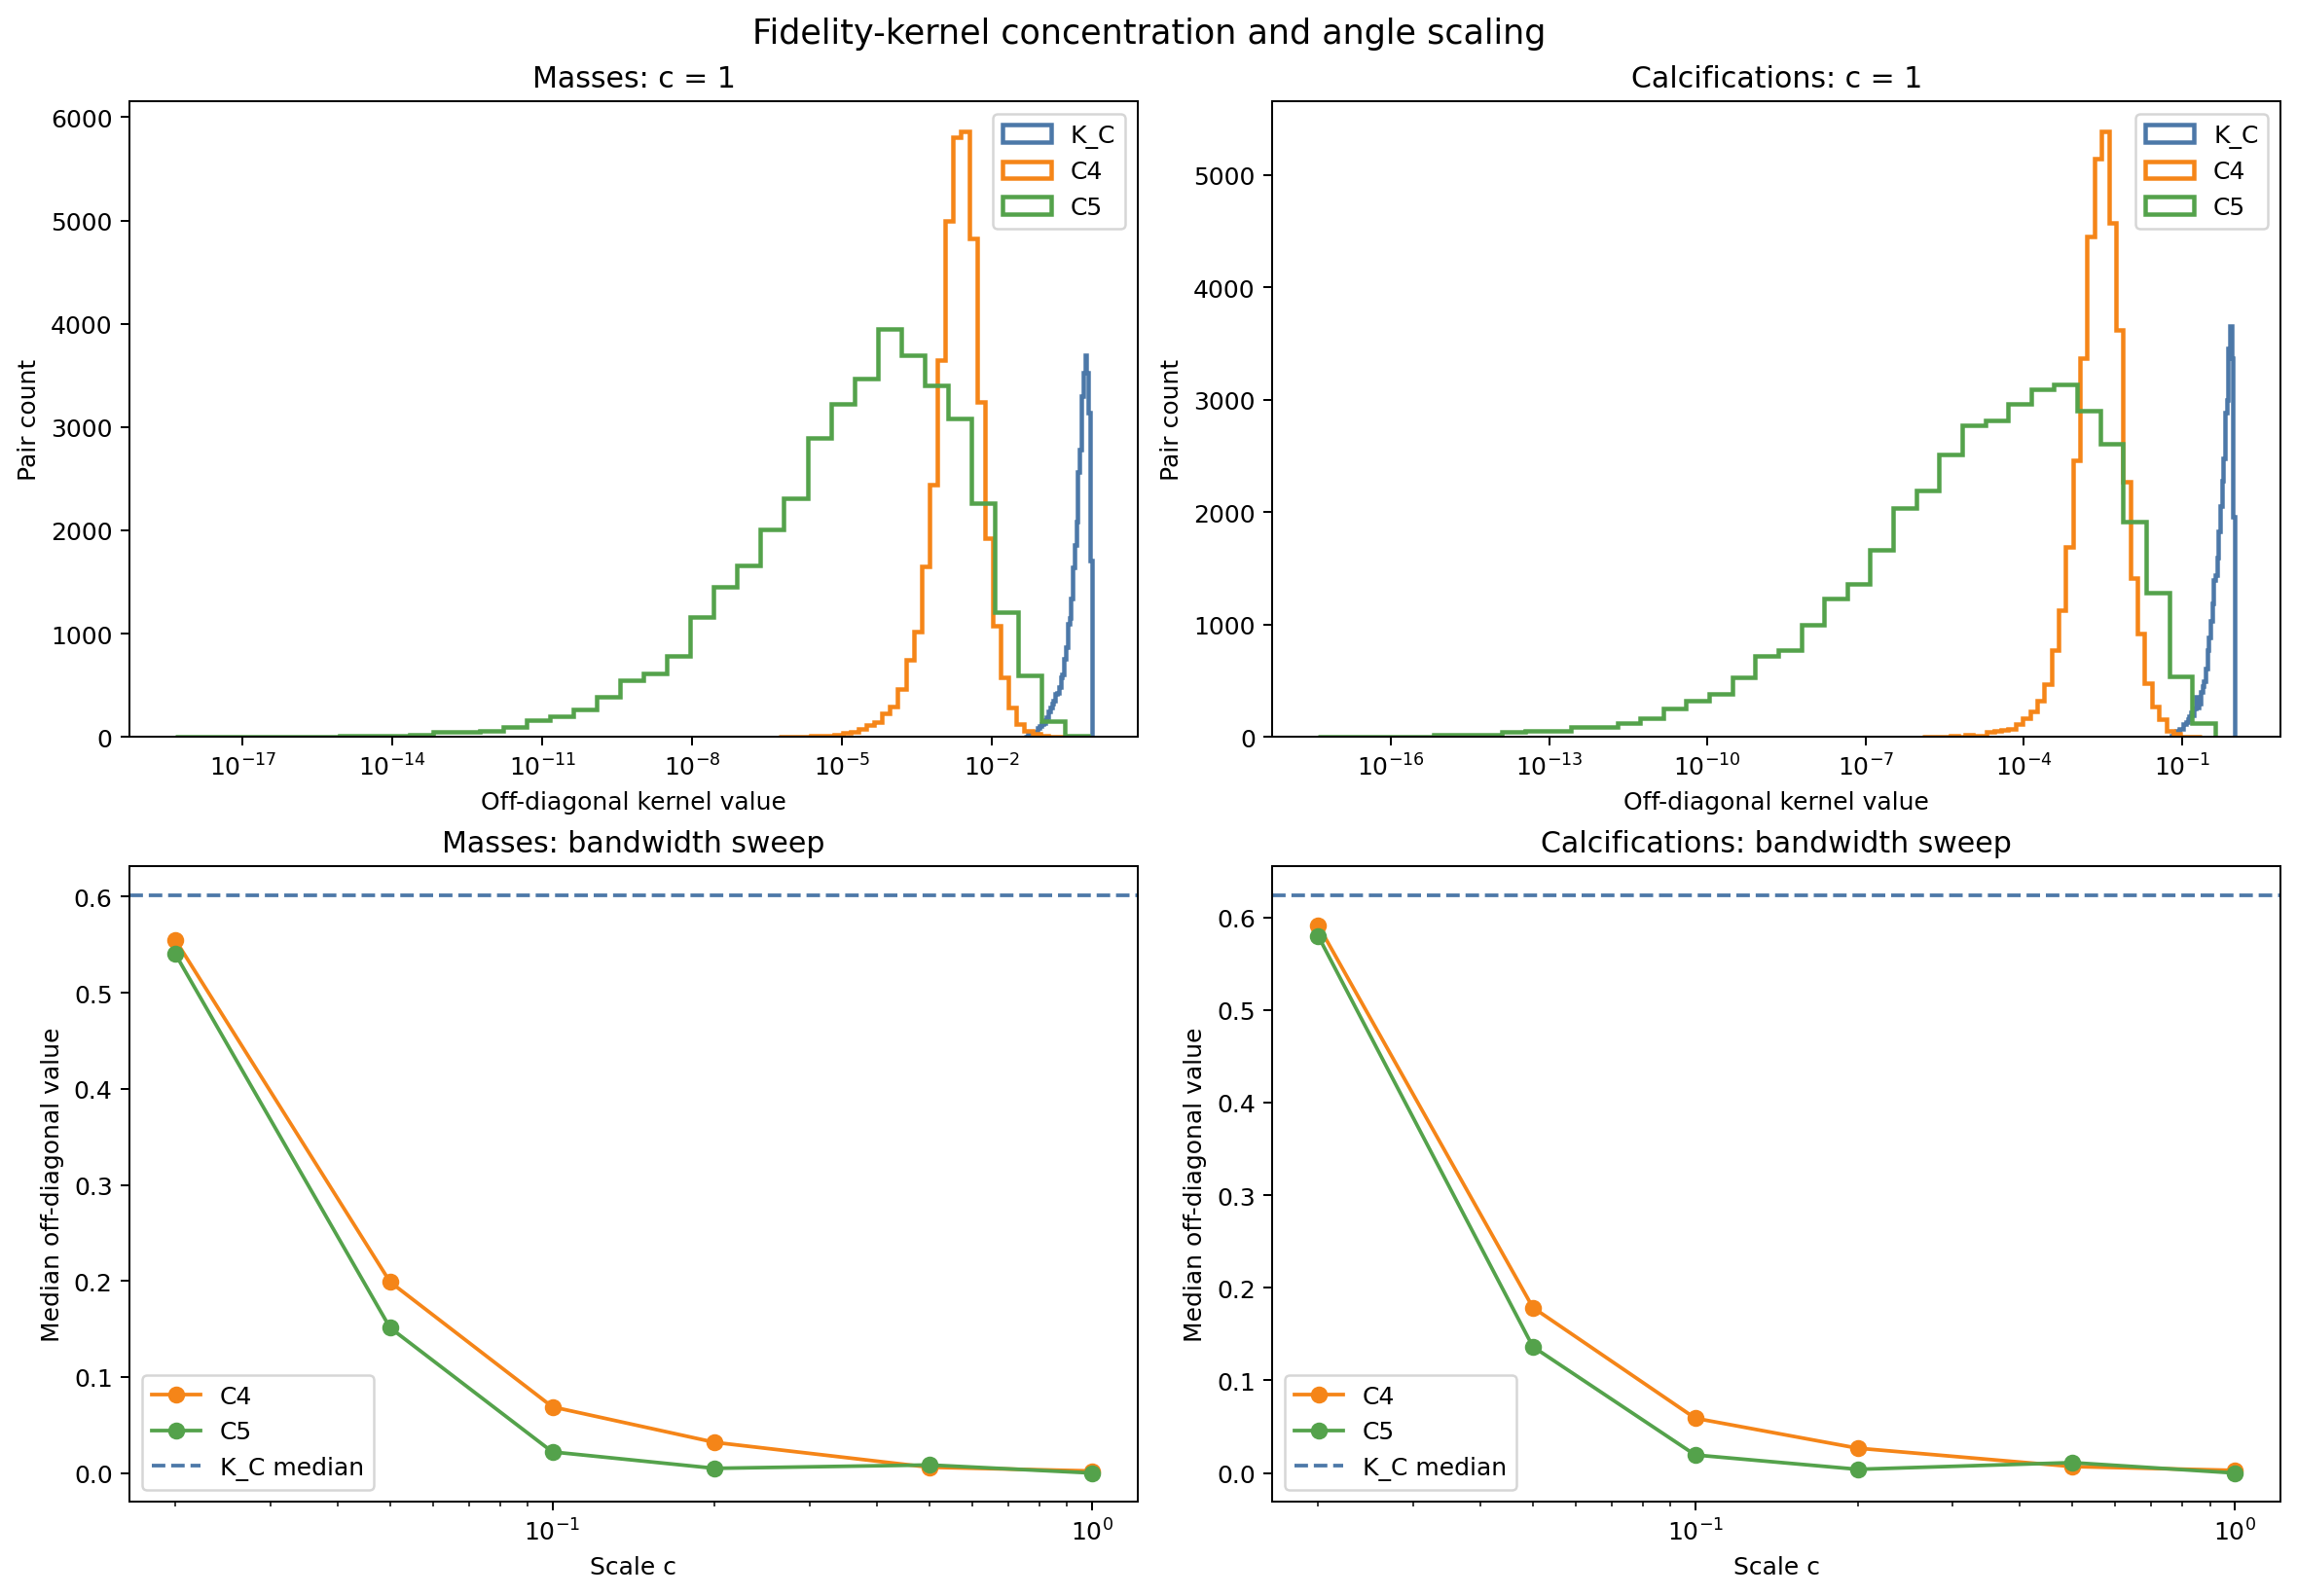
\includegraphics[width=\textwidth]{Figures/M5_kernel_concentration.png}
% fuente: H-031, H-037; 5b_concentracion_kernel.csv
\caption{Distribución de los valores fuera de la diagonal en las matrices de kernel cuántico para C4 y C5 frente al kernel clásico RBF.}
\label{fig:m5_kernel_concentration}
\end{figure}

% fuente: H-038, H-039; 6_alineamiento_kernel.csv, 6_dimension_efectiva.csv, 6_diferencia_geometrica_resumen.csv
Los resultados de separabilidad formal en la familia de kernels se resumen en la
Tabla~\ref{tab:m6_kernels}, calculados sobre la submuestra de entrenamiento con $c = 1$.

% fuente: H-038, H-039; 6_alineamiento_kernel.csv, 6_dimension_efectiva.csv, 6_diferencia_geometrica_resumen.csv
\input{tablas/m6_separabilidad_kernels}

% fuente: H-038, H-039; 6_alineamiento_kernel.csv
El exceso de alineamiento centrado (\textit{kernel-target alignment}, KTA) sobre la media de 1\,000
permutaciones de etiquetas fue en masas de 0.049 ($p < 0.001$) para el kernel clásico RBF, frente a 0.003
($p = 0.002$) en C4 y 0.005 ($p = 0.003$) en C5. En calcificaciones, el exceso del kernel RBF fue de 0.151
($p < 0.001$), frente a 0.006 ($p < 0.001$) en C4 y 0.007 ($p = 0.003$) en C5. Aunque el exceso en los
kernels cuánticos resultó estadísticamente significativo, representó únicamente entre el 4\,\% y el 10\,\%
del exceso clásico. Los valores absolutos de KTA centrada en C4 y C5 ($0.073$ a $0.077$) se encuentran
acotados por el valor base de $1/\sqrt{N-1} \approx 0.071$ inherente a matrices cercanas a la identidad
para muestras de $N = 200$ \cite{Cortes2012}.

% fuente: H-038, H-039; 6_dimension_efectiva.csv
La dimensión efectiva normalizada ($d_{\mathrm{eff}}$ de 200) arrojó 2.8 en masas y 2.6 en
calcificaciones para el kernel clásico RBF. Para los kernels cuánticos, los valores fueron de 184.0 en C4
y 171.3 en C5 para masas, y de 187.7 en C4 y 167.6 en C5 para calcificaciones. Las representaciones
cuánticas ocupan casi la totalidad de las dimensiones del espacio disponible ($d_{\mathrm{eff}} \approx N$),
régimen en el cual las cotas teóricas de error de generalización derivadas por Huang et al. \cite{huang2021power}
se aproximan a su valor máximo al escalar con $\sqrt{\min(d_{\mathrm{eff}}, \operatorname{Tr}(O^2))/N}$.

% fuente: H-038, H-039; 6_diferencia_geometrica_resumen.csv
En la métrica de diferencia geométrica regularizada frente a la batería de kernels clásicos,
los valores mínimos obtenidos fueron $g = 1.433$ en C4 y $1.511$ en C5 para masas, y $g = 1.400$ en C4
y $1.701$ en C5 para calcificaciones. En comparación con la cota de referencia $\sqrt{N} \approx 14.1$,
se cumple de forma consistente la condición $g \ll \sqrt{N}$, bajo la cual el marco teórico de Huang et al.
\cite{huang2021power} indica que los modelos clásicos pueden igualar o mejorar el desempeño del modelo cuántico
con cualquier vector de etiquetas. En la batería clásica extendida con gaussianos estrechos, el valor mínimo
se reduce a 1.31 en C4 y 1.48 en C5 para masas, y a 1.38 en C4 y 1.70 en C5 para calcificaciones. Por el contrario,
el cálculo de $g$ sin regularizar genera valores entre 306 y 388 (próximos a la cota teórica de $K_Q = I$,
$1/\sqrt{\lambda_{\min}(K_C)} \approx 410$), producto del condicionamiento numérico de la matriz clásica invertida.

\begin{figure}[htbp]
\centering
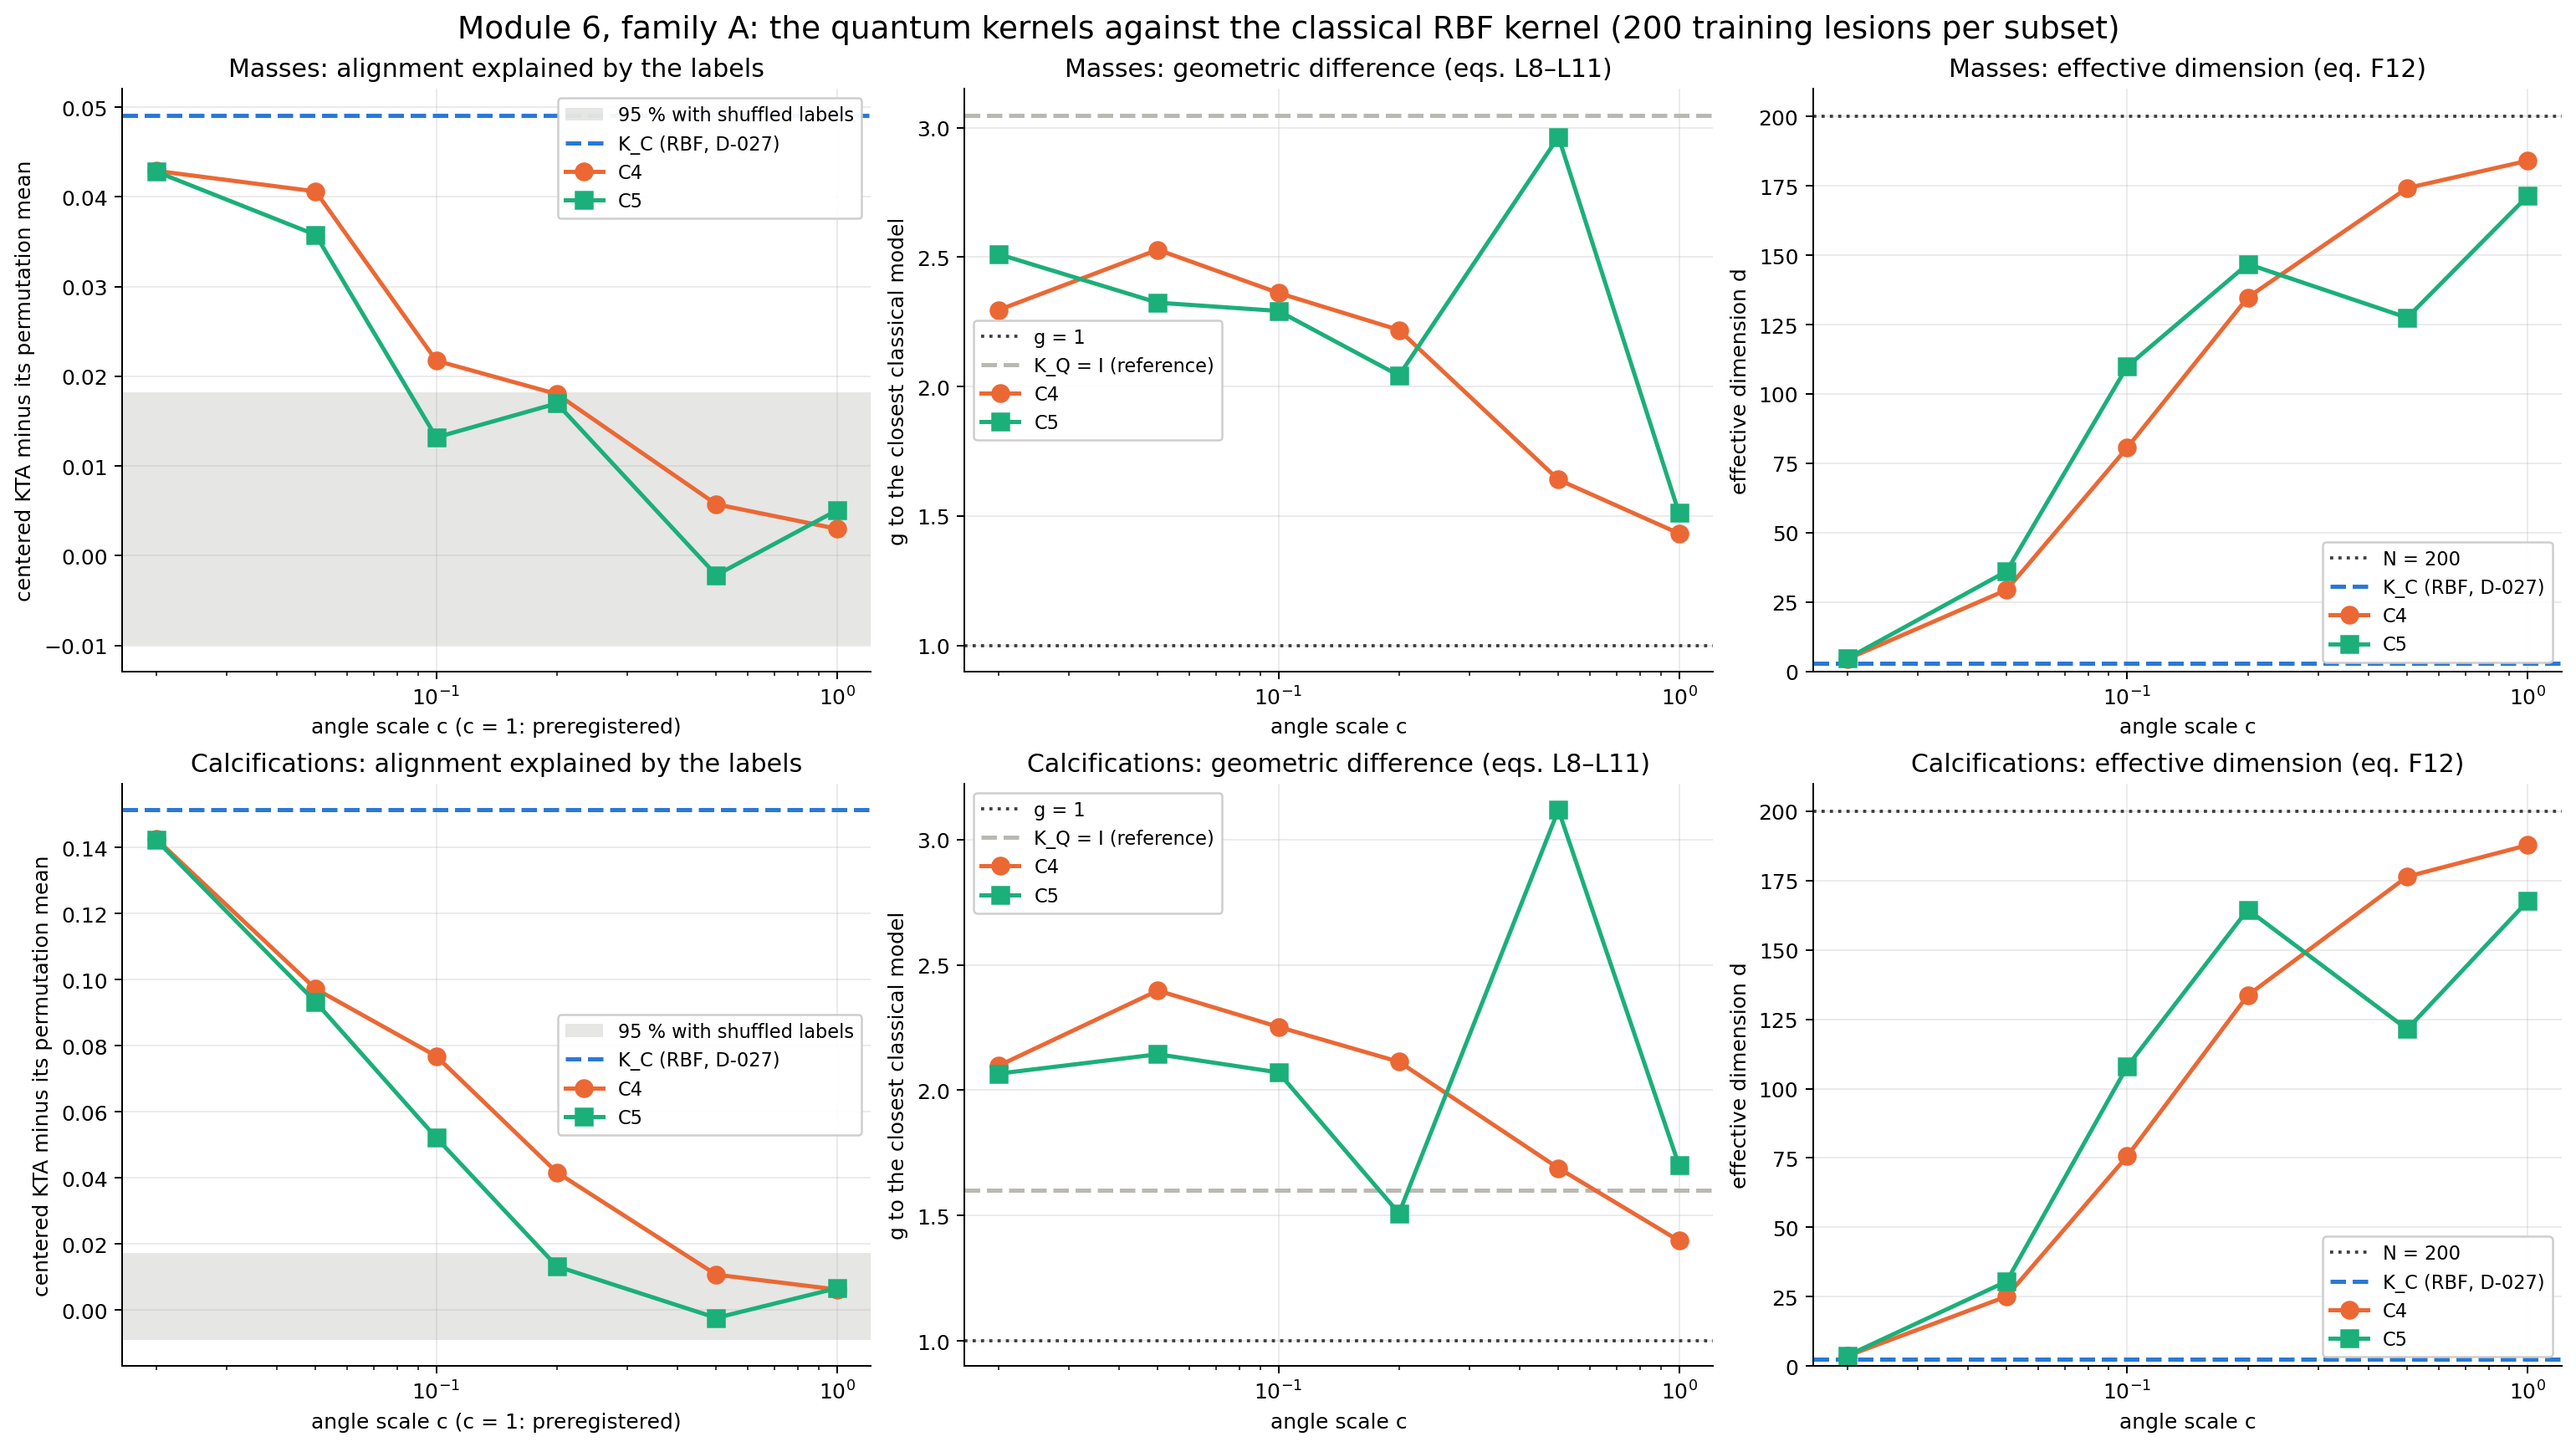
\includegraphics[width=\textwidth]{Figures/M6_kernel_metrics.png}
% fuente: H-038, H-039; 6_alineamiento_kernel.csv, 6_dimension_efectiva.csv
\caption{Métricas de separabilidad en la familia de kernels: alineamiento KTA y dimensión efectiva normalizada.}
\label{fig:m6_kernel_metrics}
\end{figure}

\begin{figure}[htbp]
\centering
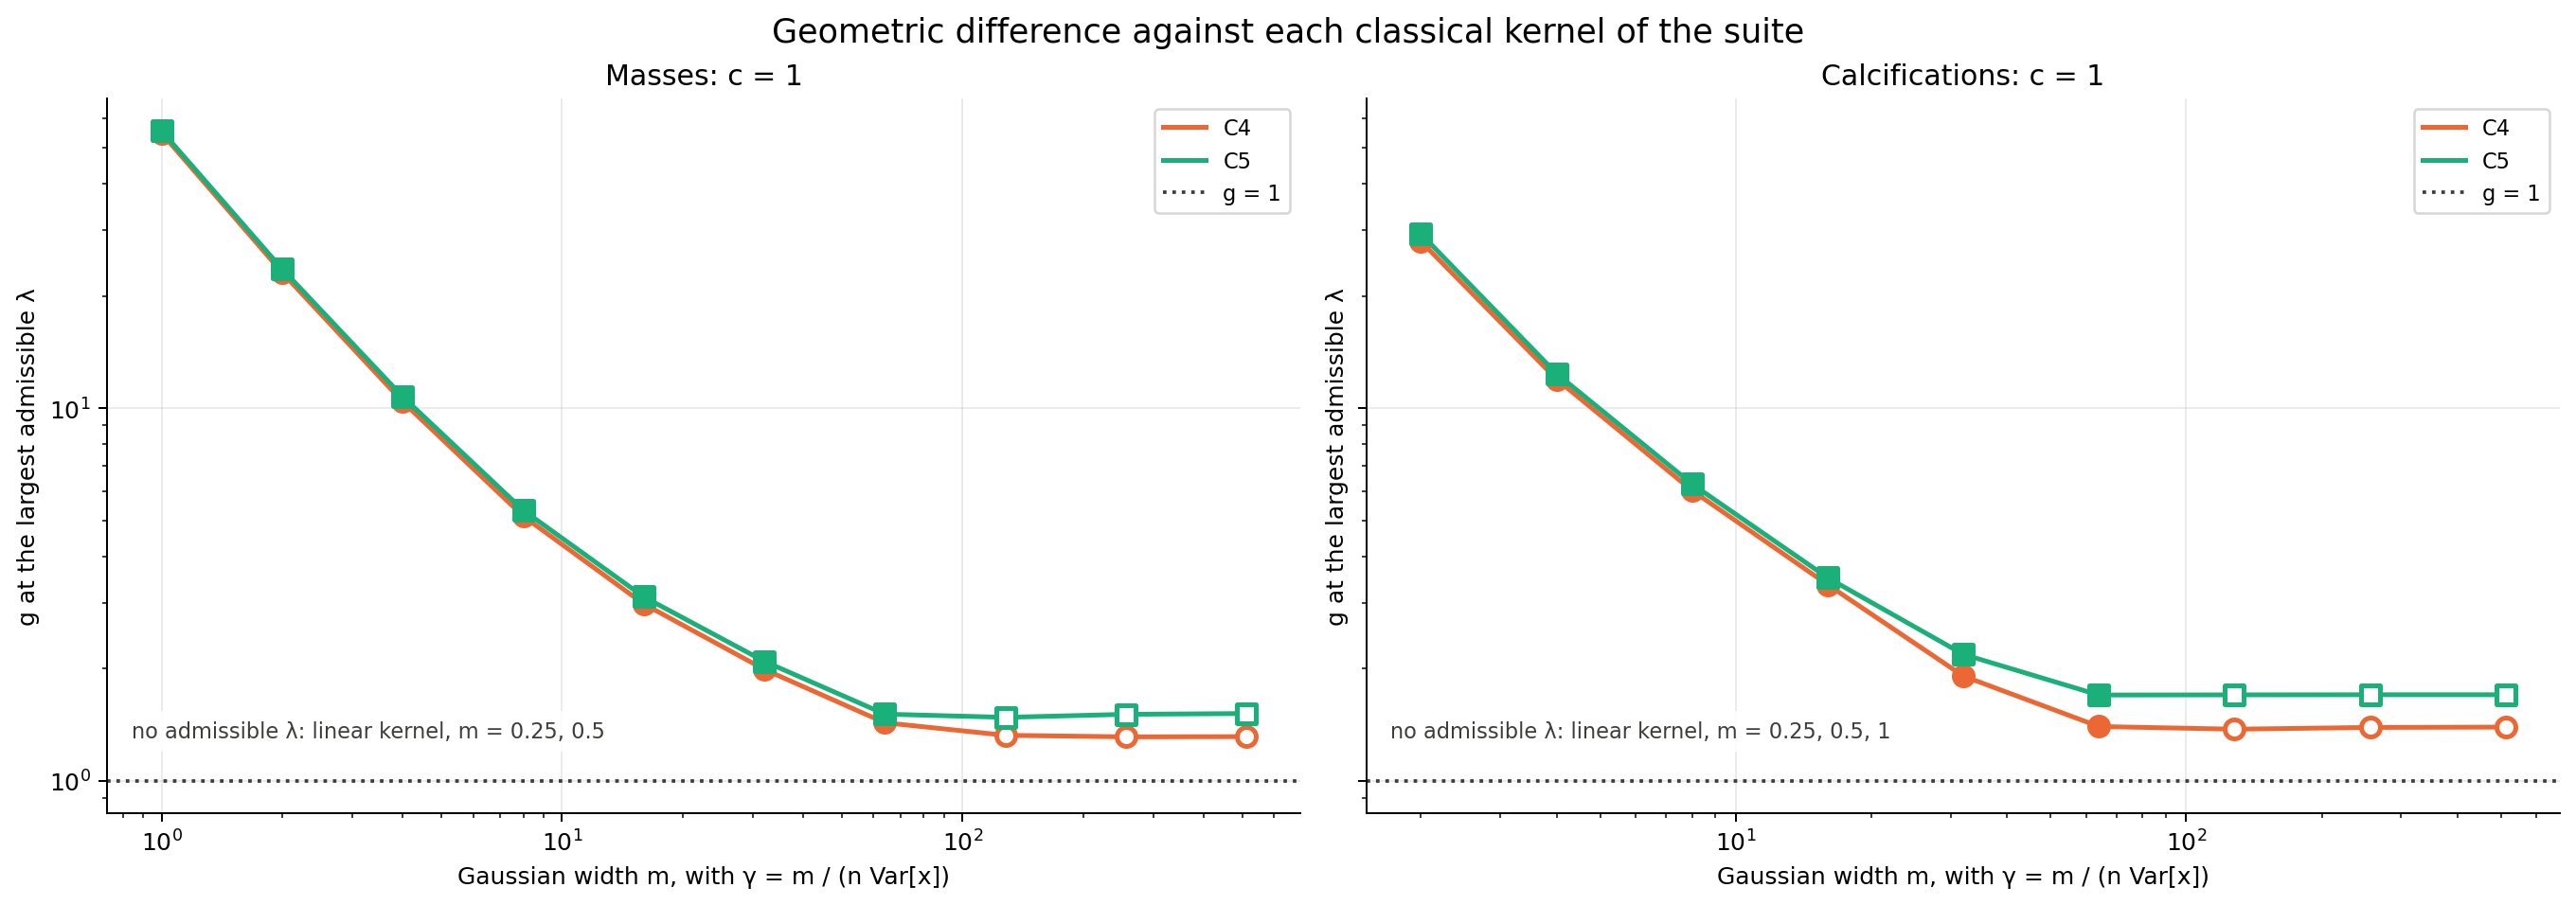
\includegraphics[width=\textwidth]{Figures/M6_geometric_difference.png}
% fuente: H-038, H-039; 6_diferencia_geometrica_resumen.csv
\caption{Diferencia geométrica regularizada $g$ respecto a la batería de modelos clásicos frente al límite $\sqrt{N}$.}
\label{fig:m6_geometric_difference}
\end{figure}

% fuente: H-040; 6_metricas_embedding.csv
La separabilidad sobre las representaciones vectoriales generadas por los cinco esquemas metodológicos
se presenta en la Tabla~\ref{tab:m6_embeddings}.

% fuente: H-040; 6_metricas_embedding.csv
\input{tablas/m6_separabilidad_embeddings}

% fuente: H-040; 6_metricas_embedding.csv
En la submuestra de 200 lesiones, las tres representaciones clásicas (C1, C2 y C3) superaron a las
cuánticas (C4 y C5) en todas las métricas evaluadas. En masas, el índice de Davies--Bouldin fue de 4.301 en C1
y C2 frente a 5.898 en C4 y 13.346 en C5 ($p = 0.41$); la razón de Fisher $J$ fue de 0.669 en C1 y C2 (y 0.781 en C3)
frente a 0.449 en C4 ($p = 0.05$) y 0.668 en C5; y el alineamiento lineal fue de 0.070 en C1 y C2 frente a 0.041 en C4
y 0.012 en C5 ($p = 0.41$). En calcificaciones, Davies--Bouldin fue de 2.387 en C1 y C2 frente a 6.890 en C4 y 6.247
en C5; Fisher $J$ fue de 1.284 en C1 y C2 (y 1.390 en C3) frente a 0.399 en C4 ($p = 0.15$) y 0.753 en C5; y el
alineamiento lineal fue de 0.181 en C1 y C2 frente a 0.031 en C4 y 0.041 en C5. Las métricas de C1 y C2 coincidieron
con discrepancias numéricas del orden del límite de precisión ($< 10^{-14}$), lo cual concuerda con la invarianza
teórica de las distancias y dispersiones ante rotaciones ortogonales bajo la condición de control nulo.
Al evaluar la razón de Fisher sobre la totalidad del conjunto de entrenamiento, la ventaja clásica se mantuvo:
C1 obtuvo 0.45 en masas y 1.06 en calcificaciones, frente a 0.13 y 0.42 en C4, y 0.21 y 0.31 en C5.

\begin{figure}[htbp]
\centering
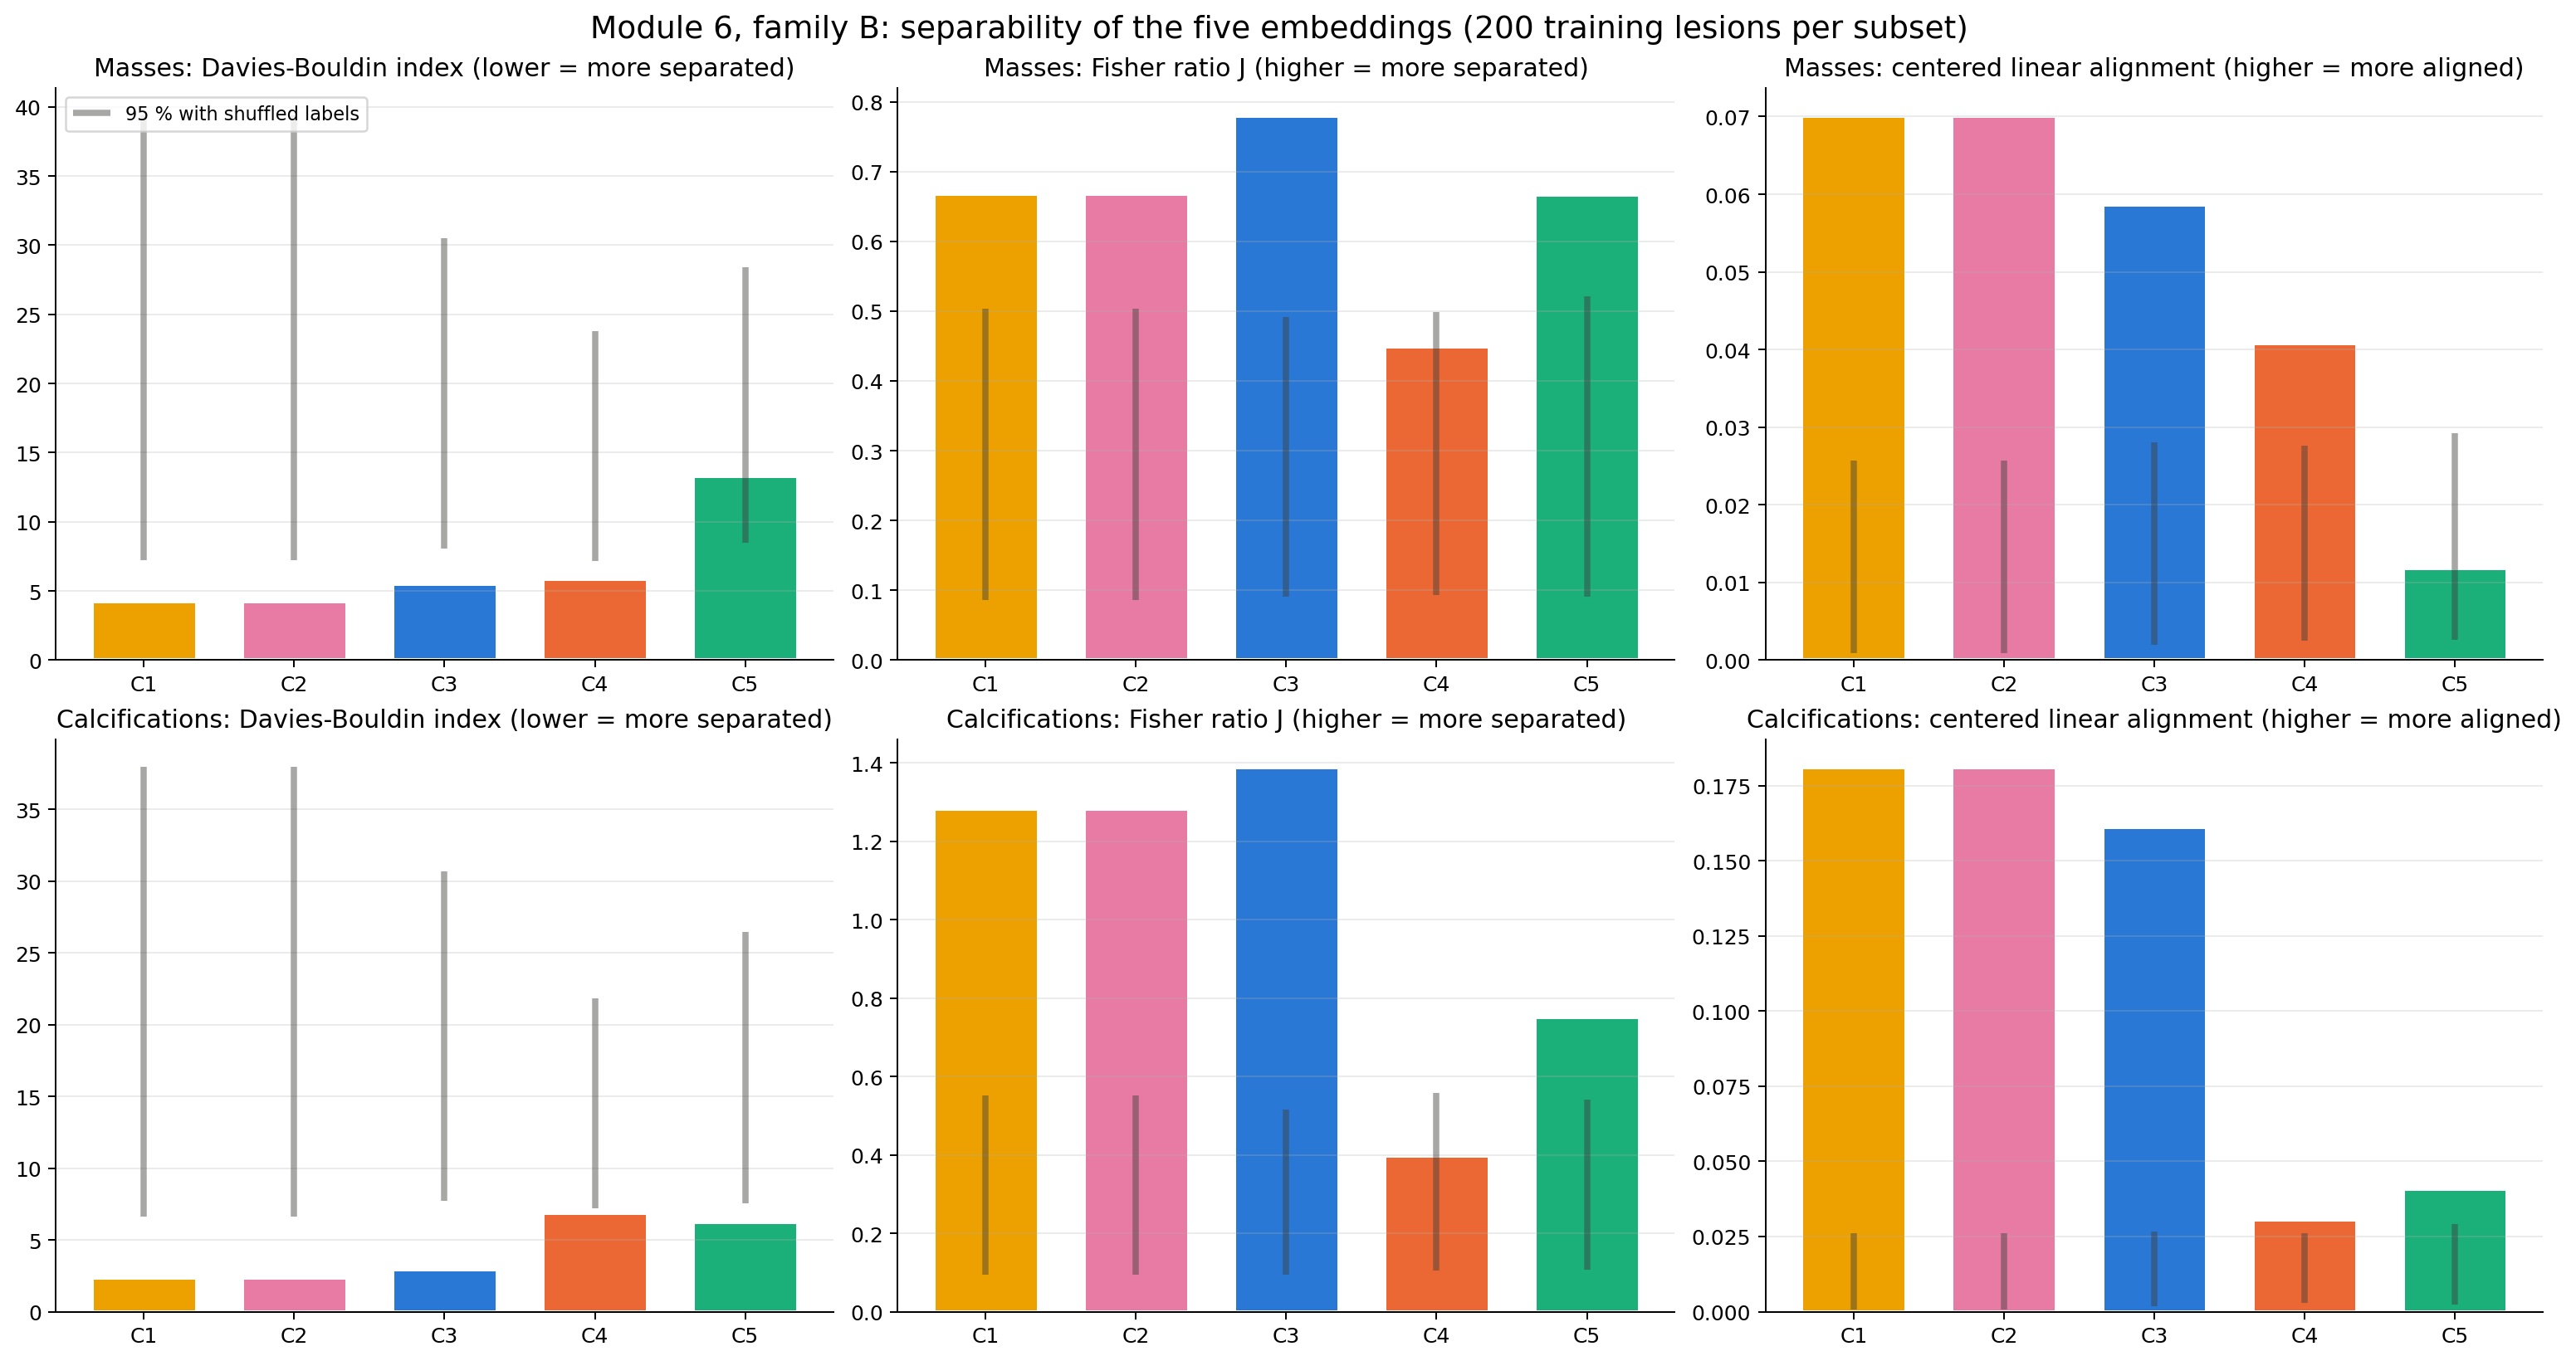
\includegraphics[width=\textwidth]{Figures/M6_embedding_metrics.png}
% fuente: H-040; 6_metricas_embedding.csv
\caption{Métricas de separabilidad sobre las representaciones vectoriales: índice de Davies--Bouldin, razón de Fisher y alineamiento lineal.}
\label{fig:m6_embedding_metrics}
\end{figure}

\begin{figure}[htbp]
\centering
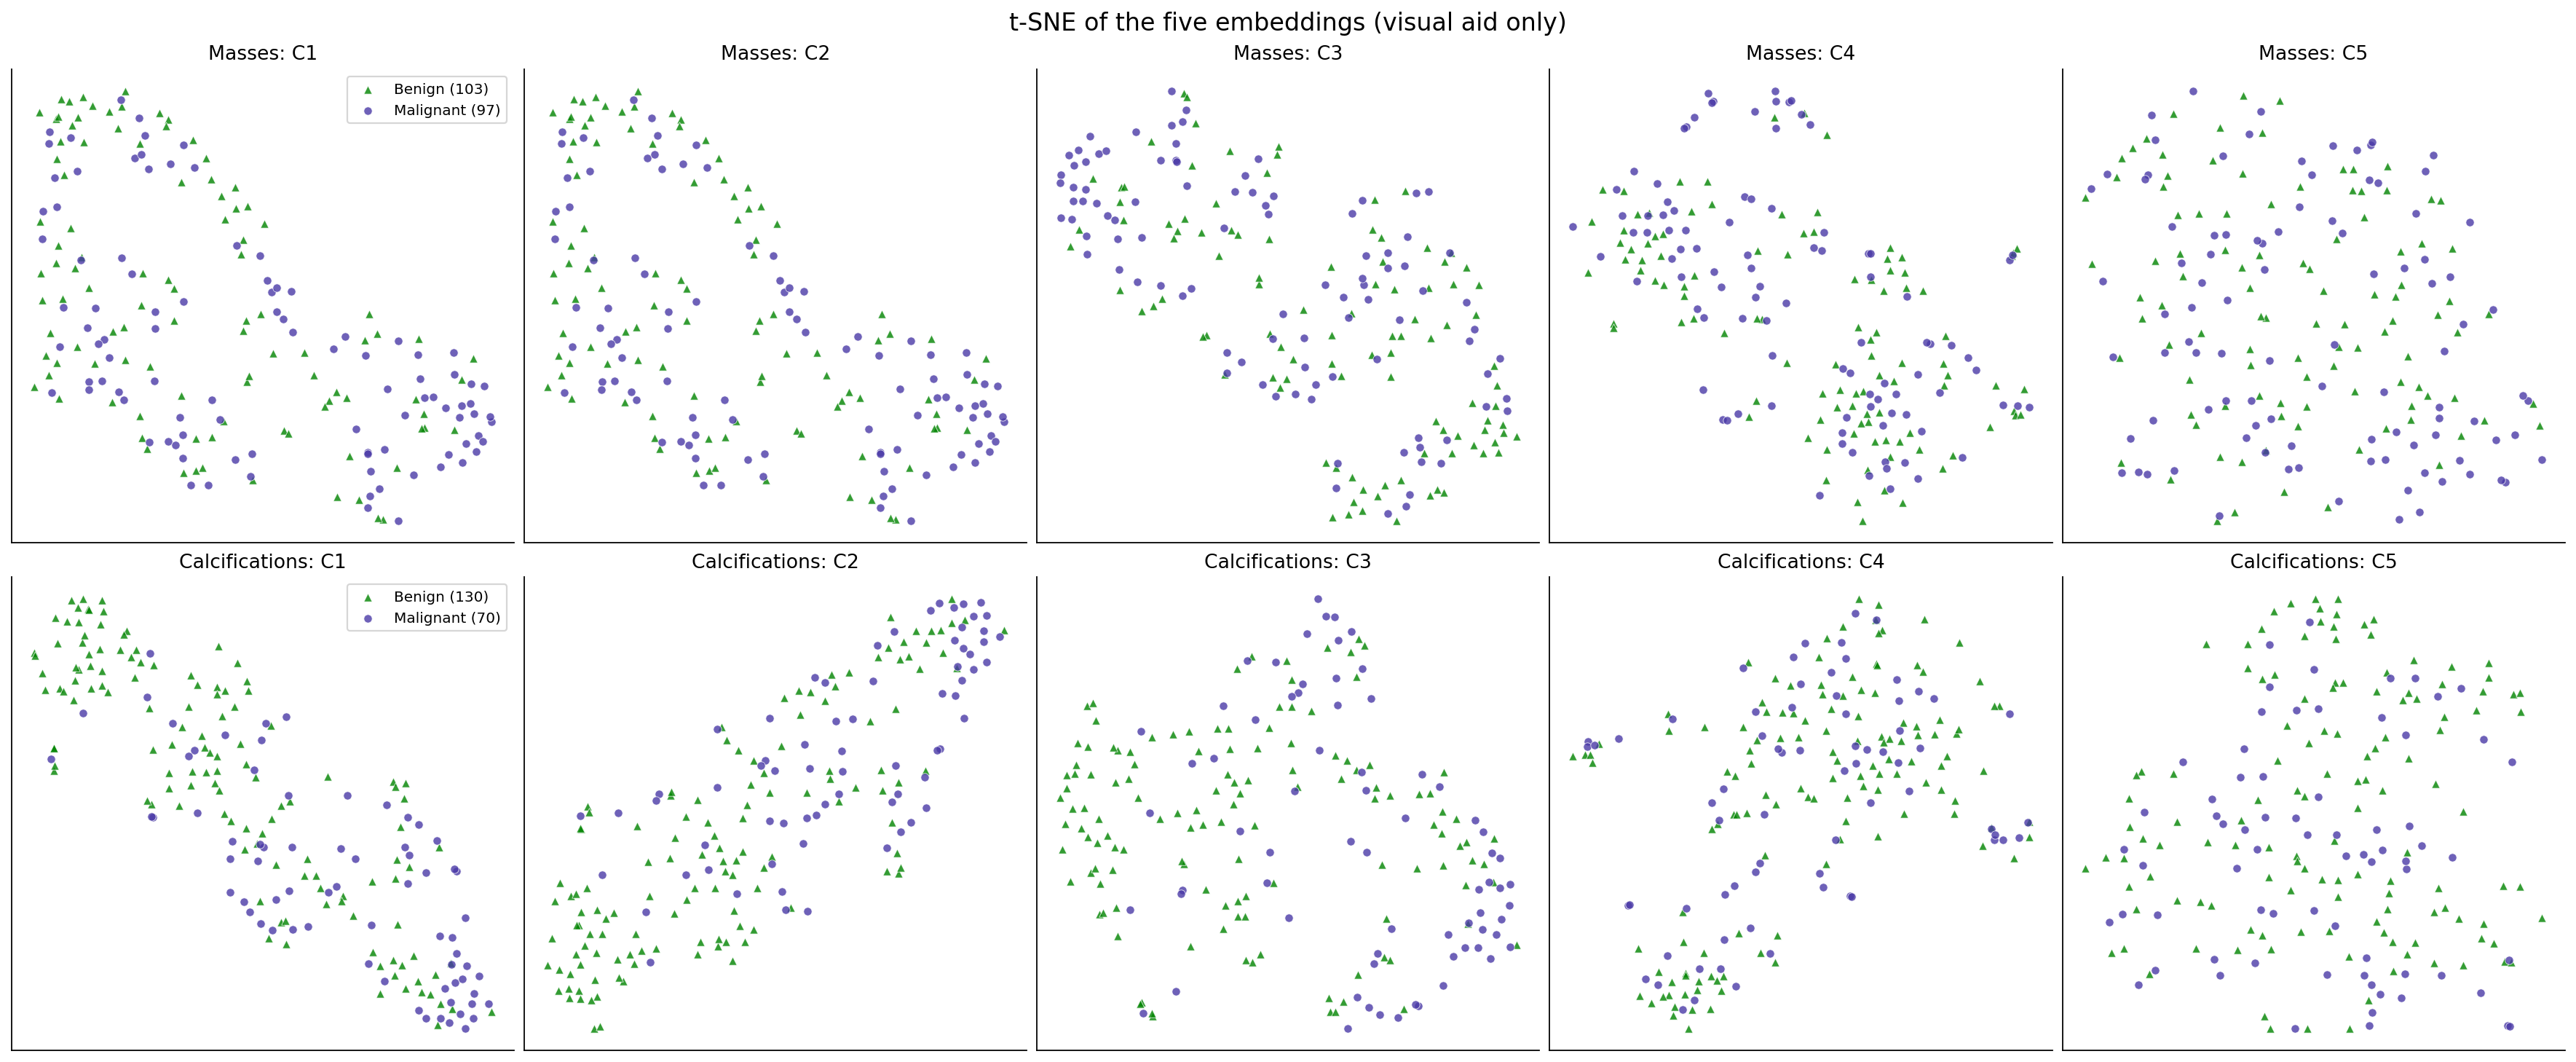
\includegraphics[width=\textwidth]{Figures/M6_tsne.png}
% fuente: H-040; 6_metricas_embedding.csv
\caption{Proyecciones bidimensionales mediante t-SNE para las representaciones generadas en las cinco condiciones.}
\label{fig:m6_tsne}
\end{figure}

% fuente: H-055, D-042; X9_resumen_familia_a.csv, X9_orden_familia_b.csv, X9_familia_a.csv
Para descartar que estas conclusiones dependan de la submuestra, las métricas a $c = 1$ se repitieron
sobre otras 19 submuestras estratificadas de 200 lesiones de entrenamiento y sobre la totalidad del
conjunto de entrenamiento, sin usar el conjunto de prueba (Figura~\ref{fig:x9_sample_size}). En las
20 submuestras de ambos subconjuntos, el kernel RBF conservó un exceso de KTA mayor que el de los dos
kernels cuánticos, sin traslape de rangos: el menor exceso clásico, 0.019 en masas y 0.055 en
calcificaciones, superó al mayor exceso cuántico, 0.011 y 0.014. La diferencia geométrica mínima se
mantuvo entre 1.31 y 2.87, a lo sumo 0.20 veces $\sqrt{N}$, y la dimensión efectiva de C4 y C5, entre
0.82 y 0.95 veces $N$. En las representaciones vectoriales, la mejor condición clásica (C1 o C3) superó
a las dos cuánticas en las 20 submuestras y en las tres métricas. Sobre todo el entrenamiento
(1\,318 masas y 1\,546 calcificaciones), el exceso de KTA fue de 0.055 para el RBF frente a 0.006 (C4)
y 0.009 (C5) en masas, y de 0.148 frente a 0.018 y 0.020 en calcificaciones, con $p = 0.001$ en todos
los casos; $g$ se ubicó entre 2.95 y 3.25, frente a $\sqrt{N}$ de 36.3 y 39.3. El exceso cuántico
crece con $N$ porque en un kernel concentrado la señal de clase reside en los $N(N-1)$ pares fuera de
la diagonal, cada uno con un traslape mínimo; por ello los valores de alineamiento, $g$ y dimensión
efectiva solo se comparan entre condiciones con el mismo $N$. Dos aspectos sí dependen de la muestra:
la significancia de los efectos más pequeños, pues C5 en masas llegó a $p = 0.24$ en alguna submuestra,
y el orden entre C4 y C5, que cambia con la métrica y con la submuestra.

\begin{figure}[htbp]
\centering
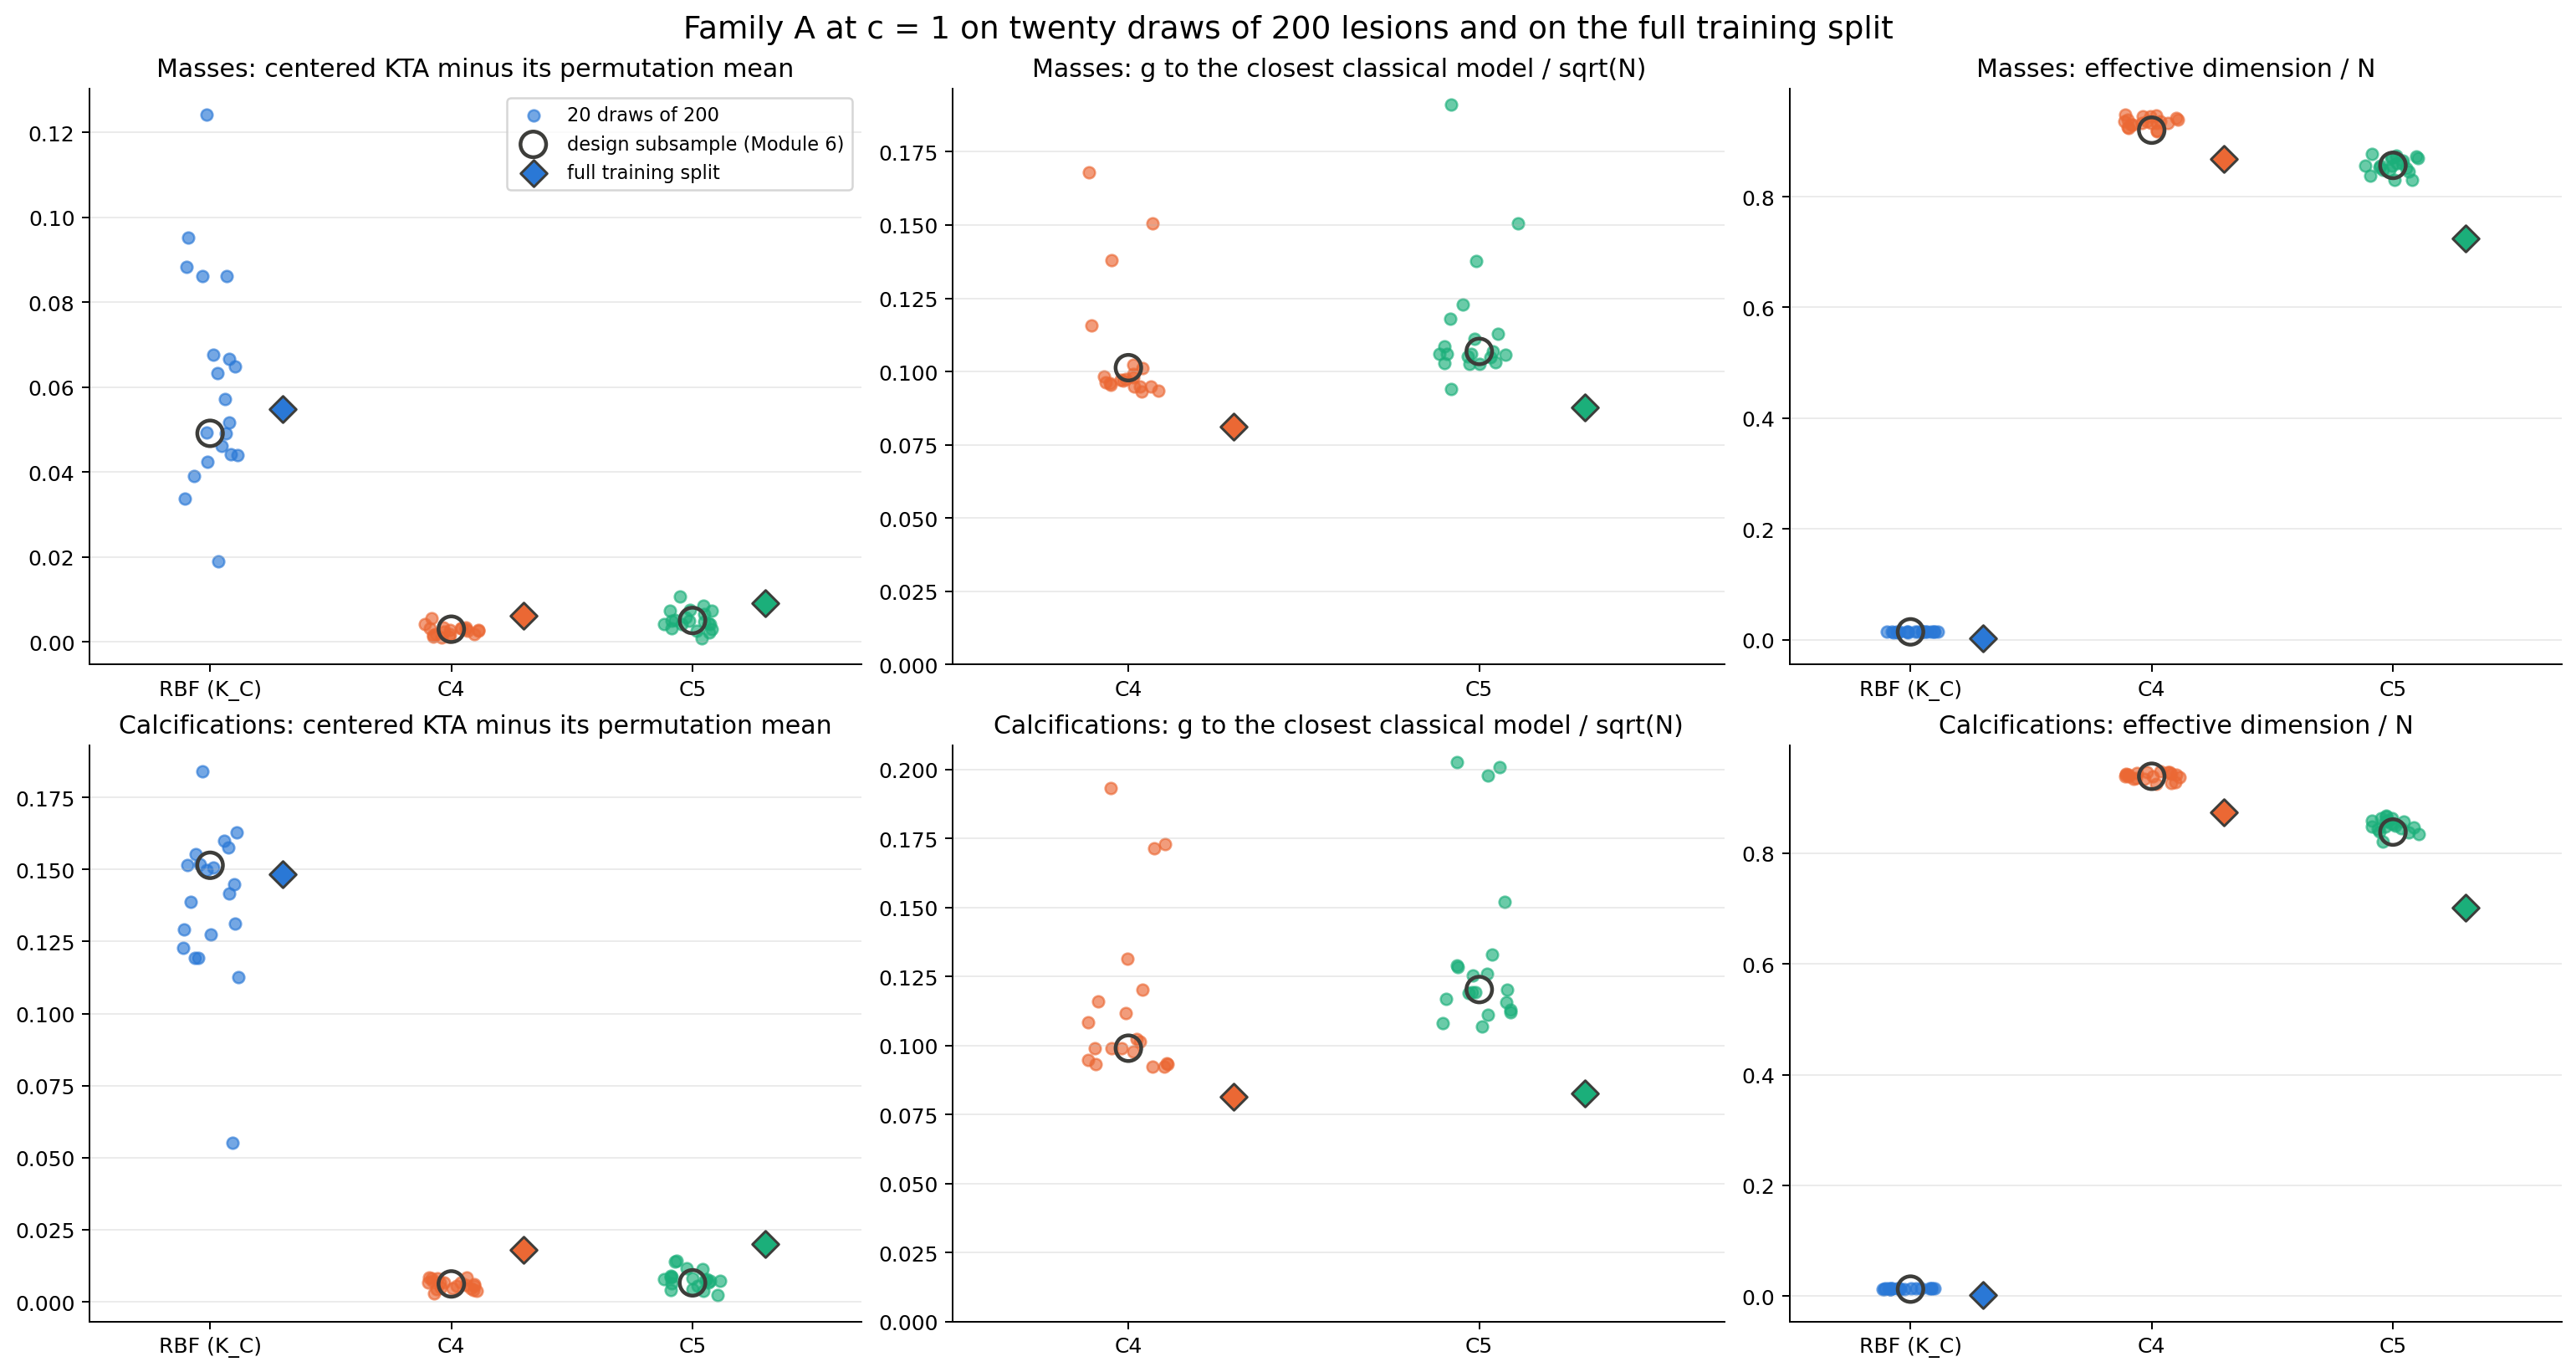
\includegraphics[width=\textwidth]{Figures/X9_sample_size.png}
% fuente: H-055; X9_familia_a.csv
\caption{Métricas de la familia de kernels a $c = 1$ en 20 submuestras de 200 lesiones (puntos), la submuestra del análisis principal (círculo) y todo el conjunto de entrenamiento (rombo).}
\label{fig:x9_sample_size}
\end{figure}

% fuente: H-036; X2_auc_pares.csv
En el análisis por pares sobre la submuestra de entrenamiento, el kernel clásico RBF obtuvo un
AUC de pares de 0.523 ($p = 0.002$) en masas y de 0.575 ($p = 0.001$) en calcificaciones. A escala $c = 1$,
C4 registró 0.510 ($p = 0.012$) en masas y 0.520 ($p = 0.021$) en calcificaciones, mientras que C5 obtuvo
0.508 ($p = 0.047$) en masas y 0.547 ($p = 0.001$) en calcificaciones. En calcificaciones, C5 superó a C4
en 0.027, aunque ambos kernels permanecieron por debajo del RBF. Al excluir los pares con fidelidad inferior
a $10^{-6}$, el AUC de pares de C5 se mantuvo en 0.510 en masas y 0.570 en calcificaciones, descartando que
la discriminación dependa de valores numéricamente irresolubles en hardware. La evolución del AUC de pares
se ilustra en la Figura~\ref{fig:x2_pair_auc_sweep}.

\begin{figure}[htbp]
\centering
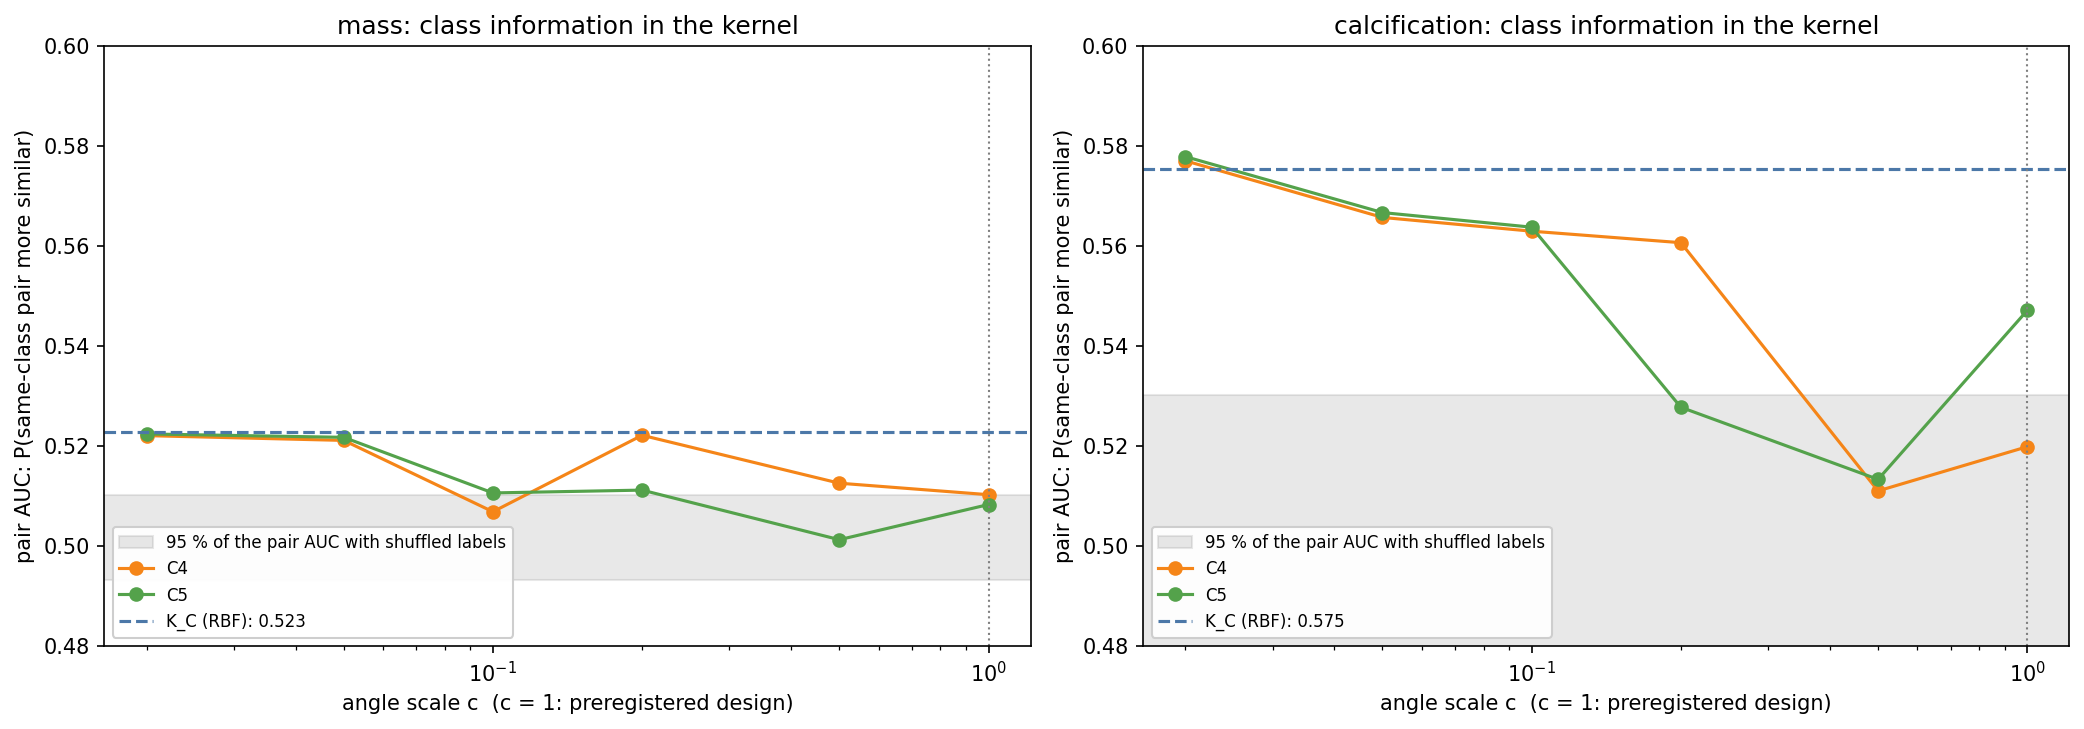
\includegraphics[width=\textwidth]{Figures/X2_pair_auc_sweep.png}
% fuente: H-036; X2_auc_pares.csv
\caption{Evolución del AUC de pares en función del factor de escala angular $c$ para kernels cuánticos y clásico.}
\label{fig:x2_pair_auc_sweep}
\end{figure}

% fuente: D-029, H-031, H-037, H-039; 8_oe6_shots_kernel.csv, 5b_concentracion_kernel.csv, 6_alineamiento_kernel.csv, 6_dimension_efectiva.csv, 6_diferencia_geometrica.csv
Al contraer los ángulos de rotación mediante el factor de escala $\mathbf{x} \to c\mathbf{x}$ con
$c \in \{1$, $0.5$, $0.2$, $0.1$, $0.05$, $0.02\}$, la concentración se reduce progresivamente: para $c = 0.02$,
la mediana fuera de la diagonal sube a 0.55 (C4) y 0.54 (C5) en masas, y a 0.59 y 0.58 en calcificaciones, el exceso de KTA alcanza
0.043 en masas y 0.143 en calcificaciones (próximo a 0.049 y 0.151 del RBF), la dimensión efectiva decae a
aproximadamente 4 y $g$ se ubica entre 2.1 y 2.5 (con un valor máximo de 3.1 en todo el barrido para C5 con $c = 0.5$).
Este incremento en alineamiento no representa información cuántica novedosa: la fase acumulada en el bloque $ZZ$
corresponde a $2\pi^2 - 2\pi c(x_i + x_j) + 2c^2 x_i x_j$, donde la fase constante es invariante y el producto
cruzado $x_i x_j$ decae con $c^2$. A escala $c = 0.02$, la correlación entre el kernel cuántico completo y una
versión idéntica que prescinde del producto entre características es de 0.99997 en masas y 0.99999 en calcificaciones.
La concentración del kernel solo se disipa cuando el término de interacción de segundo orden deja de tener efecto,
recuperando la estructura de similitud suave que un kernel clásico modela de forma directa.

% fuente: H-041; X3_comparacion_k8_k12.csv, X3_alineamiento_kernel.csv, X3_dimension_efectiva.csv, X3_diferencia_geometrica_resumen.csv
El experimento con un registro reducido a 8 qubits ($k = 8$) evaluó las ocho primeras características
de la selección con 28 bloques $ZZ$ y un circuito con 16 parámetros libres. Al reducir la dimensión, la concentración
disminuye: a $c = 1$, la mediana fuera de la diagonal asciende a 0.010 en C4 y 0.0015 en C5 para masas, y a 0.008 en C4
y 0.0008 en C5 para calcificaciones; la dimensión efectiva se reduce a 140 en C4 y 103 en C5 para masas, y a 170 en C4
y 131 en C5 para calcificaciones; y el exceso de KTA se incrementa entre 1.7 y 4.6 veces (0.012 en C4 y 0.023 en C5 para masas;
0.011 en C4 y 0.024 en C5 para calcificaciones), manteniéndose por debajo del RBF (0.049 y 0.150). La diferencia
geométrica mínima $g$ se ubicó en 2.40 en C4 y 3.23 en C5 para masas, y en 1.71 en C4 y 2.16 en C5 para calcificaciones,
muy por debajo de $\sqrt{N} = 14.1$. En las representaciones vectoriales sobre el entrenamiento completo, la condición
clásica C1 mantuvo la ventaja en la razón de Fisher: 0.37 frente a 0.09 (C4) y 0.17 (C5) en masas; y 0.98 frente a 0.29 (C4)
y 0.37 (C5) en calcificaciones. La síntesis comparativa se presenta en la Tabla~\ref{tab:comparacion_k8_k12} y la
Figura~\ref{fig:x3_kernel_metrics_k8_k12}.

% fuente: H-041; X3_comparacion_k8_k12.csv
\begin{table}[htbp]
\centering
\small
\caption{Comparación de métricas de separabilidad entre las configuraciones con $k = 12$ y $k = 8$ qubits ($c = 1$, submuestra de 200 lesiones por subconjunto).}
\label{tab:comparacion_k8_k12}
\begin{adjustbox}{max width=\linewidth}
\begin{tabular}{l r r r r}
\toprule
Métrica & Masas, $k = 12$ & Masas, $k = 8$ & Calcif., $k = 12$ & Calcif., $k = 8$ \\
\midrule
Mediana del kernel (C4 / C5) & 0.002 / 0.00003 & 0.010 / 0.0015 & 0.003 / 0.00003 & 0.008 / 0.0008 \\
Dimensión efectiva (C4 / C5 de 200) & 184.0 / 171.3 & 139.6 / 103.3 & 187.7 / 167.6 & 169.7 / 131.0 \\
Exceso de KTA (C4 / C5) & 0.003 / 0.005 & 0.012 / 0.023 & 0.006 / 0.007 & 0.011 / 0.024 \\
Exceso de KTA del RBF & 0.049 & 0.049 & 0.151 & 0.150 \\
$g$ mínima (C4 / C5; $\sqrt{N} \approx 14.1$) & 1.43 / 1.51 & 2.40 / 3.23 & 1.40 / 1.70 & 1.71 / 2.16 \\
Dispersión $\langle Z_i \rangle$ en todo el train (C4 / C5) & 0.058 / 0.180 & 0.099 / 0.276 & 0.048 / 0.178 & 0.076 / 0.267 \\
Fisher $J$ en todo el train (C1 / C4 / C5) & 0.45 / 0.13 / 0.21 & 0.37 / 0.09 / 0.17 & 1.06 / 0.42 / 0.31 & 0.98 / 0.29 / 0.37 \\
\bottomrule
\end{tabular}
\end{adjustbox}
\end{table}

\begin{figure}[htbp]
\centering
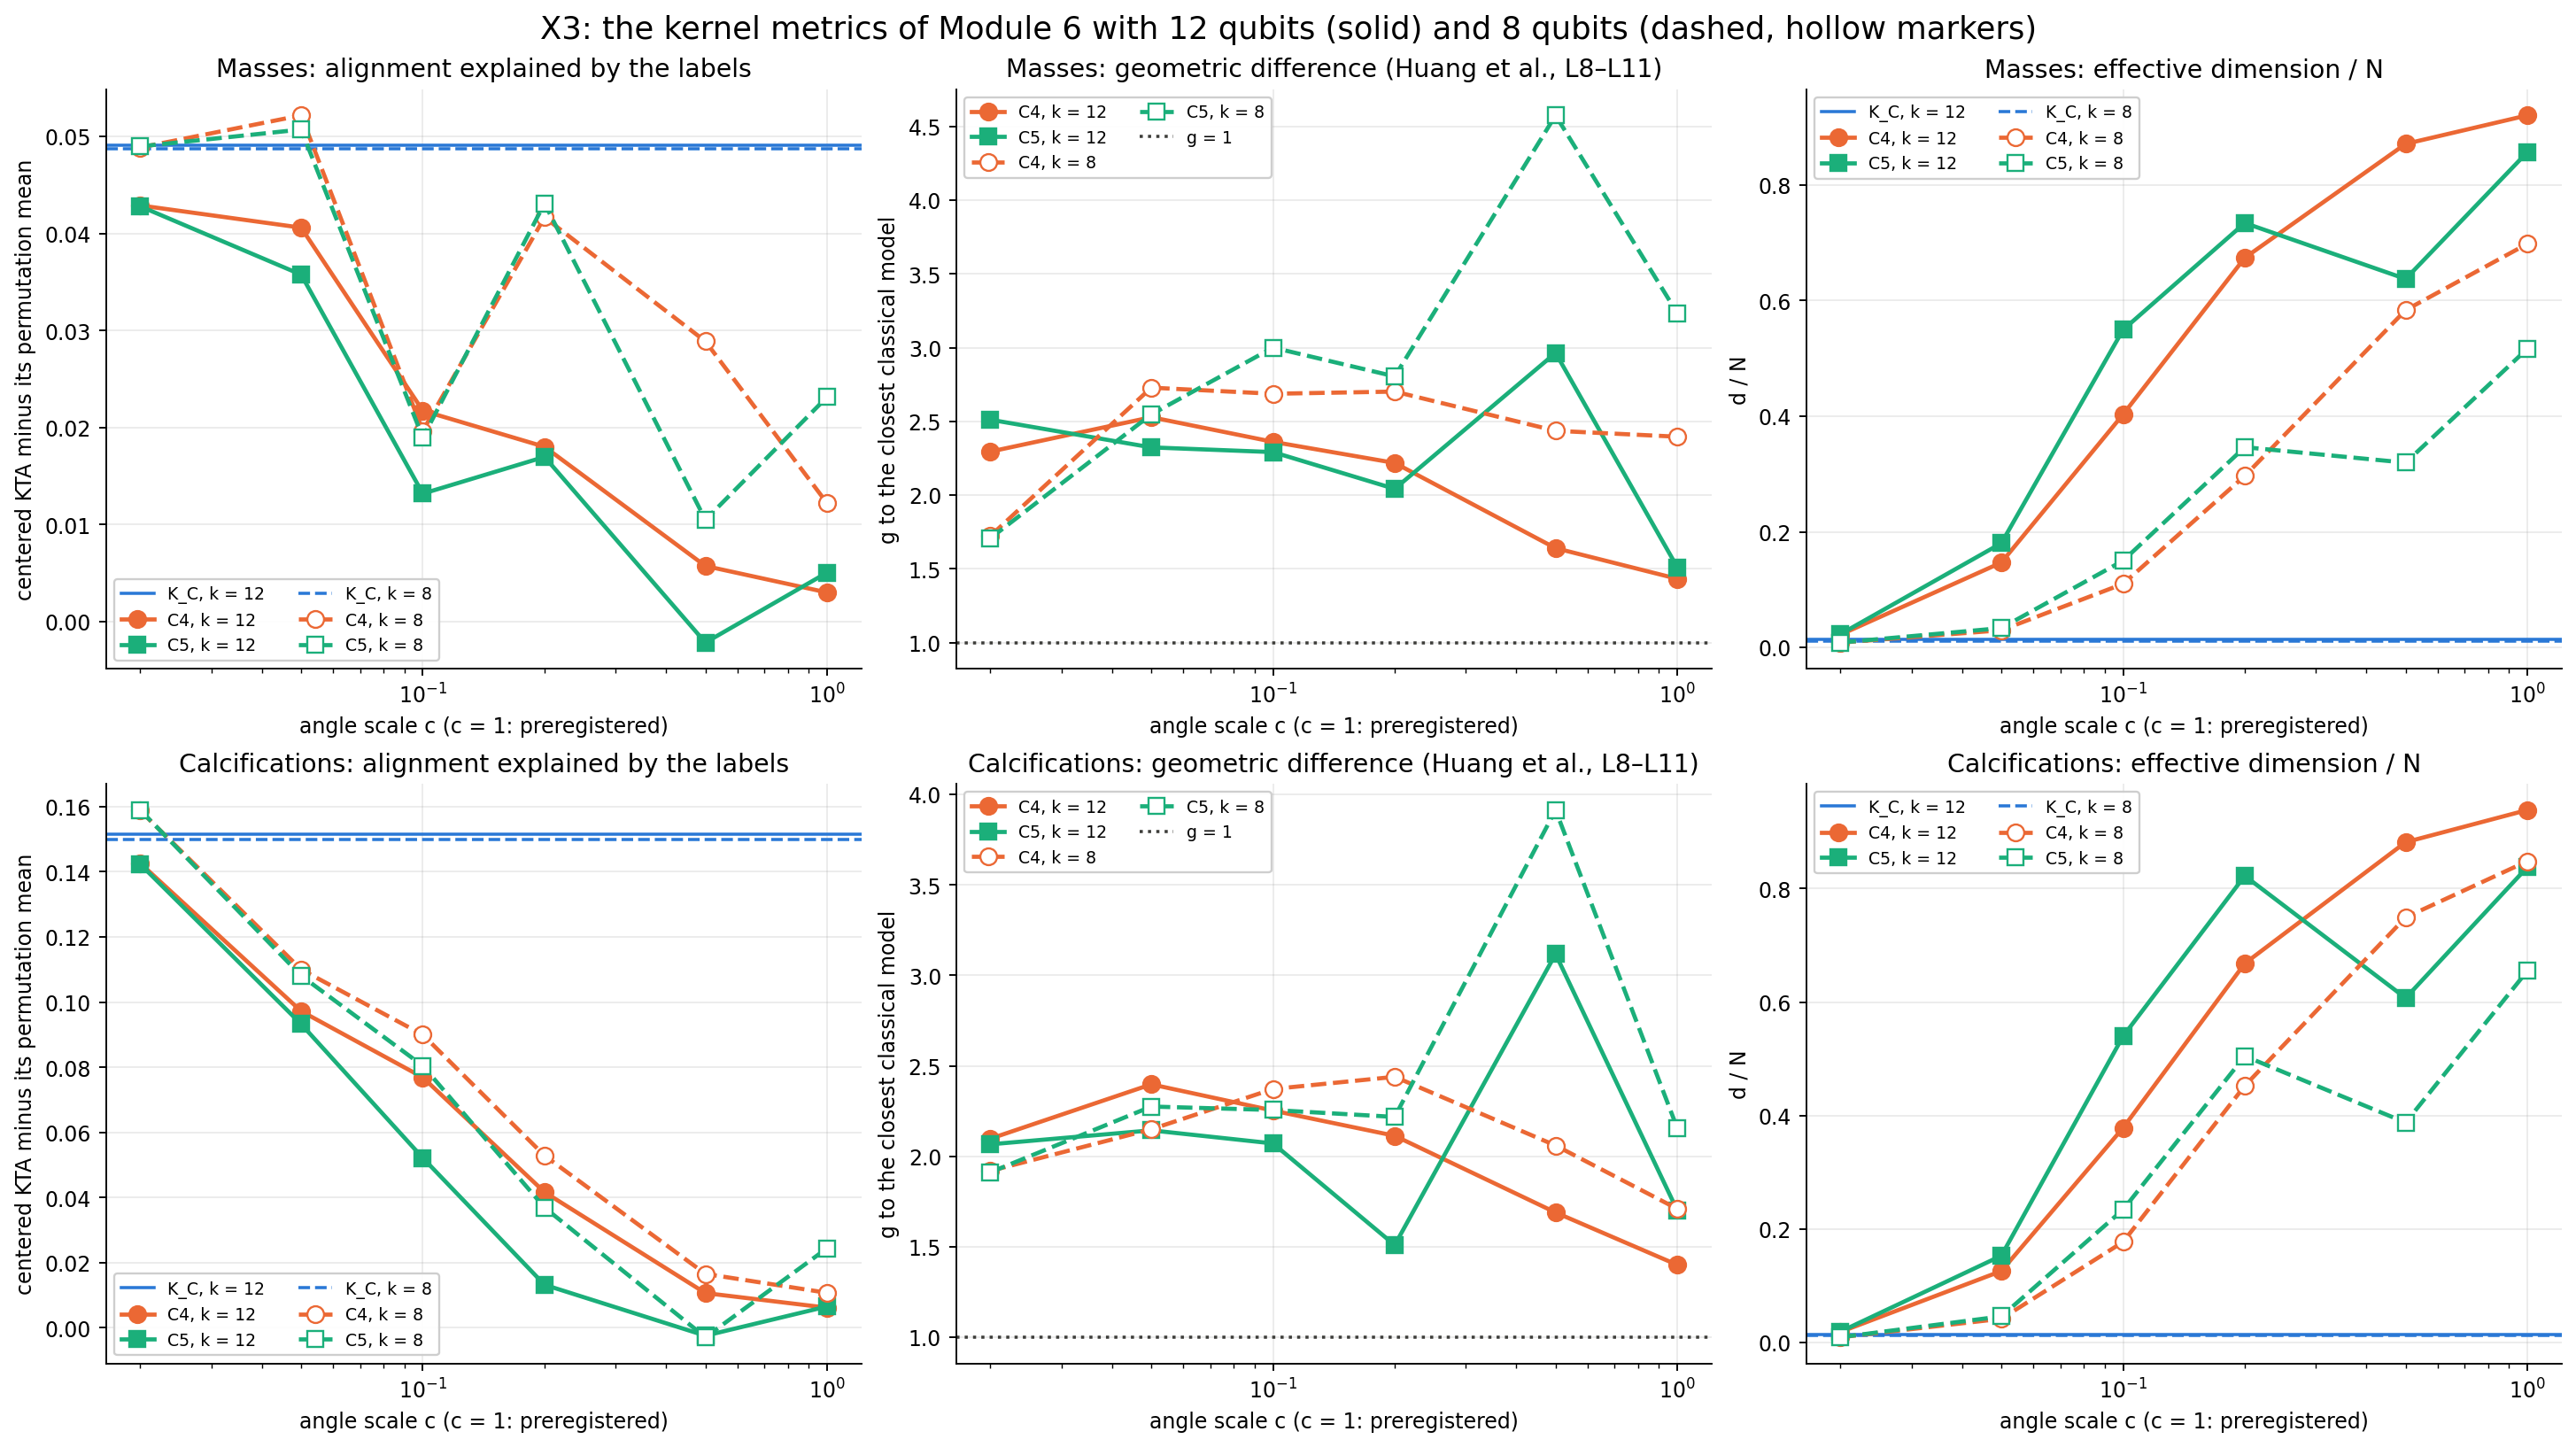
\includegraphics[width=\textwidth]{Figures/X3_kernel_metrics_k8_k12.png}
% fuente: H-041; X3_comparacion_k8_k12.csv
\caption{Comparación de métricas de separabilidad en kernels cuánticos entre configuraciones con 12 y 8 qubits.}
\label{fig:x3_kernel_metrics_k8_k12}
\end{figure}

% fuente: H-039
En conjunto, estos hallazgos proporcionan respuesta al objetivo específico OE-3: bajo la configuración
metodológica predefinida ($k = 12$, $c = 1$), las transformaciones cuánticas evaluadas no muestran una
separabilidad geométrica superior a la obtenida mediante representaciones y kernels clásicos, ni en la formulación
basada en fidelidades ni en la basada en valores esperados. Esta evidencia empírica describe la viabilidad y las
propiedades de separabilidad del espacio de estados cuánticos generado en el contexto del problema radiómico abordado.

% ---
% Reemplaza líneas 3458–3462 de Docs/Technical_Report.tex.
% Decisiones y hallazgos que lo respaldan: D-036, D-037, H-042, H-043, H-053, H-054.
% ---

\subsection{Clasificación}
\label{sec:rendimiento_clasificacion}

% fuente: H-042; 7_test.csv, 7_cv_resumen.csv
El protocolo de clasificación evalúa las cinco representaciones bajo una misma arquitectura de perceptrón multicapa ($k \to 32 \to 16 \to 1$) optimizada con entropía cruzada binaria ponderada. Los resultados sobre el conjunto de prueba oficial se detallan en el cuadro~\ref{tab:m7_clasificacion} y las diferencias pareadas correspondientes en el cuadro~\ref{tab:m7_diferencias}. En el subconjunto de masas, la condición de referencia C1 alcanza un AUC-ROC en el conjunto de prueba de 0.651 [IC 95\,\%: 0.578, 0.724] (0.652 $\pm$ 0.068 en validación cruzada), mientras que C2 obtiene 0.641 [0.572, 0.710] y C3 registra 0.646 [0.572, 0.721]. Las representaciones cuánticas obtienen un desempeño inferior: C4 alcanza un AUC de 0.530 [0.473, 0.587] (0.565 $\pm$ 0.079 en validación cruzada) y C5 logra 0.581 [0.521, 0.644] (0.563 $\pm$ 0.024 en validación cruzada). En masas, el clasificador sobre C4 no se distingue del azar en el conjunto de prueba.

% fuente: H-042; 7_test.csv, 7_cv_resumen.csv
En el subconjunto de calcificaciones, el desempeño general es más elevado en todas las condiciones. La condición C1 alcanza un AUC en el conjunto de prueba de 0.769 [0.694, 0.836] (0.742 $\pm$ 0.038 en validación cruzada), C2 obtiene 0.788 [0.719, 0.851] (0.758 $\pm$ 0.046 en validación cruzada) y C3 registra 0.758 [0.685, 0.826] (0.739 $\pm$ 0.036 en validación cruzada). Por su parte, las representaciones cuánticas descienden a 0.633 [0.558, 0.700] en C4 (0.640 $\pm$ 0.041 en validación cruzada) y a 0.652 [0.571, 0.725] en C5 (0.667 $\pm$ 0.035 en validación cruzada).

% fuente: H-042; 7_test_diferencias.csv
El comportamiento del control nulo resulta consistente con lo esperado: las diferencias pareadas entre C2 y C1 en el conjunto de prueba, de $-0.011$ [$-0.061$, $0.038$] ($p = 0.659$) en masas y de $0.020$ [$-0.026$, $0.067$] ($p = 0.377$) en calcificaciones, no resultan estadísticamente distinguibles de cero, como cabe esperar de una rotación, que no cambia la información disponible para el clasificador. En contraste, las representaciones cuánticas presentan pérdidas significativas respecto a C1: en masas, C4 $-$ C1 es de $-0.122$ [$-0.202$, $-0.044$] ($p = 0.003$) y C5 $-$ C1 es de $-0.070$ [$-0.140$, $-0.004$] ($p = 0.044$); en calcificaciones, C4 $-$ C1 es de $-0.135$ [$-0.208$, $-0.061$] ($p = 0.001$) y C5 $-$ C1 es de $-0.118$ [$-0.182$, $-0.046$] ($p < 0.001$). Frente a C3 las diferencias son comparables: en masas, $-0.116$ para C4 ($p = 0.006$) y $-0.065$ para C5 ($p = 0.058$); en calcificaciones, $-0.124$ para C4 ($p = 0.001$) y $-0.108$ para C5 ($p = 0.004$). La diferencia entre ambas condiciones cuánticas (C5 $-$ C4) no resulta estadísticamente significativa en ninguno de los subconjuntos: $0.051$ [$-0.027$, $0.128$] en masas y $0.017$ [$-0.061$, $0.098$] ($p = 0.679$) en calcificaciones.

% fuente: H-042; 7_test_diferencias.csv
Al considerar el problema de comparaciones múltiples sobre la familia de las cuatro diferencias cuánticas frente a C1 (C4 masas con $p \approx 0.003$, C4 calcificaciones con $p \approx 0.001$, C5 calcificaciones con $p < 0.001$ y C5 masas con $p \approx 0.044$), el procedimiento escalonado de Holm mantiene la significancia estadística de las cuatro diferencias a un nivel global $\alpha = 0.05$. Bajo la corrección más estricta de Bonferroni ($0.044 \times 4 \approx 0.18$), la diferencia de C5 en masas se sitúa en el límite y deja de ser estadísticamente significativa (figuras~\ref{fig:m7_auc} y~\ref{fig:m7_roc_test}).

\input{tablas/m7_clasificacion}

\input{tablas/m7_diferencias}

\begin{figure}[htbp]
\centering
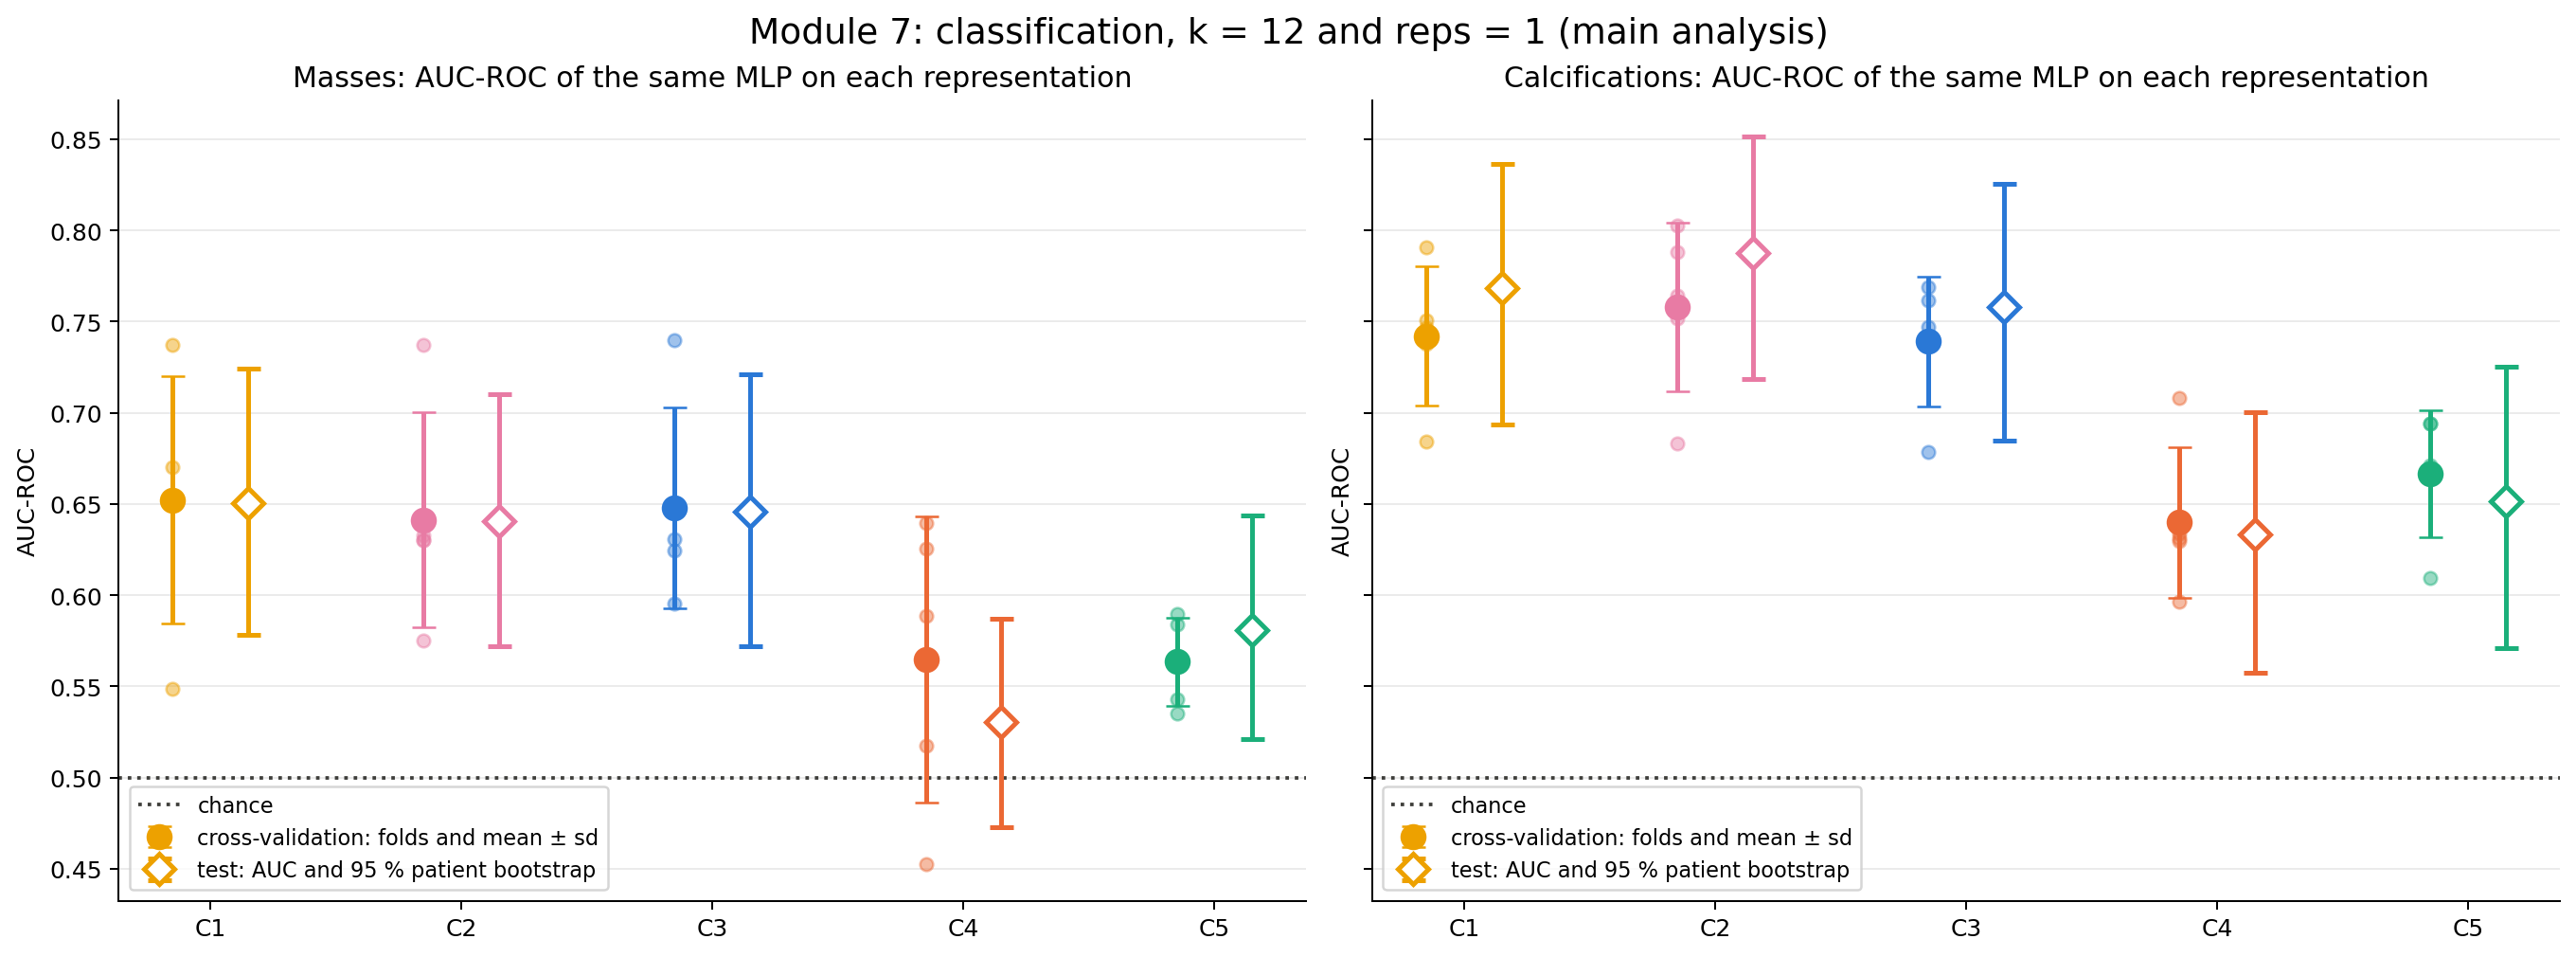
\includegraphics[width=\textwidth]{Figures/M7_auc.png}
\caption{Comparación de AUC-ROC entre las cinco condiciones evaluadas en validación cruzada y en el conjunto de prueba para masas y calcificaciones.}
\label{fig:m7_auc}
\end{figure}

\begin{figure}[htbp]
\centering
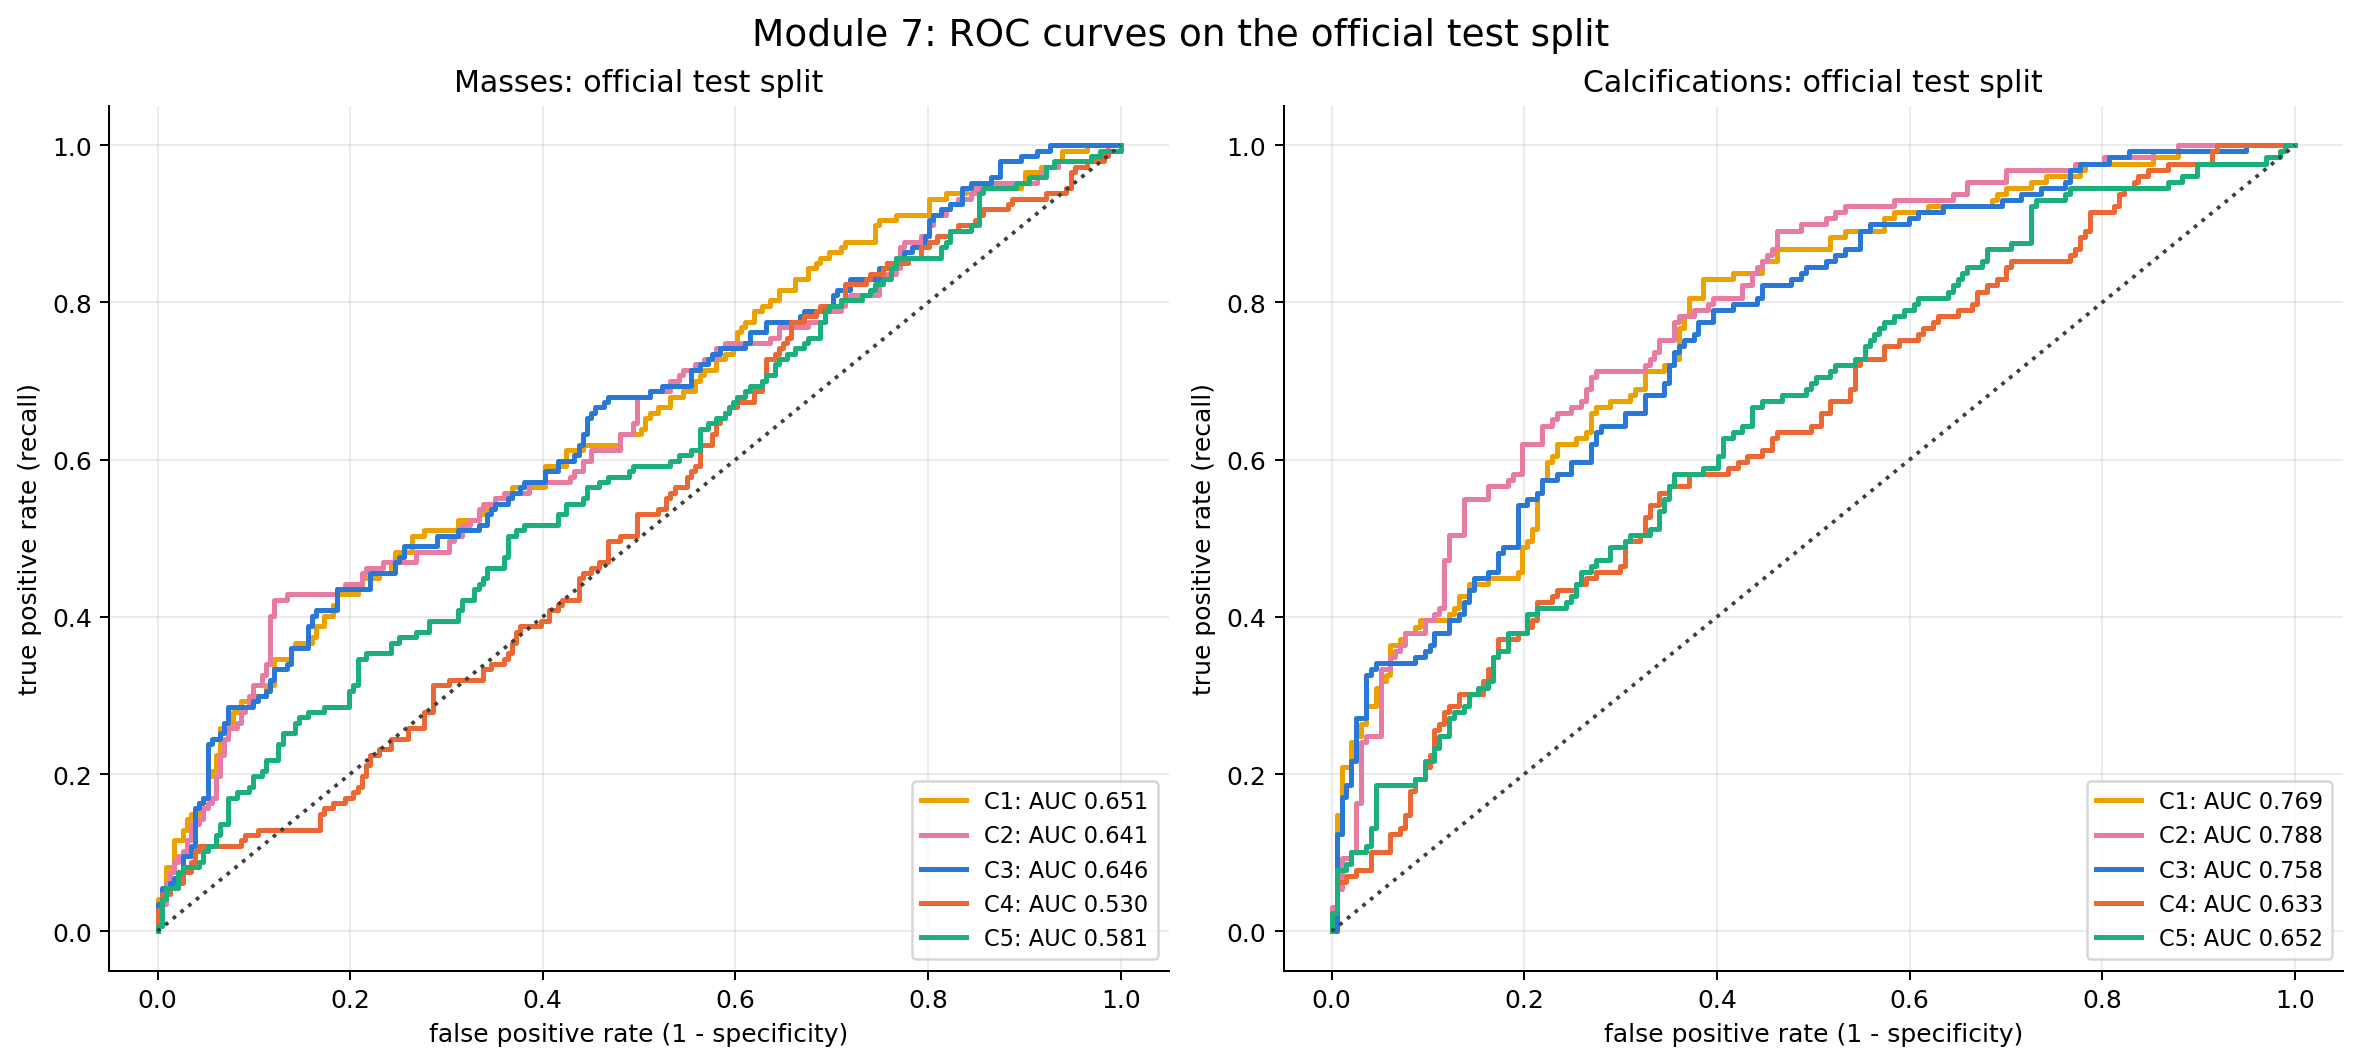
\includegraphics[width=\textwidth]{Figures/M7_roc_test.png}
\caption{Curvas ROC sobre el conjunto de prueba oficial para masas y calcificaciones bajo las cinco condiciones de representación.}
\label{fig:m7_roc_test}
\end{figure}

% fuente: H-043; 7_cv_resumen.csv, 7_test.csv, 7_test_diferencias.csv
El análisis de sensibilidad indica que la brecha observada entre condiciones clásicas y cuánticas se mantiene estable ante las variaciones evaluadas en la inicialización estocástica, la arquitectura de capas, la estandarización de las entradas y el régimen de épocas de entrenamiento. La dispersión del AUC medio en validación cruzada atribuible a la semilla del clasificador (semillas 42 a 46) no excede 0.039 en ninguna condición, lo que representa menos de la mitad de la brecha observada entre las condiciones clásicas y cuánticas (0.08 a 0.10). El empleo de arquitecturas alternativas de perceptrón multicapa (16-8 y 64-32) y el entrenamiento sin estandarización previa de entradas preservan exactamente el orden relativo de las condiciones. Por otra parte, forzar el entrenamiento a 200 épocas sin parada temprana no favorece a los modelos cuánticos: C4 y C5 deterioran su AUC medio a 0.533 y 0.557 en masas, y a 0.596 y 0.631 en calcificaciones, mientras que C1 se mantiene o mejora (0.680 en masas). Los modelos sobre representaciones cuánticas detienen su entrenamiento temprano debido a que la pérdida en el conjunto de validación cesa de mejorar, y no por subentrenamiento.

% fuente: H-043; 7_test.csv, 7_test_diferencias.csv
Al profundizar el \textit{ansatz} a dos repeticiones (\texttt{reps} = 2), la dispersión en datos reales con el vector de parámetros $\boldsymbol\theta$ fijado disminuye en C4 (de 0.058 a 0.047 en masas) y se incrementa en C5 (de 0.180 a 0.196). En clasificación, C5 mejora en el conjunto de prueba (de 0.581 a 0.603 en masas y de 0.652 a 0.682 en calcificaciones), si bien sus intervalos de diferencia frente a C1 se mantienen negativos: $-0.048$ [$-0.093$, $-0.005$] en masas y $-0.086$ [$-0.141$, $-0.034$] en calcificaciones. La condición C4 no presenta cambios apreciables. Finalmente, al reducir la dimensionalidad a $k = 8$ qubits, las condiciones clásicas prácticamente no varían, mientras que C4 tiende a empeorar en calcificaciones, alcanzando 0.561 en el conjunto de prueba con una diferencia de $-0.070$ [$-0.141$, $+0.0005$] respecto a $k = 12$, cuyo intervalo llega al cero. En este régimen de $k = 8$, las condiciones cuánticas se ubican entre 0.07 y 0.19 por debajo de C1 en el conjunto de prueba, lo cual es consistente con la observación de que una mayor dispersión geométrica en el espacio de expectativas no garantiza una mejora en la capacidad de discriminación del clasificador supervisado (figura~\ref{fig:m7_sensitivity}).

\begin{figure}[htbp]
\centering
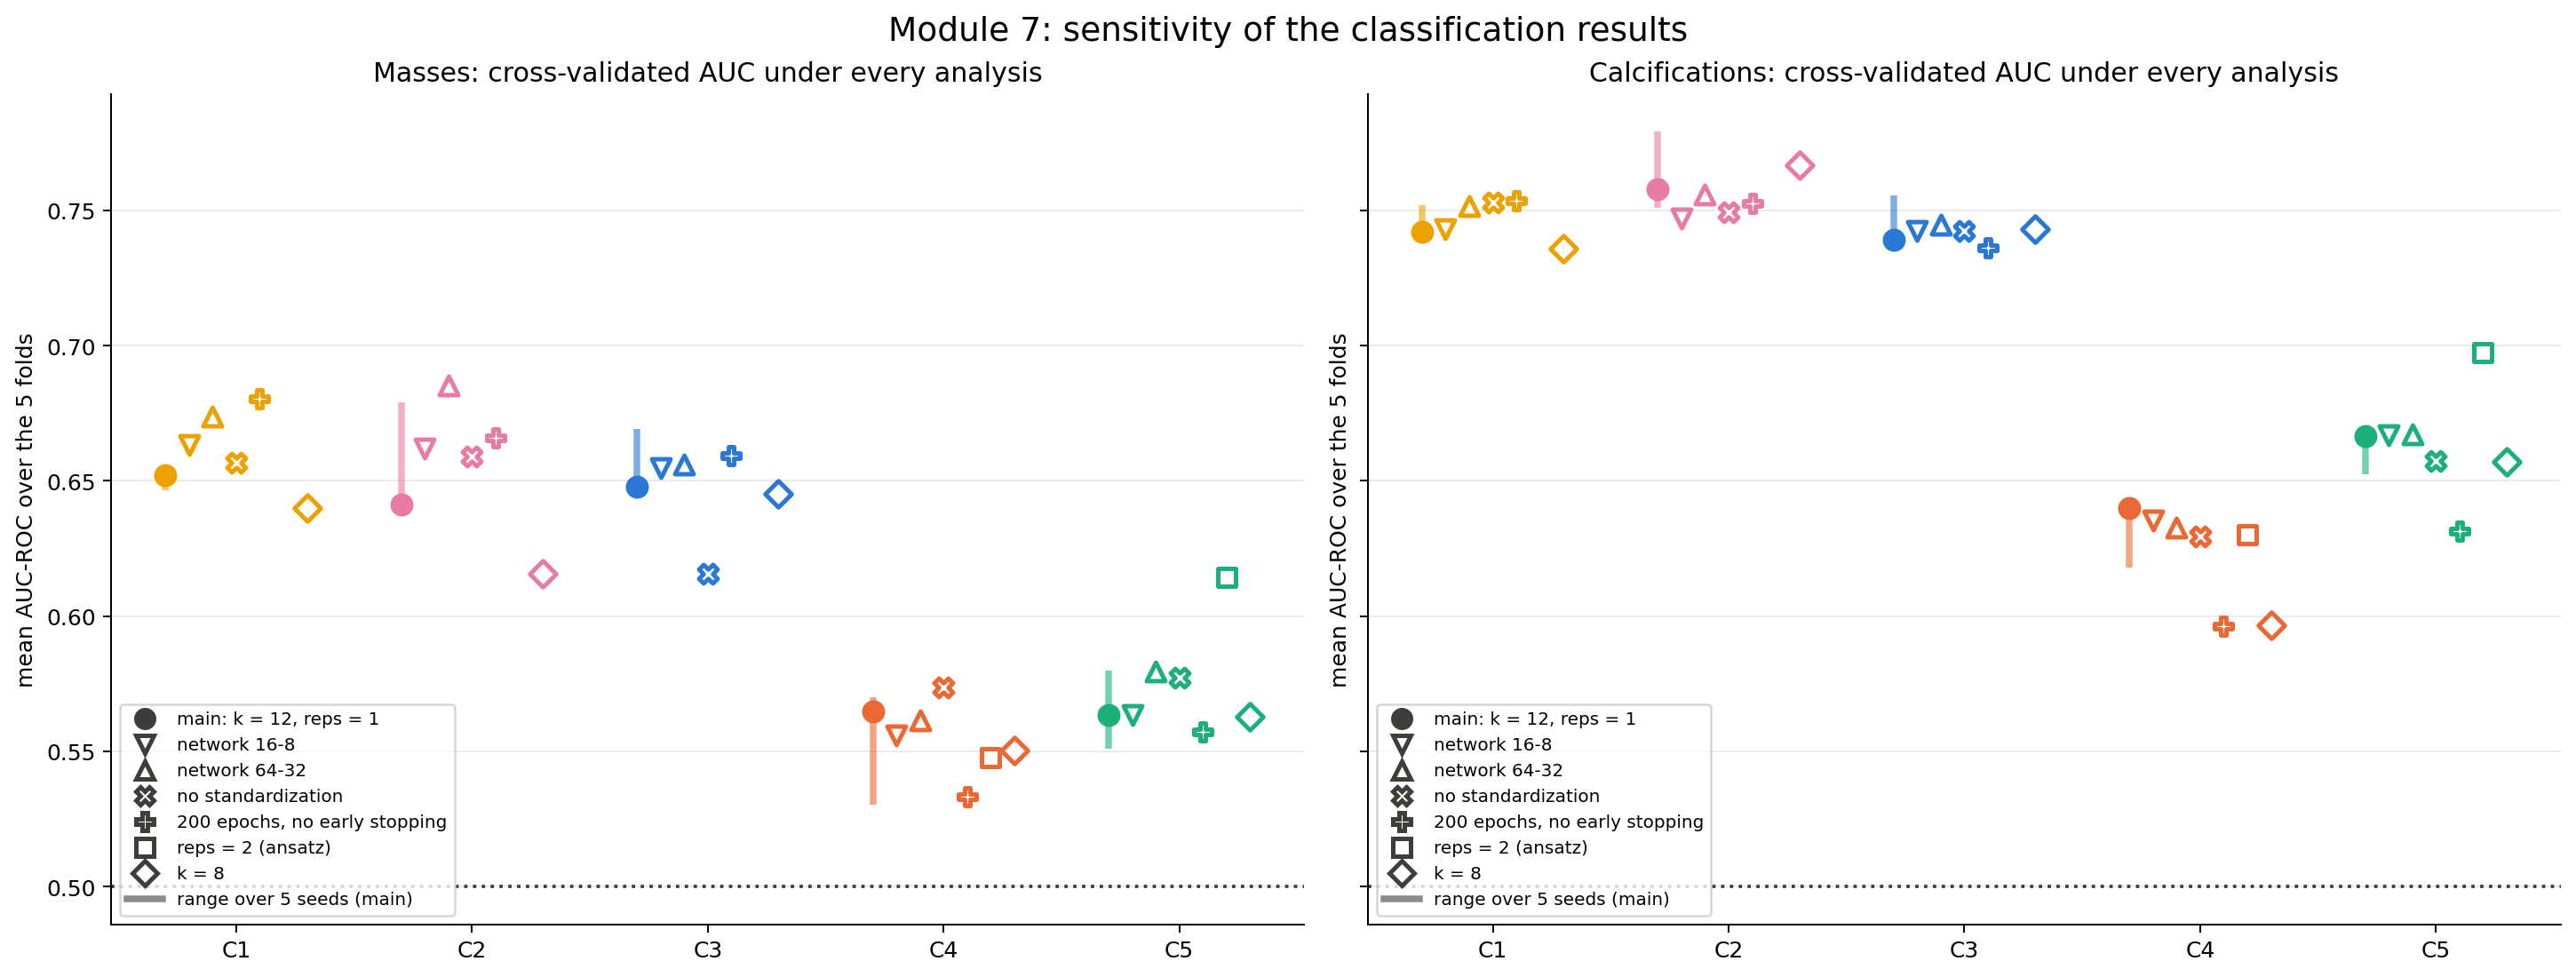
\includegraphics[width=\textwidth]{Figures/M7_sensitivity.png}
\caption{Análisis de sensibilidad del rendimiento de clasificación frente a cambios de semilla, arquitectura de red, escalado, épocas fijas, profundidad de circuito (\texttt{reps} = 2) y dimensión de entrada ($k = 8$).}
\label{fig:m7_sensitivity}
\end{figure}

% fuente: H-053; X7_resumen.csv, X7_sorteos.csv
\input{tablas/x7_sorteos_theta}

% fuente: H-053; X7_resumen.csv, X7_sorteos.csv
La evaluación de diez sorteos aleatorios independientes del vector de parámetros $\boldsymbol\theta$ (semillas 42 a 51) sobre los mismos pliegues de validación cruzada revela que $\boldsymbol\theta$ constituye una fuente de variación relevante, como se expone en el cuadro~\ref{tab:x7_theta}. El rango de variación del AUC debido a la elección de $\boldsymbol\theta$ oscila entre 0.040 y 0.110 (0.042 en C4 masas, 0.068 en C5 masas, 0.110 en C4 calcificaciones y 0.040 en C5 calcificaciones), igualando o superando la variación inducida por la semilla del clasificador (0.018 a 0.039). La semilla 42 establecida en el diseño inicial no constituye un caso sesgado: ocupa la sexta posición en C4 para ambos subconjuntos, la novena en C5 masas y la primera en C5 calcificaciones. Fundamentalmente, ninguno de los 40 sorteos evaluados alcanza el AUC de C1 (0.652 en masas y 0.742 en calcificaciones) ni de C3: el mejor sorteo queda entre 0.028 y 0.075 por debajo de C1, y el déficit frente a C1 se sitúa entre 0.03 y 0.18 según el sorteo. Asimismo, la correlación de Spearman entre la dispersión de $\langle Z_i \rangle$ y el AUC entre sorteos resulta no significativa en todos los casos ($p > 0.29$: 0.09 y $-0.02$ en masas; 0.03 y $-0.37$ en calcificaciones). Cabe destacar que los productos internos y las matrices de kernel no dependen de $\boldsymbol\theta$, dado que el operador unitario $V(\boldsymbol\theta)$ se cancela en el cálculo de fidelidades ($V(\boldsymbol\theta)^\dagger V(\boldsymbol\theta) = I$) (figura~\ref{fig:x7_theta_draws}).

\begin{figure}[htbp]
\centering
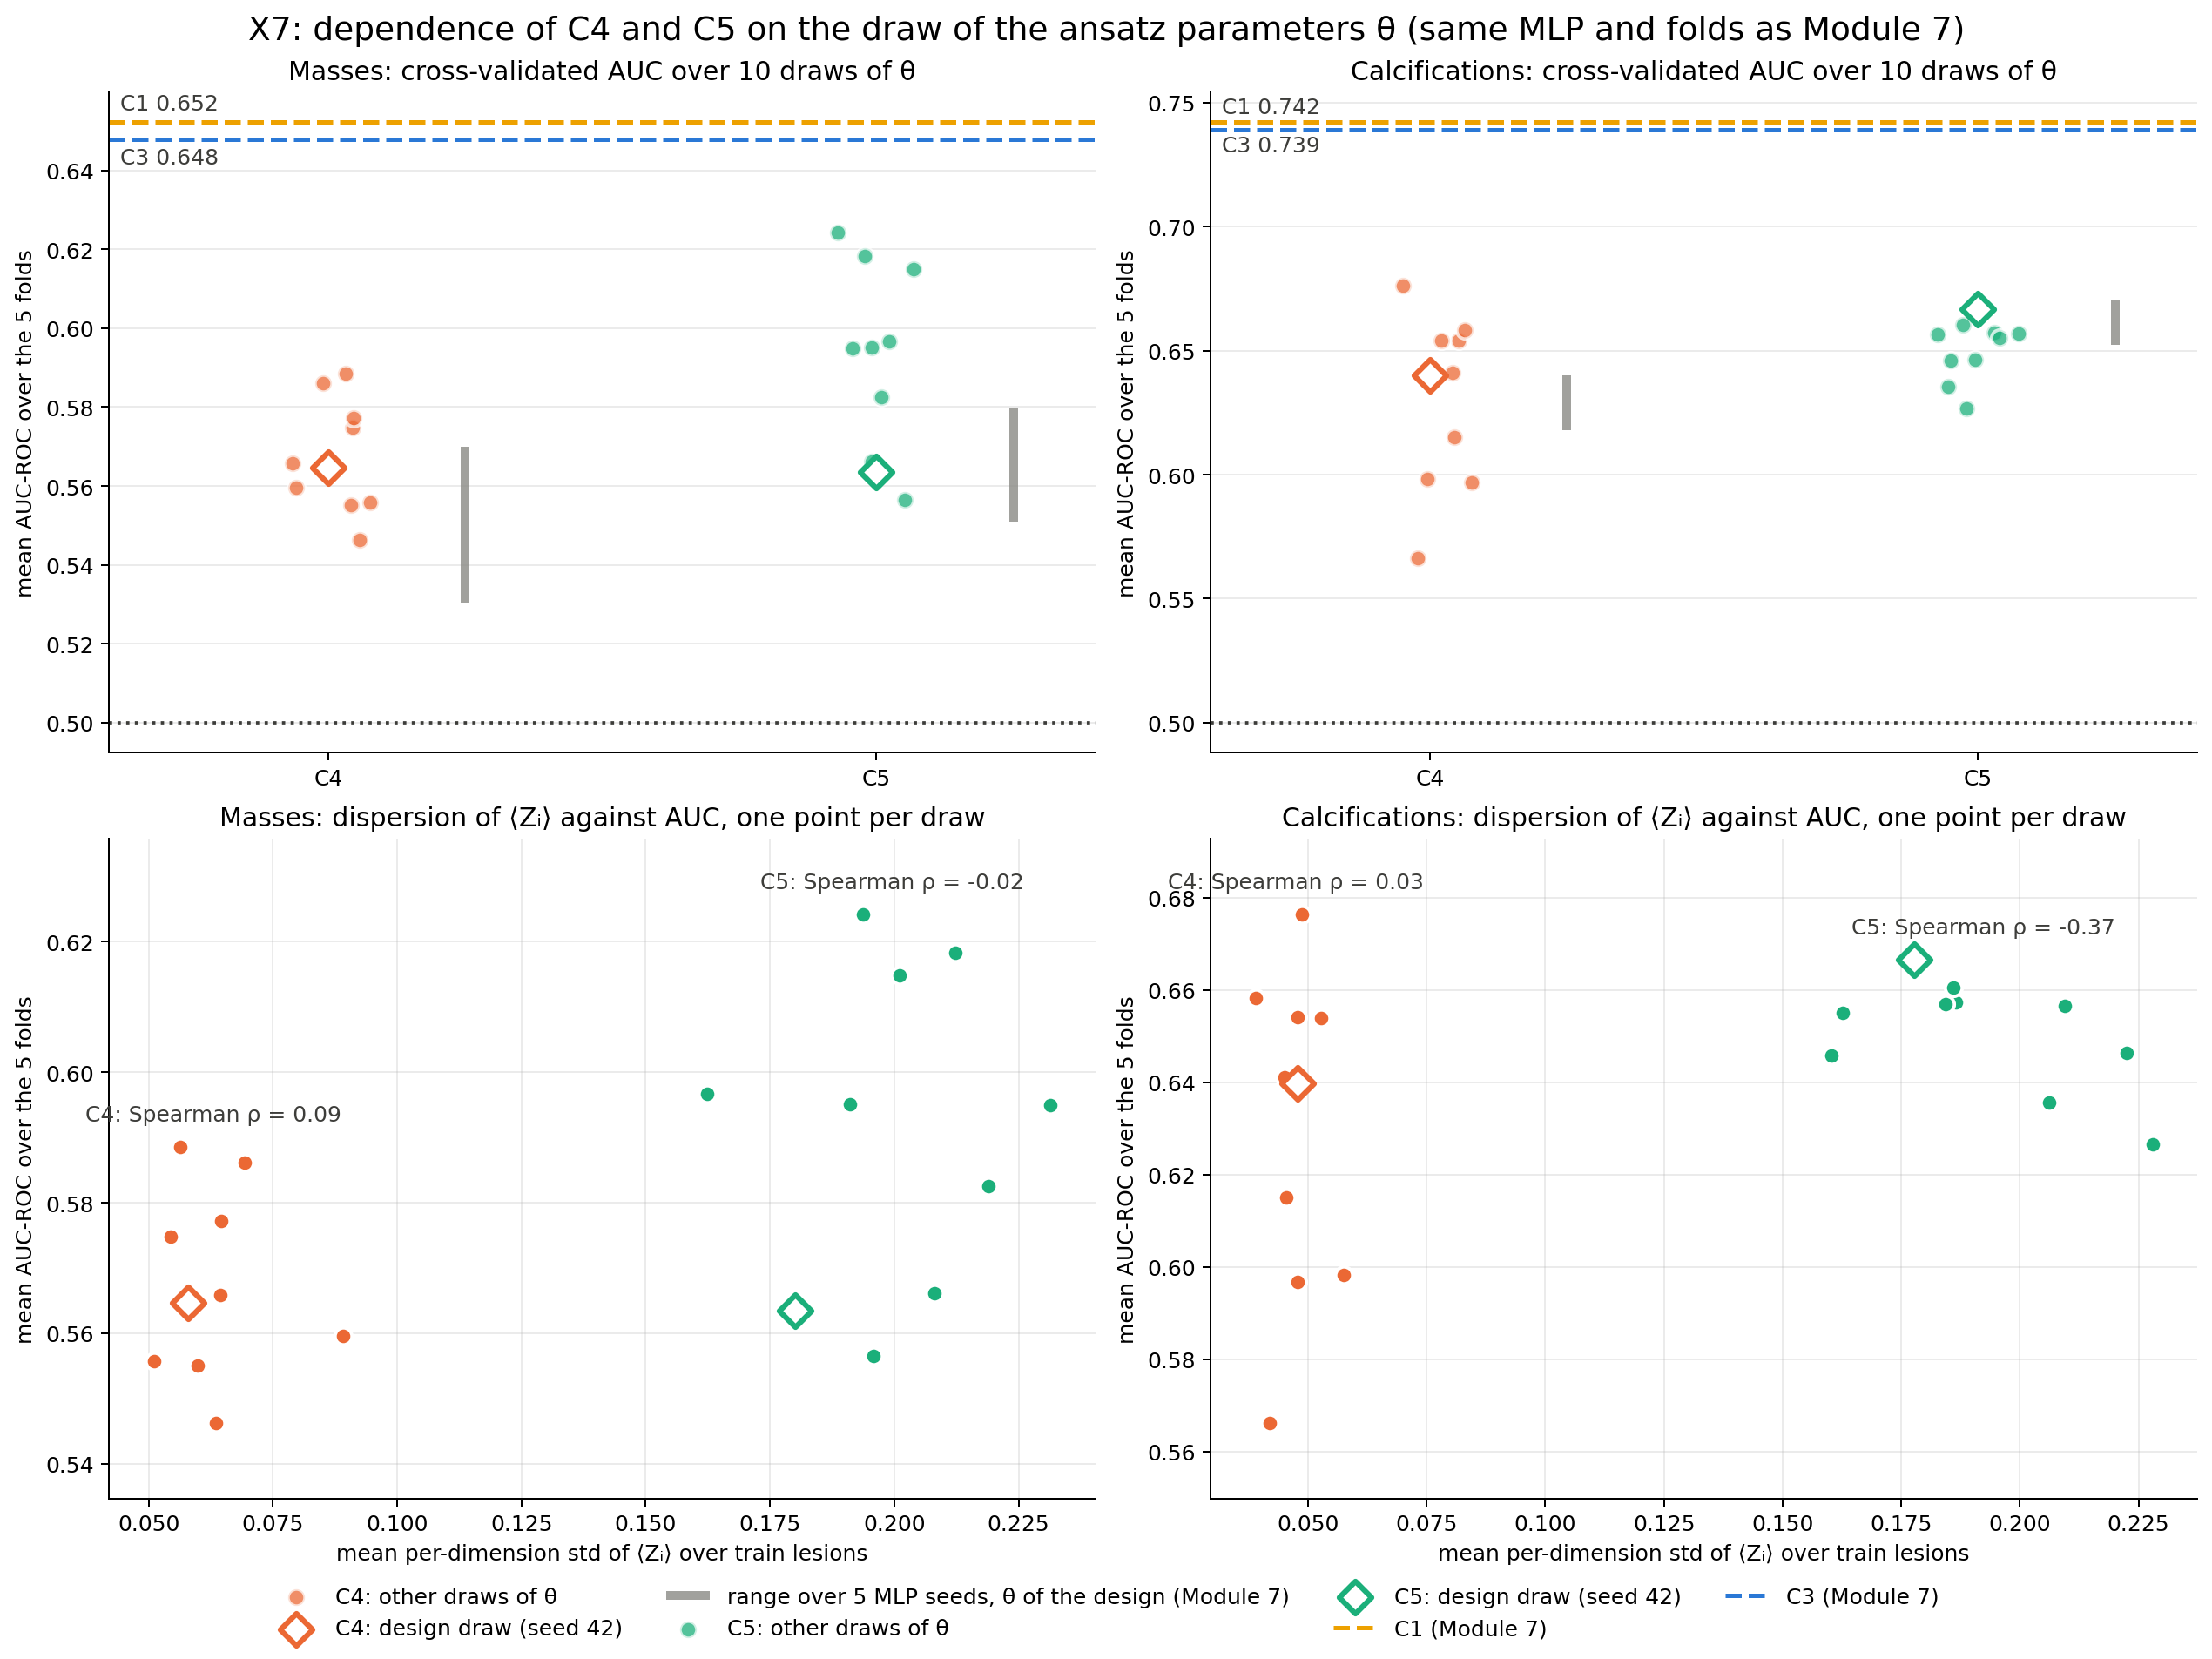
\includegraphics[width=\textwidth]{Figures/X7_theta_draws.png}
\caption{Distribución del AUC en validación cruzada a lo largo de diez sorteos aleatorios independientes de $\boldsymbol\theta$ para C4 y C5 en masas y calcificaciones.}
\label{fig:x7_theta_draws}
\end{figure}

% fuente: H-054; X8_test.csv, X8_test_diferencias.csv, X8_theta_entrenado.csv
\input{tablas/x8_theta_entrenado}

% fuente: H-054; X8_test.csv, X8_test_diferencias.csv, X8_costo_gradiente.csv
El entrenamiento conjunto de los parámetros $\boldsymbol\theta$ junto con los pesos del clasificador, partiendo del sorteo inicial de diseño, produce únicamente ganancias marginales que no resultan estadísticamente significativas, según se muestra en el cuadro~\ref{tab:x8_theta}. En el conjunto de prueba, la ganancia en AUC respecto a $\boldsymbol\theta$ fijo es de $+0.003$ [$-0.06$, $0.07$] en C4 masas (0.530 a 0.533), $+0.004$ [$-0.05$, $0.06$] en C5 masas (0.581 a 0.585), $+0.041$ [$-0.03$, $0.10$] en C4 calcificaciones (0.633 a 0.674) y $+0.020$ [$-0.04$, $0.08$] en C5 calcificaciones (0.652 a 0.671), abarcando en todos los casos el cero. Las cuatro combinaciones continúan ubicándose por debajo de C1 en el conjunto de prueba, con intervalos que excluyen el cero (diferencias de $-0.118$, $-0.066$, $-0.094$ y $-0.098$). Los parámetros $\boldsymbol\theta$ experimentan desplazamientos medios reducidos (0.13 a 0.39 radianes) y la época óptima de validación se alcanza entre la 4 y la 27, indicando que los 24 parámetros adicionales aportan sobreajuste antes que capacidad discriminativa generalizable.

% fuente: H-054; X8_costo_gradiente.csv
En términos de viabilidad computacional, la obtención del gradiente exacto mediante la regla de \textit{parameter-shift} (el procedimiento exigido en procesadores cuánticos físicos, con evaluaciones en $\pm \pi/2$) demanda 48 ejecuciones de circuito por lesión (5.2\,s por muestra a $k = 12$). Esto proyecta un coste de aproximadamente 205 horas de simulación por mapa de características para 50 épocas sobre el conjunto de entrenamiento. En contraste, la diferenciación automática por retropropagación analítica sobre el vector de estado en el simulador ejecuta cada muestra en 1.4\,ms (~3\,600 veces más rápido, completando 50 épocas en ~3.4 minutos) y reproduce el Jacobiano con una discrepancia numérica de apenas $1.8 \times 10^{-15}$. No obstante, este atajo analítico solo es posible en simulación clásica mediante el acceso a las 4\,096 amplitudes complejas del estado, y no existe en un computador cuántico real debido al colapso del estado inducido por la medición (figura~\ref{fig:x8_trained_theta}).

\begin{figure}[htbp]
\centering
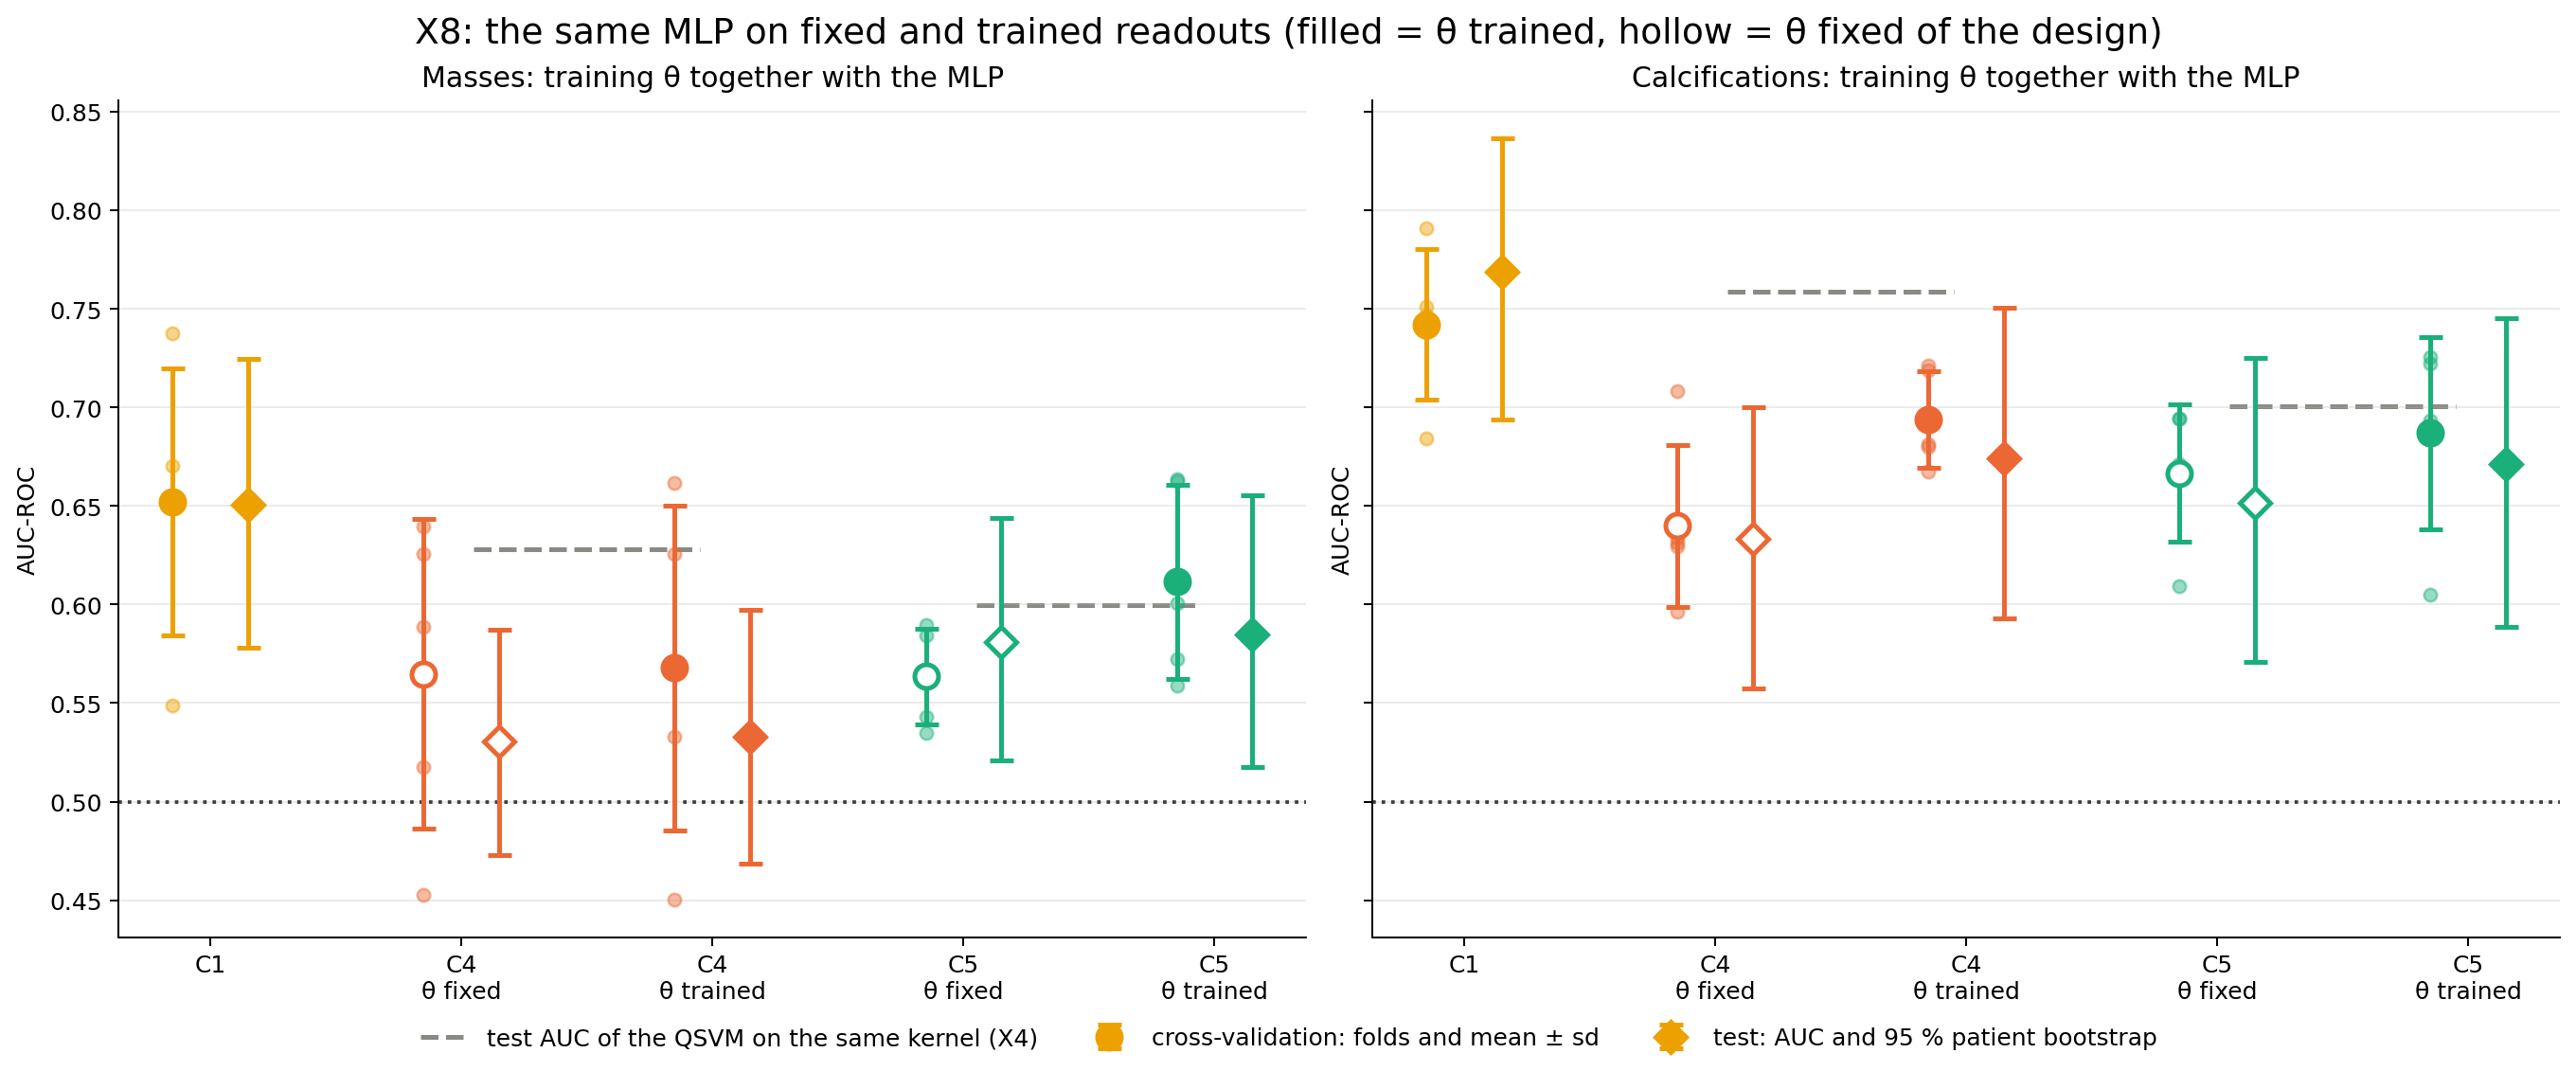
\includegraphics[width=\textwidth]{Figures/X8_trained_theta.png}
\caption{Desempeño de clasificación al entrenar los parámetros variacionales $\boldsymbol\theta$ junto con la red neuronal en comparación con $\boldsymbol\theta$ fijo, la referencia clásica C1 y el clasificador de kernel cuántico.}
\label{fig:x8_trained_theta}
\end{figure}

% ---
% Reemplaza líneas 3458–3462 de Docs/Technical_Report.tex.
% Decisiones y hallazgos que lo respaldan: D-038, H-044, H-045, H-046, H-047, H-048.
% ---

\subsection{Clasificadores de kernel y búsqueda de ventaja}

% fuente: H-044; X4_test.csv, X4_test_diferencias.csv
Para dilucidar si el rendimiento inferior observado en el perceptrón multicapa obedece a la codificación cuántica de los datos o al método de lectura, se evaluó un clasificador de vectores de soporte con kernel cuántico (QSVM) con regularización $C = 1$ y escala fija $c = 1$. En el conjunto de prueba oficial, el SVM clásico con kernel de base radial (RBF) alcanza un AUC-ROC de 0.649 [IC 95\,\%: 0.57, 0.73] en masas y de 0.769 [0.70, 0.83] en calcificaciones. El QSVM evaluado sobre el kernel cuántico de la condición C4 obtiene 0.628 [0.55, 0.70] en masas y 0.759 [0.69, 0.83] en calcificaciones, mientras que con el kernel de C5 logra 0.599 [0.52, 0.68] y 0.701 [0.62, 0.78]. La diferencia pareada entre el QSVM sobre C4 y el SVM RBF clásico resulta estadísticamente indistinguible de cero: $-0.02$ [$-0.05$, $0.01$] en masas y $-0.01$ [$-0.04$, $0.02$] en calcificaciones.

% fuente: H-044; X4_test.csv, X4_test_diferencias.csv
En contraste, al comparar el QSVM sobre el kernel de C4 frente al clasificador entrenado sobre las expectativas locales $\langle Z_i \rangle$ de C4 (AUC de 0.530 [0.47, 0.59] en masas y 0.633 [0.56, 0.70] en calcificaciones), el QSVM supera al modelo sobre expectativas en $+0.10$ [$0.03$, $0.17$] en masas y en $+0.13$ [$0.05$, $0.20$] en calcificaciones. Esta evidencia demuestra que la codificación cuántica en el espacio de Hilbert preserva prácticamente la totalidad de la información diagnóstica; la degradación ocurre en la etapa de lectura al proyectar un estado de 4\,096 amplitudes complejas en solo 12 valores esperados locales tras un circuito variacional fijo. Al optimizar la escala angular $c$ por validación cruzada, el QSVM con C4 iguala al mejor kernel clásico en el conjunto de prueba (diferencias de $-0.002$ en masas con $c = 0.05$ y $-0.005$ en calcificaciones con $c = 0.2$), en concordancia con el valor moderado de la diferencia geométrica ($g \approx 1.4 \ll \sqrt{N}$) formulada por Huang et al. \cite{huang2021power}.

\begin{figure}[htbp]
\centering
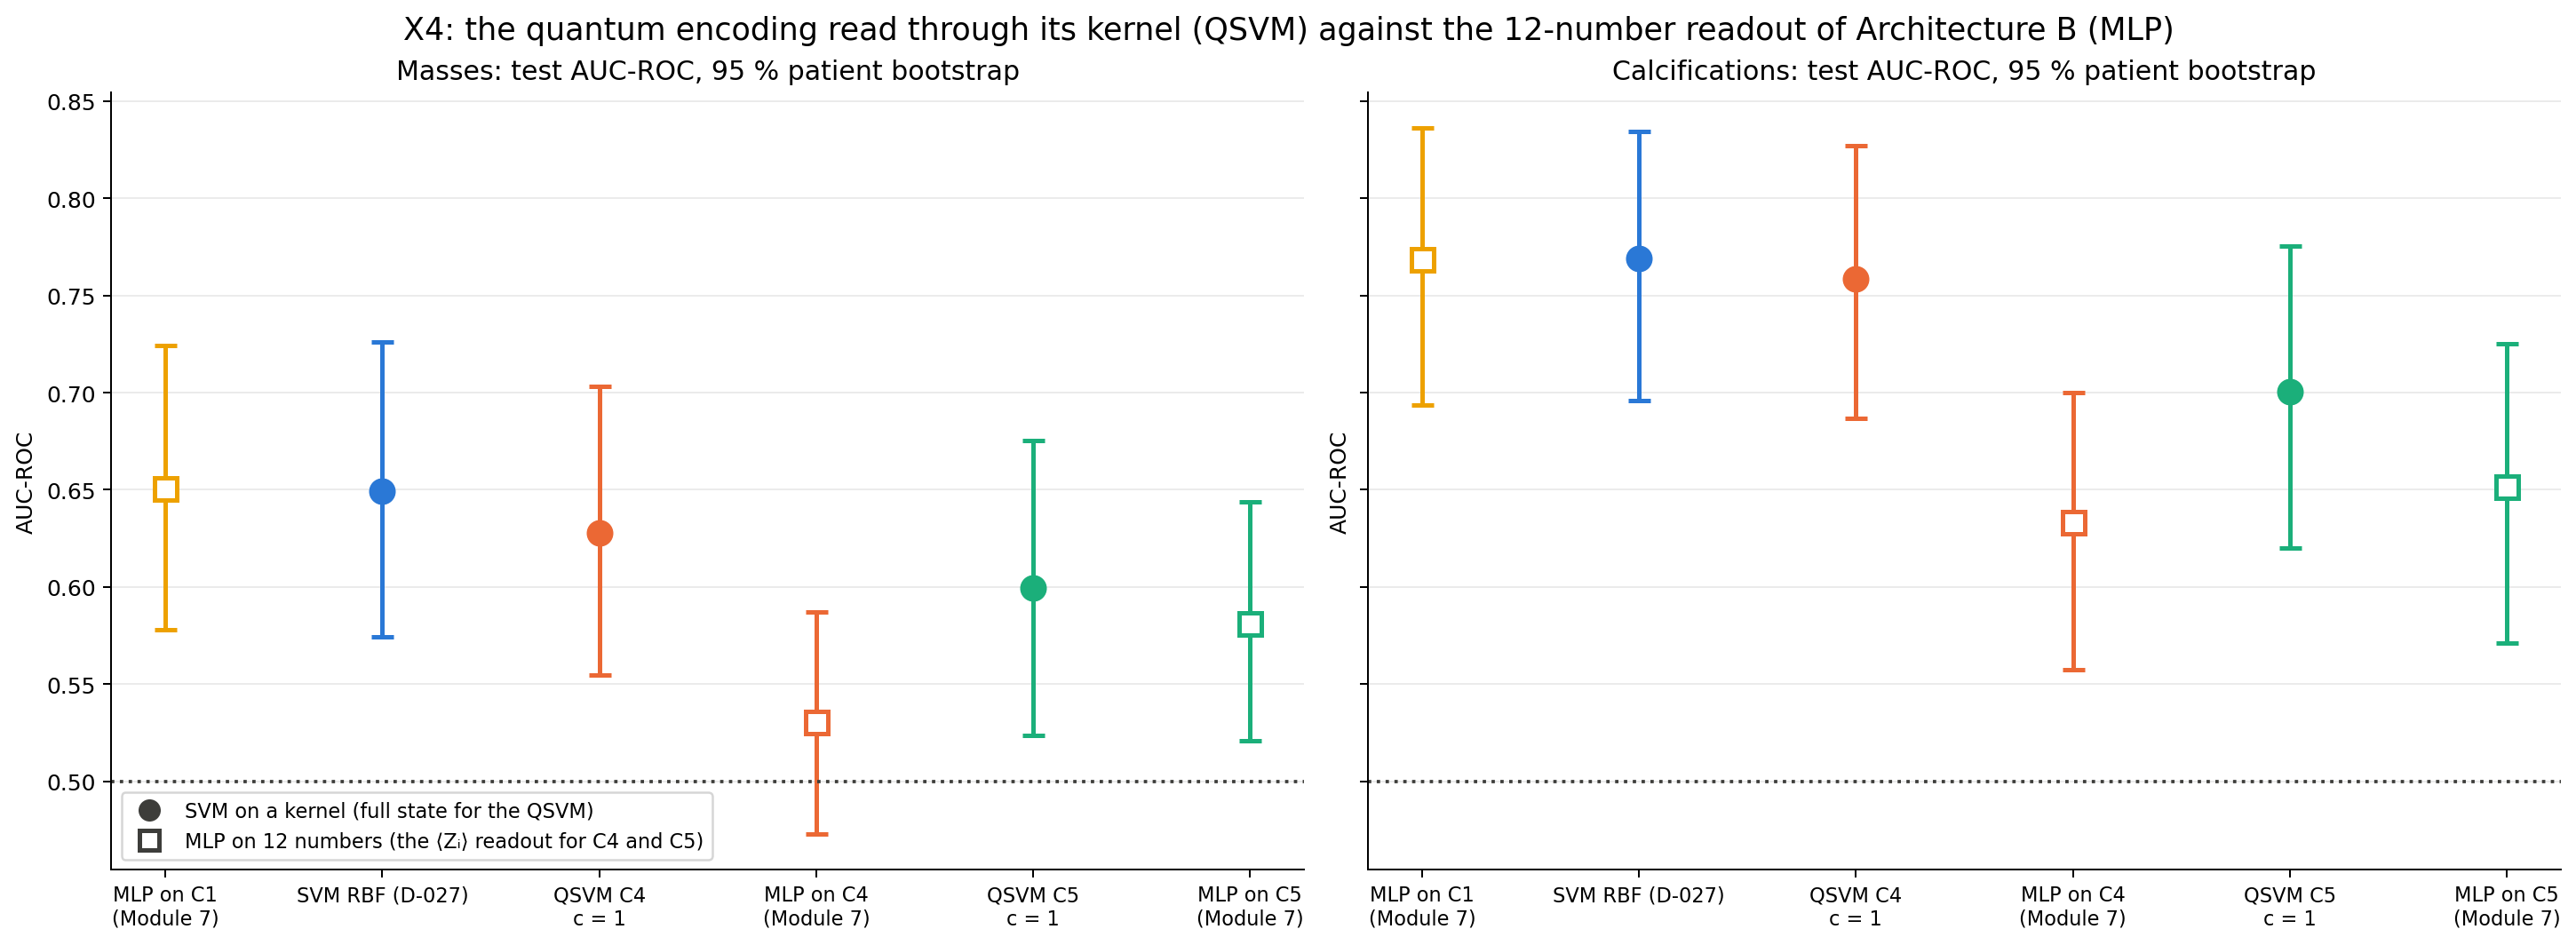
\includegraphics[width=\textwidth]{Figures/X4_qsvm_vs_readout.png}
\caption{Comparación entre el clasificador de kernel cuántico (QSVM), el clasificador de vectores de soporte clásico (SVM RBF) y la lectura mediante expectativas locales $\langle Z_i \rangle$ con red neuronal.}
\label{fig:x4_qsvm_vs_readout}
\end{figure}

% fuente: H-045; X4_67_features.csv, X4_test.csv, X4_test_diferencias.csv
La evaluación exploratoria incorporando la totalidad de las 67 características radiómicas extraídas tampoco evidencia ventaja computacional cuántica. El clasificador SVM RBF clásico sobre las 67 características obtiene un AUC de 0.649 en masas (diferencia de $-0.001$ frente a las 12 variables seleccionadas) y de 0.787 [0.73, 0.85] en calcificaciones ($+0.02$ [$-0.02$, $0.06$]). La codificación en amplitudes cuánticas sobre 7 qubits genera una matriz de kernel idéntica al cuadrado de la similitud coseno (un kernel polinomial clásico de segundo grado, con discrepancia numérica de $2 \times 10^{-16}$); este mapa alcanza un AUC de 0.795 [0.73, 0.85] en calcificaciones (sin superar significativamente al RBF clásico, con diferencia de $+0.008$) y de 0.599 en masas (diferencia de $-0.05$ [$-0.10$, $0.00$]). Por su parte, la codificación angular en producto tensorial sobre 67 qubits se concentra enteramente a escala $c = 1$ (mediana fuera de la diagonal de 0.0000), mientras que a escalas reducidas $c$ aproxima analíticamente a un kernel gaussiano clásico ($\prod \cos^2(c \Delta_i) \approx \exp(-c^2 \|\Delta\|^2)$) rindiendo a la par del SVM clásico. Un mapa con entrelazamiento completo sobre 67 variables requeriría simular $2^{67} \approx 1.5 \times 10^{20}$ amplitudes, resultando intratable clásicamente e inaccesible físicamente debido a la concentración exponencial \cite{Thanasilp2024}.

\begin{figure}[htbp]
\centering
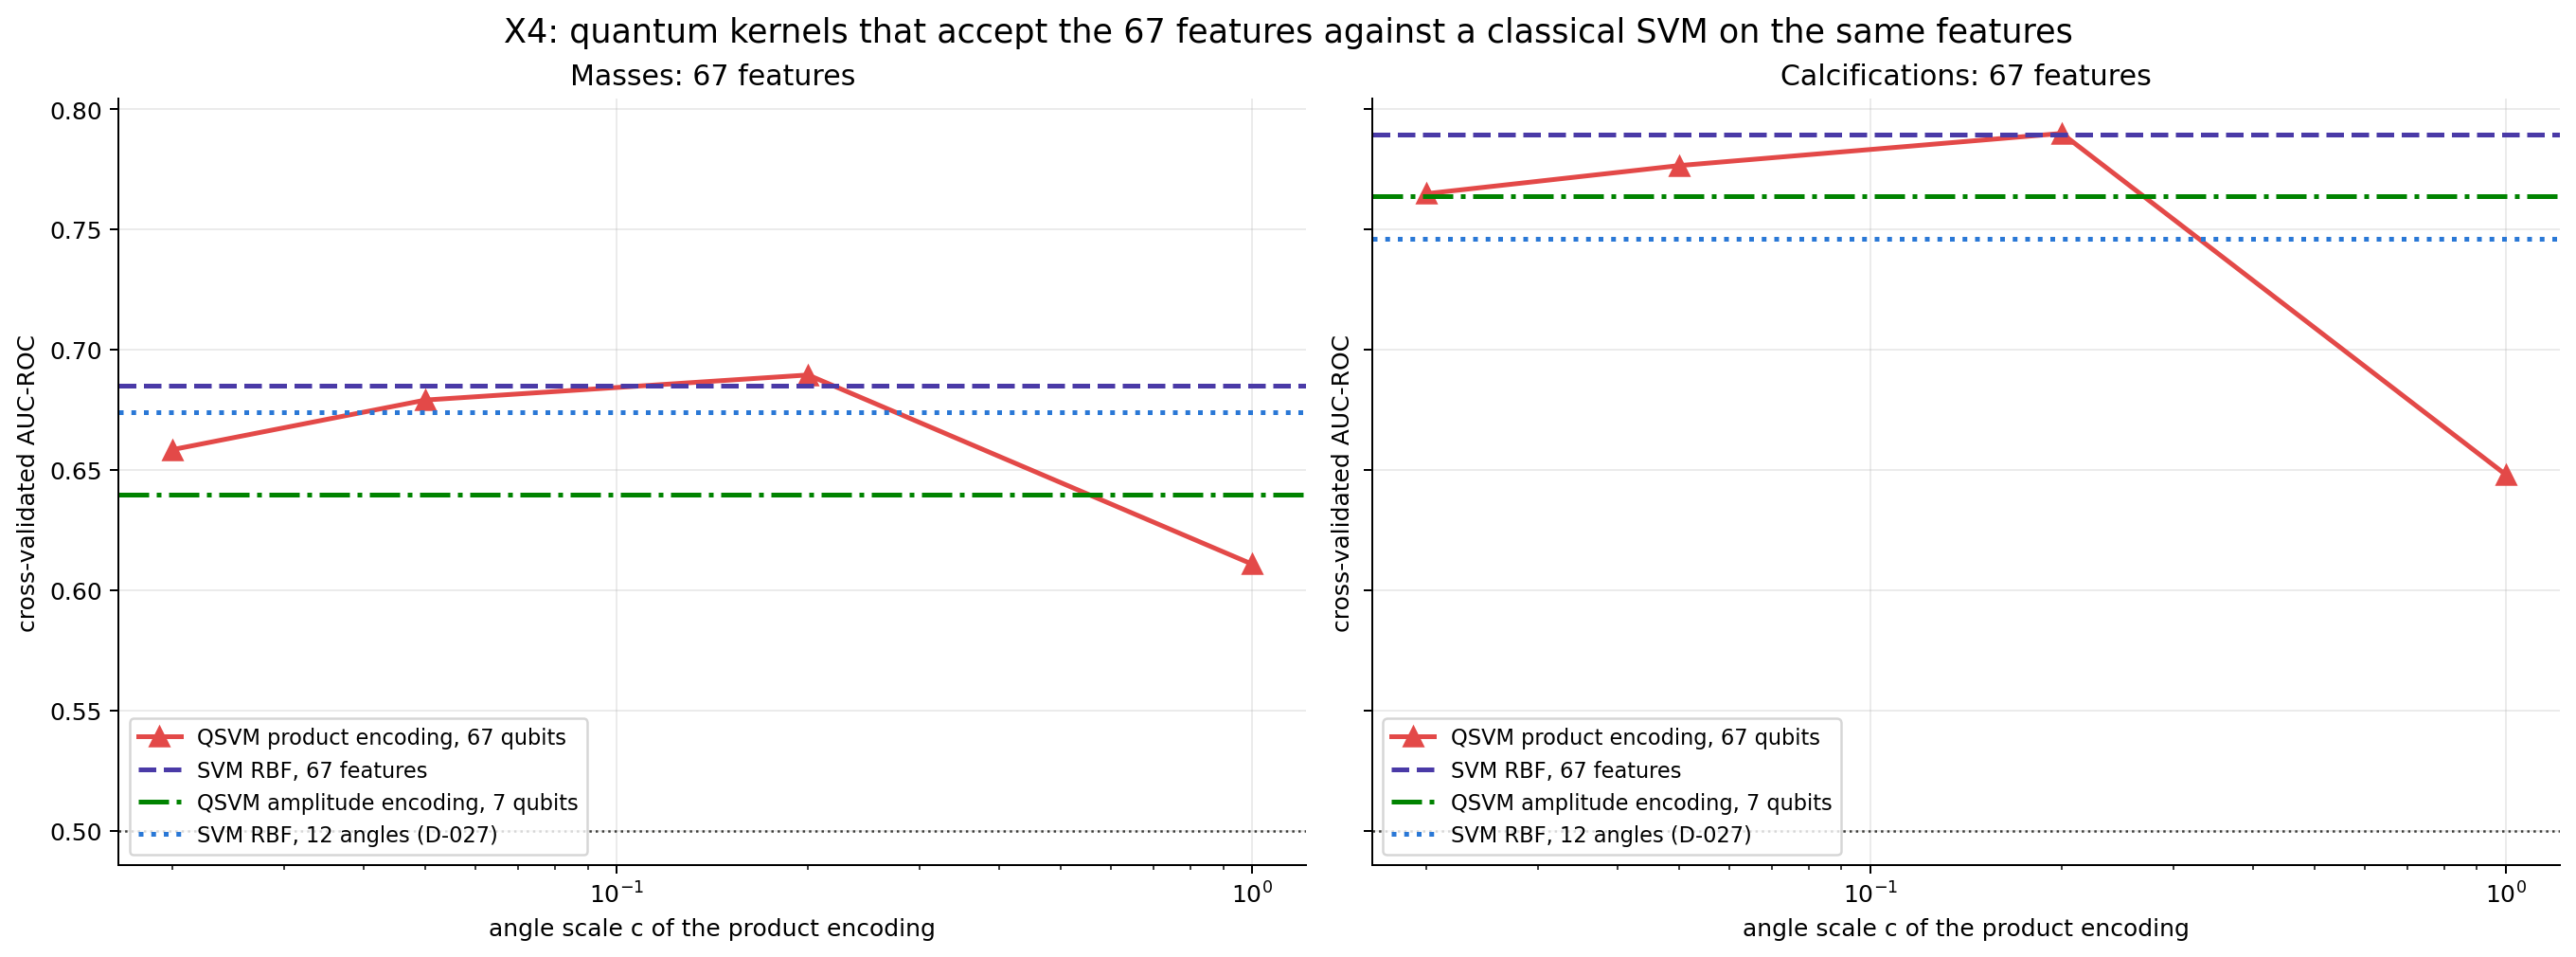
\includegraphics[width=\textwidth]{Figures/X4_67_features.png}
\caption{Rendimiento de clasificación en el conjunto de prueba al emplear las 67 características radiómicas bajo kernels clásicos, codificación en amplitudes y mapas angulares.}
\label{fig:x4_67_features}
\end{figure}

% fuente: H-046; X5_auditoria.csv
Con el fin de verificar que la ausencia de ventaja cuántica no se deba a anomalías de implementación, se llevó a cabo una auditoría del pipeline experimental, que superó las 25 verificaciones programadas. Estas pruebas confirmaron la integridad de las particiones y etiquetas de los 3\,568 casos reconstruidos directamente desde los metadatos originales sin filtración entre conjuntos, la reproducibilidad analítica del kernel cuántico por circuitos frente al cálculo por vectores de estado ($6 \times 10^{-11}$), la concordancia idéntica entre la implementación propia de SVM y la librería Qiskit Machine Learning, y la invarianza del kernel ante permutaciones de variables. Aunque dicha auditoría interna fue formulada por el propio equipo de trabajo, la reproducibilidad externa queda respaldada por la re-ejecución automatizada e integral del pipeline en un entorno limpio independiente, en la cual cero cuadernos presentaron fallos y los 81 archivos de resultados junto con los 10\,704 archivos de imágenes preprocesadas resultaron idénticos bit a bit.

% fuente: H-047; X6_anidada.csv, X6_diferencias.csv, X6_test.csv, X6_rejilla_candidatos.csv
Bajo un protocolo simétrico de validación cruzada anidada (tres pliegues internos por paciente) diseñado para buscar activamente ventaja cuántica, se contrastaron familias extendidas de kernels cuánticos y clásicos. En este procedimiento se evaluó un conjunto asimétrico compuesto por 28 candidatos cuánticos frente a 12 clásicos (140 frente a 60 ajustes considerando los pliegues de validación), una asimetría deliberada que favorece la exploración del espacio de hipótesis cuántico frente al clásico y otorga un carácter conservador a los hallazgos. En validación cruzada anidada, los contendientes clásico y cuántico alcanzan un AUC de 0.677 frente a 0.651 en masas (diferencia de $-0.027$ [$-0.043$, $-0.009$]) y de 0.745 frente a 0.753 en calcificaciones ($+0.007$ [$-0.007$, $0.023$]). En la evaluación final sobre el conjunto de prueba, el mejor modelo clásico y el mejor modelo cuántico arrojan 0.652 frente a 0.656 en masas ($+0.004$ [$-0.023$, $0.033$]) y 0.760 frente a 0.755 en calcificaciones ($-0.005$ [$-0.032$, $0.022$]).

% fuente: H-047; X6_anidada.csv, X6_diferencias.csv, X6_geometria.csv
La configuración cuántica óptima seleccionada por el procedimiento anidado converge a la equivalencia funcional con el kernel clásico: selecciona el mapa ZZ completo con escala reducida ($c = 0.05$ y $c = 0.2$), régimen en el que los términos de entrelazamiento de segundo orden se vuelven despreciables y el comportamiento emula un kernel RBF clásico. Por su parte, la hipótesis de que un entrelazamiento lineal reduciría la concentración de fidelidades resultó refutada: la mediana del kernel se reduce a 0.0001 (frente a 0.002 en el mapa completo), aproximando estados producto cuya fidelidad decae exponencialmente. Asimismo, los kernels proyectados propuestos por Huang et al. \cite{huang2021power}, si bien elevan la diferencia geométrica $g$ a un rango de 6 a 9 y la dimensión efectiva a aproximadamente 10, obtienen el desempeño clasificatorio más deficiente sobre las etiquetas clínicas reales (AUC inferior en $-0.11$ en masas y $-0.06$ en calcificaciones respecto a los clásicos), confirmando que una separación geométrica elevada es condición necesaria pero no suficiente para obtener ventaja en generalización.

\begin{figure}[htbp]
\centering
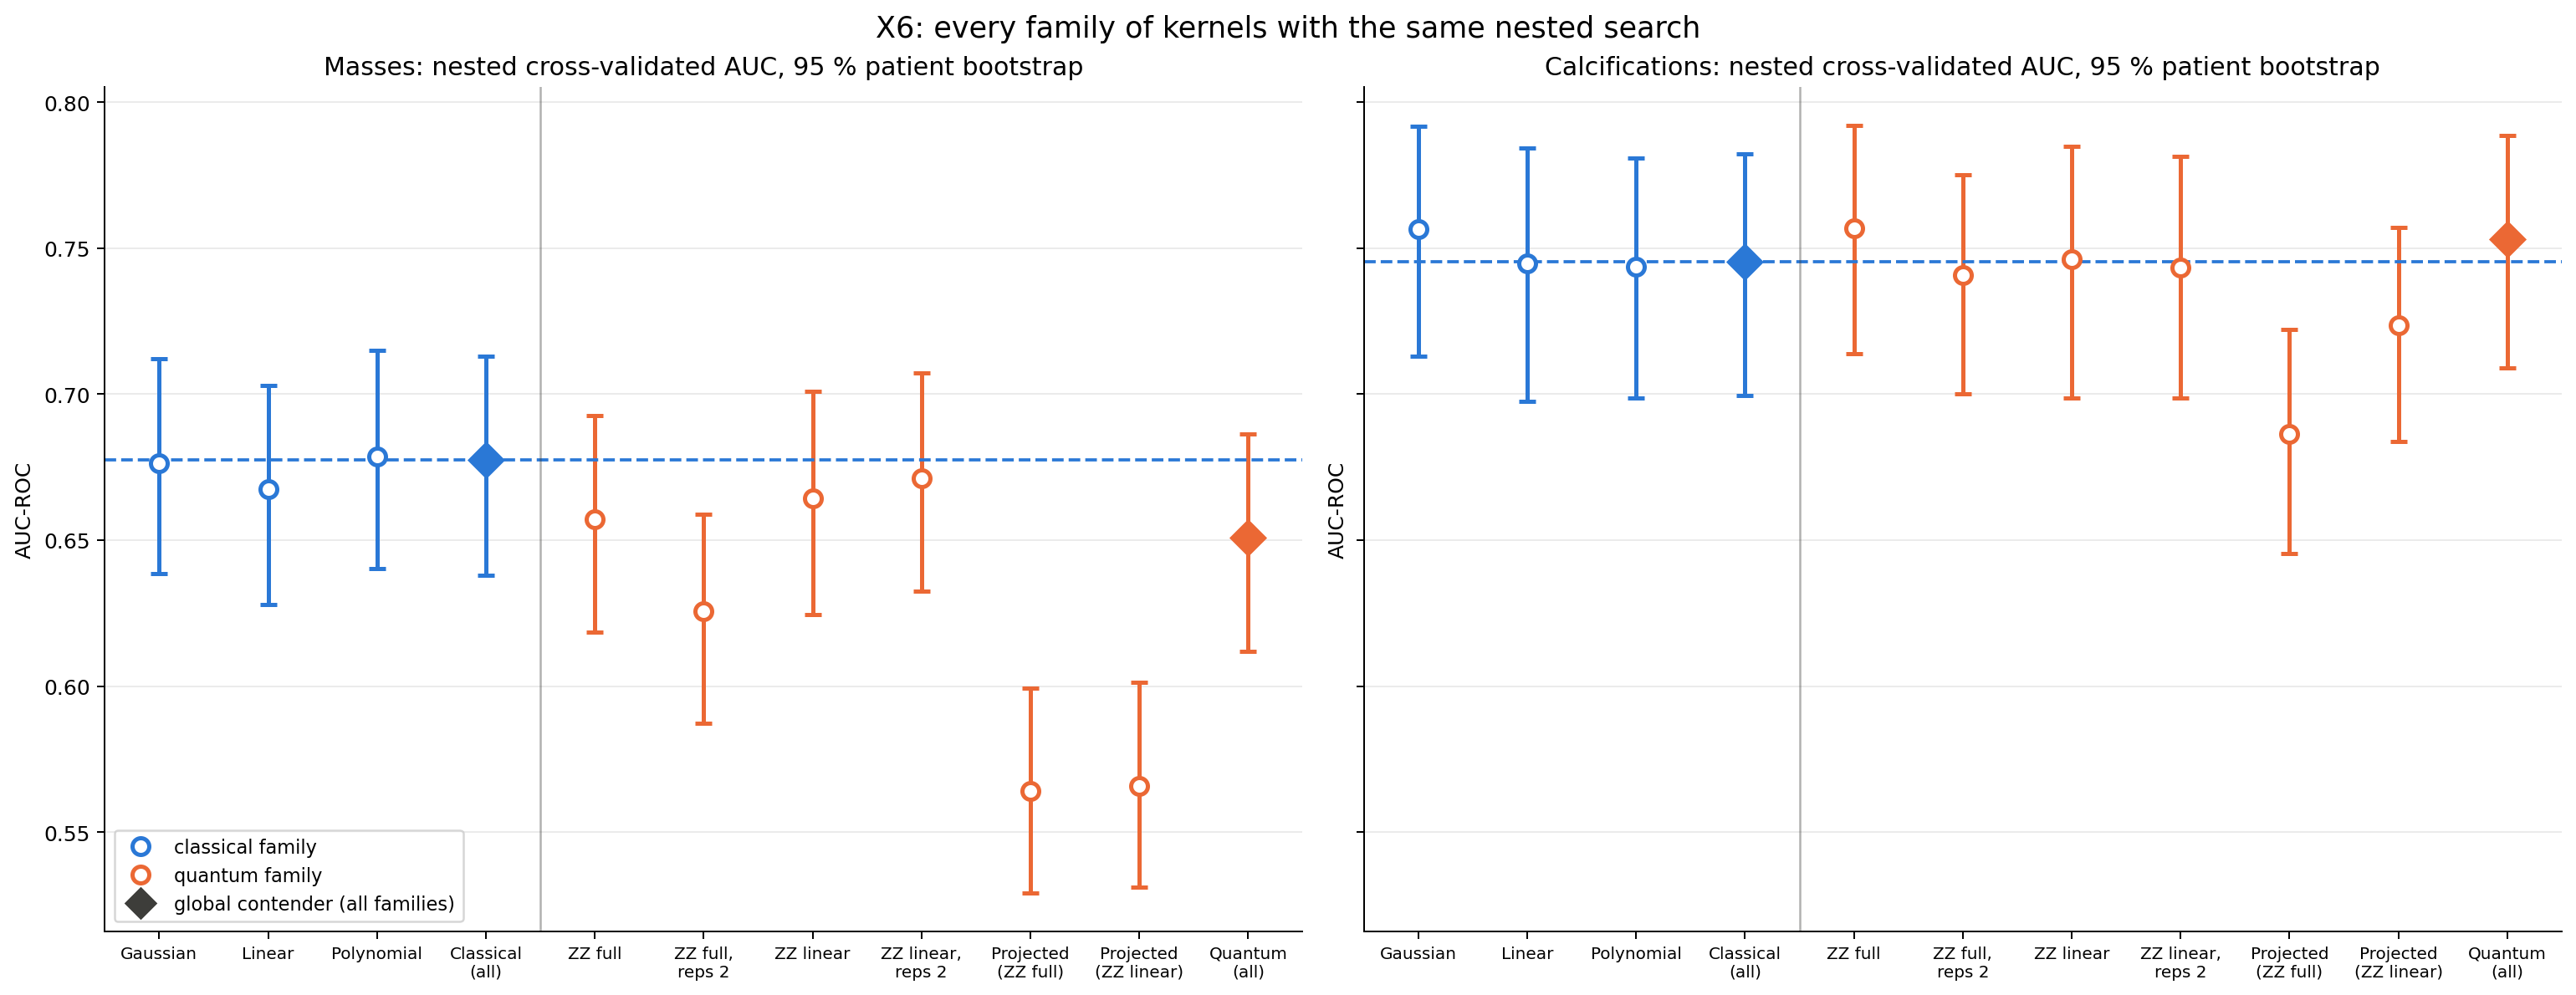
\includegraphics[width=\textwidth]{Figures/X6_nested_auc.png}
\caption{Búsqueda anidada sistemática de ventaja computacional cuántica: curvas de rendimiento en validación cruzada interna y evaluación pareada en el conjunto de prueba oficial.}
\label{fig:x6_nested_auc}
\end{figure}

% fuente: H-048; X6_etiquetas_construidas.csv
Para esclarecer si la ausencia de ventaja obedece al protocolo clasificatorio o a la estructura intrínseca del problema, se sintetizaron etiquetas artificiales alineadas geométricamente con el kernel cuántico conforme al procedimiento del Apéndice G de Huang et al. \cite{huang2021power} ($y = \sqrt{K_Q} \mathbf{v}$ binarizado por la mediana), empleando las mismas lesiones y características radiómicas del conjunto de datos. Bajo estas etiquetas sintéticas, el clasificador de kernel proyectado cuántico alcanza un AUC de 0.998 en masas y de 0.994 en calcificaciones, superando holgadamente al mejor clasificador clásico optimizado (0.800 en masas y 0.824 en calcificaciones), en agudo contraste con el rendimiento observado sobre las etiquetas diagnósticas reales (0.566 frente a 0.682 en masas; 0.667 frente a 0.759 en calcificaciones). Con el mapa ZZ completo, la ganancia sobre etiquetas sintéticas es menor (0.730 frente a 0.712 en masas; 0.829 frente a 0.807 en calcificaciones), acorde con su bajo valor de diferencia geométrica.

% fuente: H-048; X6_etiquetas_construidas.csv
Este contraste experimental demuestra que la ausencia de ventaja cuántica observada en este estudio es una propiedad de estas etiquetas diagnósticas clínicas al combinarse con estas 12 características radiómicas y estas familias de kernels cuánticos evaluadas (mapas ZZ con entrelazamiento completo o lineal, una o dos repeticiones, y kernels proyectados; nótese que el mapa Pauli Y-ZZ de C5 no formó parte de este barrido específico), y no una limitación del protocolo experimental. El esquema metodológico es plenamente capaz de detectar ventajas cuánticas pronunciadas cuando la función objetivo se encuentra alineada con la geometría del espacio de Hilbert inducido por el circuito.

\begin{figure}[htbp]
\centering
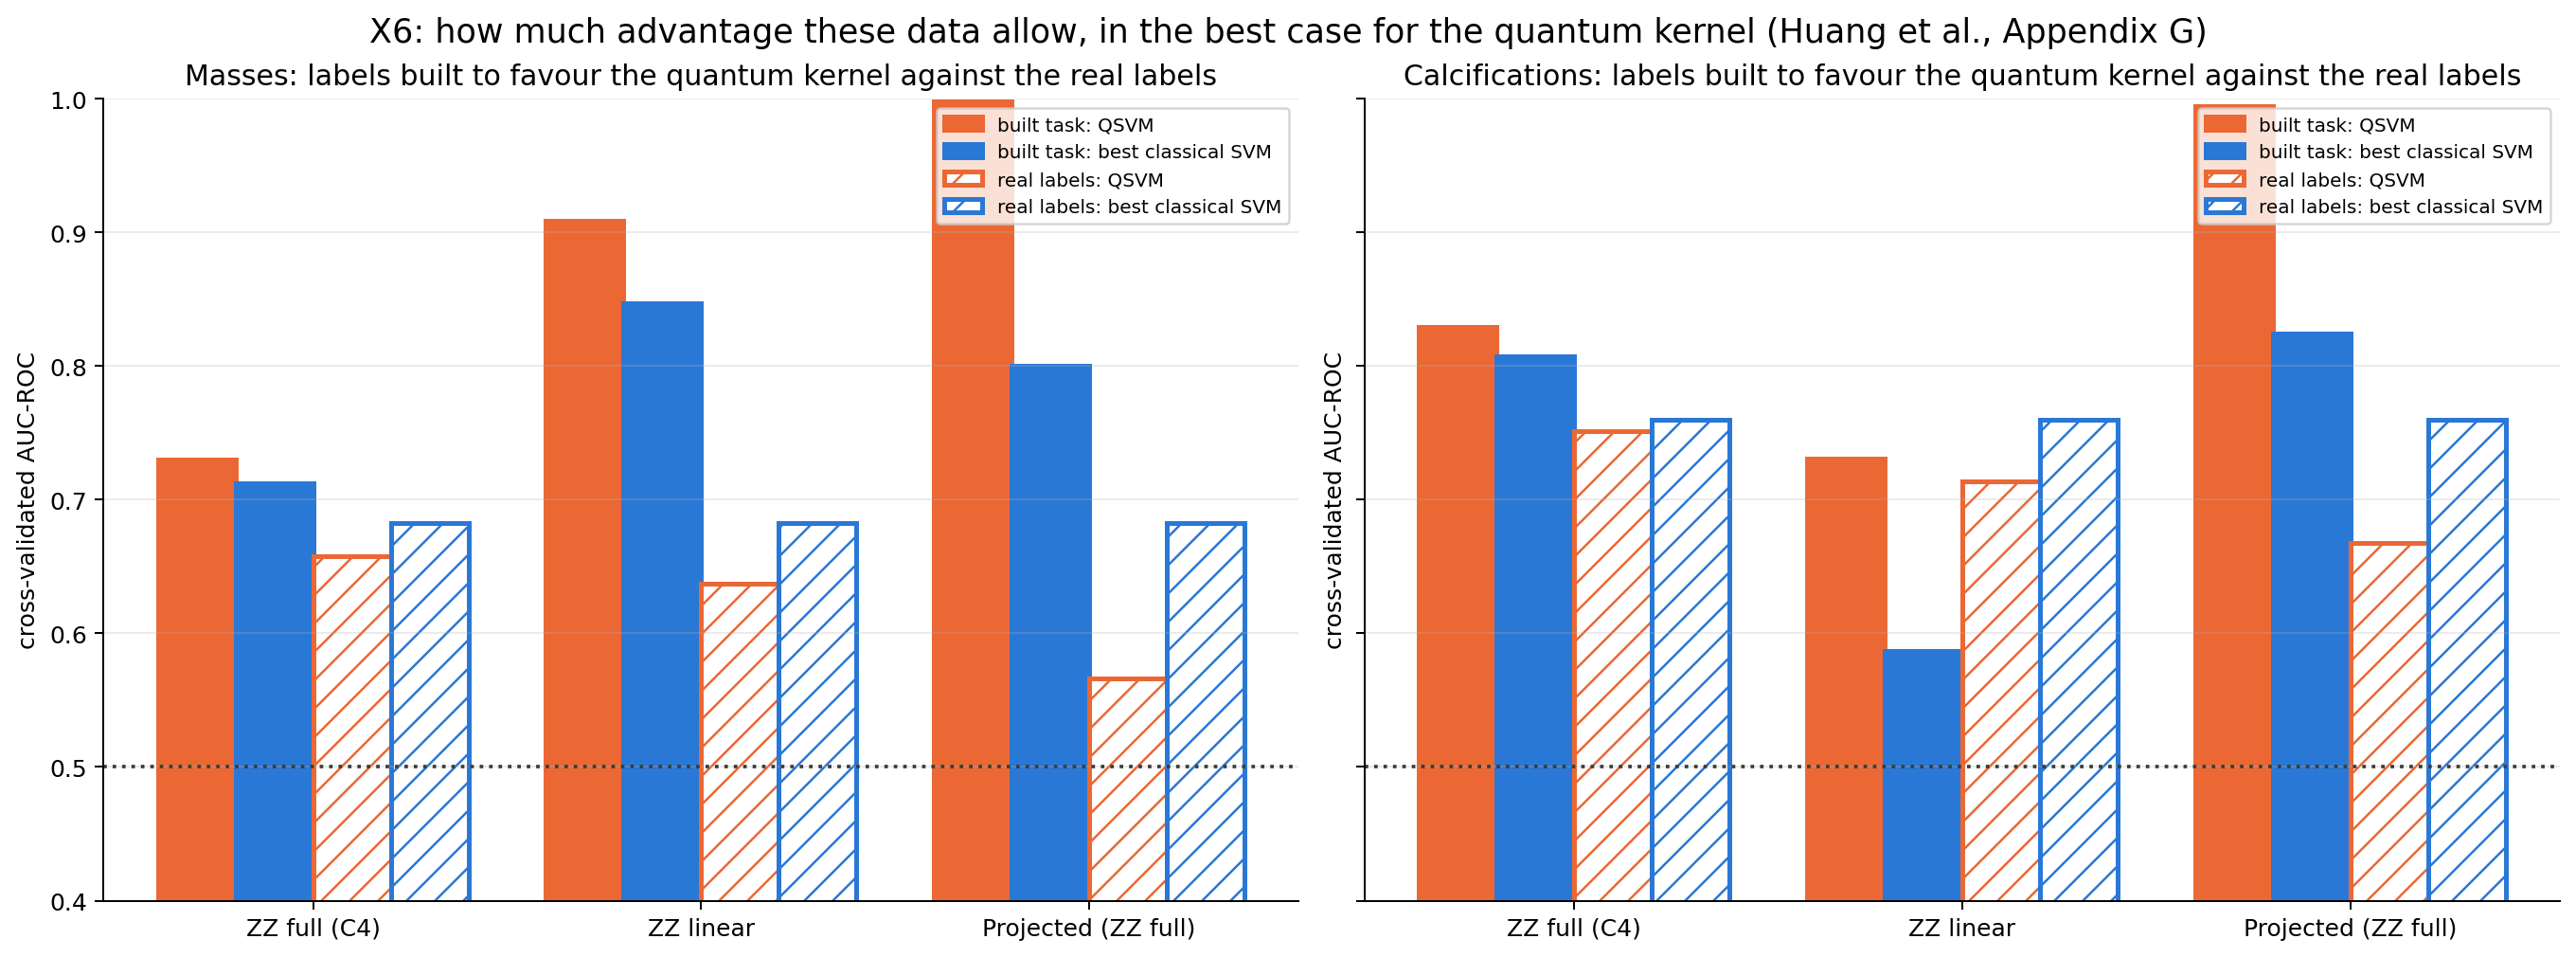
\includegraphics[width=\textwidth]{Figures/X6_built_labels.png}
\caption{Desempeño clasificatorio sobre etiquetas sintéticas diseñadas según la geometría cuántica en comparación con las etiquetas clínicas diagnósticas reales de CBIS-DDSM.}
\label{fig:x6_built_labels}
\end{figure}

% ---
% Reemplaza líneas 3458–3462 de Docs/Technical_Report.tex.
% Decisiones y hallazgos que lo respaldan: D-039, D-040, H-049, H-050.
% ---

\subsection{Evaluación comparativa}

% fuente: H-049; 8_spearman.csv, 8_rangos.csv
\input{tablas/m8_spearman}

% fuente: H-049; 8_spearman.csv, 8_rangos.csv, 8_spearman_nula.csv
La correlación de rangos de Spearman ($\rho_s$) entre los ordenamientos de separabilidad espacial calculados en el espacio de \textit{embedding} y el orden de desempeño clasificatorio en el conjunto de prueba se presenta en el cuadro~\ref{tab:m8_spearman}. Conforme al diseño metodológico, dicho coeficiente se evalúa de manera descriptiva: para $n = 5$ condiciones existen únicamente $5! = 120$ permutaciones posibles, y dado que las condiciones clásicas C1 y C2 empatan de forma exacta en toda métrica geométrica afín por construcción, el valor máximo teóricamente alcanzable es $\rho_s = 0.975$, cuya probabilidad nula exacta bilateral es $p = 4/120 \approx 0.033$. En la muestra primaria de 200 lesiones a $k = 12$, los coeficientes observados son positivos en su totalidad: en masas, el índice de Davies--Bouldin arroja $\rho_s = 0.718$ ($p = 0.167$), la razón de Fisher $J$ obtiene $\rho_s = 0.821$ ($p = 0.133$) y la alineación KTA lineal registra $\rho_s = 0.718$ ($p = 0.167$); en calcificaciones, Davies--Bouldin y KTA lineal alcanzan el acuerdo máximo posible con $\rho_s = 0.975$ ($p = 0.033$), mientras que Fisher $J$ registra $\rho_s = 0.667$ ($p = 0.267$).

% fuente: H-049; 8_spearman.csv, 8_rangos.csv
Al considerar el análisis de sensibilidad exhaustivo sobre los 48 coeficientes de correlación calculados (combinando tres métricas de separabilidad, dos tamaños de muestra, dos evaluaciones de clasificación y los valores $k \in \{8, 12\}$), la totalidad de los valores se mantiene estrictamente positiva en el rango de 0.67 a 0.97. En todas las instancias evaluadas, los ordenamientos sitúan sin excepción al bloque de las tres condiciones clásicas (C1, C2 y C3) por delante del bloque de representaciones cuánticas (C4 y C5). Las fluctuaciones menores observadas al interior de cada bloque reflejan ruido numérico propio del entrenamiento. Asimismo, en el espacio de kernels ($n = 3$), el kernel RBF clásico lidera tanto en alineamiento de matrices como en clasificación con SVM respecto a las variantes cuánticas C4 y C5. Estos resultados confirman que las métricas de separabilidad geométrica reflejan adecuadamente la capacidad clasificatoria ulterior, evidenciando de manera coherente la ausencia de beneficio clasificatorio derivado de la transformación cuántica.

\begin{figure}[htbp]
\centering
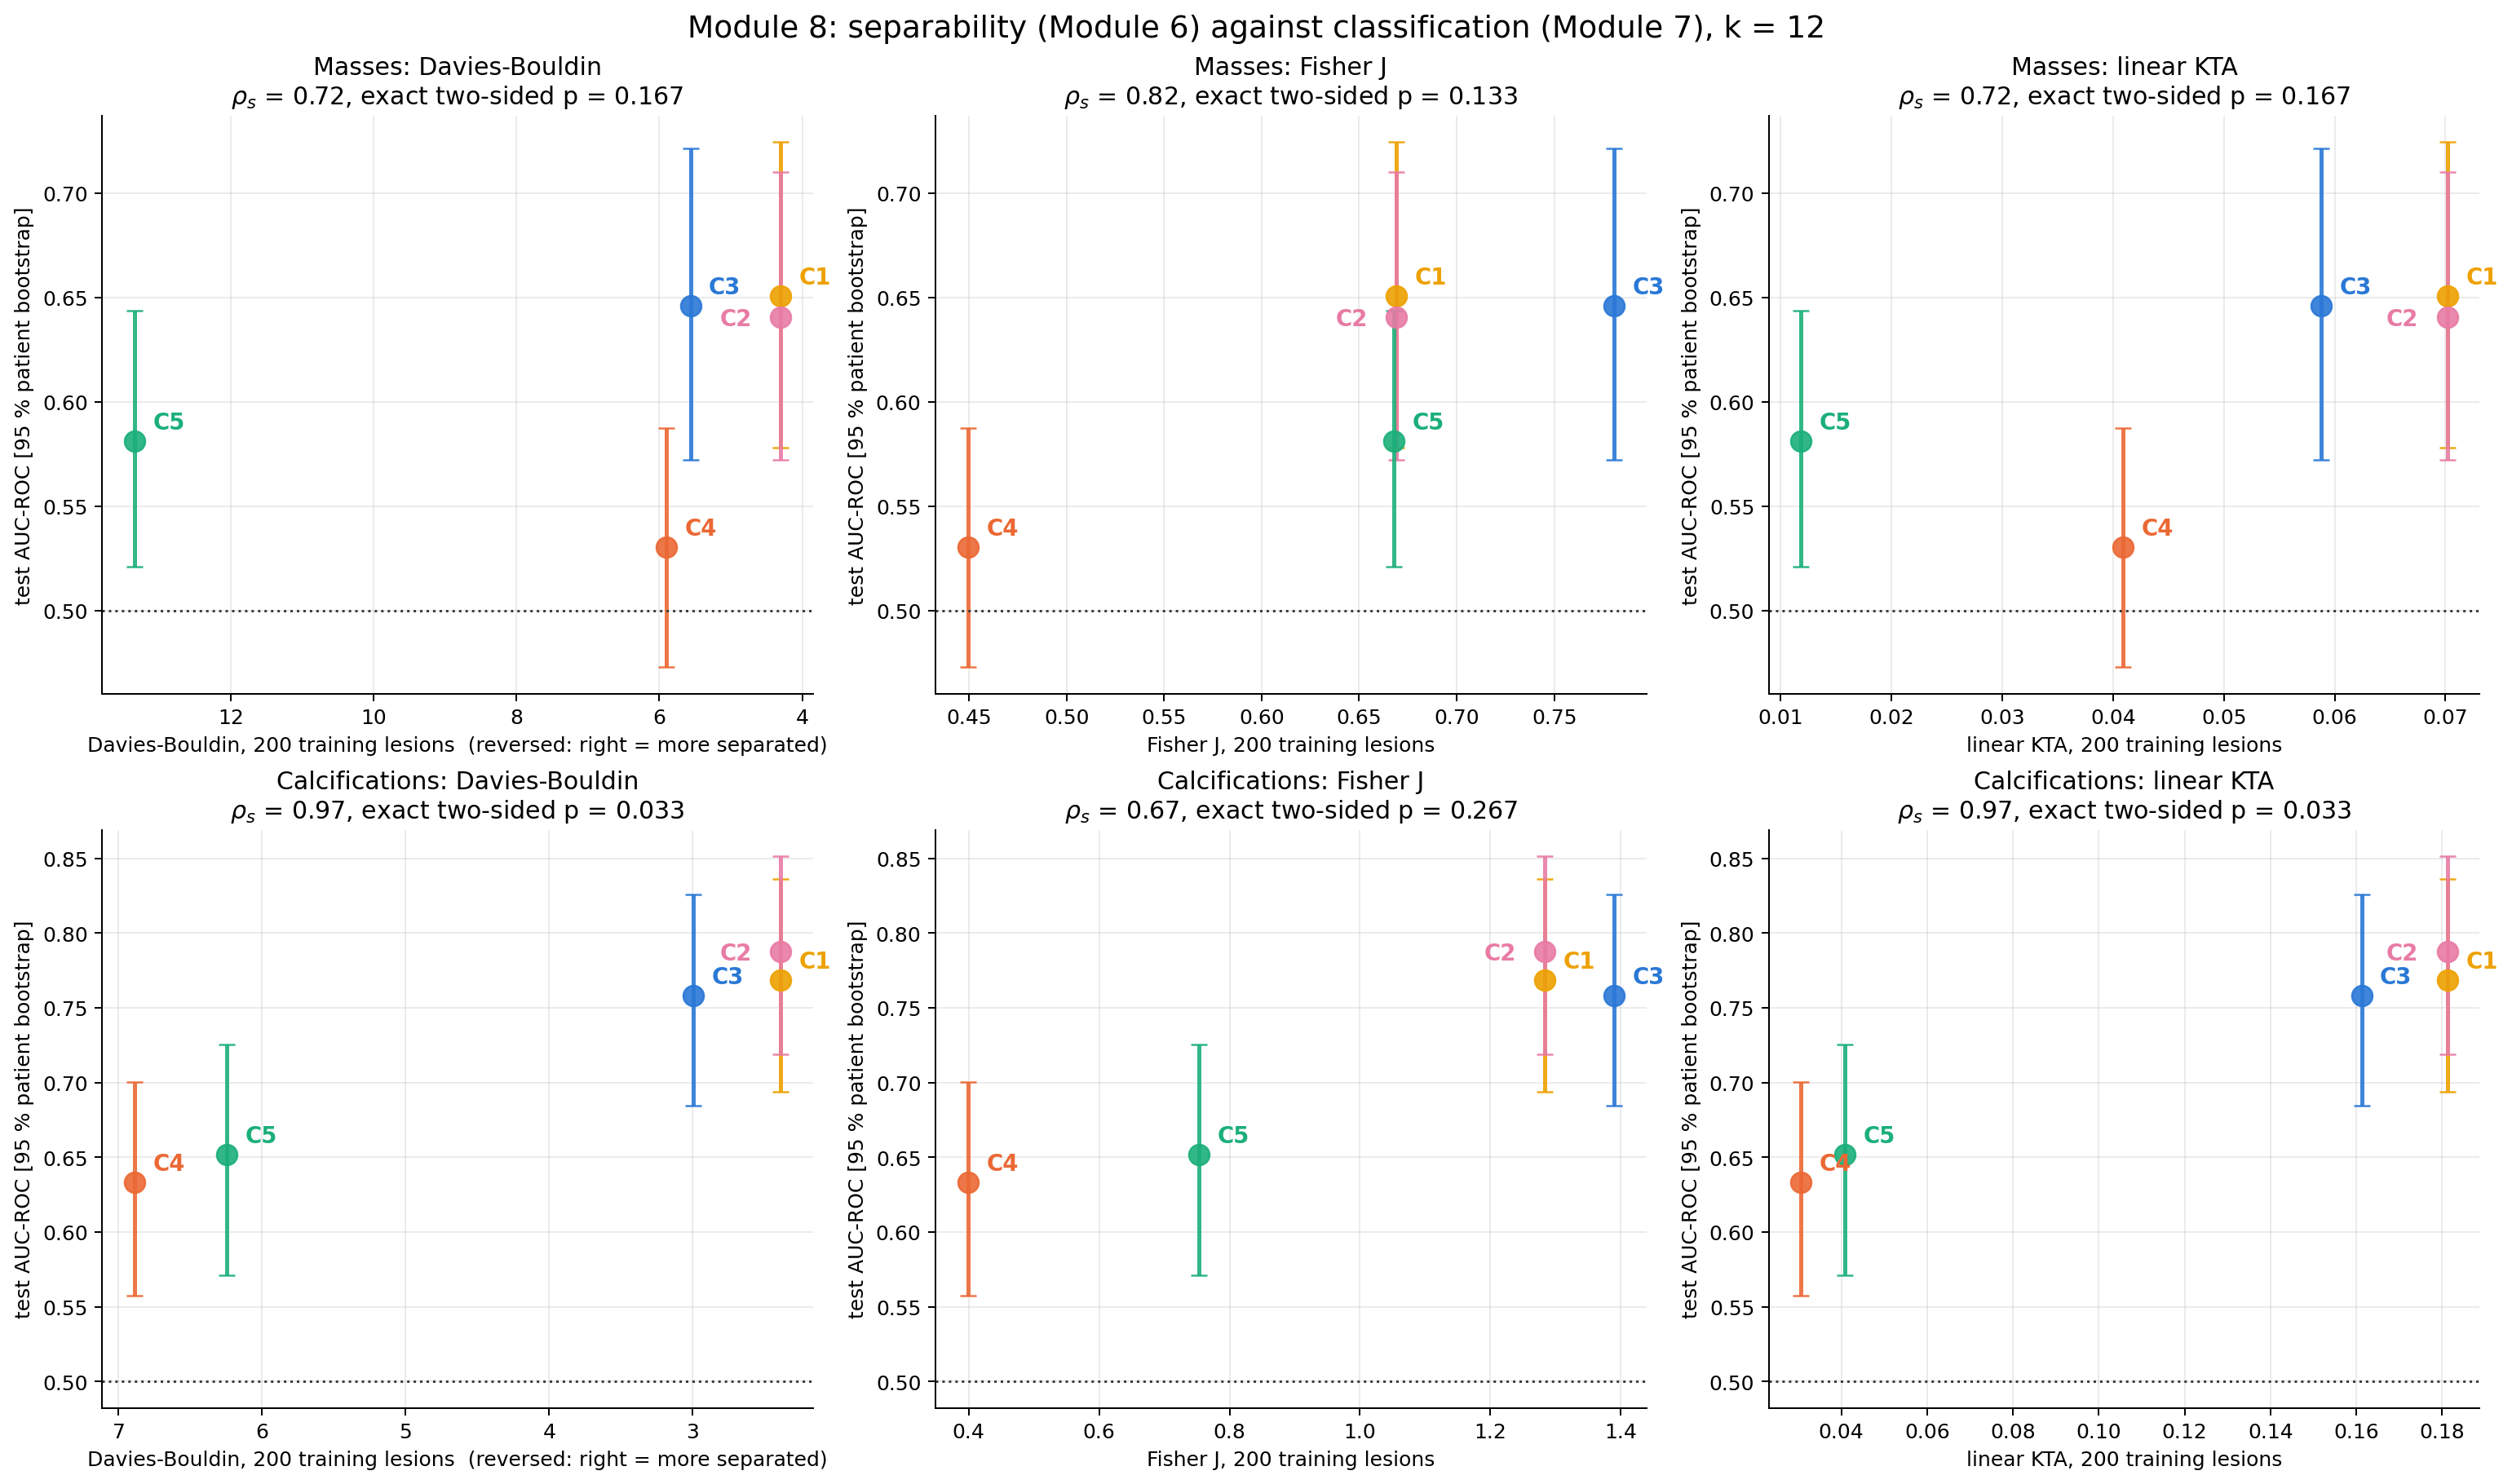
\includegraphics[width=\textwidth]{Figures/M8_spearman.png}
\caption{Correlación de Spearman entre los ordenamientos de separabilidad del espacio de estados y el desempeño de clasificación en el conjunto de prueba oficial.}
\label{fig:m8_spearman}
\end{figure}

\begin{figure}[htbp]
\centering
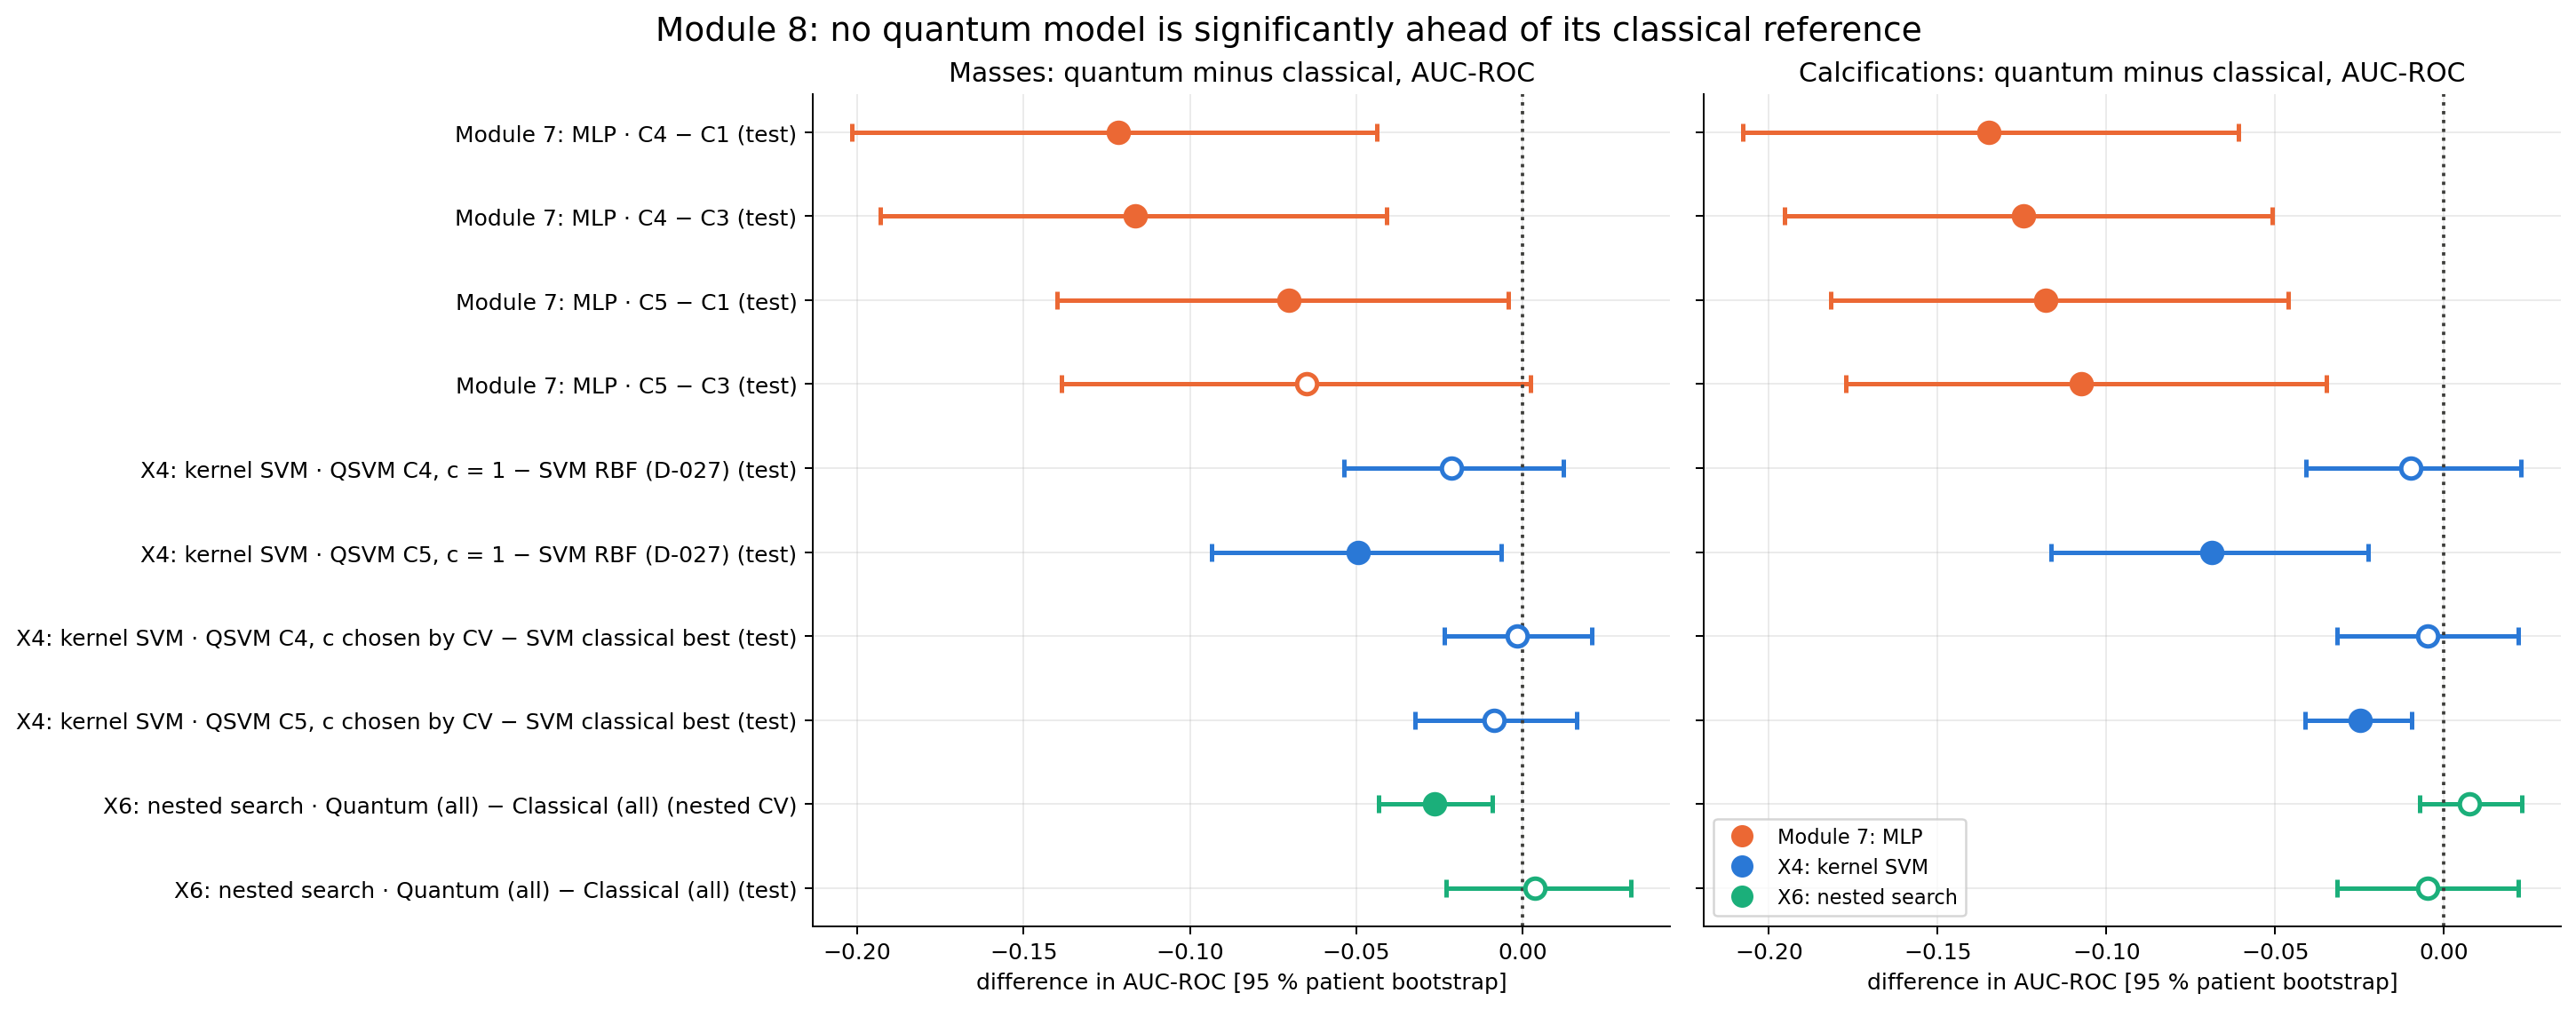
\includegraphics[width=\textwidth]{Figures/M8_classical_vs_quantum.png}
\caption{Dispersión bivariada y contraste pareado de métricas de separabilidad frente al AUC de clasificación entre condiciones clásicas y cuánticas.}
\label{fig:m8_classical_vs_quantum}
\end{figure}

% fuente: H-050; 8_descriptores_radiologo.csv, 8_masas_vs_calcificaciones.csv
La aparente discordancia observada entre el análisis exploratorio inicial ---donde las masas exhibían patrones morfológicos distintivos que sugerían una mayor separabilidad que las calcificaciones--- y el rendimiento del clasificador final se explica por la naturaleza de los descriptores radiómicos extraídos. Al evaluar una regresión logística sobre los descriptores categóricos anotados por el médico radiólogo en CBIS-DDSM (forma y margen en masas; tipo morfológico y distribución en calcificaciones), las masas constituyen el subconjunto más separable, alcanzando un AUC en validación cruzada de 0.872 frente a 0.825 en calcificaciones. Estos descriptores radiológicos operan como una referencia clínica interpretativa y no como un sistema automatizado competidor, dado que fueron asignados mediante inspección médica experta.

% fuente: H-050; 8_descriptores_radiologo.csv, 8_masas_vs_calcificaciones.csv
Al sustituir el juicio experto por las características radiómicas cuantitativas calculadas en el pipeline, el orden de dificultad se invierte: las 67 características radiómicas recuperan un AUC de 0.800 en calcificaciones (muy próximo a los 0.825 del radiólogo), pero descienden a 0.693 en masas (lejos de los 0.872 del radiólogo). Con las 12 características seleccionadas en M4, el AUC se sitúa en 0.745 en calcificaciones y en 0.668 en masas. Esta discrepancia revela que la mayor dificultad clasificatoria en masas es una propiedad de las variables radiómicas cuantitativas estándar empleadas, las cuales resumen la textura y contorno global sin capturar con la misma fidelidad los detalles finos de espiculación perilesional que distingue el ojo experto. Por otra parte, el impacto de la representación cuántica resulta equivalente en ambos subconjuntos: la brecha C4 $-$ C1 es de $-0.12$ en masas y de $-0.14$ en calcificaciones, con medianas del kernel análogas (0.002 a 0.003 en C4; 0.00003 en C5) y diferencias geométricas similares ($g$ entre 1.4 y 1.7), demostrando que la asimetría observada entre patologías obedece a la señal radiómica clásica y no al comportamiento del circuito cuántico.

% ---
% Reemplaza líneas 3458–3462 de Docs/Technical_Report.tex.
% Decisiones y hallazgos que lo respaldan: D-040, H-019, H-032, H-037, H-051, H-052.
% ---

\subsection{Restricciones del simulador (OE-6)}

% fuente: H-051; 8_oe6_qubits.csv, 8_oe6_resumen.csv
Para evaluar los límites de viabilidad computacional (OE-6), se cronometró la simulación de estados del circuito cuántico de C4 mediante \texttt{AerSimulator} en modo vector de estado sobre un procesador Apple M3 con 16\,GiB de memoria RAM unificada para valores pares de $k$ entre 8 y 28. A partir de estas mediciones se proyectaron los techos operacionales bajo el criterio de viabilidad de ejecución en menos de 24 horas y un consumo máximo correspondiente a la mitad de la memoria RAM disponible (8\,GiB). El almacenamiento de un único vector de estado en memoria ($16 \times 2^k$ bytes) resulta viable hasta $k = 29$ qubits. La extracción completa de representaciones de todas las lesiones del conjunto en 24 horas admite entre 25 y 26 qubits según la carga de la máquina. El cómputo de la matriz de kernel de $200 \times 200$ mediante el protocolo físico de \textit{compute-uncompute} soporta entre 22 y 23 qubits según la carga de la máquina, mientras que el cálculo con almacenamiento simultáneo de todos los vectores de estado en memoria alcanza hasta $k = 21$ qubits. Finalmente, el entrenamiento variacional de $\boldsymbol\theta$ por \textit{parameter-shift} (50 épocas, un mapa cuántico) únicamente resulta factible hasta 14--15 qubits según la carga de la máquina. A $k = 12$, el tiempo de cálculo por muestra fue de 3\,ms con \texttt{AerSimulator}, 8\,ms mediante el cálculo analítico de vector de estado y 93\,ms mediante la primitiva de alto nivel \texttt{EstimatorQNN}.

% fuente: H-051, H-032, H-054; 8_oe6_qubits.csv, 8_oe6_resumen.csv, X8_costo_gradiente.csv
El coste computacional escala como $2^k$: a partir de 20 qubits, el tiempo se multiplica por aproximadamente 1.9 por cada qubit adicional, con unos 75\,s por estado a $k = 28$; otras ejecuciones del mismo barrido dieron entre 46 y 152\,s, según la carga de la máquina. El factor que condicionó de forma determinante el diseño experimental no fue el número de qubits disponibles para almacenar el estado ($k = 12$ se sitúa holgadamente por debajo del límite de 25--26 qubits), sino el cálculo de gradientes. La estimación exacta de gradientes mediante la regla de \textit{parameter-shift} requiere 48 evaluaciones de circuito por lesión a $k = 12$; medido en el simulador con valores exactos, son 5.16\,s por lesión y unas 205~h por \textit{feature map} para 50 épocas sobre las 2\,864 lesiones de entrenamiento. Por su parte, el atajo computacional implementado mediante \texttt{FidelityStatevectorKernel} (que evalúa la matriz de $200 \times 200$ en 1.5\,s mediante productos internos vectoriales frente a los 41 minutos proyectados para circuitos independientes) solo existe en simulación clásica gracias al conocimiento simultáneo de todas las amplitudes y es físicamente irrealizable en hardware cuántico, donde cada fidelidad debe estimarse mediante medición repetida de circuitos \textit{compute-uncompute}.

\begin{figure}[htbp]
\centering
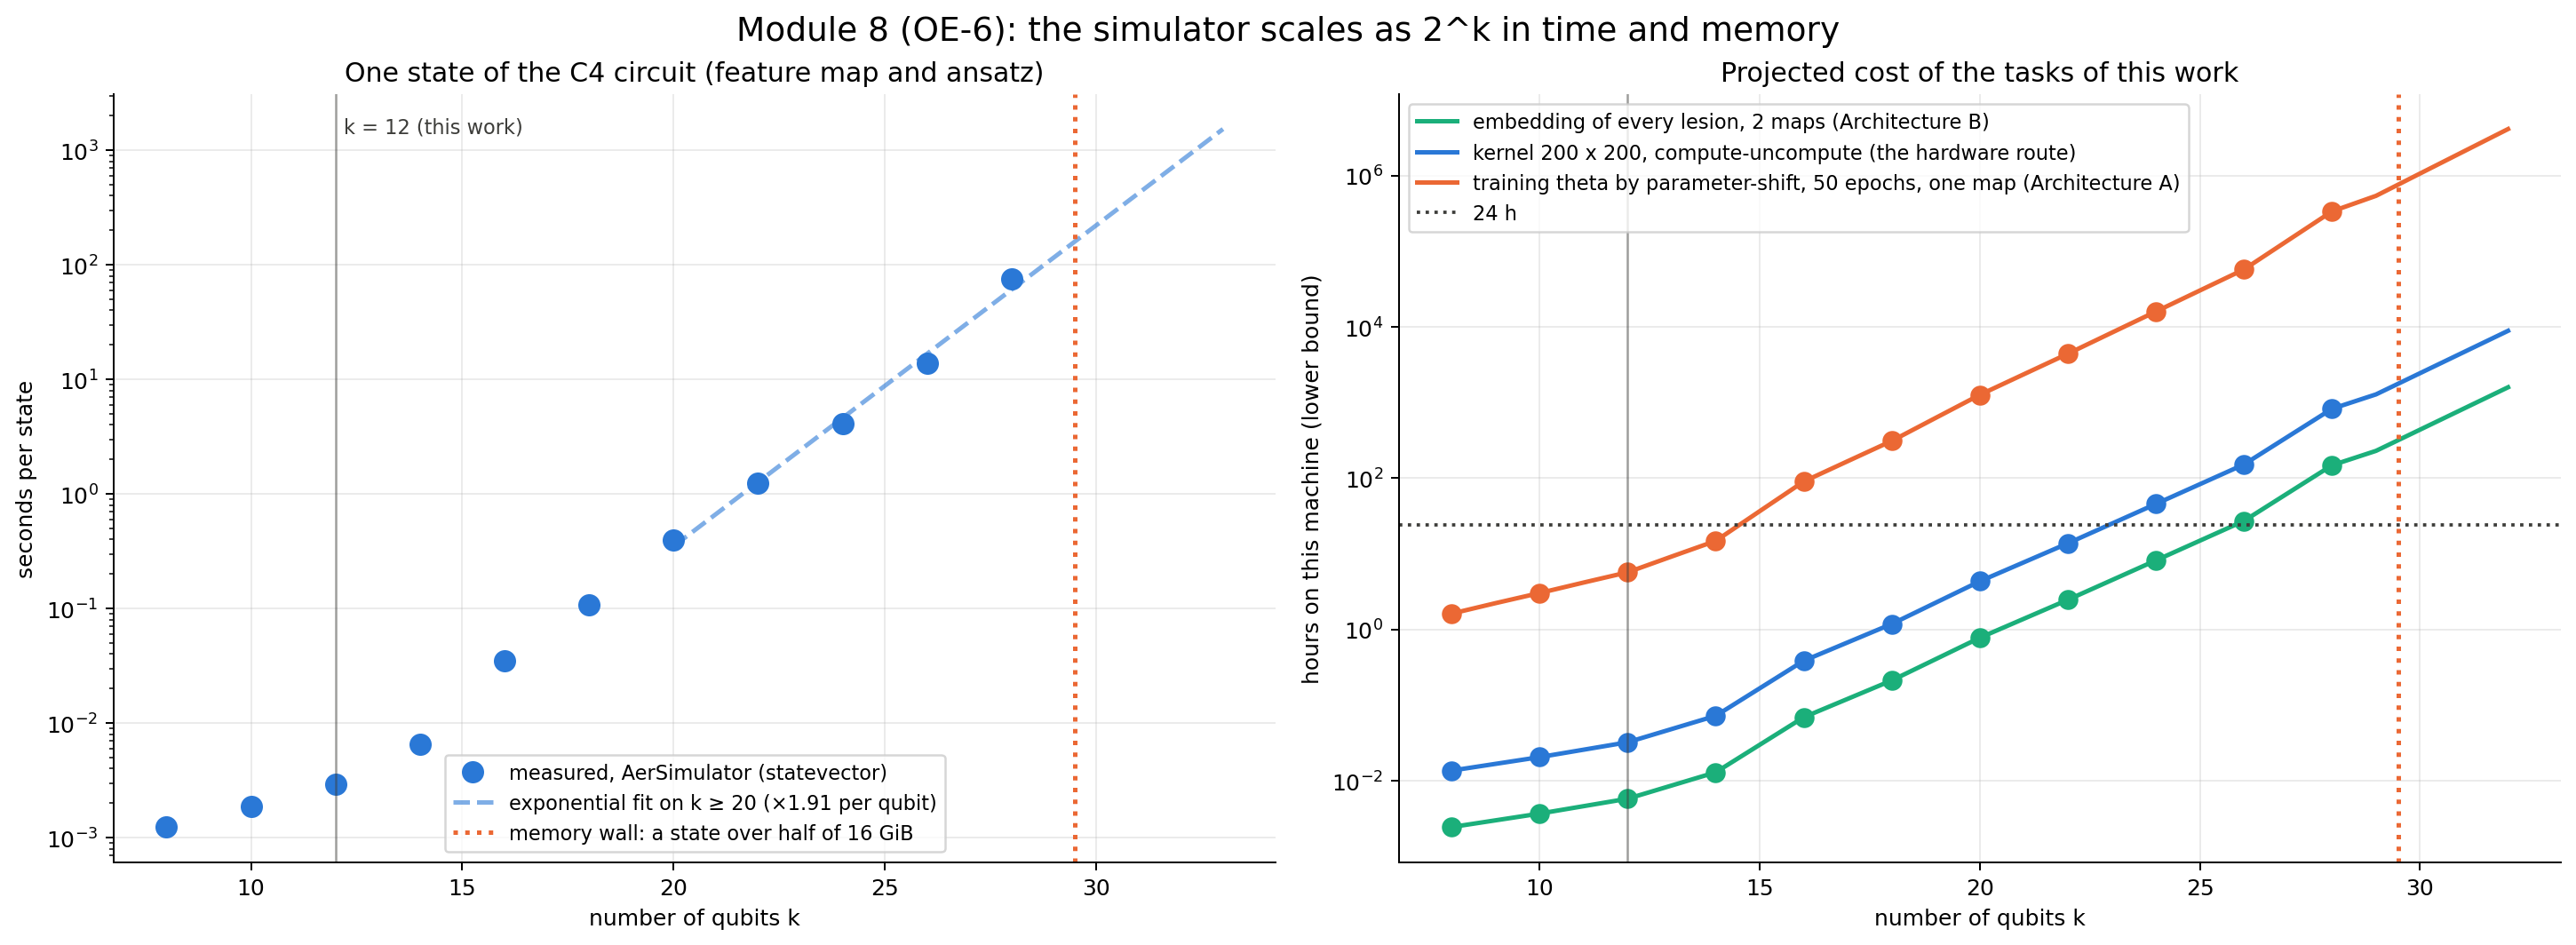
\includegraphics[width=\textwidth]{Figures/M8_oe6_qubits.png}
\caption{Escalabilidad computacional del simulador de vectores de estado en función del número de qubits ($k$) y proyección de límites temporales y de memoria para tareas del pipeline.}
\label{fig:m8_oe6_qubits}
\end{figure}

% fuente: H-052, H-019, H-037; 8_oe6_shots_embedding.csv, 8_oe6_shots_kernel.csv, 8_oe6_resumen.csv
El impacto del número finito de disparos (\textit{shots}) sobre las representaciones locales $\langle Z_i \rangle$ y las matrices de kernel se modeló mediante muestreo multinomial ideal sobre las probabilidades teóricas exactas. En el espacio de \textit{embedding}, la medición con 1\,024 disparos induce un ruido estocástico que representa el 55\,\% y el 65\,\% de la dispersión entre lesiones en C4 (masas y calcificaciones, respectivamente), y el 17\,\% en C5. Se requerirían entre 31\,000 y 44\,000 disparos en C4, y entre 2\,900 y 3\,000 en C5, para reducir el ruido al 10\,\% de la dispersión entre lesiones. No obstante, el clasificador de red neuronal tolera el ruido de medición: con 1\,024 disparos el AUC en validación cruzada retiene prácticamente todo el valor exacto (0.548 frente a 0.565 exacto en C4 masas; 0.630 frente a 0.640 en C4 calcificaciones; 0.565 frente a 0.563 en C5 masas; 0.654 frente a 0.667 en C5 calcificaciones), requiriendo descender a 64 disparos para observar deterioros de hasta 0.08 en AUC.

% fuente: H-052, H-037; 8_oe6_shots_kernel.csv, 8_oe6_resumen.csv
En contraste, la medición del kernel cuántico en hardware físico resulta experimentalmente inviable a escala $c = 1$. Dado que cada elemento del kernel corresponde a la probabilidad binomial de medir el estado cero ($\lvert 0 \dots 0 \rangle$), la concentración exponencial de la fidelidad hace que a 1\,024 disparos por par, el 21.5\,\% de los pares en masas y el 15.7\,\% en calcificaciones lean exactamente cero en C4. Para C5, cuya fidelidad se concentra en órdenes de magnitud menores, el 74.5\,\% de las entradas en masas y el 71.6\,\% en calcificaciones arrojarían una lectura idénticamente nula. Incluso con 8\,192 disparos por par, el 2.5\,\% de los pares en C4 masas y el 1.5\,\% en C4 calcificaciones registrarían cero, mientras que en C5 la fracción de lecturas nulas alcanzaría el 57.0\,\% en masas y el 55.9\,\% en calcificaciones. La mediana de disparos requerida por par para acotar el error relativo al 10\,\% asciende a 46\,000 en C4 masas, 35\,000 en C4 calcificaciones, 3.1 millones en C5 masas y 3.2 millones en C5 calcificaciones. La concentración que deja al kernel sin información de clase es la misma propiedad que impide estimarlo con un número realista de disparos.

\begin{figure}[htbp]
\centering
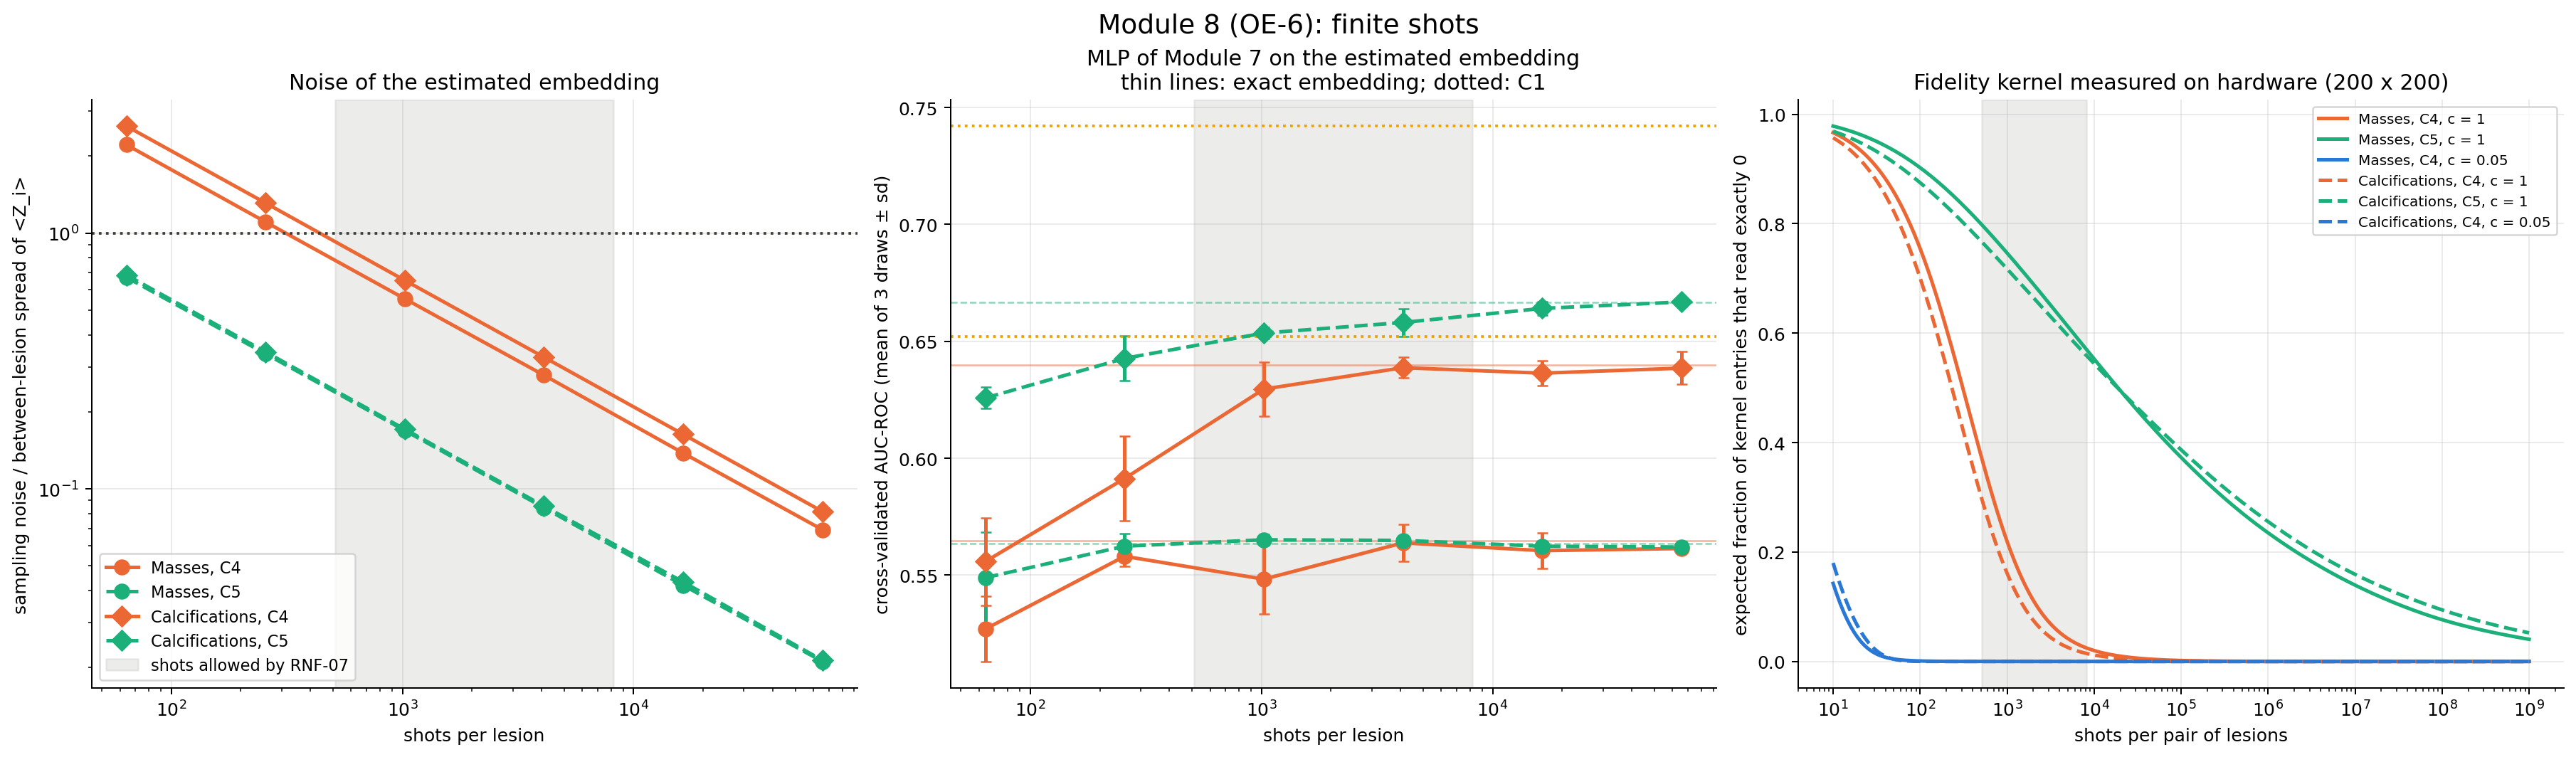
\includegraphics[width=\textwidth]{Figures/M8_oe6_shots.png}
\caption{Efecto del número de disparos (\textit{shots}) sobre la reconstrucción de expectativas en el espacio de estados y sobre la resolución empírica de matrices de kernel cuántico.}
\label{fig:m8_oe6_shots}
\end{figure}

% ---
% Hallazgos de implementación y lecciones técnicas aprendidas (OE-6).
% Sección 6.7 del reporte técnico.
% Entradas que lo respaldan: H-012, H-013, H-014, H-019, H-032, H-034, D-002, D-014, D-015, D-017, D-031.
% ---

\subsection{Hallazgos de implementación}
\label{sec:lecciones_implementacion}

La materialización práctica del pipeline experimental de aprendizaje automático cuántico en simulación clásica
condujo al descubrimiento de un conjunto de limitaciones, ambigüedades de especificación y particularidades numéricas
tanto del formalismo cuántico como de la biblioteca de desarrollo. Estos hallazgos constituyen una contribución técnica
directa a la respuesta del objetivo específico OE-6, al documentar los factores que determinan la reproducibilidad y
la viabilidad operacional del cómputo cuántico simulado. Para cada caso se distingue explícitamente entre propiedades
fundamentales del formalismo cuántico y particularidades de implementación de la biblioteca Qiskit.

% fuente: H-012, D-002; B1_benchmark_complejidad.csv
\textbf{Identidad estructural entre circuitos en mapas de Pauli.} Al comparar la fidelidad cuántica entre los
estados generados por el mapa \texttt{zz\_feature\_map} (condición C4) y el mapa general \texttt{pauli\_feature\_map}
configurado con $\text{paulis} = [\text{'Z'},\text{'ZZ'}]$ (especificación inicial de C5), se obtuvo un valor
de fidelidad idéntico a $1.000000000000$ tanto para $k = 4$ como para $k = 8$. De manera concurrente, las 18 filas del análisis
de complejidad de circuitos en B1 resultaron exactamente idénticas en profundidad cruda (50 a 112), profundidad transpilada
(58 a 126), compuertas CX (63 a 285) y conteo total de compuertas (187 a 725). Este comportamiento obedece a un
\textbf{detalle de implementación de Qiskit}: en la biblioteca, la función \texttt{zz\_feature\_map} está definida de
forma literal como una invocación a \texttt{pauli\_feature\_map} con el conjunto $[\text{'Z'},\text{'ZZ'}]$. Por tanto,
ambas opciones representaban el mismo circuito y no constituían condiciones experimentales independientes. Ante esta evidencia,
se descartó esa especificación y se evaluaron configuraciones alternativas con idéntico coste de compuertas
entrelazadoras ($n_{cx} = 12$) promediando sobre 200 entradas aleatorias en $[0, \pi]^4$.

% fuente: H-034, D-015, D-031
\textbf{Inoperancia del operador Pauli X tras la capa de Hadamard.} Al formular la condición C5 mediante
$\text{paulis} = [\text{'X'},\text{'ZZ'}]$ con el propósito de alternar el eje de rotación de primer orden,
la fidelidad respecto a un circuito que omite por completo los términos lineales en $X$ (un mapa puramente $ZZ$) arrojó
un valor mínimo de $0.99999999999999$ para 20 entradas al azar con $reps = 1$, y sobre las lesiones reales de masas la
discrepancia máxima en las matrices de kernel fue de $5.9 \times 10^{-15}$. Este fenómeno corresponde a una
\textbf{propiedad del formalismo cuántico}: la capa inicial de compuertas Hadamard prepara a cada qubit en el estado
$|+\rangle$, el cual es autoestado de la compuerta de Pauli $X$ con autovalor $+1$. La rotación $R_X(2x_i) = H P(2x_i) H$
actúa sobre su propio autoestado multiplicando al qubit únicamente por una fase compleja escalar. Sobre el estado producto
global, estas fases individuales se agregan en una fase global indetectable que no afecta ninguna medición ni producto
interno. Como consecuencia, se redefinió la condición
C5 utilizando $\text{paulis} = [\text{'Y'},\text{'ZZ'}]$, donde la rotación en $Y$ no preserva el autoestado ecuatorial
y modifica sustantivamente la codificación previa al entrelazamiento $ZZ$.

% fuente: H-013, D-014
\textbf{Nulidad idéntica del vector de expectativas sin capa variacional.} Al evaluar el vector de valores
esperados $\langle Z_i \rangle$ directamente a la salida del mapa de características $ZZ$ prescindiendo del \textit{ansatz}
variacional, el resultado fue $\langle Z_i \rangle = 0$ de forma exacta para todo qubit y cualquier vector de entrada $x$.
Este resultado responde a una \textbf{propiedad del formalismo cuántico}: partiendo del estado de superposición uniforme
$H^{\otimes k}|0\rangle$ (en el cual todas las amplitudes poseen módulo $2^{-k/2}$), todas las compuertas que componen el
mapa $ZZ$ (rotaciones de fase $R_Z$ y bloques $CX-R_Z-CX$) son operadores diagonales en la base computacional. Las matrices
diagonales multiplican cada amplitud por factores de fase compleja pero preservan de forma estricta sus magnitudes originales.
Por lo tanto, la probabilidad marginal de medir cero satisface $P(\text{qubit}_i = 0) = 1/2$, lo que impone $\langle Z_i \rangle = 0$.
Toda la información inyectada por el mapa reside en las fases relativas, respecto a las cuales la medición en $Z$ es ciega.
En respuesta, se concluyó que bajo la Arquitectura~B el \textit{ansatz} variacional es metodológicamente indispensable:
sus parámetros $\boldsymbol\theta$ deben fijarse con una semilla declarada (semilla 42) para que las rotaciones $R_Y(\boldsymbol\theta)$
proyecten las diferencias de fase a poblaciones medibles. Asimismo, se clarificó que el kernel de fidelidad no sufre esta
limitación al operar sobre los vectores de estado completos en el espacio de Hilbert.

% fuente: H-019, H-014, H-016; B3_origen_suelo_h016.csv, B3_shots_muestreo_real.csv
\textbf{Valores por defecto en estimadores y modelado de disparos en Aer.} En las evaluaciones iniciales
de sensibilidad al número de disparos (*shots*), el error frente a la supuesta referencia analítica se estancaba en un suelo
constante de $\approx 0.013$ hasta un millón de disparos, y el error parecía insensible entre 512 y 8\,192 disparos.
Este comportamiento combinó una \textbf{propiedad del formalismo cuántico} con dos \textbf{detalles de implementación de Qiskit}.
En el formalismo, la dispersión por disparos decae como $1/\sqrt{n}$ con varianza $(1 - \langle Z_i \rangle^2)/n$. En la biblioteca,
la clase \texttt{EstimatorQNN} se construye con una precisión por defecto de $0.015625$ ($= 1/\sqrt{4096}$) y sobrescribe cualquier
precisión fijada en el estimador subyacente; al transferir dicho valor a \texttt{StatevectorEstimator}, este último suma ruido
gaussiano $\mathcal{N}(0, \text{precisión})$ incluso en simulación de vector de estado, generando un error medio analítico de
$0.015625 \sqrt{2/\pi} = 0.01247$ en la referencia teórica. Además, el estimador \texttt{EstimatorV2} de Aer no simula disparos
discretos, sino que calcula la expectativa analítica y le adiciona ruido gaussiano continuo, generando una dependencia circular
con pendiente log-log de $-0.5065$. En consecuencia, se invalidó aquel hallazgo preliminar y la sección de disparos de B1; para el Módulo 5 se fijó
que toda expectativa exacta debe evaluarse con \texttt{Statevector} directo o primitivas con precisión cero explícita (\texttt{default\_precision = 0.0});
y para modelar disparos reales se adoptó en B3 el muestreador \texttt{SamplerV2} de Aer a partir de cadenas de bits y, en el estudio
del OE-6, el muestreo multinomial sobre las probabilidades exactas $|\psi(\mathbf{x})|^2$, equivalente al anterior sin ruido de
compuerta. En B3 se verificaron pendientes de $-0.4986$ en dispersión y $-0.4983$ en MAE sin suelo espurio hasta $2^{20}$ disparos.

% fuente: H-032, D-017
\textbf{Aceleración analítica mediante productos internos matriciales.} La estimación inicial de tiempo de cálculo
en B1 proyectaba aproximadamente 41 minutos por matriz de kernel cuántico de $200 \times 200$ mediante \texttt{FidelityQuantumKernel}
(superando las 2.75~h para las cuatro matrices del protocolo), mientras que la implementación con \texttt{FidelityStatevectorKernel}
evaluó la misma matriz exacta en 1.5\,s. Este hallazgo constituye un \textbf{detalle de implementación del simulador clásico}:
\texttt{FidelityQuantumKernel} construye y ejecuta circuitos cuánticos independientes de tipo \textit{compute-uncompute} por cada
par de muestras ($O(N^2)$ ejecuciones de circuito), mientras que \texttt{FidelityStatevectorKernel} aprovecha la disponibilidad
simultánea de los $N$ vectores de estado en memoria clásica ($O(N)$ simulaciones) y calcula la matriz completa mediante productos
internos vectoriales directos. Se adoptó \texttt{FidelityStatevectorKernel} para agilizar los módulos M6 y derivados en más de
tres órdenes de magnitud ($\sim 1\,000\times$), explicitando en el reporte que dicho atajo computacional es una ventaja
exclusiva de la simulación clásica que no existe en procesadores cuánticos físicos.

% fuente: D-031
\textbf{Obsolescencia de \texttt{PauliFeatureMap} en Qiskit~2.x.} A partir de Qiskit~2.1, la clase
\texttt{PauliFeatureMap} está marcada como obsoleta en favor de la función \texttt{pauli\_feature\_map()}, que devuelve un
\texttt{QuantumCircuit} estándar. Se trata de un \textbf{detalle de implementación de la API de Qiskit}, sin consecuencia
sobre el circuito que se construye. El código del proyecto emplea las funciones \texttt{pauli\_feature\_map()} y
\texttt{zz\_feature\_map()}.

% ---
% Síntesis global por objetivo específico (OE-1 a OE-6) y evaluación por dimensiones.
% Sección 6.8 del reporte técnico.
% Entradas que lo respaldan: H-001, H-005, H-020, H-023, H-024, H-026, H-035, H-038, H-039, H-040, H-041, H-042, H-043, H-049, H-051, H-052, H-032, D-012, D-014, D-016, D-031, D-036.
% ---

\subsection{Síntesis por objetivo específico}
\label{sec:sintesis_objetivos}

% fuente: H-039, H-040, H-042, H-044; 6_alineamiento_kernel.csv, 6_dimension_efectiva.csv, 6_diferencia_geometrica_resumen.csv,
% 6_metricas_embedding.csv, 7_cv_resumen.csv, 7_test.csv, X4_test.csv, 5a_resumen.csv, 5a_tiempos_clasicos.csv.
% Tabla añadida el 2026-10-20; tiempos de C2 y C3 medidos con Code/tools/tiempos_transformacion.py (5a no los cronometraba).
La Tabla~\ref{tab:resumen_resultados} reúne en un solo lugar las métricas principales de las cinco condiciones.
En la familia de kernels, el exceso de alineamiento de C4 y C5 (0.003 a 0.007) queda muy por debajo del kernel RBF
(0.049 en masas y 0.151 en calcificaciones) y su dimensión efectiva, cercana a 170--190 de 200, refleja la concentración.
El mismo MLP clasifica peor sobre C4 y C5 que sobre C1--C3, mientras que una máquina de vectores de soporte sobre
el kernel de C4 queda cerca de la que usa el kernel RBF. En costo, PCA y Kernel PCA transforman todas las lesiones
en menos de 0.2\,s, frente a 13 a 16\,s de los dos mapas cuánticos simulados con vectores de estado.

\input{tablas/resumen_resultados}

% Añadido el 2026-10-23: vista de conjunto de todas las comparaciones del trabajo, una por experimento.
La Tabla~\ref{tab:mapa_comparaciones} ordena por experimento todas las comparaciones del trabajo: qué
pregunta respondió cada una, qué se comparó, el resultado principal y su lectura. En la tarea diagnóstica,
lo clásico va por delante o, en el mejor caso para lo cuántico, empata; lo cuántico solo gana con un
etiquetado diseñado a partir de su propia geometría.

% fuente: H-039, H-042, H-043, H-035, H-044, H-047, H-053, H-054, H-056, H-050, H-048, H-057; 6_alineamiento_kernel.csv, 7_test.csv, X1_auc_por_condicion.csv, X4_test.csv, X6_test.csv, X7_resumen.csv, X8_test.csv, X10_test.csv, X11_transicion.csv, X6_etiquetas_construidas.csv
\begin{table}[htbp]
\centering
\small
\caption{Mapa de las comparaciones del trabajo. AUC-ROC en el conjunto de prueba salvo que se indique validación cruzada (VC); masas / calcificaciones. En negritas, el mejor valor de cada comparación.}
\label{tab:mapa_comparaciones}
\begin{adjustbox}{max width=\linewidth}
\begin{tabular}{p{0.1\linewidth} p{0.2\linewidth} p{0.2\linewidth} p{0.27\linewidth} p{0.17\linewidth}}
\toprule
\textbf{Exp.} & \textbf{Pregunta} & \textbf{Comparación} & \textbf{Resultado} & \textbf{Lectura} \\
\midrule
M6 (\S\ref{sec:separabilidad_representaciones}) & ¿Separan mejor las clases las representaciones cuánticas? & Métricas de kernel y de representación en C1--C5 & Exceso de KTA de 0.003 a 0.007 en C4 y C5, frente a \textbf{0.049} / \textbf{0.151} del RBF & Clásicas por delante en todas las métricas \\
M7 (\S\ref{sec:rendimiento_clasificacion}) & ¿Clasifica mejor el mismo perceptrón sobre C4 o C5? & MLP $12 \to 32 \to 16 \to 1$ en C1--C5 & C1: \textbf{0.651} / \textbf{0.769}; C4: 0.530 / 0.633; C5: 0.581 / 0.652 & Clásicas, de 0.07 a 0.14 por delante \\
M7, sensibilidad & ¿Depende de la red, la semilla, \texttt{reps} o $k$? & Semillas, redes 16-8 y 64-32, sin estandarizar, 200 épocas, \texttt{reps} = 2, $k = 8$ & La semilla mueve el AUC como mucho 0.039; la brecha se mantiene & Sin cambio \\
X1 & ¿Cuánto cuesta usar 12 de las 67 características? & Regresión logística con 67 y con 12 & \textbf{0.693} / \textbf{0.800} frente a 0.650 / 0.758 (VC) & Pérdida de 2 a 4 puntos, igual para todas las condiciones \\
X4 & ¿Se pierde la información al codificar o al leer? & QSVM de C4, SVM RBF y MLP sobre $\langle Z_i\rangle$ & 0.628 / 0.759; \textbf{0.649} / \textbf{0.769}; 0.530 / 0.633 & Empate entre QSVM y SVM; la pérdida está en la lectura \\
X6 & ¿Gana algún kernel cuántico con la misma búsqueda en ambos lados? & 28 candidatos cuánticos frente a 12 clásicos, búsqueda anidada & \textbf{0.656} frente a 0.652 / 0.755 frente a \textbf{0.760} & Empate \\
X7 & ¿Sesgó el sorteo de $\boldsymbol\theta$ el resultado? & Diez sorteos de $\boldsymbol\theta$ & Ninguno alcanza a C1; déficit de 0.03 a 0.18 (VC) & Clásicas \\
X8 & ¿Ayuda entrenar $\boldsymbol\theta$? & $\boldsymbol\theta$ entrenado frente a fijo & Gana de $+0.003$ a $+0.041$; sigue entre $-0.066$ y $-0.118$ frente a C1 & Clásicas \\
X10 & ¿Cambia con árboles o con tres \textit{folds}? & Árboles, \textit{random forest} y XGBoost en C1--C5; MLP con tres \textit{folds} & \textit{Random forest}, C1: \textbf{0.636} / \textbf{0.768}; C4: 0.591 / 0.651; C5: 0.614 / 0.624 & Clásicas; en masas, empate con los ensambles \\
M8 (\S\ref{sec:comparacion_global}) & ¿Cuánto separan los descriptores del radiólogo? & Regresión logística sobre forma y margen, o tipo y distribución & \textbf{0.872} / \textbf{0.825} (VC) & Referencia clínica, no competidor \\
X6, X11 & ¿Existe una tarea con ventaja cuántica sobre estas lesiones? & QSVM proyectado frente al mejor clásico con el etiquetado diseñado & \textbf{0.998} frente a 0.857 / \textbf{0.994} frente a 0.876 (VC); $\alpha^{*}$ de 0.4 a 0.7 & Cuántico, solo con el etiquetado diseñado \\
\bottomrule
\end{tabular}
\end{adjustbox}
\end{table}

A fin de articular los hallazgos empíricos obtenidos a lo largo del protocolo experimental con los compromisos
planteados al inicio de la investigación, la Tabla~\ref{tab:sintesis_objetivos_especificos} presenta una síntesis
estructurada por cada uno de los seis objetivos específicos (OE-1 a OE-6) formulados en el planteamiento del trabajo.
Para cada objetivo se resume el alcance establecido, la evidencia cuantitativa central generada, la sección del
reporte donde se desarrolla el análisis detallado y la respuesta concreta alcanzada en función de los datos.

% fuente: H-001, H-005, H-020, H-023, H-024, H-026, H-035, H-038, H-039, H-040, H-041, H-042, H-043, H-049, H-051, H-052, H-032, D-012, D-014, D-016, D-031, D-036; 2_preprocesamiento_qa.csv, X1_varianza_retenida.csv, B1_benchmark_arquitectura.csv, 6_alineamiento_kernel.csv, 6_dimension_efectiva.csv, 6_diferencia_geometrica_resumen.csv, 7_cv_por_fold.csv, 7_test.csv, 7_test_diferencias.csv, 8_spearman.csv, 8_oe6_qubits.csv, 8_oe6_shots_kernel.csv, 8_oe6_shots_embedding.csv, 8_oe6_resumen.csv
\begin{table}[htbp]
\centering
\small
\caption{Síntesis de resultados y evidencia empírica por objetivo específico.}
\label{tab:sintesis_objetivos_especificos}
\begin{adjustbox}{max width=\linewidth}
\begin{tabular}{p{0.07\linewidth} p{0.24\linewidth} p{0.31\linewidth} p{0.14\linewidth} p{0.24\linewidth}}
\toprule
\textbf{Objetivo} & \textbf{Objetivo resumido} & \textbf{Evidencia principal} & \textbf{Sección} & \textbf{Resultado} \\
\midrule
OE-1 & Construir pipeline sobre CBIS-DDSM (DICOM, ROI, 67 variables radiómicas, selección a $k = 12$ y escalado angular $[0, \pi]$ en subproblemas independientes). & 3\,568 registros con cobertura DICOM 100\,\%; 67 variables extraídas; 12 seleccionadas retienen 86.8\,\% (masas) y 90.2\,\% (calcificaciones) de varianza; 0 solapes entre train y test. & Sección~\ref{sec:datos_caracteristicas_seleccion} & Pipeline validado sin fuga de pacientes; selección por prueba F con filtro de redundancia ($|r| \le 0.95$) y escalado por cuantiles con IQR de $\pi/2$. \\
\midrule
OE-2 & Implementar cinco condiciones experimentales de dimensión $k = 12$ (C1 crudo, C2 PCA lineal, C3 Kernel PCA RBF, C4 ZZFeatureMap, C5 PauliFeatureMap). & 5 condiciones simétricas sobre el mismo vector; $\boldsymbol\theta$ fijo (semilla 42) en Arquitectura~B; C5 diferenciado con compuertas $Y$ y $ZZ$; extracción analítica en 0.20\,h frente a 381.7\,h estimadas en el benchmark de recursos para entrenar los dos mapas con Arquitectura~A. & Secciones~\ref{sec:modulo5}, \ref{sec:lecciones_implementacion} & Condiciones implementadas; control nulo C2 preservado; Arquitectura~B desacopla codificación de clasificación favoreciendo la reproducibilidad. \\
\midrule
OE-3 & Analizar y comparar separabilidad de clases en las cinco condiciones mediante KTA, diferencia geométrica $g$, Davies--Bouldin y razón de Fisher. & A $c = 1$, exceso de KTA de 0.003 a 0.007 en C4/C5 frente a 0.049 y 0.151 en RBF; $d_{\mathrm{eff}}$ cuántica de 167.6 a 187.7; $g$ mínima de 1.40 a 1.70 ($\sqrt{N} \approx 14.1$); condiciones clásicas superan a cuánticas en Fisher. & Sección~\ref{sec:separabilidad_representaciones} & Las transformaciones cuánticas a $c = 1$ no muestran mayor separabilidad que las clásicas en ninguna familia métrica; matrices de kernel concentradas próximas a la identidad. \\
\midrule
OE-4 & Entrenar un mismo clasificador MLP sobre las cinco representaciones bajo idéntica arquitectura, hiperparámetros y validación cruzada 5-fold por paciente. & Red $12 \to 32 \to 16 \to 1$, optimizador Adam, parada temprana; variación máxima por semilla de 0.039 en CV; 200 épocas sin parada temprana no mejora C4/C5 (AUC 0.533 y 0.557 en masas; 0.596 y 0.631 en calcificaciones). & Sección~\ref{sec:rendimiento_clasificacion} & Protocolo simétrico validado; convergencia uniforme; el déficit cuántico no es atribuible a subentrenamiento ni a sensibilidad de hiperparámetros. \\
\midrule
OE-5 & Evaluar si la separabilidad se traslada a clasificación binaria (AUC-ROC, F1, Accuracy, Precision, Recall) y correlación de Spearman entre rankings. & En test, AUC masas: C1 0.651, C3 0.646, C4 0.530, C5 0.581; calcificaciones: C1 0.769, C3 0.758, C4 0.633, C5 0.652. Diferencias frente a C1 entre $-0.07$ y $-0.14$. Coeficiente $\rho_s$ descriptivo en el rango de 0.67 a 0.97. & Secciones~\ref{sec:rendimiento_clasificacion}, \ref{sec:comparacion_global} & El MLP clasifica peor sobre C4/C5; separabilidad y clasificación coinciden en su ordenamiento (C1--C3 delante de C4--C5), pero sin ganancia previa en separabilidad que trasladar. \\
\midrule
OE-6 & Evaluar restricciones prácticas y del simulador cuántico (recursos, escalabilidad en qubits, gradientes y shots) para determinar viabilidad en salud. & Simulación exacta viable hasta $k \approx 25$ en 24\,h; gradiente por \textit{parameter-shift} requiere 5.16\,s/muestra ($\sim 205$\,h a $k = 12$); a 1\,024 disparos, entre 15.7\,\% y 74.5\,\% de pares del kernel leen cero; MLP tolera disparos perdiendo $< 0.02$ de AUC. & Secciones~\ref{sec:restricciones_simulador}, \ref{sec:lecciones_implementacion} & Techo práctico impuesto por gradientes físicos y concentración del kernel; fidelidad experimentalmente inmedible con disparos realistas en NISQ; atajos de simulación no trasladables a hardware. \\
\bottomrule
\end{tabular}
\end{adjustbox}
\end{table}

A partir de esta correspondencia empírica, la respuesta integral a la pregunta de investigación se estructura
en torno a las tres dimensiones de análisis que fundamentaron el planteamiento del problema:

% fuente: H-038, H-039, H-040, H-041; 6_alineamiento_kernel.csv, 6_dimension_efectiva.csv, 6_diferencia_geometrica_resumen.csv
\textbf{Dimensión de representación (OE-3).} Respecto a la capacidad de las transformaciones cuánticas
variacionales para generar espacios de características con mayor separabilidad de clases, la evidencia empírica
indica de forma consistente que los mapas cuánticos evaluados a escala nominal ($c = 1$) no superan a las
representaciones clásicas de referencia en ninguna de las familias métricas analizadas. En el espacio de kernels,
el exceso de alineamiento centrado (\textit{kernel-target alignment}, KTA) de C4 y C5 se sitúa entre 0.003 y 0.007,
abarcando menos del 10\,\% del exceso registrado por el kernel gaussiano RBF clásico (0.049 en masas y 0.151 en
calcificaciones); las matrices cuánticas resultan cercanas a la identidad con una dimensión efectiva que satura
el espacio disponible ($d_{\mathrm{eff}} \approx 168$--$188$ sobre 200), y la diferencia geométrica regularizada
($g \approx 1.40$--$1.70$) permanece muy alejada de la cota teórica de ventaja cuántica potencial ($\sqrt{N} \approx 14.1$).
Asimismo, en las representaciones locales $\langle Z_i \rangle$, los índices de Fisher y Davies--Bouldin sitúan a
las condiciones clásicas C1 y C3 sistemáticamente por delante de las condiciones cuánticas. Aunque la contracción
angular ($c \to 0.02$) o la reducción a 8 qubits (X3) atenúan la concentración, dicha recuperación no introduce
estructura cuántica genuina: el alineamiento solo se aproxima al clásico en el régimen en que el producto cruzado
entre características deja de influir, emulando la geometría de un kernel clásico.

% fuente: H-042, H-043, H-049; 7_test.csv, 7_test_diferencias.csv, 8_spearman.csv
\textbf{Dimensión de clasificación (OE-5).} En lo concerniente a si la transformación cuántica se traduce en una
mejora en la clasificación binaria de lesiones mamográficas, los resultados sobre el clasificador perceptrón multicapa
muestran que el mismo modelo clasifica de manera desfavorable sobre las representaciones cuánticas C4 y C5 en comparación
con las condiciones clásicas. En el conjunto de prueba independiente, las condiciones cuánticas exhiben un déficit de
0.07 a 0.14 de AUC-ROC frente al vector de características crudas C1 (alcanzando 0.530 en C4 masas y 0.633 en C4 calcificaciones,
frente a 0.651 y 0.769 en C1), brecha estadísticamente significativa respaldada por intervalos de confianza por remuestreo
que excluyen el cero. Este menoscabo no responde a artefactos de optimización, pues los análisis de sensibilidad sugieren
que ni la variación de semillas, ni arquitecturas alternativas, ni el entrenamiento prolongado a 200 épocas sin parada temprana
logran revertir la diferencia. El análisis de correlación de rangos de Spearman ($\rho_s \in [0.67, 0.97]$) muestra una coincidencia
descriptiva en el ordenamiento relativo de ambas etapas (con el bloque clásico C1--C3 situado por delante de C4 y C5); no obstante, debido a que
las condiciones cuánticas no alcanzaron mayor separabilidad en OE-3, no existió una ganancia representacional que pudiera
trasladarse al desempeño diagnóstico.

% fuente: H-051, H-052, H-054, H-019, H-032; 8_oe6_qubits.csv, 8_oe6_shots_kernel.csv, 8_oe6_resumen.csv, X8_costo_gradiente.csv
\textbf{Dimensión de viabilidad práctica (OE-6).} En relación con la factibilidad computacional y operacional de trasladar
estos esquemas a un contexto clínico real, las mediciones revelan restricciones fundamentales impuestas por el formalismo
físico de la medición cuántica. Si bien el clasificador de red neuronal tolera el ruido estocástico inducido por un régimen
realista de 1\,024 disparos por muestra sobre las expectativas locales $\langle Z_i \rangle$ (reteniendo el AUC exacto a menos
de 0.02), la estimación de matrices de kernel de fidelidad en procesadores cuánticos físicos resulta experimentalmente inviable
a escala nominal ($c = 1$): debido a la concentración exponencial de la fidelidad cuántica, entre el 15.7\,\% y el 74.5\,\%
de los pares de lesiones registrarían lecturas idénticamente nulas a 1\,024 disparos, y acotar el error relativo al 10\,\% exigiría una mediana de decenas de miles de
mediciones por par en C4 y de millones en C5. Asimismo, el coste computacional del gradiente exacto por \textit{parameter-shift}
(5.16\,s por muestra a $k = 12$, equivalente a unas 205~h de cálculo para 50 épocas) restringe de forma severa el entrenamiento
variacional en ausencia de los atajos de vector de estado analítico, los cuales solo existen en simulación clásica y son
inaplicables en dispositivos cuánticos físicos.

\newpage

% ===== Capítulo: A_Anexos
% ============================================================
% ANEXOS DEL REPORTE TÉCNICO
% Apertura formal del entorno de apéndices.
% ============================================================

\appendix

% Fallback para compilación aislada de A_Anexos sin 4_EDA
\makeatletter
\ifcsname r@sec:eda\endcsname\else
  \expandafter\gdef\csname r@sec:eda\endcsname{{4}{1}}
\fi
\makeatother

% ============================================================
% ANEXO A · CÓDIGO DE LOS MÓDULOS
% Fragmentos representativos de la implementación en notebooks.
% Decisiones que lo respaldan: D-008, D-014, D-017, D-018, D-020,
% D-021, D-022, D-023, D-024, D-025, D-026, D-027, D-031, D-032,
% D-033, D-036, D-039, D-040.
% ============================================================

\section{Código de los módulos}\label{anx:codigo}

En este anexo se presentan los fragmentos de código más representativos del pipeline
experimental desarrollado en el proyecto. Todos los listados incluidos han sido extraídos
de manera literal directamente desde las celdas ejecutadas de los cuadernos de trabajo
(\textit{Jupyter notebooks}) mediante la herramienta automatizada del repositorio.
Las rutinas auxiliares de utilidad general localizadas en el módulo \texttt{Code/tools/}
son omitidas en los listados para centrar la atención en la lógica nuclear de cada etapa.

% ------------------------------------------------------------
\subsection{Módulo 2: Preprocesamiento y alineación de máscaras}\label{sec:anx_m2}

% fuente: D-020
La función \texttt{align\_mask} implementa la regla de corrección espacial para las 80
máscaras del CBIS-DDSM cuyas dimensiones difieren de la mamografía completa. Cuando el
desajuste se debe a un factor de submuestreo de 0.870 se aplica interpolación al vecino
más cercano, mientras que en discrepancias de resolución nativa se preserva el anclaje
en la esquina superior izquierda sin remuestreo continuo.

\lstinputlisting[style=tt, caption={[Función de alineación espacial de máscaras]Función de alineación espacial de máscaras (\texttt{Code/2\_Preprocessing.ipynb}, celda de código 5).}, label={lst:m2_alineacion}]{codigo/m2_alineacion.py}

% fuente: D-021
La rutina \texttt{prepare\_mask} realiza el análisis morfológico de componentes conexas
mediante la función \texttt{connectedComponentsWithStats} de OpenCV. Identifica la componente de mayor área
como la lesión patológica principal y descarta motas satélite aisladas, registrando la
distancia euclidiana máxima y el número de píxeles eliminados para control de calidad.

\lstinputlisting[style=tt, caption={[Depuración y selección de componente conexa mayor]Depuración y selección de componente conexa mayor (\texttt{Code/2\_Preprocessing.ipynb}, celda de código 11).}, label={lst:m2_componente}]{codigo/m2_componente.py}

% fuente: D-022
La función \texttt{export\_mammogram} formaliza el contrato de salida del Módulo 2. Calcula
la caja delimitadora ajustada a la lesión depurada y le agrega un margen de seguridad de 20
píxeles por lado, extrayendo los parches sobre las intensidades crudas de 16 bits y
almacenándolos en formato comprimido NRRD con espaciado espacial unitario.

\lstinputlisting[style=tt, caption={[Recorte de región de interés con margen y exportación]Recorte de región de interés con margen y exportación (\texttt{Code/2\_Preprocessing.ipynb}, celda de código 13).}, label={lst:m2_recorte}]{codigo/m2_recorte.py}

% ------------------------------------------------------------
\subsection{Módulo 3: Extracción de características radiómicas}\label{sec:anx_m3}

% fuente: D-008, D-023
La inicialización del extractor radiómico fija el parámetro \texttt{binCount=32} sobre las
intensidades originales, asegurando invarianza a traslaciones lineales sin forzar un ancho
fijo de contenedor. Se inhabilitan los filtros derivados complejos y se activan únicamente
las cuatro familias morfológicas y texturales bidimensionales primarias (\textit{firstorder},
\textit{shape2D}, \textit{glcm} y \textit{glrlm}), totalizando 67 características.

\lstinputlisting[style=tt, caption={[Configuración del extractor PyRadiomics y activación de familias]Configuración del extractor PyRadiomics y activación de familias (\texttt{Code/3\_Feature\_Extraction.ipynb}, celda de código 3).}, label={lst:m3_extractor}]{codigo/m3_configuracion.py}

% ------------------------------------------------------------
\subsection{Módulo 4: Selección y escalado angular}\label{sec:anx_m4}

% fuente: D-024
La función \texttt{select} aplica un procedimiento voraz guiado por el estadístico $F$ del
análisis de varianza univariado, calculado estrictamente sobre los datos de entrenamiento.
Cada variable candidata se incorpora solo si el valor absoluto de su correlación de Pearson
frente a las variables ya seleccionadas no excede el límite de redundancia $|r| \le 0.95$.

\lstinputlisting[style=tt, caption={[Selección voraz por $F$-test con restricción de redundancia lineal]Selección voraz por $F$-test con restricción de redundancia lineal (\texttt{Code/4\_Selection\_and\_Scaling.ipynb}, celda de código 5).}, label={lst:m4_seleccion}]{codigo/m4_seleccion.py}

% fuente: D-025
El escalado angular utiliza \texttt{QuantileTransformer} configurado para proyectar a una
distribución uniforme y multiplicado por $\pi$. Esto asegura que cada característica ocupe
de forma homogénea el intervalo angular $[0, \pi]$, mitigando la influencia de asimetrías
y valores atípicos sin alterar el orden relativo de las observaciones de entrenamiento.

\lstinputlisting[style=tt, caption={[Transformación angular por cuantiles acotada a {$[0, \pi]$}]Transformación angular por cuantiles acotada a {$[0, \pi]$} (\texttt{Code/4\_Selection\_and\_Scaling.ipynb}, celda de código 8).}, label={lst:m4_escalado}]{codigo/m4_escalado.py}

% fuente: D-018, D-026
La conformación de los pliegues de validación cruzada utiliza \texttt{StratifiedGroupKFold}
para agrupar las lesiones por paciente. La rutina evalúa múltiples semillas deterministas y
selecciona aquella que minimiza la desviación máxima en la proporción de malignidad entre los
cinco pliegues, garantizando particiones homogéneas e independientes a nivel de sujeto.

\lstinputlisting[style=tt, caption={[Generación y balanceo de folds agrupados por paciente]Generación y balanceo de folds agrupados por paciente (\texttt{Code/4\_Selection\_and\_Scaling.ipynb}, celda de código 9).}, label={lst:m4_folds}]{codigo/m4_folds.py}

% ------------------------------------------------------------
\subsection{Módulo 5: Transformaciones cuánticas y kernels}\label{sec:anx_m5}

% fuente: D-014, D-031
El cálculo del embedding cuántico combina los circuitos de codificación C4 y C5 con un
\textit{ansatz} variacional \texttt{RealAmplitudes} parametrizado mediante un vector $\theta$
fijo generado con semilla 42. El valor esperado local $\langle Z_i \rangle$ se obtiene de forma
exacta multiplicando la distribución de probabilidades del vector de estado por la matriz de signos.

\lstinputlisting[style=tt, caption={[Construcción de mapas cuánticos, ansatz con $\theta$ fijo y cálculo de $\langle Z_i \rangle$]Construcción de mapas cuánticos, ansatz con $\theta$ fijo y cálculo de $\langle Z_i \rangle$ (\texttt{Code/5a\_Embeddings.ipynb}, celda de código 2).}, label={lst:m5_embeddings}]{codigo/m5_embeddings.py}

% fuente: D-017, D-027
La computación de matrices de kernel emplea \texttt{FidelityStatevectorKernel} sobre los
vectores cuánticos precomputados, optimizando el cálculo de productos internos exactos en
la submuestra representativa. En paralelo, se construye el kernel clásico RBF empleando el
ancho de banda óptimo determinado por la heurística de la mediana.

\lstinputlisting[style=tt, caption={[Evaluación de matrices de kernel clásico y cuántico]Evaluación de matrices de kernel clásico y cuántico (\texttt{Code/5b\_Quantum\_Kernels.ipynb}, celda de código 4).}, label={lst:m5_kernels}]{codigo/m5_kernels.py}

% ------------------------------------------------------------
\subsection{Módulo 6: Separabilidad geométrica}\label{sec:anx_m6}

% fuente: D-033
El alineamiento de matrices de kernel evalúa la correspondencia con la estructura de clases.
La rutina \texttt{alignment\_with\_null} centra la matriz de kernel y calcula tanto la
métrica empírica observada como su exceso respecto a la media de una distribución nula
obtenida mediante permutaciones exhaustivas de las etiquetas binarias.

\lstinputlisting[style=tt, caption={[Centrado matricial y alineamiento kernel-objetivo con prueba de permutación]Centrado matricial y alineamiento kernel-objetivo con prueba de permutación (\texttt{Code/6\_Separability.ipynb}, celda de código 3).}, label={lst:m6_kta}]{codigo/m6_kta_permutaciones.py}

% fuente: D-017, D-032
La evaluación de ventaja cuántica potencial implementa la diferencia geométrica regularizada
$g(K_C \parallel K_Q)$ descrita por Huang et al. El algoritmo computa la raíz simétrica
de la matriz cuántica y diagonaliza el kernel clásico, evaluando las cotas teóricas de
generalización y entrenamiento sobre una grilla de parámetros de regularización $\lambda$.

\lstinputlisting[style=tt, caption={[Cálculo de la diferencia geométrica regularizada de Huang et al]Cálculo de la diferencia geométrica regularizada de Huang et al. (\texttt{Code/6\_Separability.ipynb}, celda de código 3).}, label={lst:m6_geometric_difference}]{codigo/m6_geometric_difference.py}

% ------------------------------------------------------------
\subsection{Módulo 7: Clasificación supervisada}\label{sec:anx_m7}

% fuente: D-036
El clasificador neuronal común consiste en un perceptrón multicapa implementado en PyTorch
con estructura $k \to 32 \to 16 \to 1$, capas lineales continuas con activaciones ReLU y
salida en escala logit, lo que permite integrar numéricamente la función sigmoide dentro de la
función de costo de entropía cruzada binaria ponderada.

\lstinputlisting[style=tt, caption={[Definición del perceptrón multicapa para clasificación supervisada]Definición del perceptrón multicapa para clasificación supervisada (\texttt{Code/7\_Classification.ipynb}, celda de código 3).}, label={lst:m7_mlp}]{codigo/m7_mlp.py}

% fuente: D-036
El ciclo de optimización \texttt{fit\_predict} utiliza el optimizador Adam y aplica parada
temprana monitoreando la pérdida ponderada sobre una partición interna independiente de
pacientes. Si tras 40 épocas no se detecta mejoría, se detiene el entrenamiento y se
restauran los mejores pesos obtenidos para evaluar el conjunto de prueba.

\lstinputlisting[style=tt, caption={[Bucle de entrenamiento con parada temprana y restauración de pesos]Bucle de entrenamiento con parada temprana y restauración de pesos (\texttt{Code/7\_Classification.ipynb}, celda de código 3).}, label={lst:m7_parada_temprana}]{codigo/m7_parada_temprana.py}

% ------------------------------------------------------------
\subsection{Módulo 8: Evaluación comparativa y muestreo}\label{sec:anx_m8}

% fuente: D-039
El análisis comparativo evalúa la correlación de rangos de Spearman entre las métricas de
separabilidad geométrica y el desempeño clasificador. La rutina asigna rangos promedio a
condiciones empatadas y deriva la distribución nula exacta mediante las 120 permutaciones
posibles para determinar la significación estadística bilateral.

\lstinputlisting[style=tt, caption={[Cálculo del coeficiente de Spearman con empates y distribución nula exacta]Cálculo del coeficiente de Spearman con empates y distribución nula exacta (\texttt{Code/8\_Comparison.ipynb}, celda de código 6).}, label={lst:m8_spearman}]{codigo/m8_spearman.py}

% fuente: D-040
La cuantificación del coste por mediciones finitas simula el comportamiento de un dispositivo
físico mediante muestreo multinomial de las probabilidades exactas. Este procedimiento emula
un ejecutor ideal de disparos finitos (\textit{shots}) y permite contrastar el error empírico
frente a la cota teórica de desviación estándar de la medición cuántica.

\lstinputlisting[style=tt, caption={[Muestreo multinomial de mediciones finitas y ley de dispersión]Muestreo multinomial de mediciones finitas y ley de dispersión (\texttt{Code/8\_Comparison.ipynb}, celda de código 17).}, label={lst:m8_muestreo}]{codigo/m8_muestreo.py}

% ============================================================
% ANEXO B · SALIDAS Y RESULTADOS COMPLEMENTARIOS
% Tablas generadas automáticamente a partir de los datos en Code/results/.
% ============================================================

\section{Salidas y resultados complementarios}\label{anx:salidas}

En este anexo se presentan las tablas cuantitativas complementarias que respaldan las
etapas de preprocesamiento, selección de variables, validación cruzada, coste computacional
y verificación de consistencia interna del sistema. Todas las tablas han sido generadas
directamente a partir de los registros estructurados en archivos CSV del repositorio
mediante el script \texttt{tablas\_anexos.py} de \texttt{Code/tools/}, garantizando trazabilidad completa.

% ------------------------------------------------------------
\subsection{Preprocesamiento y auditoría de máscaras (Módulo 2)}

La Tabla~\ref{tab:anexo_m2_resumen} sintetiza el control de calidad aplicado sobre las 3\,568
mamografías, documentando los casos con desajuste dimensional corregidos y la concordancia con
los recortes oficiales.

\input{tablas/anexo_b_m2_resumen}

% ------------------------------------------------------------
\subsection{Selección y redundancia de características (Módulo 4)}

La Tabla~\ref{tab:anexo_m4_seleccion} reporta las 12 características radiómicas seleccionadas
en cada subconjunto clínico, acompañadas de sus estadísticos univariados de significación y tamaño del efecto.

\input{tablas/anexo_b_m4_seleccion}

La Tabla~\ref{tab:anexo_m4_redundancia} documenta las características candidatas que, a pesar de su
relevancia individual, fueron descartadas del conjunto final por exceder el límite de redundancia lineal.

\input{tablas/anexo_b_m4_redundancia}

% ------------------------------------------------------------
\subsection{Estratificación de pliegues en validación cruzada (Módulo 4)}

La Tabla~\ref{tab:anexo_m4_folds} detalla el reparto de lesiones, el número de pacientes únicos y
la proporción de malignidad en cada uno de los cinco pliegues de validación cruzada generados.

\input{tablas/anexo_b_m4_folds}

% ------------------------------------------------------------
\subsection{Costes computacionales de simulación cuántica (Módulos 5, 8 y X8)}

La Tabla~\ref{tab:anexo_m5_tiempos} presenta la comparativa de tiempos de ejecución empíricos entre
el cálculo matricial por vector de estado y la simulación individual por circuito.

\input{tablas/anexo_b_m5_tiempos}

La Tabla~\ref{tab:anexo_m8_oe6_qubits} reporta el escalamiento de los requerimientos de memoria y tiempo
de simulación en función del número de qubits del sistema, contrastando mediciones directas y extrapolaciones.

\input{tablas/anexo_b_m8_oe6_qubits}

La Tabla~\ref{tab:anexo_x8_gradiente} expone la evaluación comparativa del coste por muestra para el
cálculo de gradientes cuánticos mediante la regla analítica de desplazamiento de parámetros frente a diferenciación automática.

\input{tablas/anexo_b_x8_gradiente}

% ------------------------------------------------------------
\subsection{Verificaciones automáticas y control metodológico (Módulos 5 a 8 y X5)}

La Tabla~\ref{tab:anexo_verificaciones} resume el catálogo de verificaciones automáticas integradas
en los módulos de transformación, separabilidad y clasificación supervisada.

\input{tablas/anexo_b_verificaciones}

La Tabla~\ref{tab:anexo_x5_auditoria} reúne los resultados de la auditoría independiente de consistencia
metodológica, verificando la ausencia de fugas de datos y la integridad de las etiquetas clínicas.

\input{tablas/anexo_b_x5_auditoria}

% ============================================================
% ANEXO C · FIGURAS COMPLEMENTARIAS
% Figuras metodológicas y experimentales que complementan el cuerpo del reporte.
% Decisiones y hallazgos que las respaldan: H-016, H-018, H-019, H-020,
% H-036, H-041, H-044, H-049, D-014, D-022, D-031.
% ============================================================

\section{Figuras complementarias}\label{anx:figuras}

En esta sección se compilan aquellas figuras generadas durante las fases de caracterización,
evaluación de complejidad y análisis exploratorio del pipeline que, por razones de espacio y
fluidez narrativa, no fueron incluidas en los capítulos metodológicos ni de resultados principales.
Las figuras relativas a la distribución exploratoria de variables clínicas e imágenes DICOM
del conjunto de datos se presentan en el anexo correspondiente.

% ------------------------------------------------------------
\subsection{Preprocesamiento e imágenes de entrada}

\begin{figure}[H]
\centering
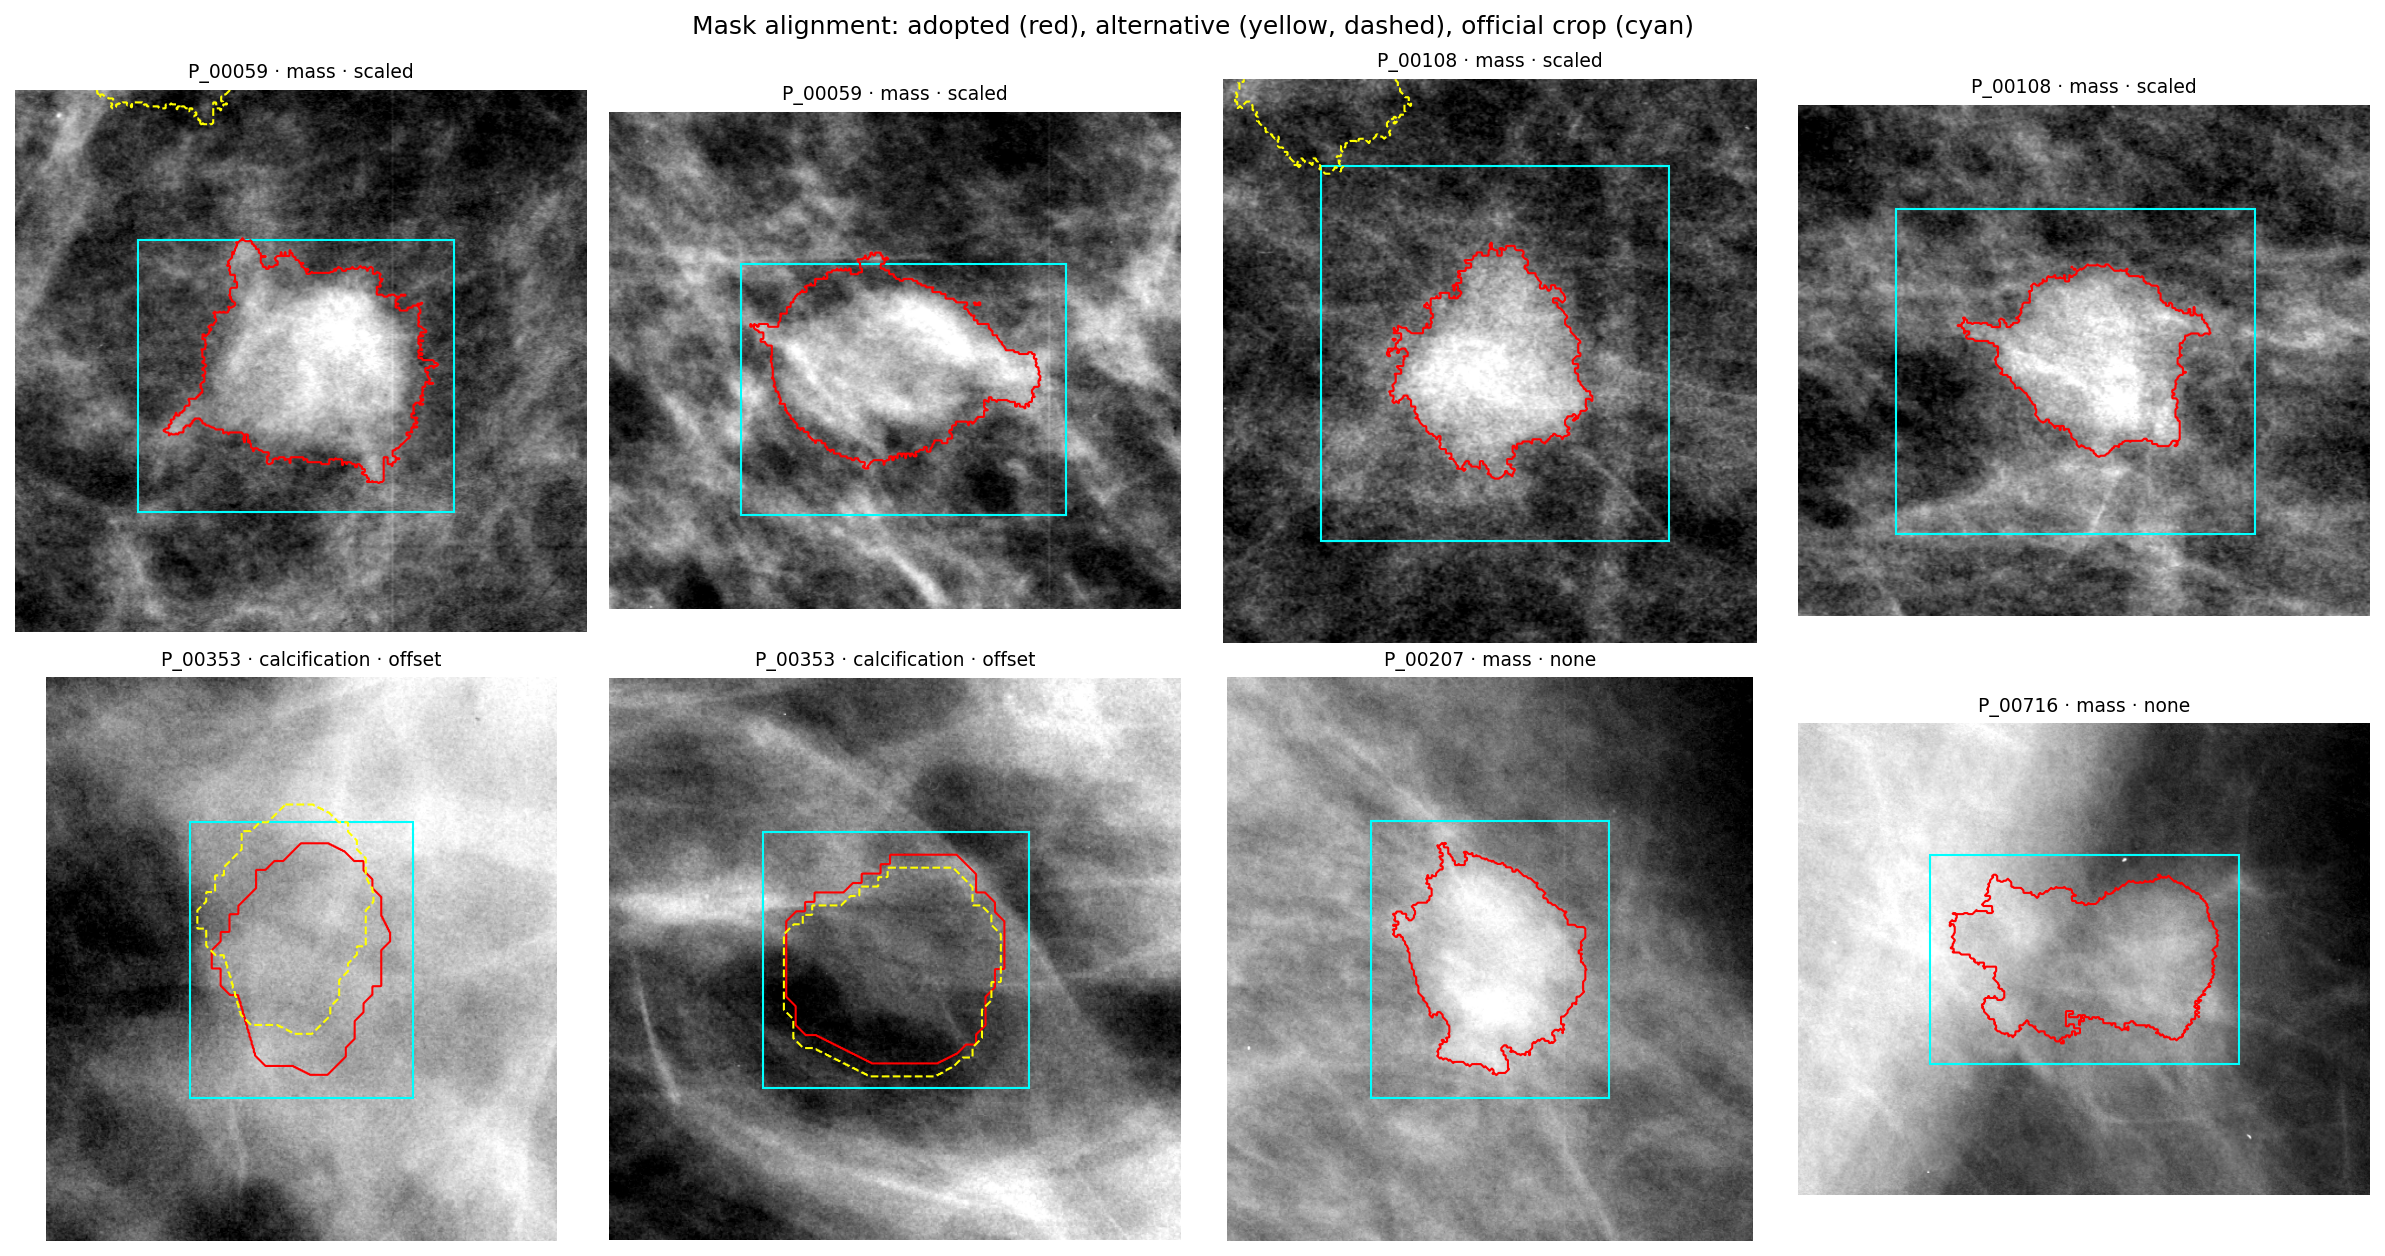
\includegraphics[width=\textwidth]{Figures/M2_mask_alignment.png}
% fuente: H-020
\caption{Diagnóstico de desajuste dimensional y verificación de alineación espacial de máscaras en el Módulo 2. Se ilustran los dos casos identificados: discordancia por factor de escala ($0.870$) y desajuste por traslación de origen, contrastados con el recorte oficial.}
\label{fig:anx_m2_alignment}
\end{figure}

\begin{figure}[H]
\centering
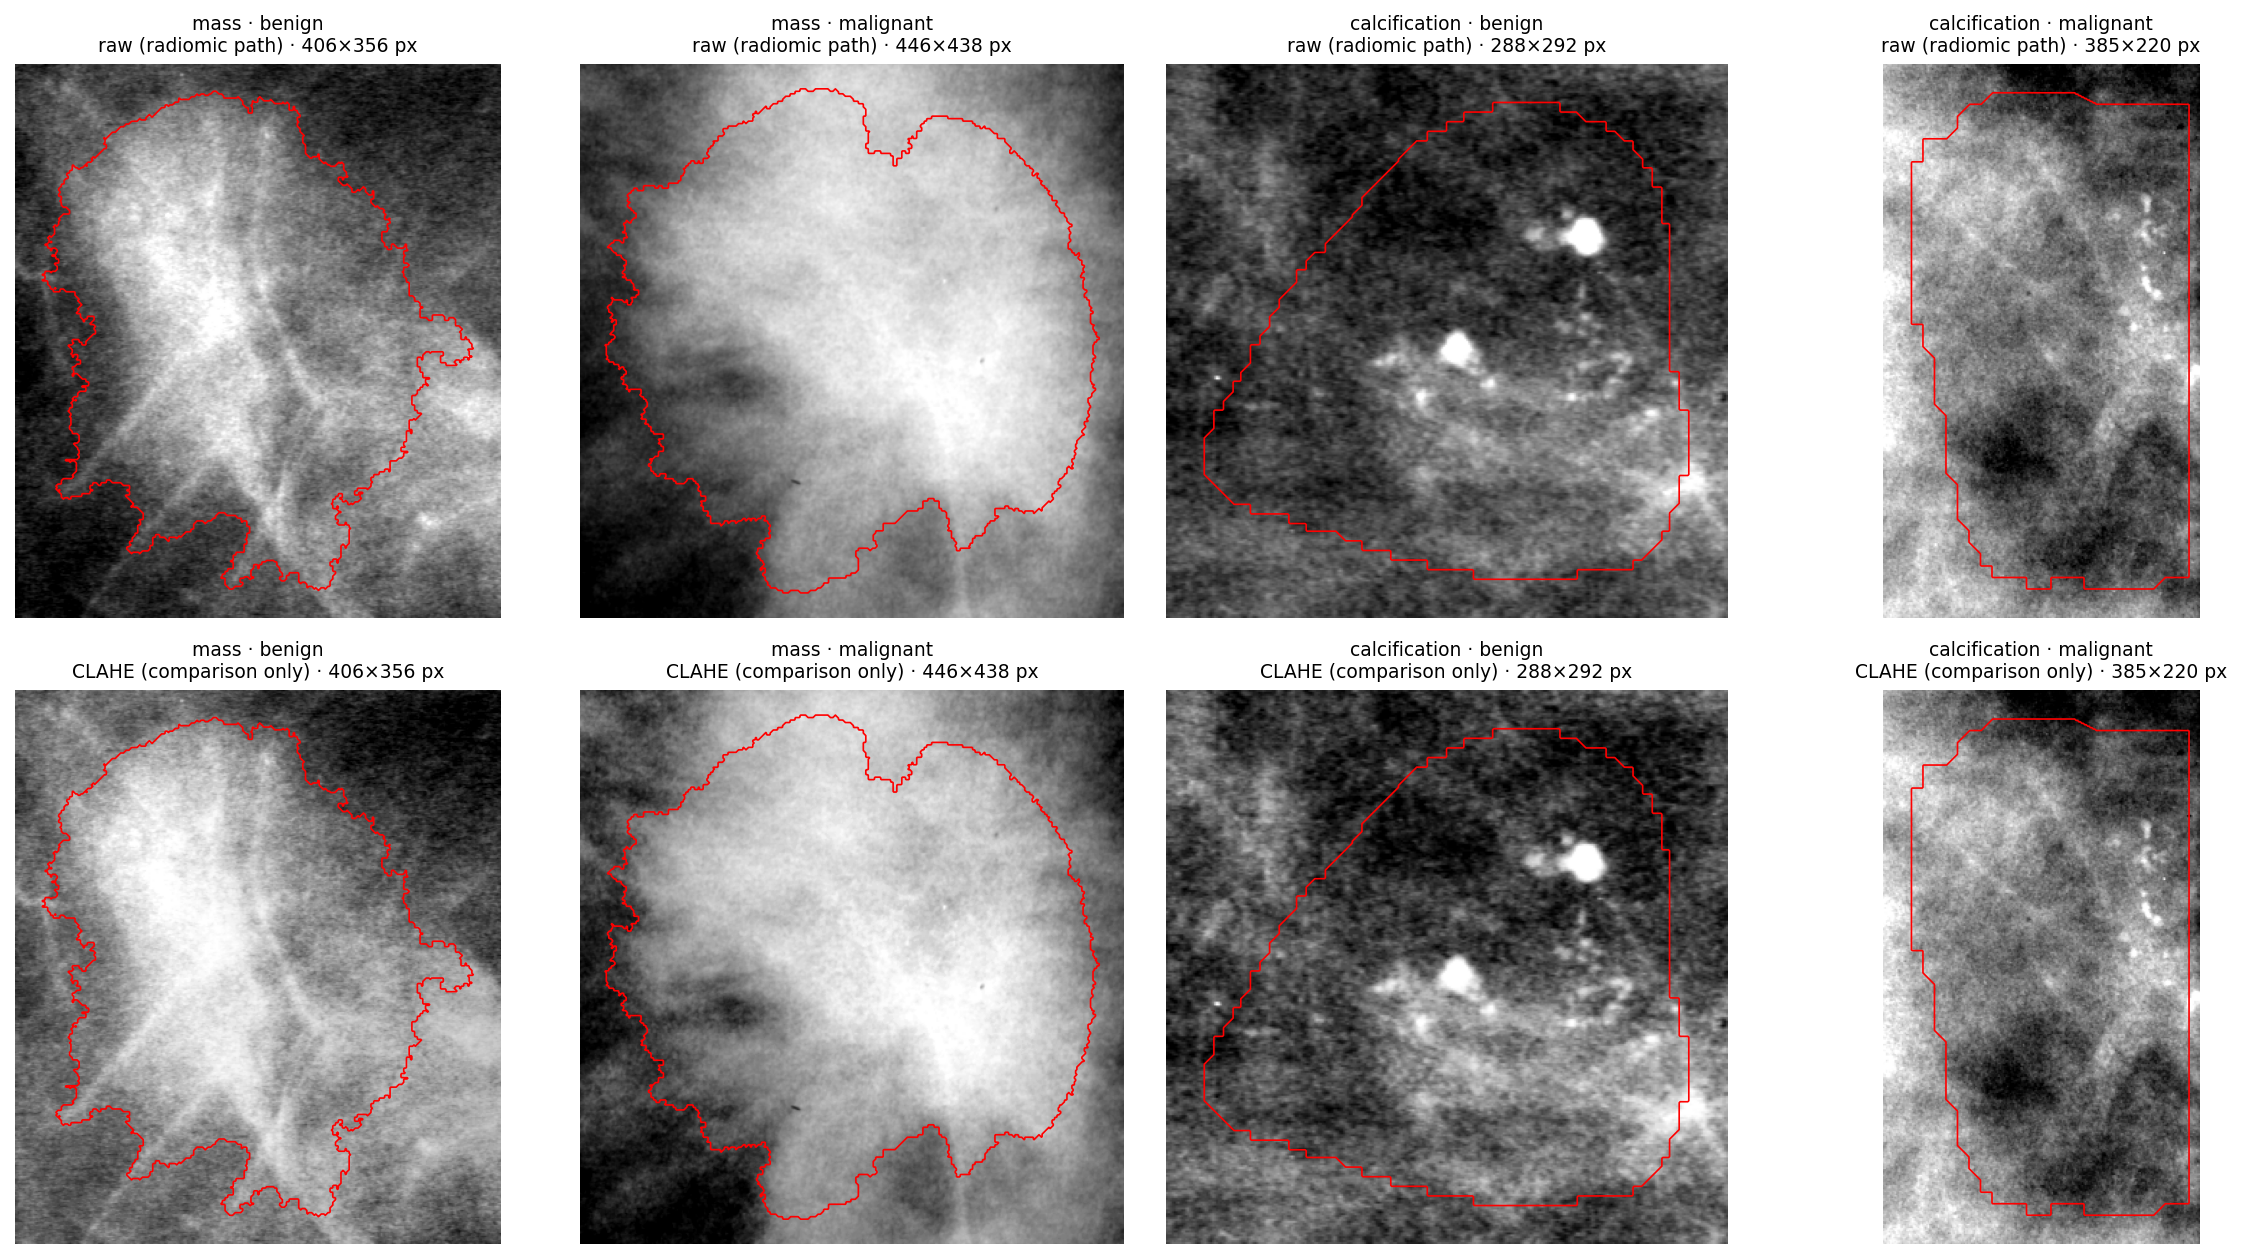
\includegraphics[width=\textwidth]{Figures/M2_preprocessing_examples.png}
% fuente: D-022
\caption{Ejemplos ilustrativos de las etapas de preprocesamiento sobre mamografías del CBIS-DDSM (Módulo 2). Se muestra la mamografía completa, la máscara binarizada depurada, la región de interés recortada con margen de seguridad y su correspondiente versión procesada mediante ecualización CLAHE.}
\label{fig:anx_m2_examples}
\end{figure}

% ------------------------------------------------------------
\subsection{Circuitos cuánticos y mapas de características}

\begin{figure}[H]
\centering
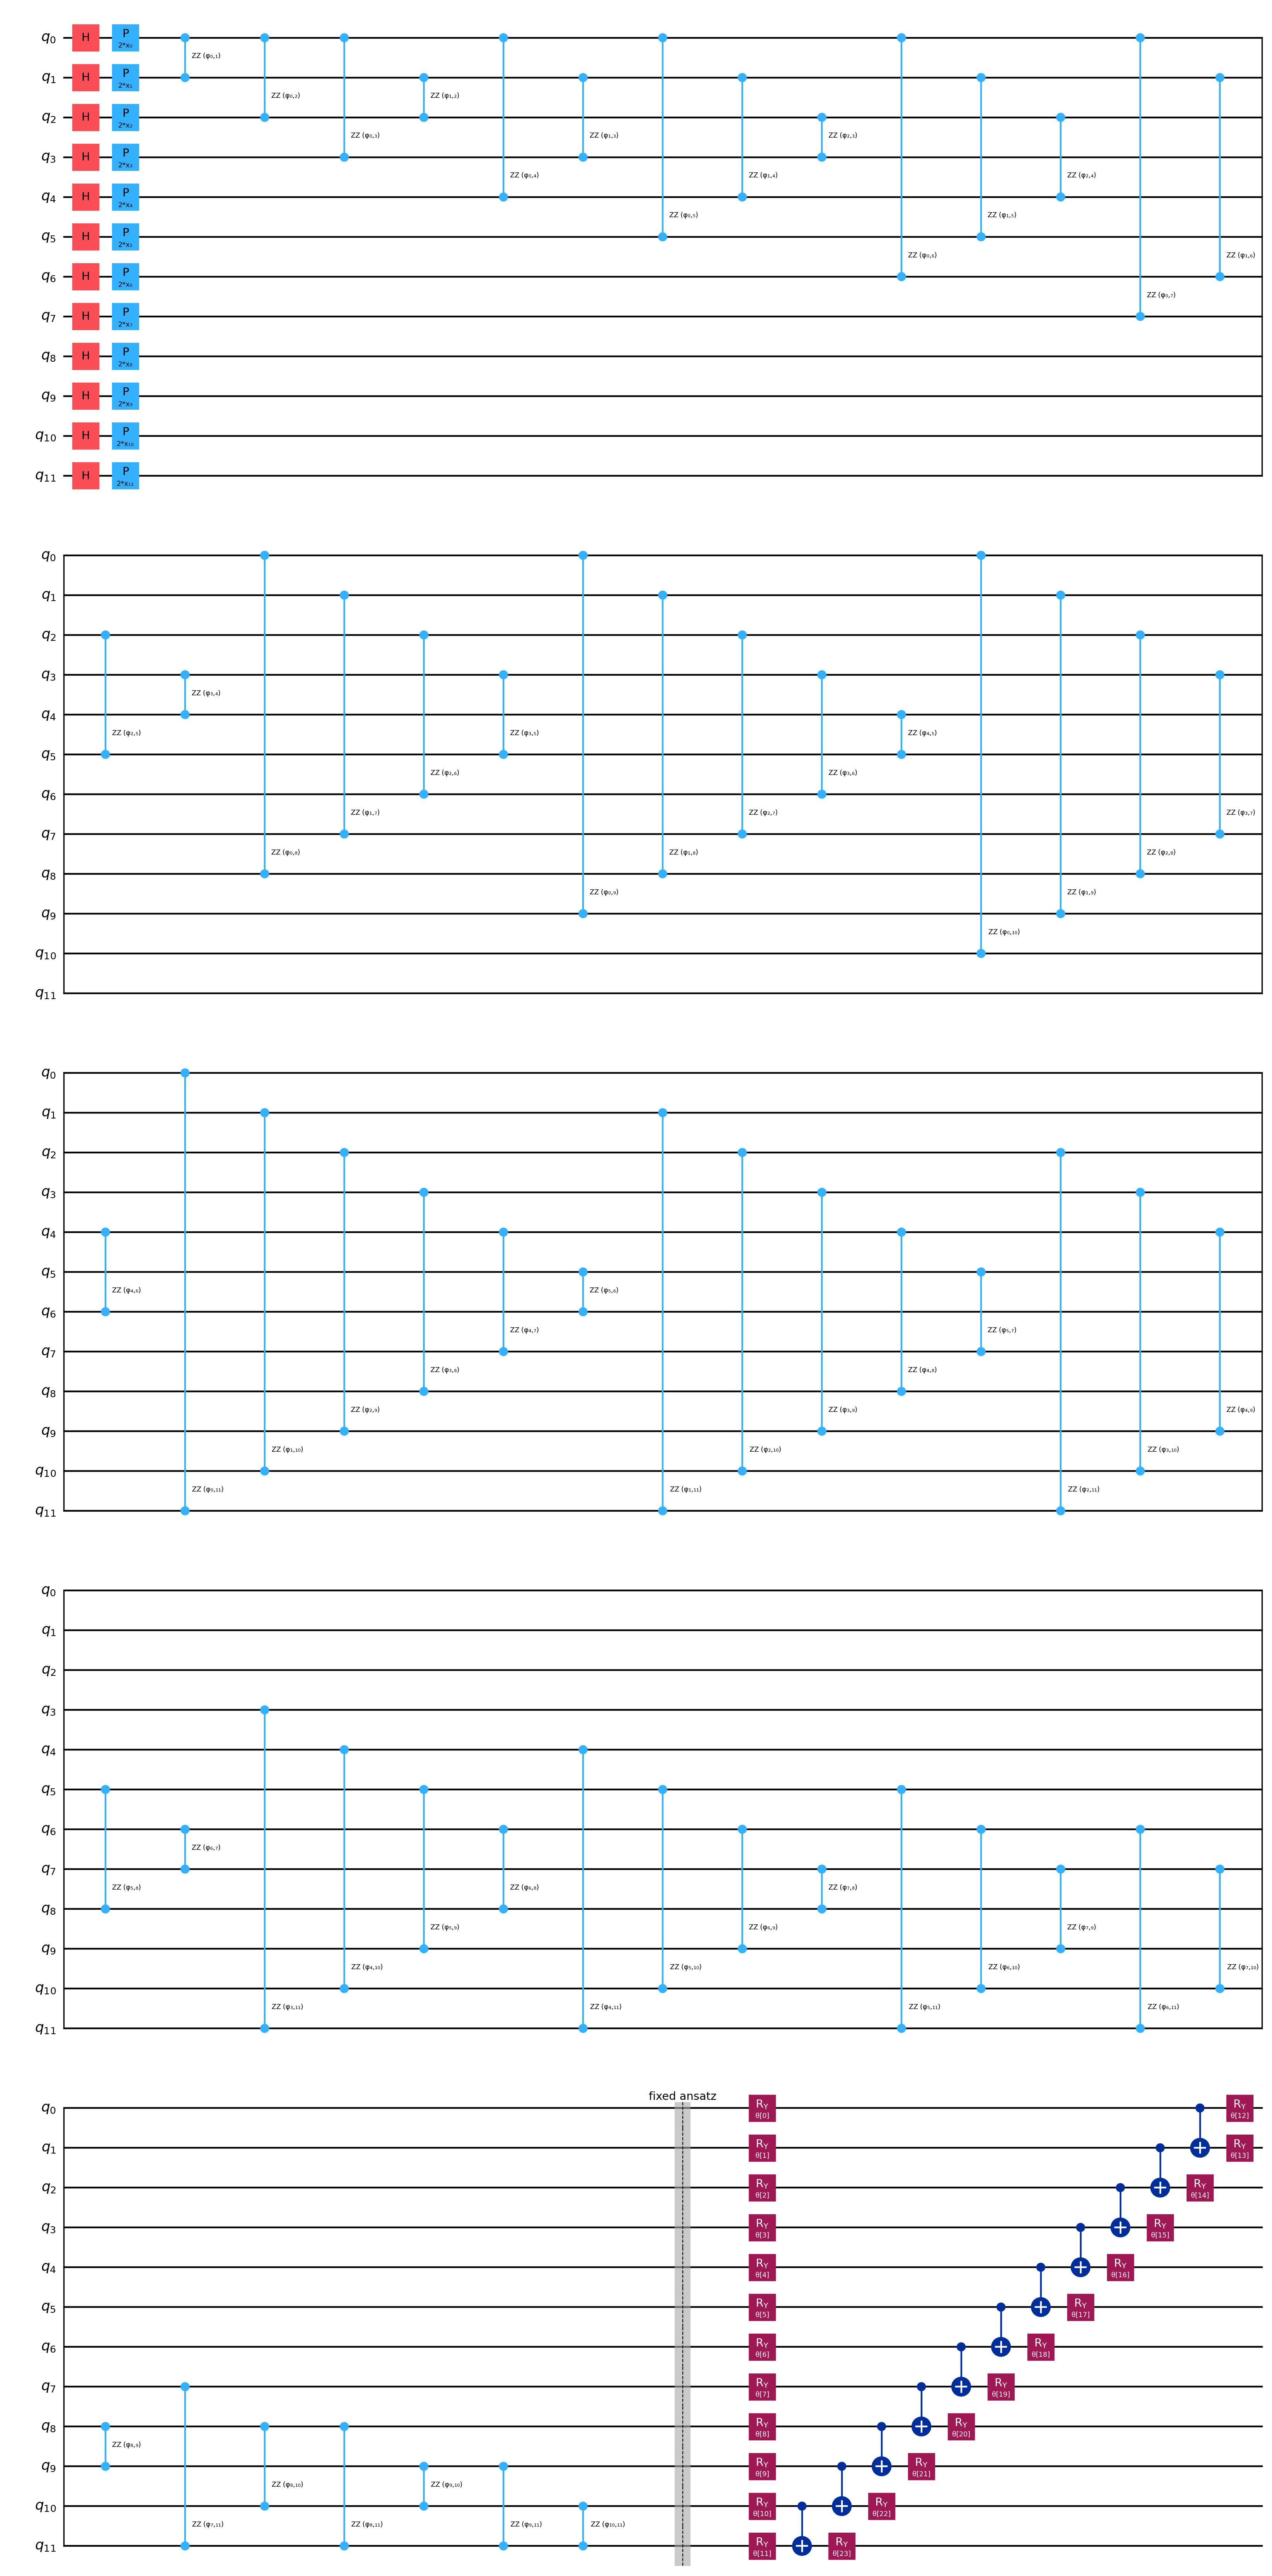
\includegraphics[width=0.6\textwidth]{Figures/M5_circuit_12q.png}
% fuente: D-031
\caption{Diagrama esquemático completo del circuito cuántico variacional implementado para $k = 12$ qubits (Módulo 5). Incluye la codificación angular de características, el entrelazamiento completo de dos qubits y la capa variacional con \textit{ansatz} \texttt{RealAmplitudes} de una repetición parametrizada con vector $\theta$ fijo.}
\label{fig:anx_m5_circuit_12q}
\end{figure}

\begin{figure}[H]
\centering
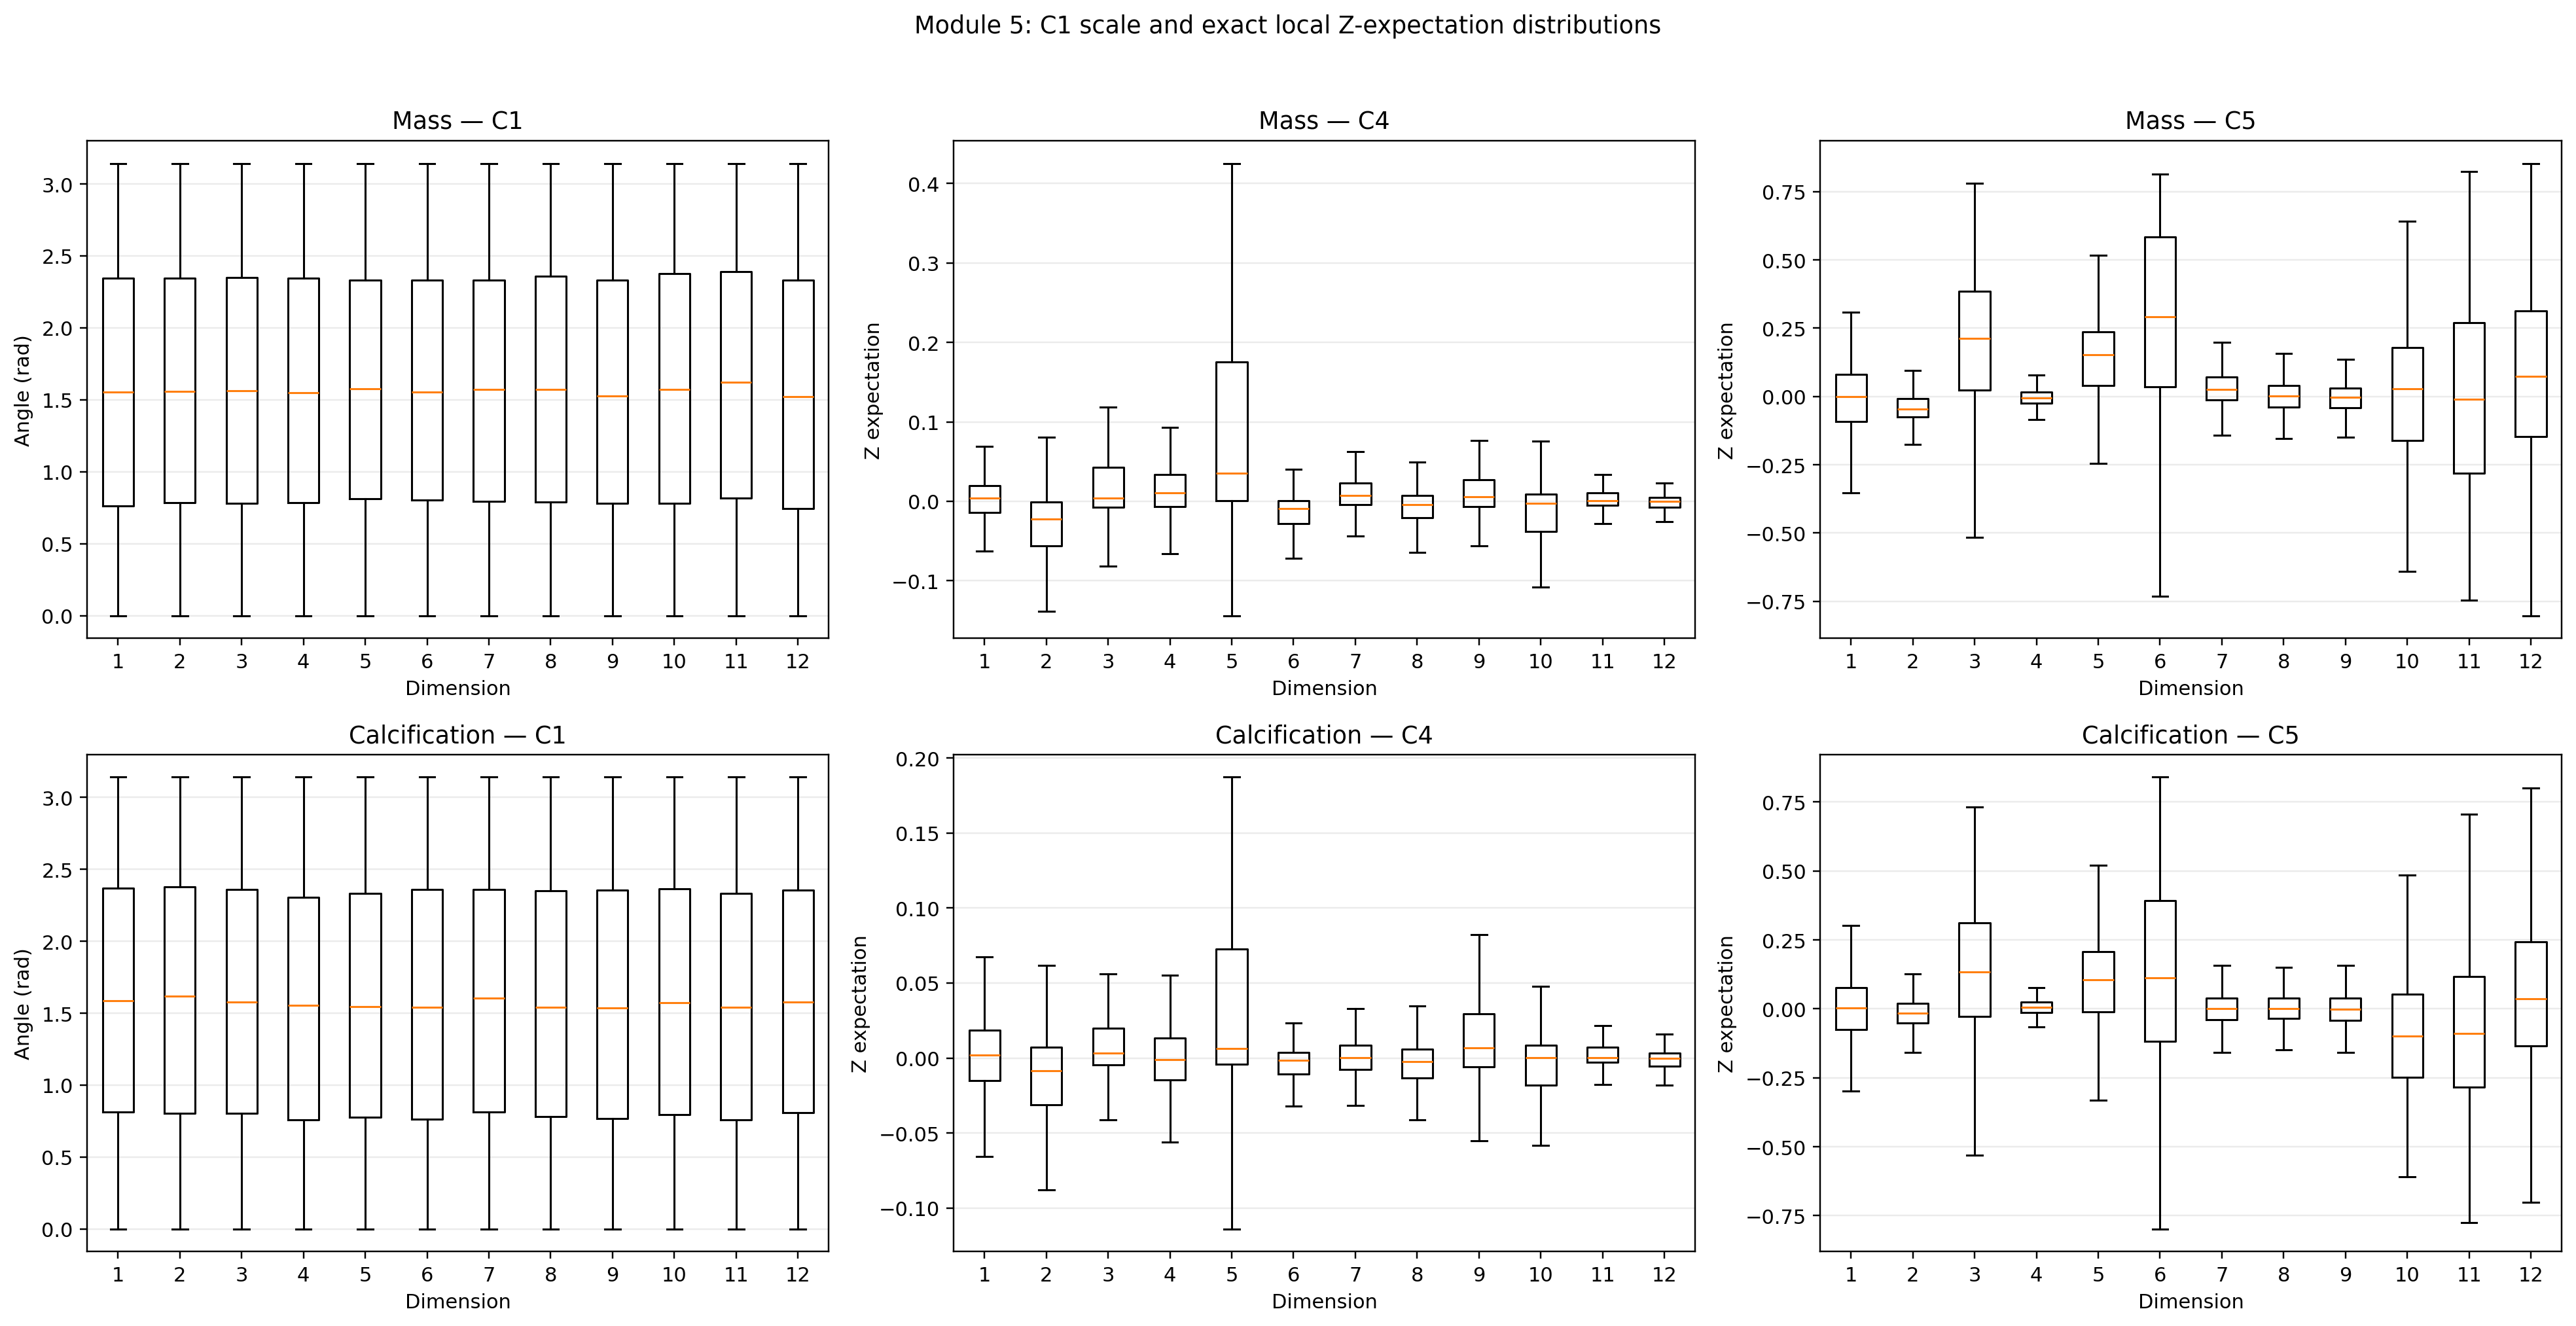
\includegraphics[width=\textwidth]{Figures/M5_embeddings.png}
% fuente: D-014
\caption{Distribución empírica de los valores esperados de Pauli locales $\langle Z_i \rangle$ generados por los mapas cuánticos C4 y C5 para cada dimensión del embedding en masas y calcificaciones (Módulo 5).}
\label{fig:anx_m5_embeddings}
\end{figure}

% ------------------------------------------------------------
\subsection{Complejidad, costes y muestreo de estados cuánticos}

\begin{figure}[H]
\centering
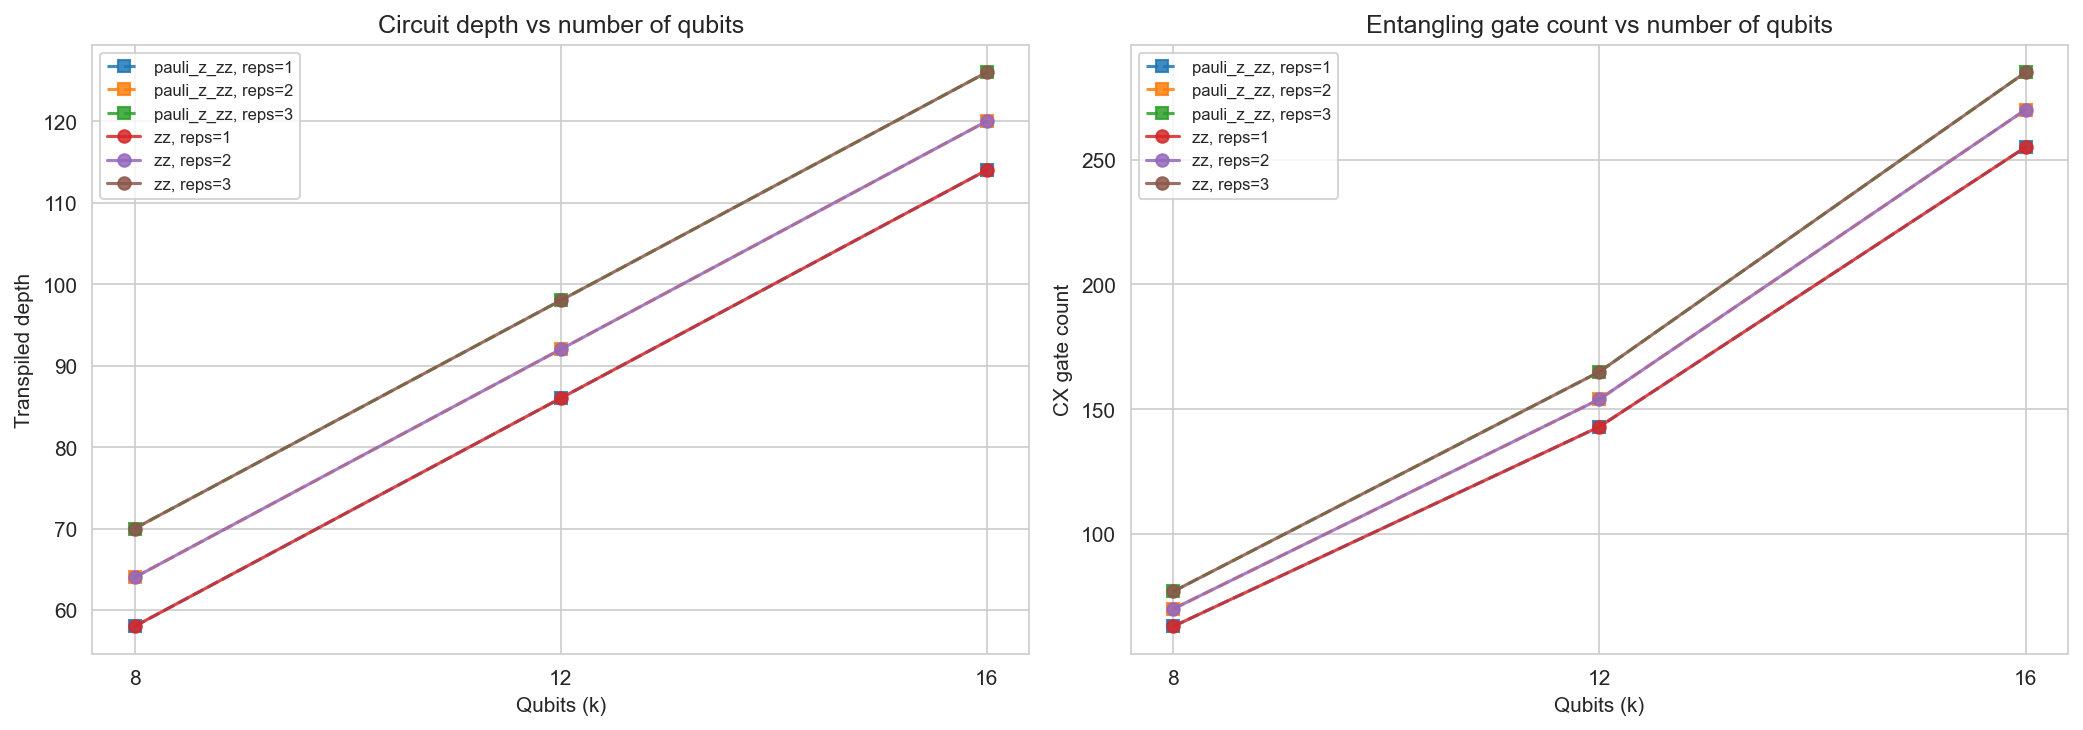
\includegraphics[width=\textwidth]{Figures/E1_circuit_complexity.png}
% fuente: D-013
\caption{Complejidad estructural de los circuitos cuánticos evaluados en función del número de qubits $k$. Se reporta la profundidad total del circuito y el número de compuertas de dos cúbits requeridas para distintas configuraciones.}
\label{fig:anx_e1_complexity}
\end{figure}

\begin{figure}[H]
\centering
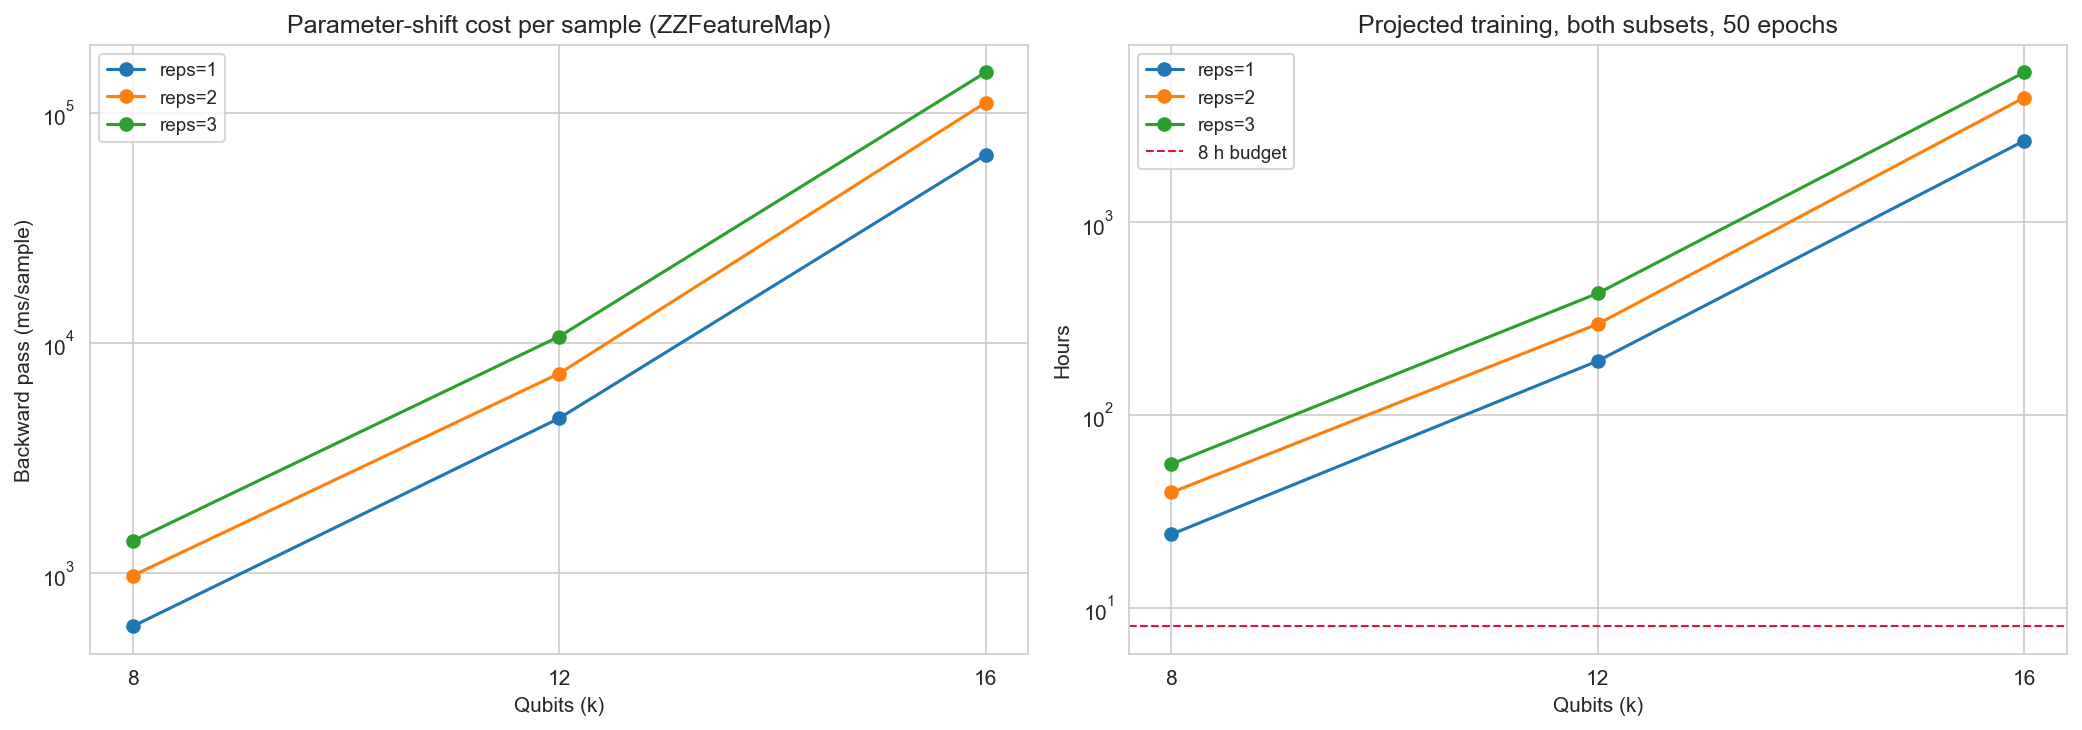
\includegraphics[width=\textwidth]{Figures/E2_training_cost.png}
% fuente: D-013
\caption{Coste computacional del entrenamiento variacional medido en segundos por época y muestra en simuladores cuánticos para diversas topologías de circuito y números de qubits.}
\label{fig:anx_e2_training_cost}
\end{figure}

\begin{figure}[H]
\centering
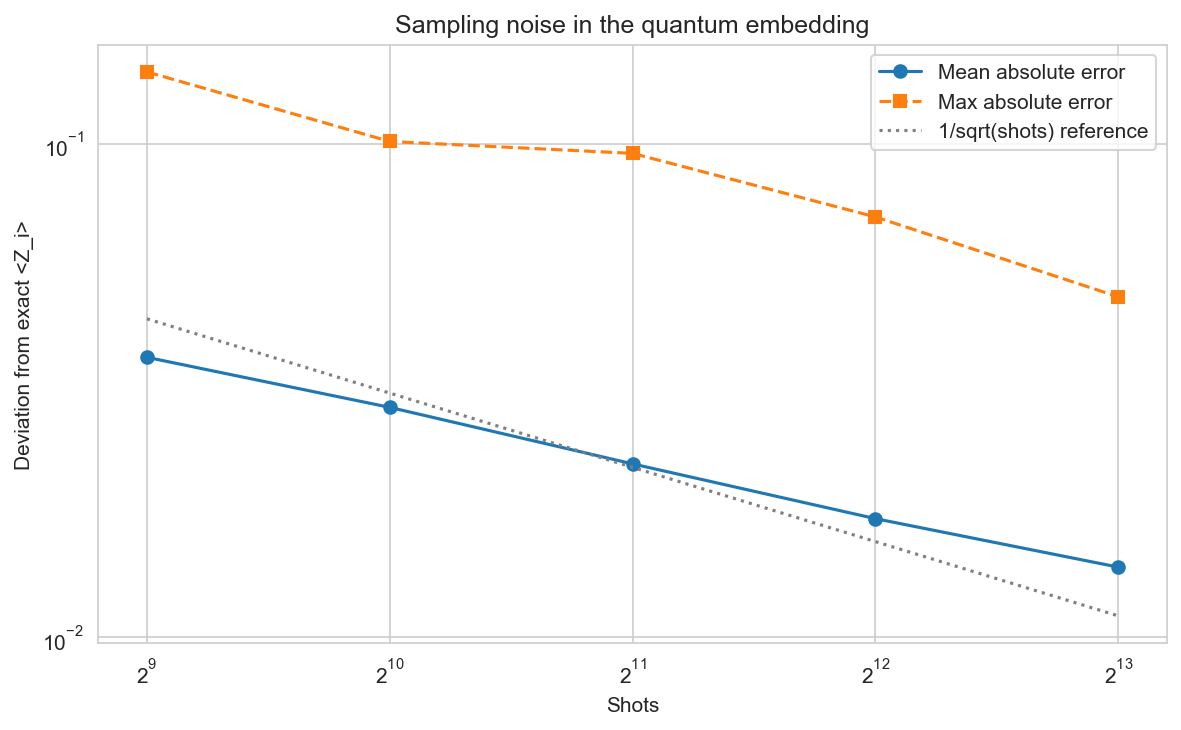
\includegraphics[width=\textwidth]{Figures/E3_shots_sensitivity.png}
% fuente: H-016, H-019
\caption{Sensibilidad del error de estimación al número de disparos finitos (\textit{shots}). El aparente estancamiento en precisión observado en la versión preliminar de este análisis respondió a ruido numérico en la referencia de evaluación, según se documentó y subsanó posteriormente en el cuaderno B3 con cálculos exactos.}
\label{fig:anx_e3_shots}
\end{figure}

\begin{figure}[H]
\centering
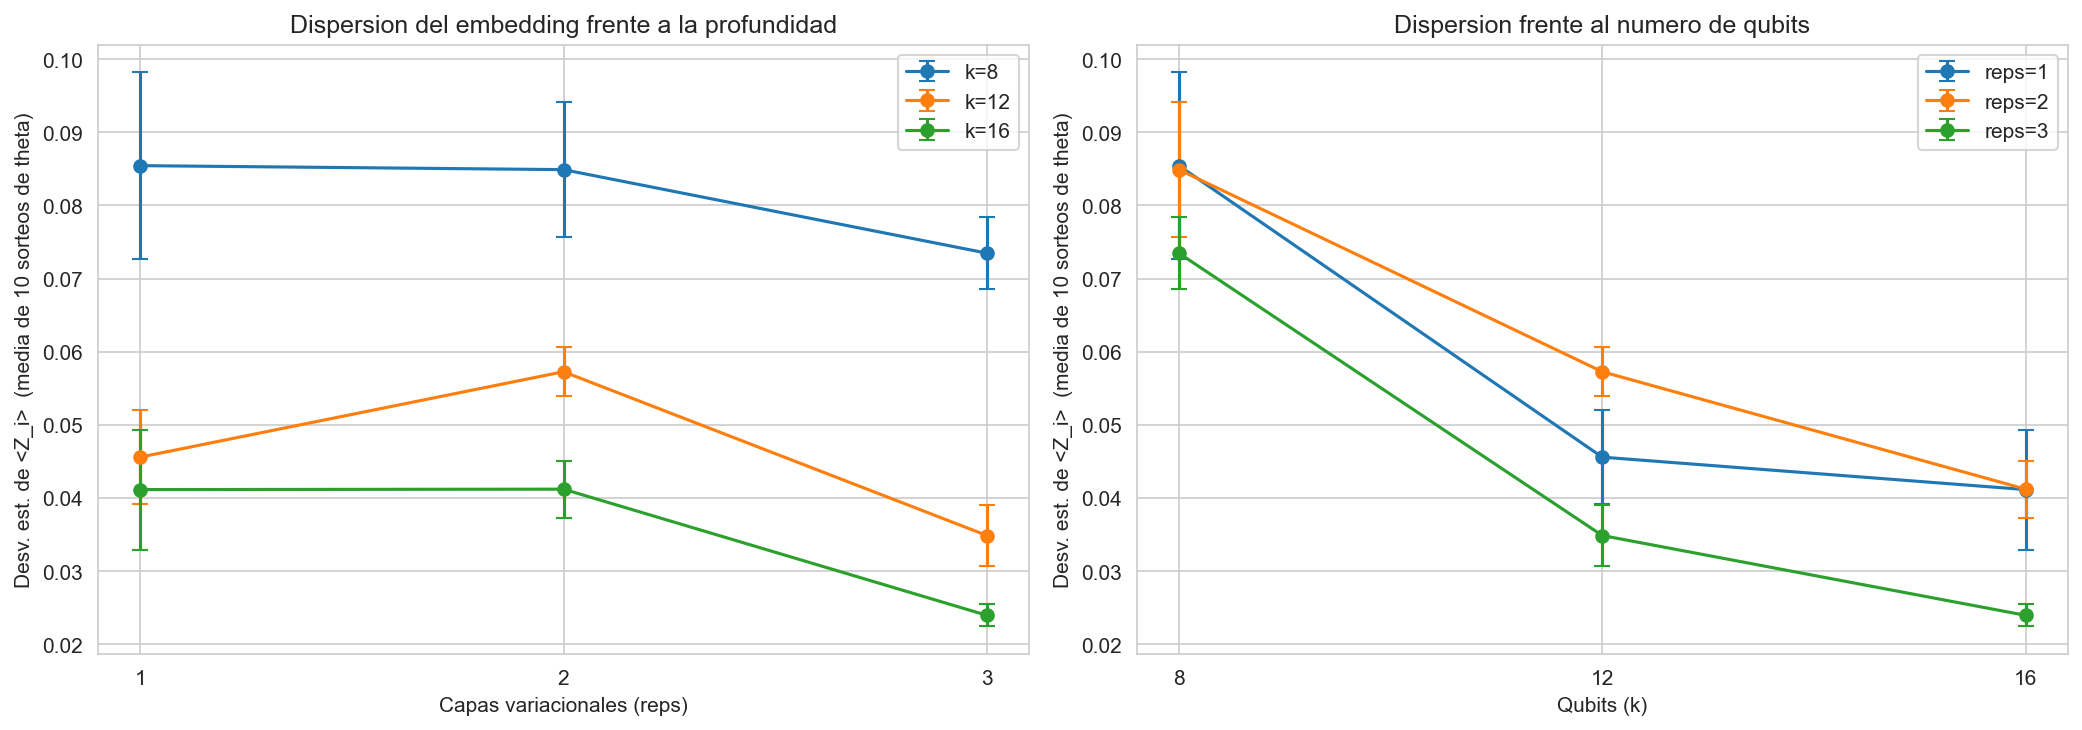
\includegraphics[width=\textwidth]{Figures/E4_embedding_concentration.png}
% fuente: H-018
\caption{Efecto de concentración de medida en el espacio de Hilbert al incrementar el número de qubits $k$. La dispersión entre estados para diferentes lesiones decae exponencialmente conforme aumenta la dimensionalidad cuántica.}
\label{fig:anx_e4_concentration}
\end{figure}

% ------------------------------------------------------------
\subsection{Experimentos complementarios de kernels, dimensionalidad y QSVM}

\begin{figure}[H]
\centering
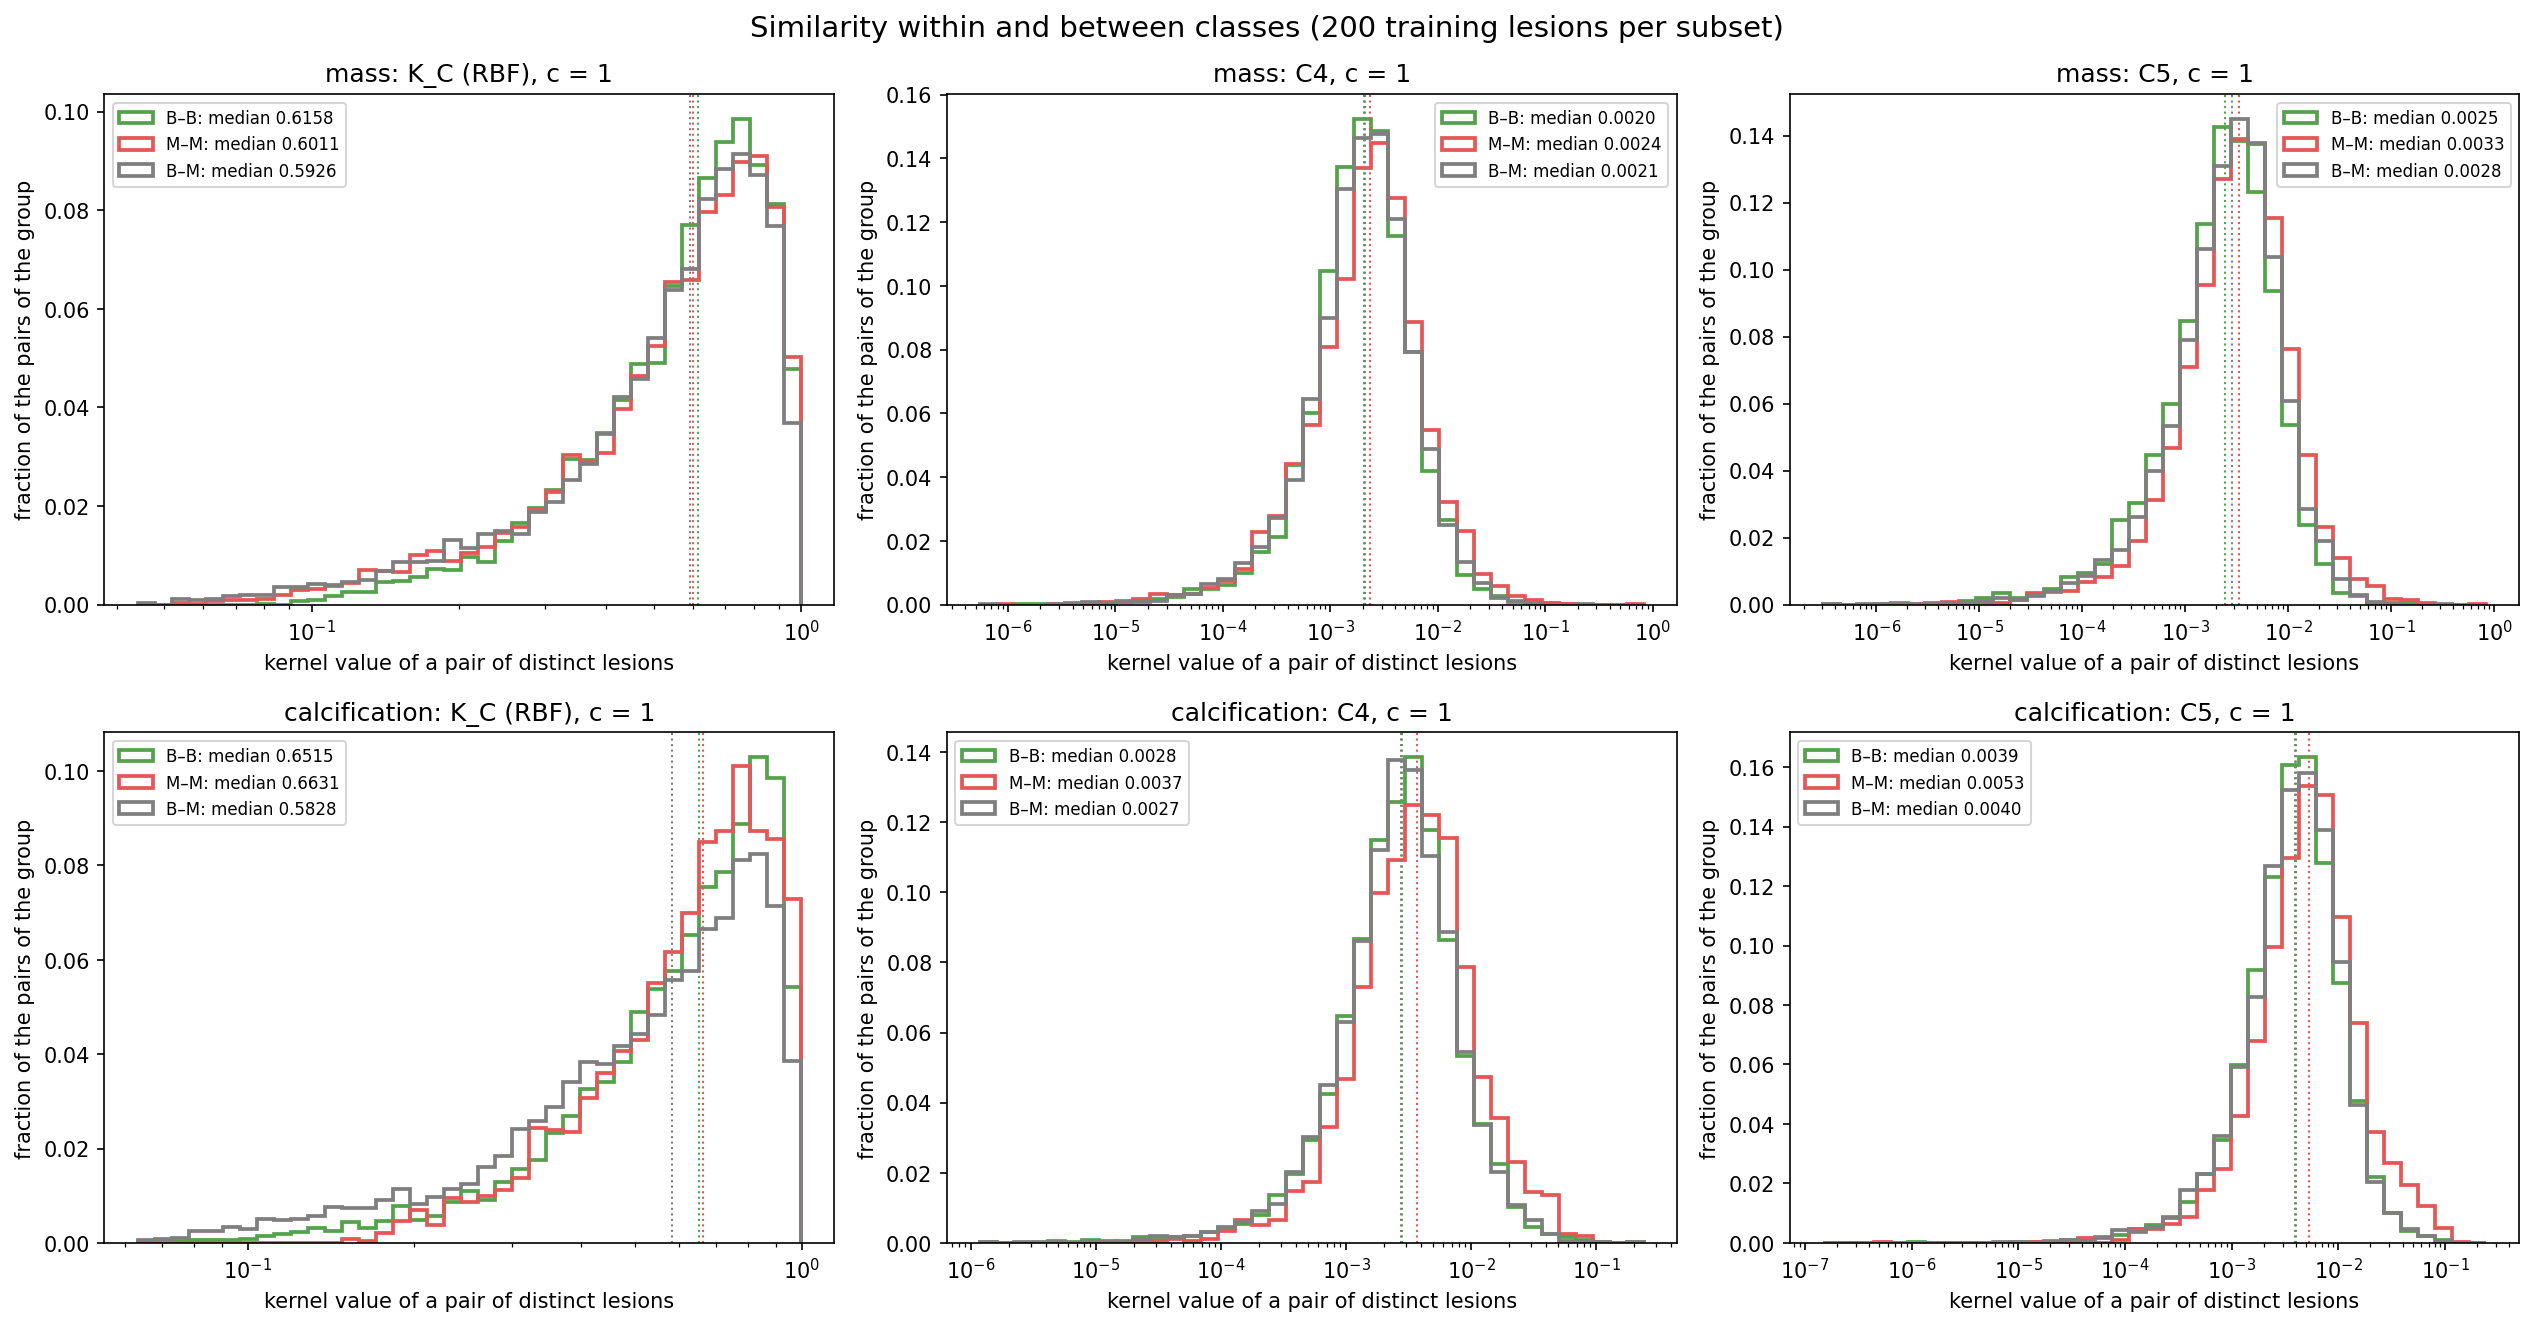
\includegraphics[width=\textwidth]{Figures/X2_kernel_pairs_by_class.png}
% fuente: H-036
\caption{Distribución de valores de similitud en matrices de kernel intraclase e interclase (Experimento X2). Se compara la discriminación obtenida por el kernel clásico RBF frente a los mapas cuánticos C4 y C5 bajo distintos factores de escala angular $c$.}
\label{fig:anx_x2_pairs}
\end{figure}

\begin{figure}[H]
\centering
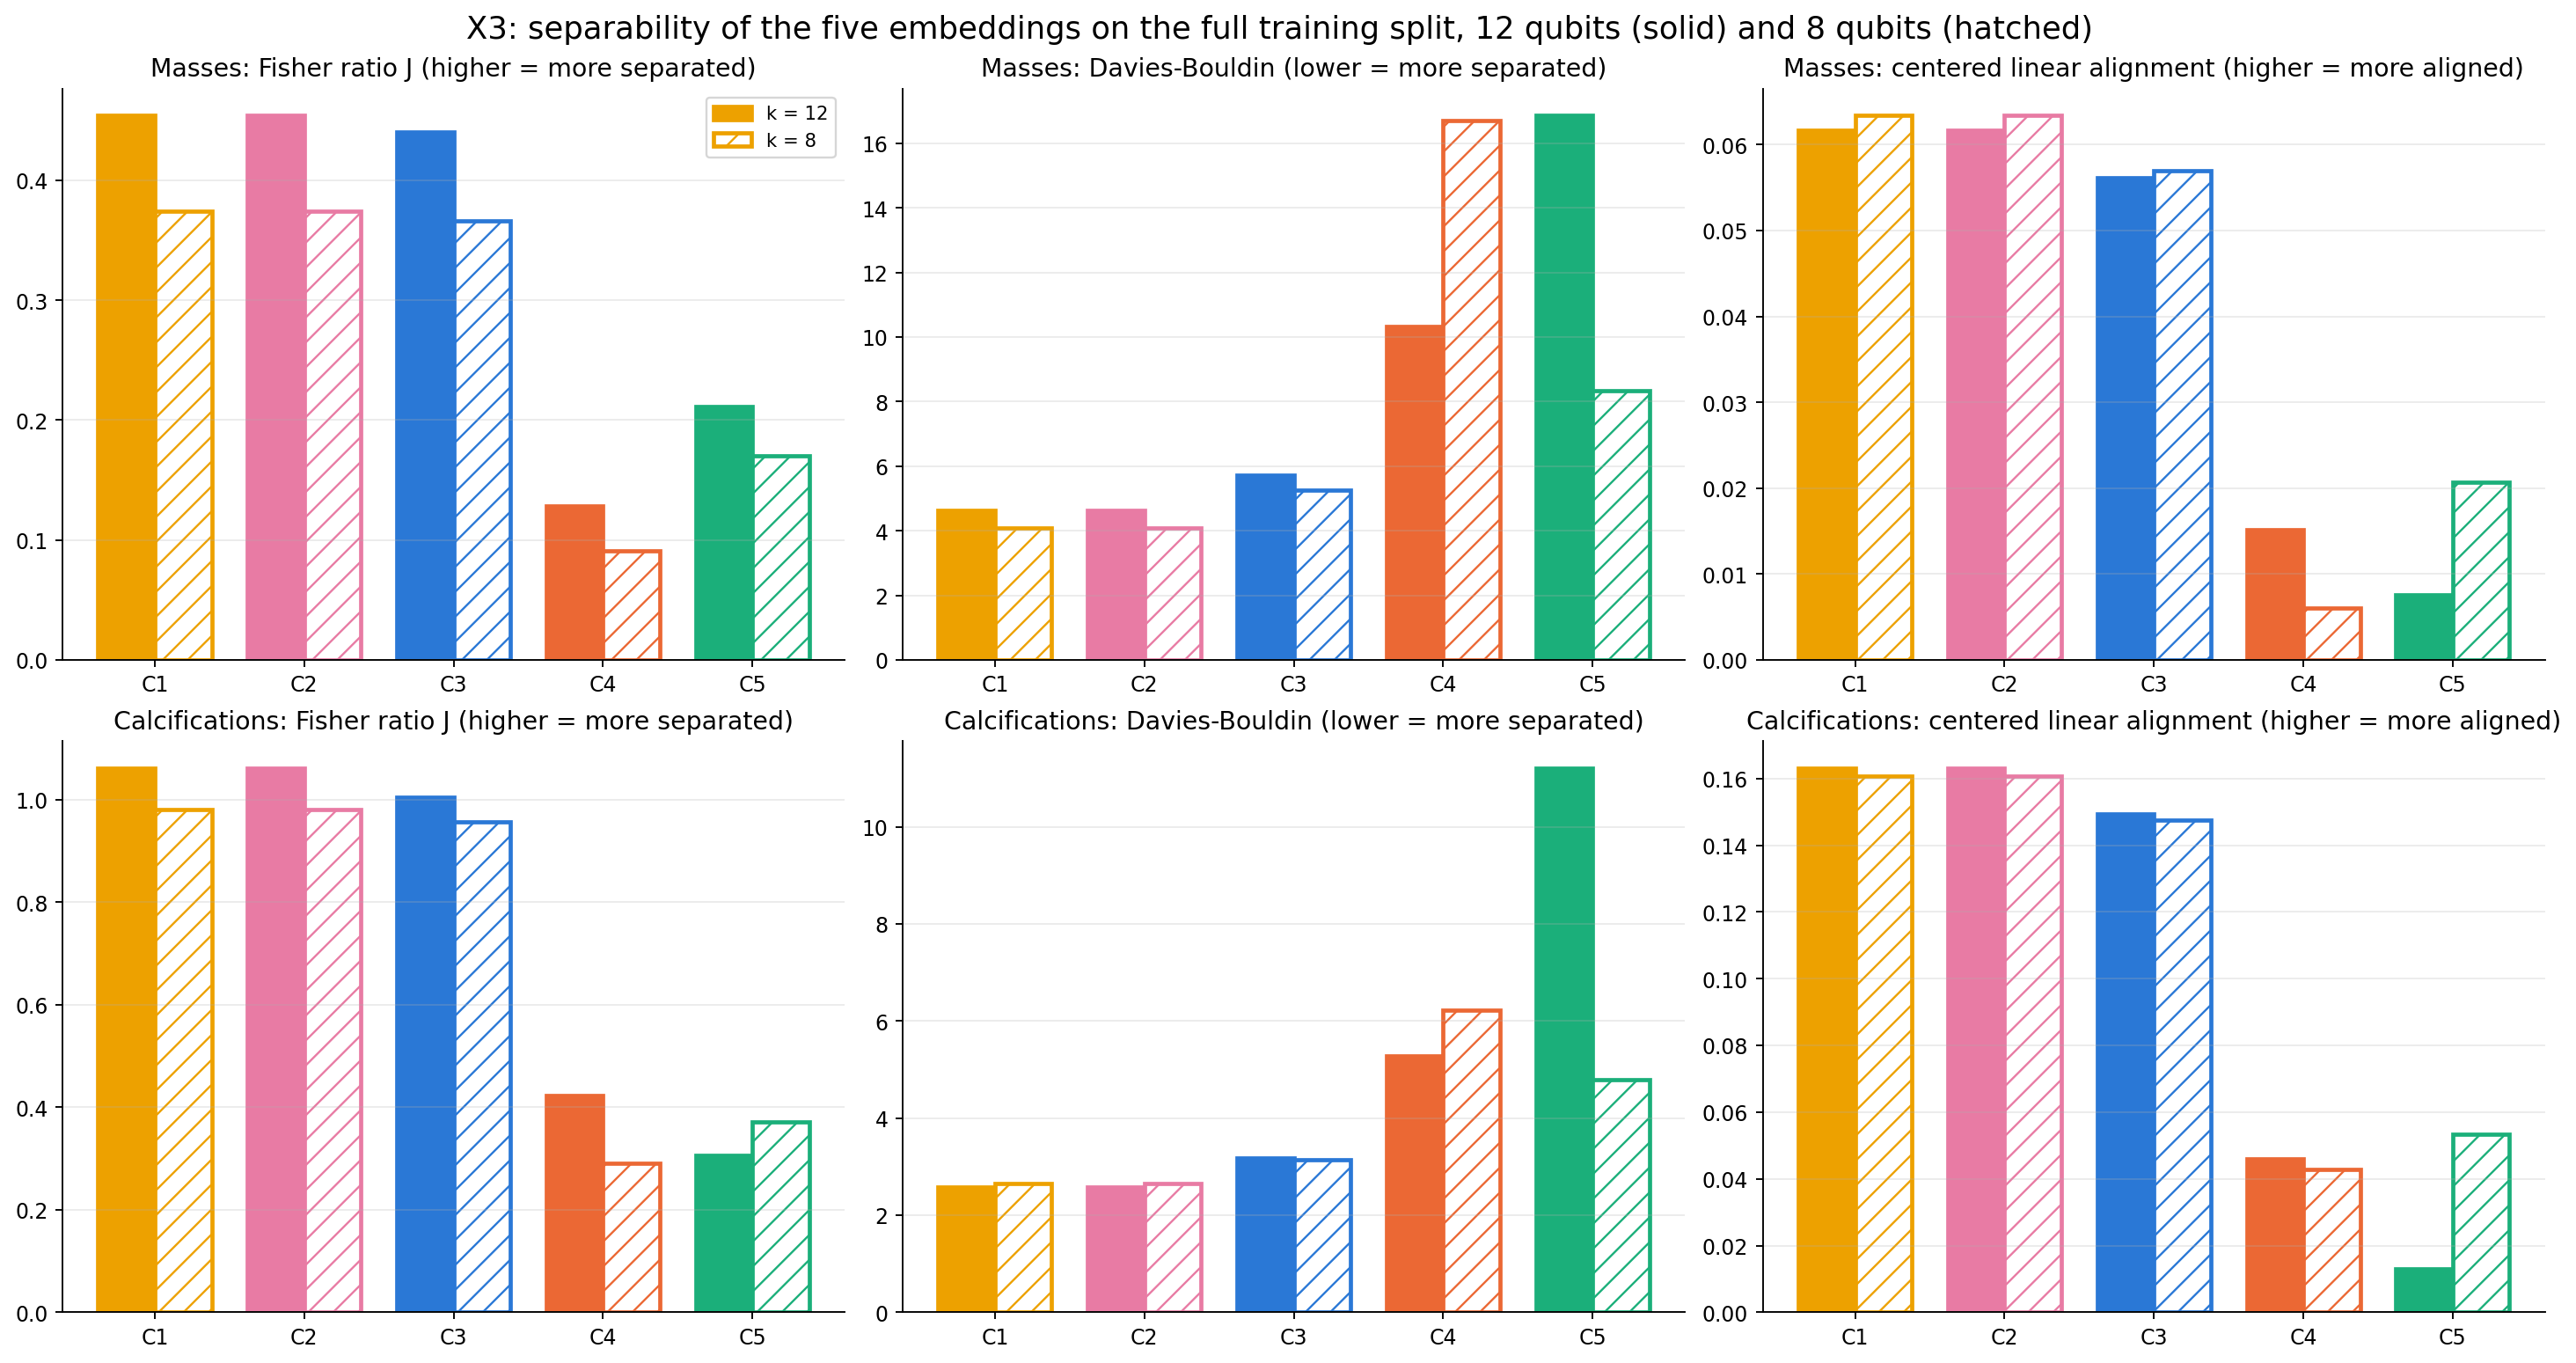
\includegraphics[width=\textwidth]{Figures/X3_embedding_metrics_k8_k12.png}
% fuente: H-041
\caption{Comparativa de métricas de separabilidad geométrica (Davies--Bouldin, Fisher $J$ y alineamiento KTA) entre la configuración reducida de $k = 8$ qubits y el diseño principal de $k = 12$ qubits (Experimento X3).}
\label{fig:anx_x3_k8_k12}
\end{figure}

\begin{figure}[H]
\centering
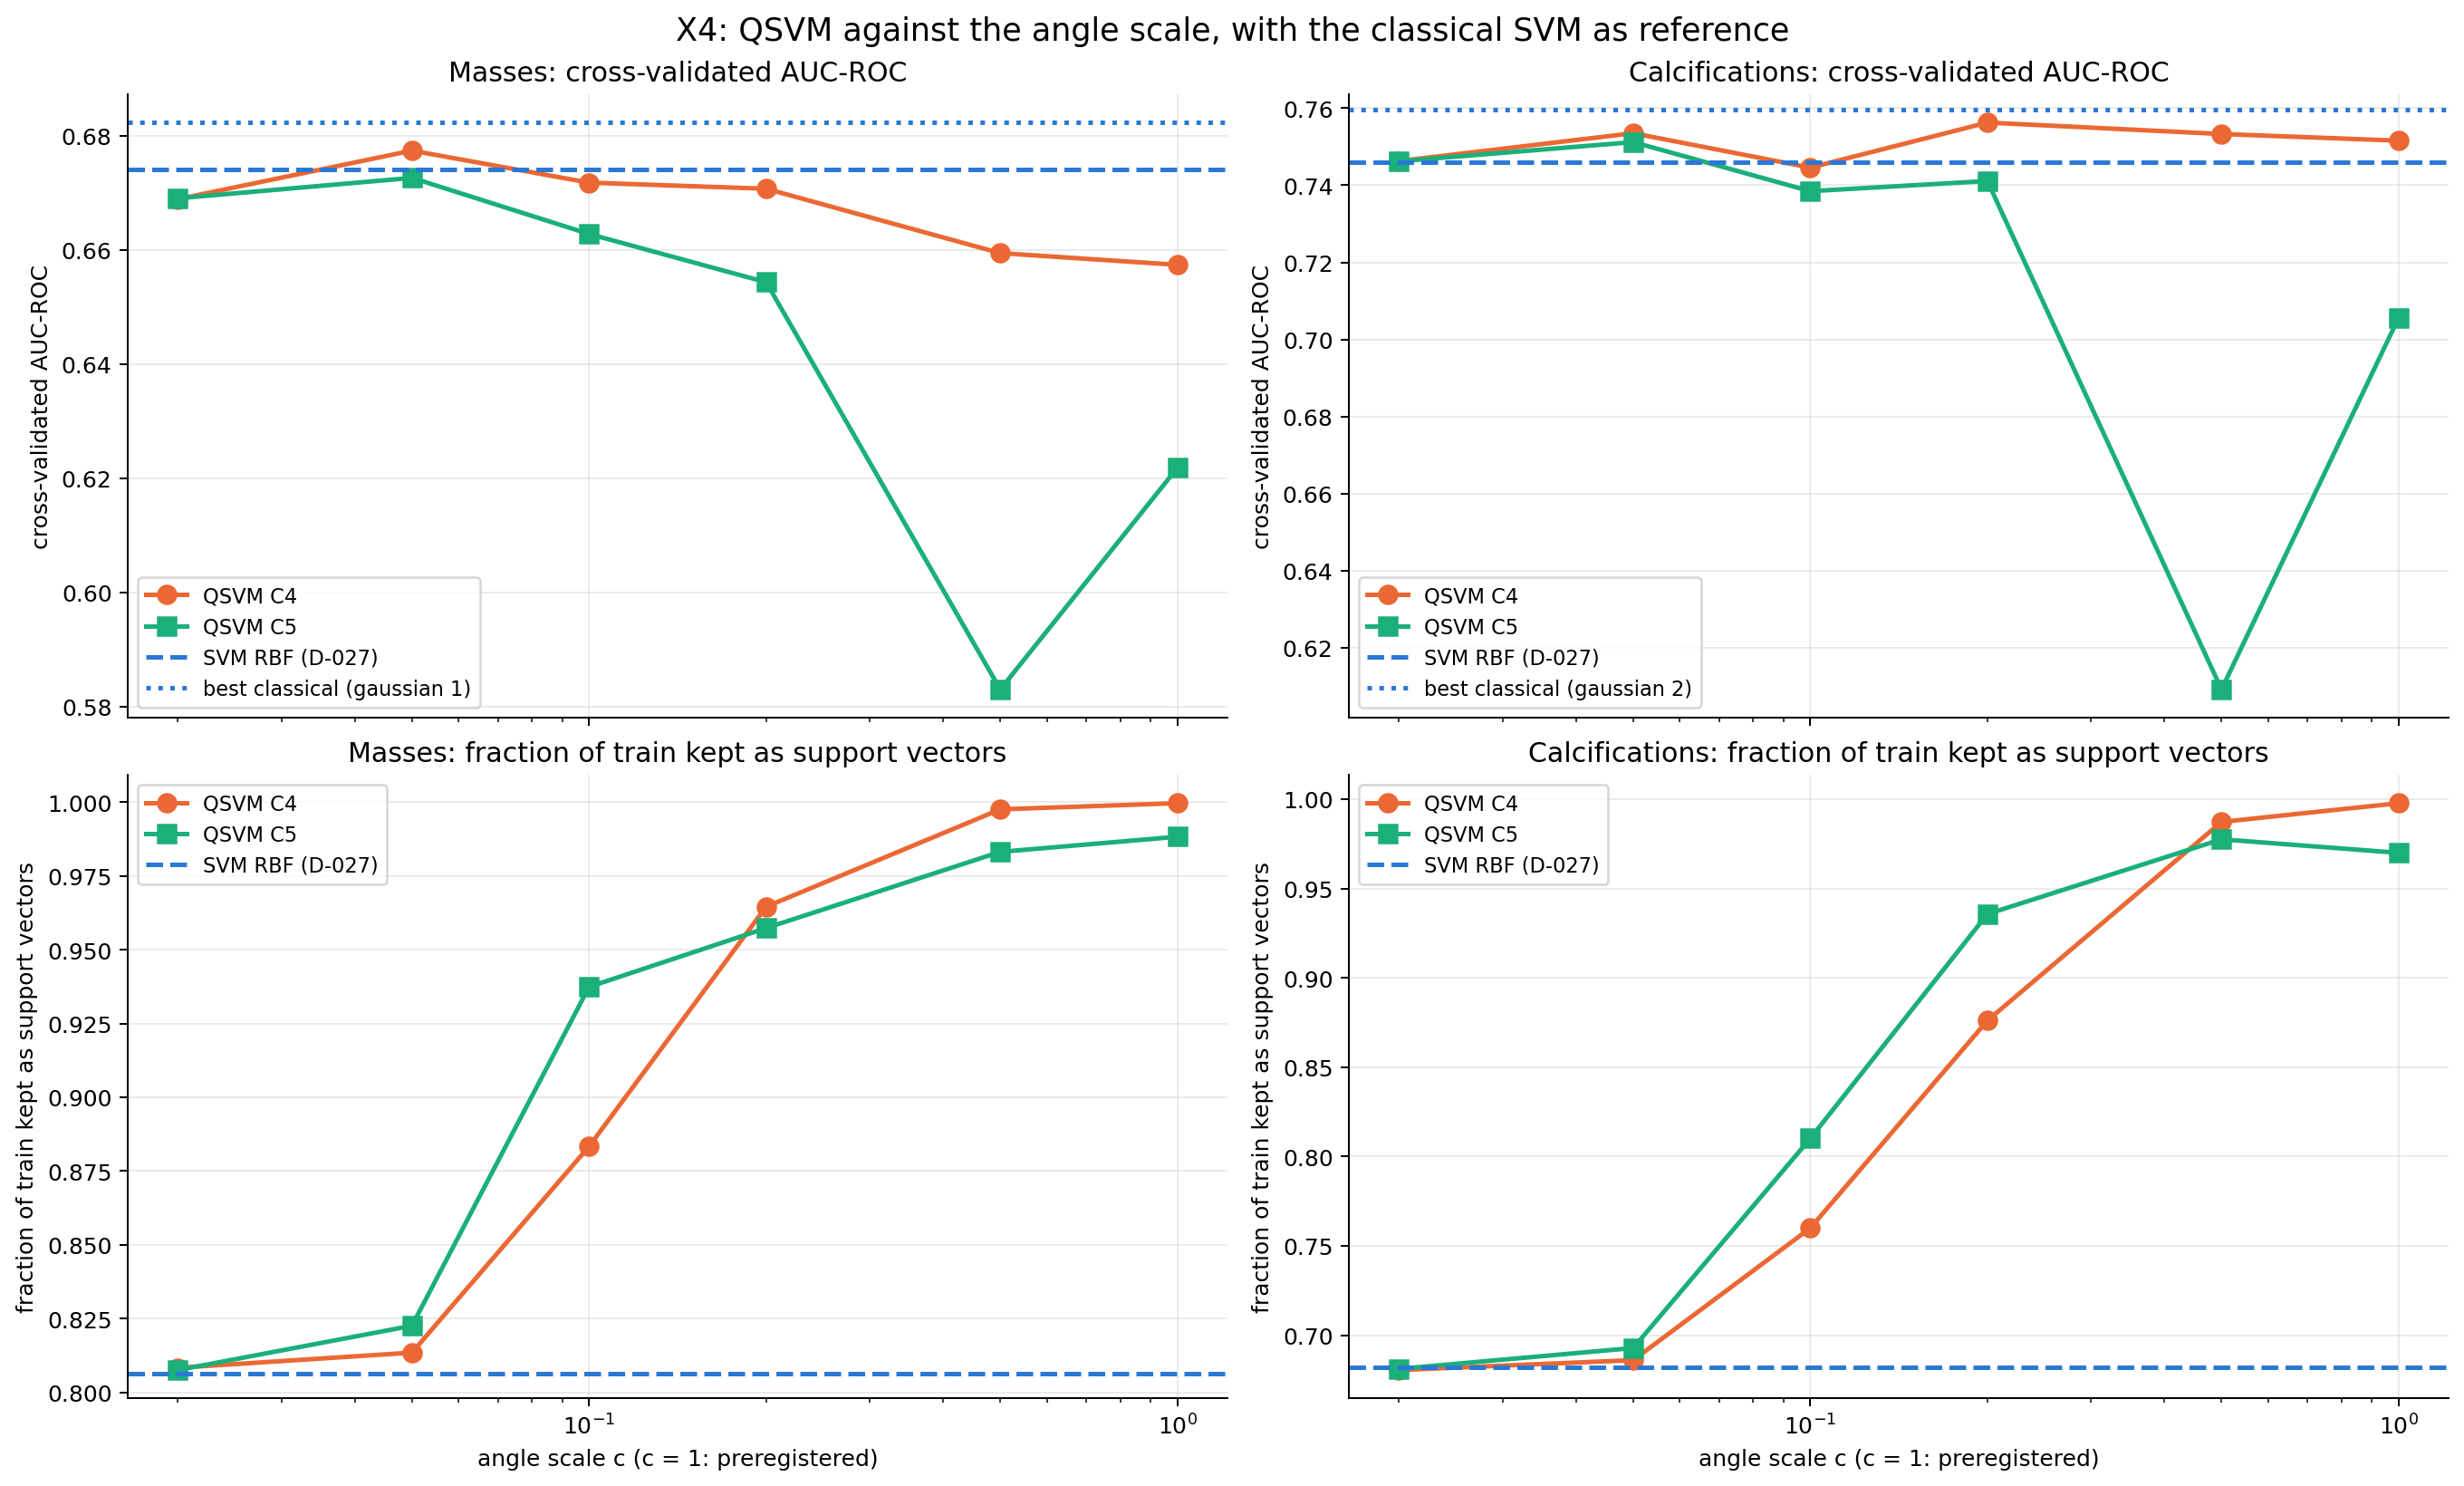
\includegraphics[width=\textwidth]{Figures/X4_qsvm_scale.png}
% fuente: H-044
\caption{Desempeño en clasificación del algoritmo QSVM frente a variaciones en el factor de escala angular $c$ (Experimento X4), contrastado con la referencia clásica de SVM con kernel gaussiano RBF.}
\label{fig:anx_x4_qsvm_scale}
\end{figure}

\begin{figure}[H]
\centering
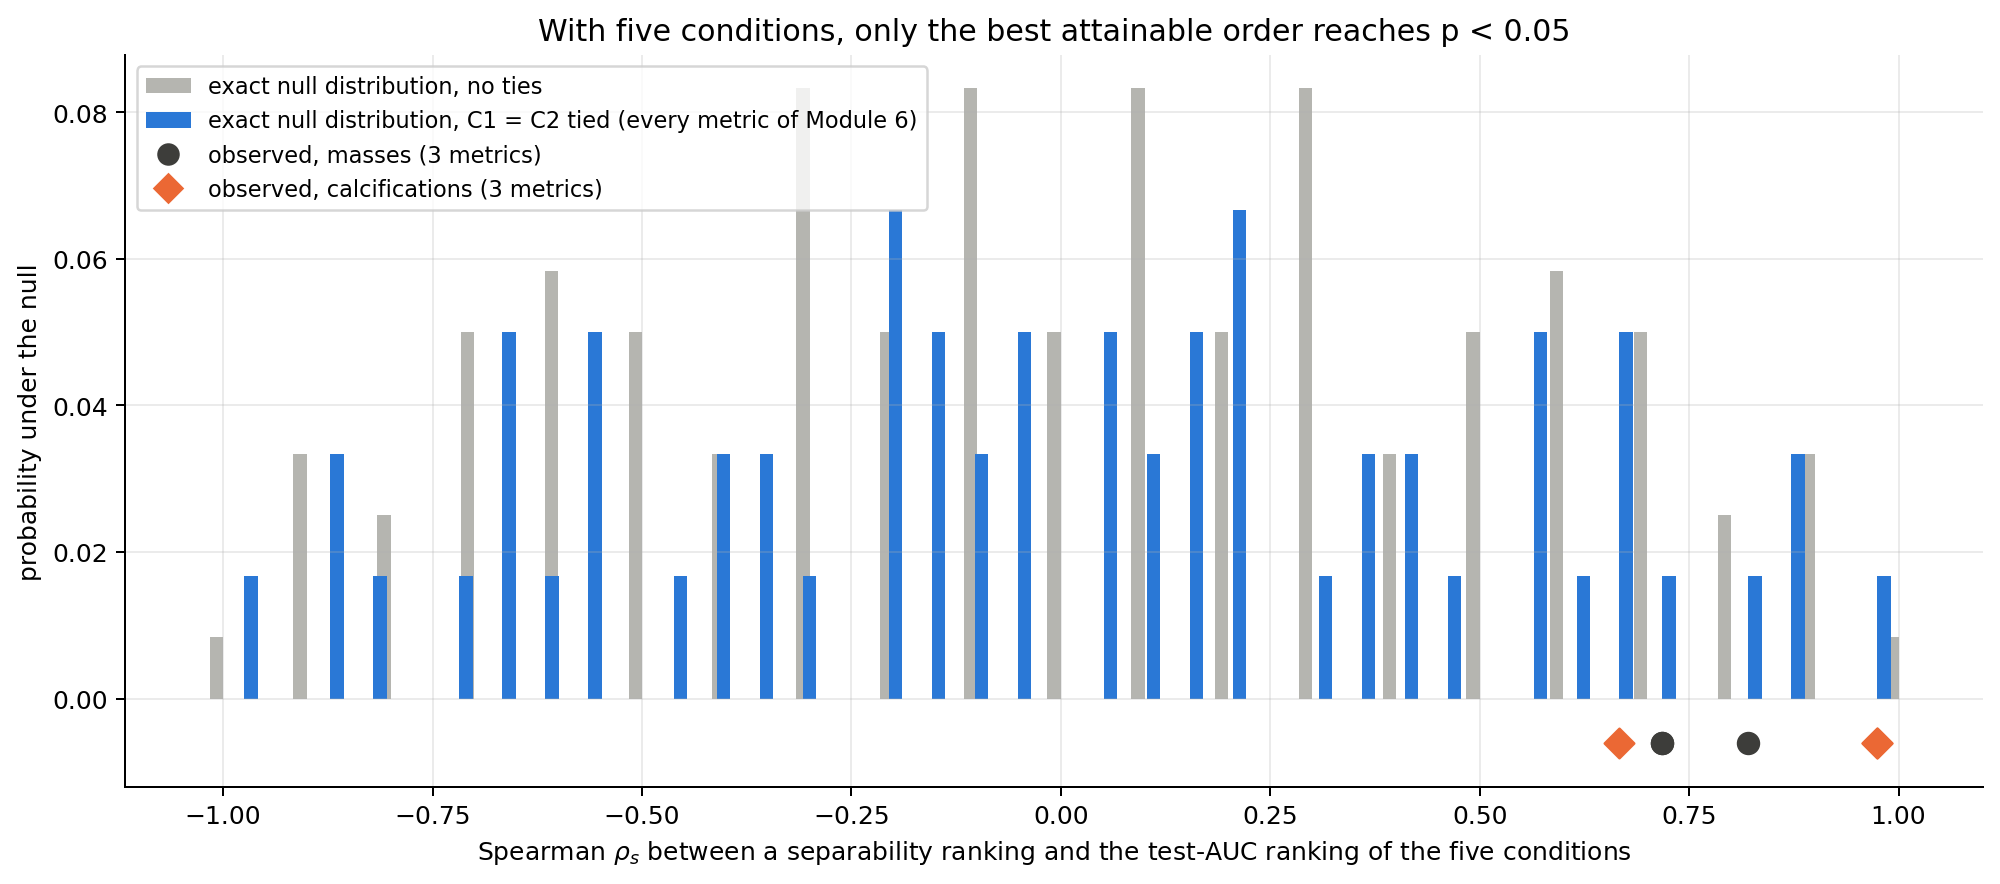
\includegraphics[width=0.85\textwidth]{Figures/M8_spearman_null.png}
% fuente: H-049
\caption{Distribución nula exacta del estadístico de correlación de Spearman $\rho_s$ generada a partir de las 120 permutaciones exhaustivas de las cinco condiciones experimentales con rangos promedio por empates (Módulo 8).}
\label{fig:anx_m8_spearman_null}
\end{figure}

% ---
% Figuras complementarias del Análisis Exploratorio de Datos (Capítulo 4).
% Decisiones y hallazgos que lo respaldan: D-005, D-006, D-009, D-022, H-001, H-002, H-050.
% ---

\subsection{Figuras del análisis exploratorio}
\label{anx:figuras_eda}

Las siguientes figuras complementan la caracterización realizada en el
capítulo~\ref{sec:eda}, reuniendo aquellas distribuciones de clases,
metadatos clínicos, características de escáner e intensidades de píxeles
trasladadas del cuerpo principal para optimizar la concisión del reporte técnico.

\begin{figure}[htbp]
  \centering
  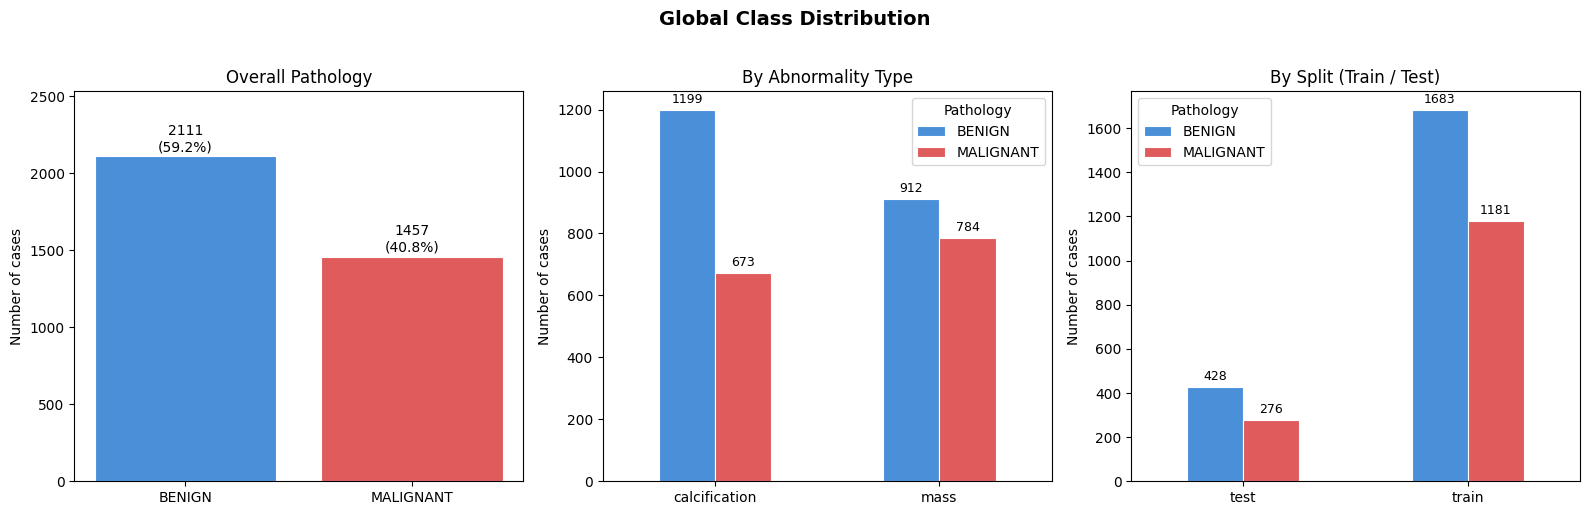
\includegraphics[width=\textwidth]{Figures/B1_class_distribution.png}
  \caption{Distribución de clases global, por tipo de hallazgo y por split train/test.}
  \label{fig:class_distribution}
\end{figure}

\begin{figure}[htbp]
  \centering
  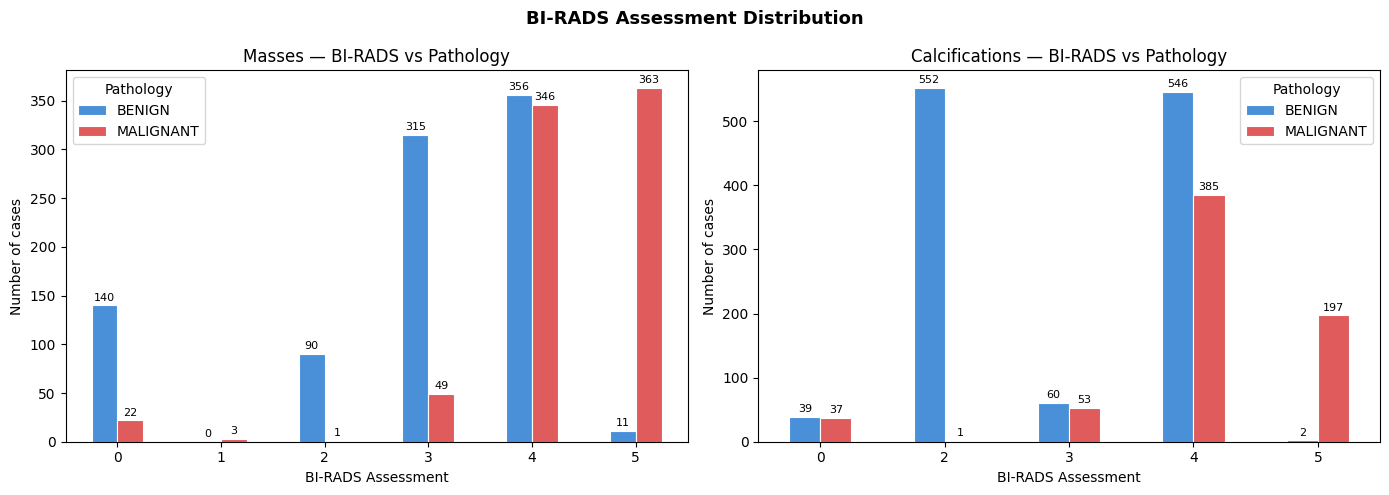
\includegraphics[width=\textwidth]{Figures/B3_birads_distribution.png}
  \caption{Distribución de categorías BI-RADS por patología y tipo de hallazgo.}
  \label{fig:birads_distribution}
\end{figure}

\begin{figure}[htbp]
  \centering
  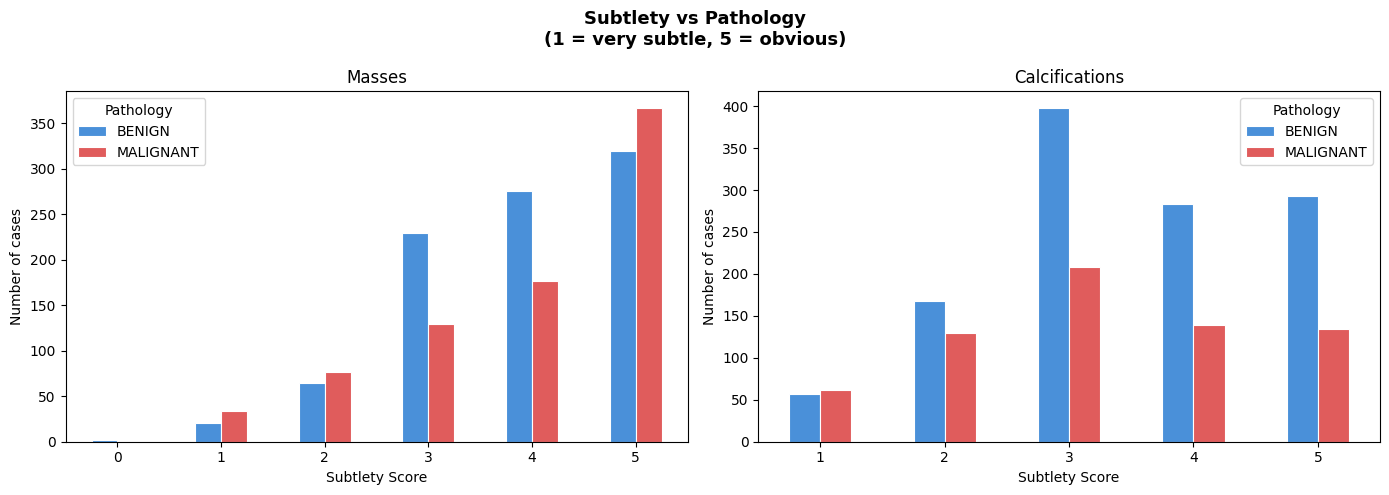
\includegraphics[width=\textwidth]{Figures/B4_subtlety_distribution.png}
  \caption{Distribución de \textit{subtlety} por patología y tipo de hallazgo (1\,=\,muy sutil, 5\,=\,obvio).}
  \label{fig:subtlety_distribution}
\end{figure}

\begin{figure}[htbp]
  \centering
  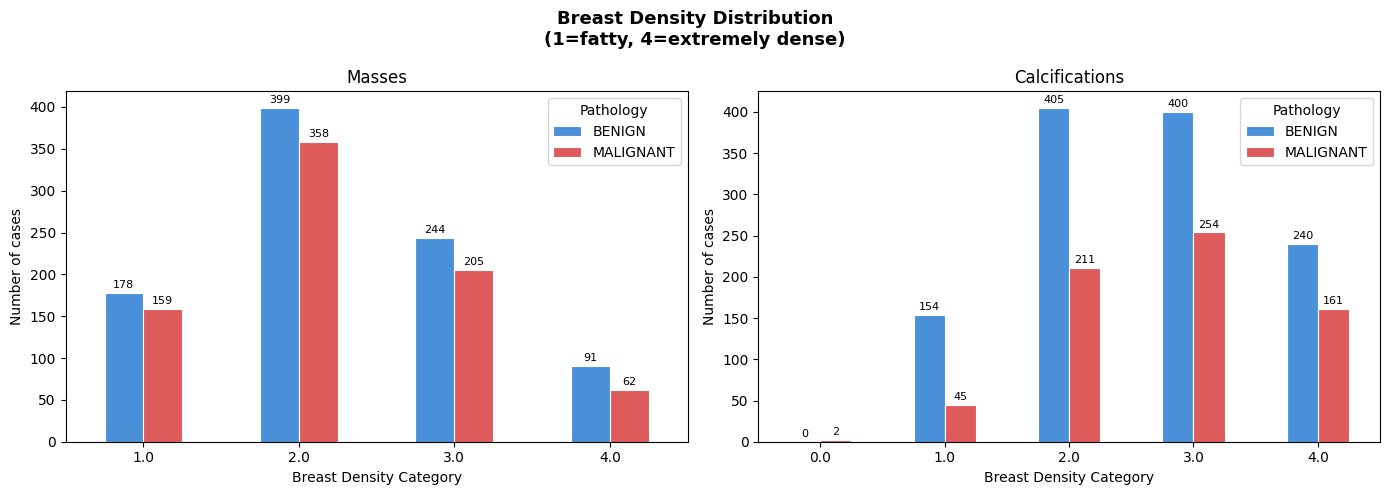
\includegraphics[width=\textwidth]{Figures/C1_breast_density.png}
  \caption{Distribución de densidad mamaria (1\,=\,grasa, 4\,=\,extremadamente densa) por patología y tipo de hallazgo.}
  \label{fig:breast_density}
\end{figure}

\begin{figure}[htbp]
  \centering
  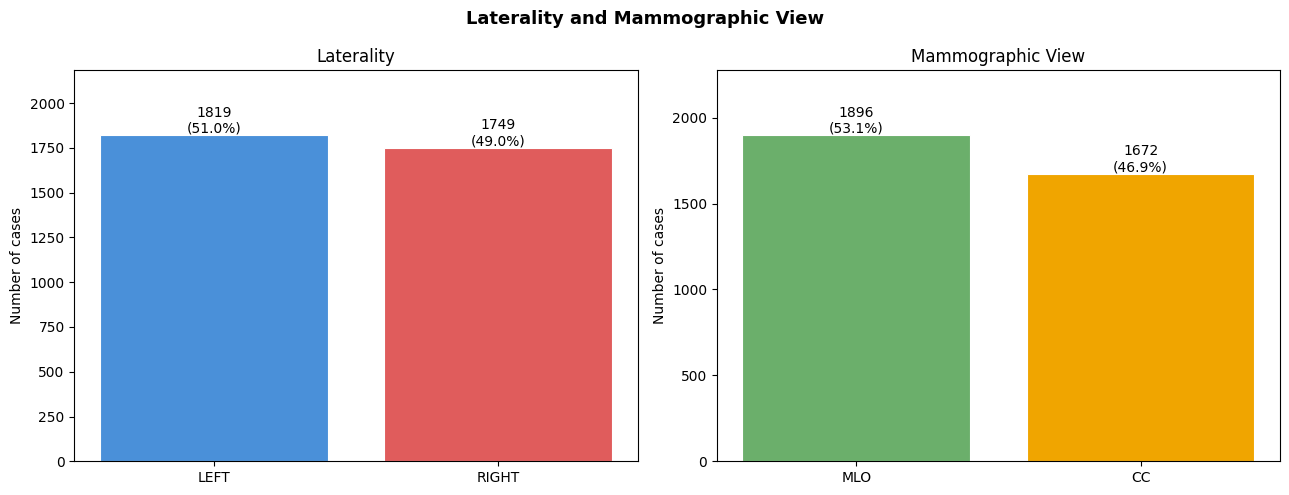
\includegraphics[width=\textwidth]{Figures/C2_laterality_view.png}
  \caption{Distribución de lateralidad y vista mamográfica en el dataset.}
  \label{fig:laterality_view}
\end{figure}

\begin{figure}[htbp]
  \centering
  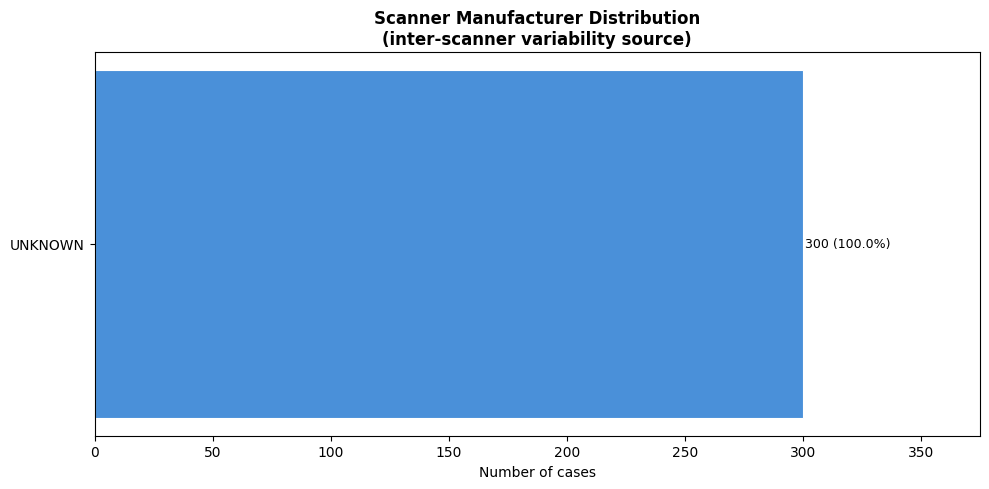
\includegraphics[width=0.8\textwidth]{Figures/D2_manufacturers.png}
  \caption{Distribución de fabricantes de escáner en la muestra analizada.}
  \label{fig:manufacturers}
\end{figure}

\begin{figure}[htbp]
  \centering
  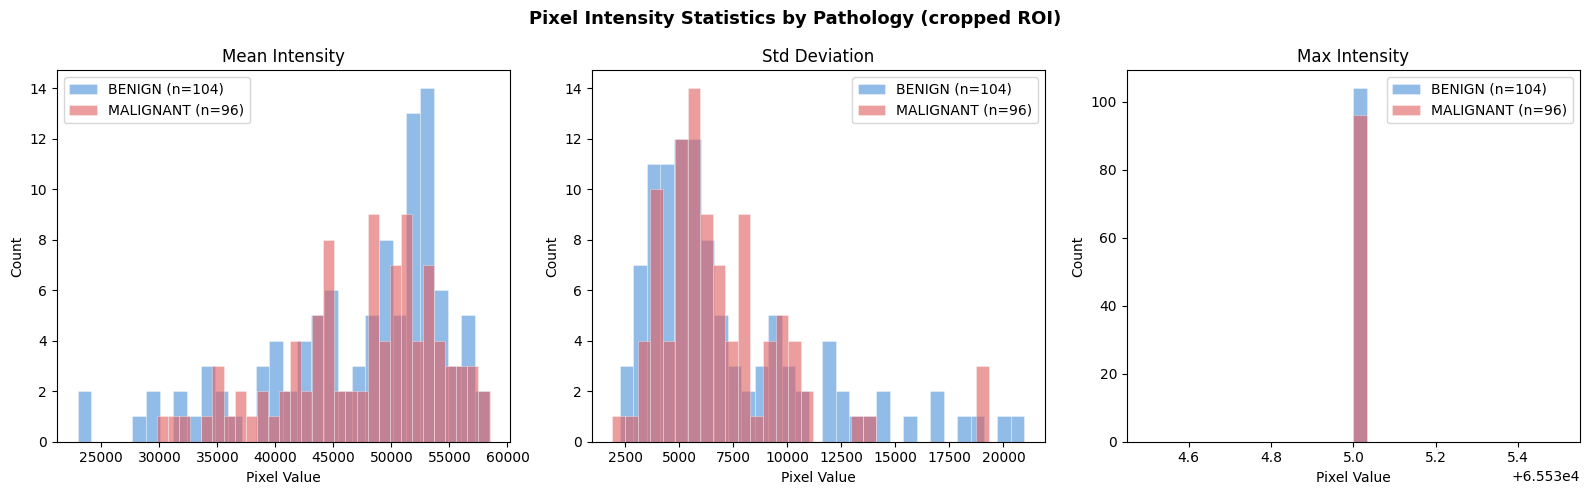
\includegraphics[width=\textwidth]{Figures/D3_pixel_intensities.png}
  \caption{Distribución de estadísticas de intensidad de píxeles (media, desviación estándar y máximo) en imágenes recortadas de ROI, por patología.}
  \label{fig:pixel_intensities}
\end{figure}

\begin{figure}[htbp]
  \centering
  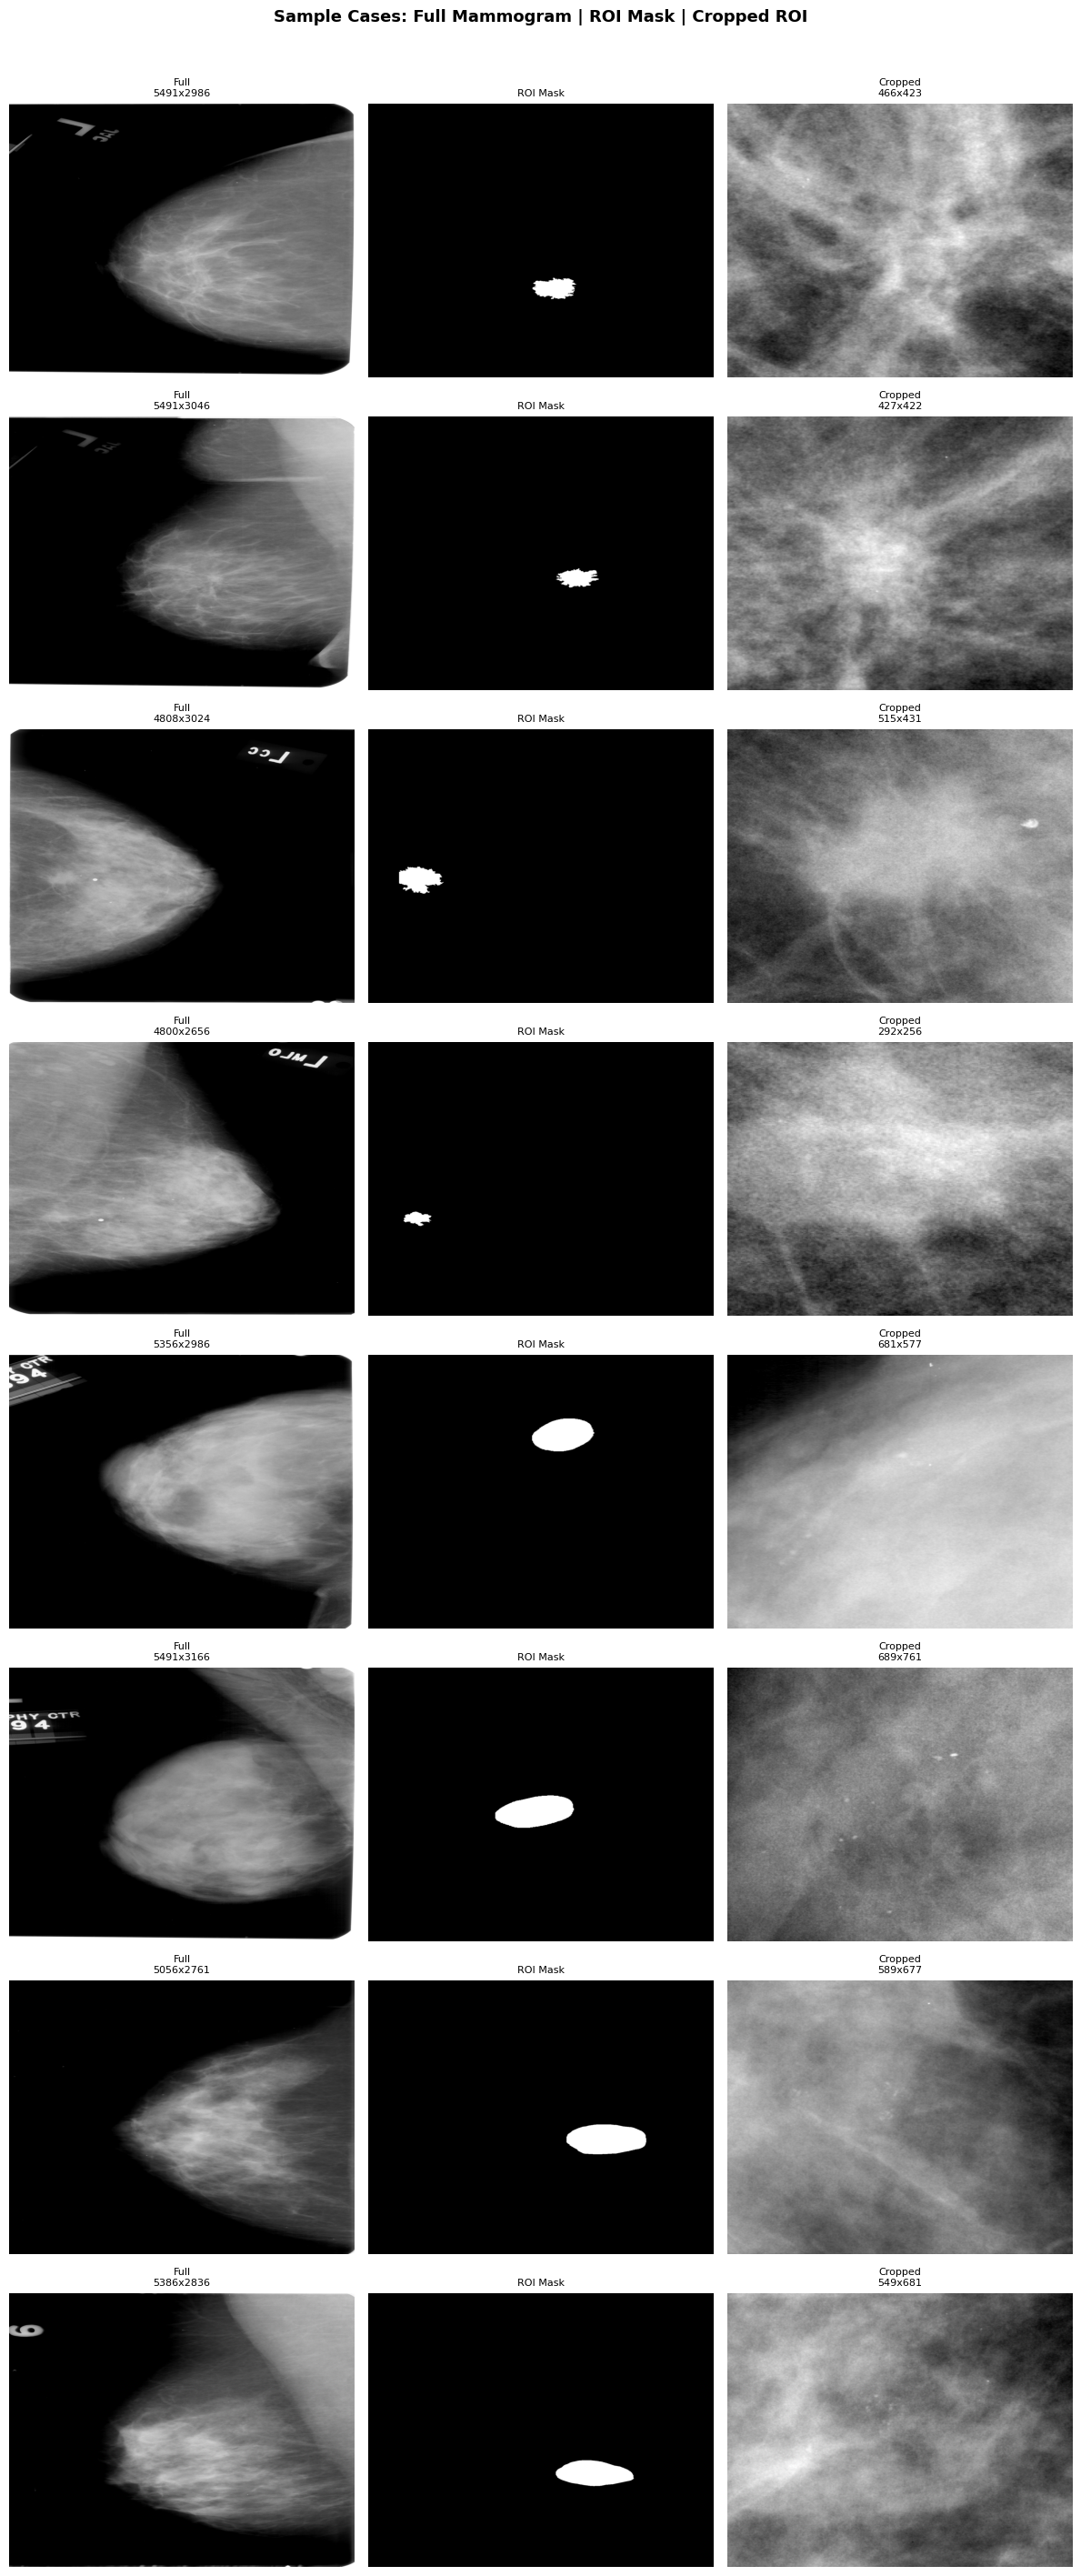
\includegraphics[width=0.7\textwidth, height=0.72\textheight, keepaspectratio]{Figures/D4_sample_gallery.png}
  \caption{Galería de casos representativos: mamografía completa, máscara ROI e imagen recortada, para masas y calcificaciones benignas y malignas.}
  \label{fig:sample_gallery}
\end{figure}

% ============================================================
% ANEXO D · ENTORNO DE EJECUCIÓN Y REPRODUCIBILIDAD
% Especificaciones de software, compilación nativa, hardware y semillas.
% Decisiones que lo respaldan: D-007, D-014, D-026.
% ============================================================

\section{Entorno de ejecución y reproducibilidad}\label{anx:entorno}

La reproducibilidad computacional del pipeline depende del control estricto de las versiones
de software, la compilación determinista de extensiones nativas en C y la fijación de semillas
pseudoaleatorias en todas las etapas del procesamiento.

% ------------------------------------------------------------
\subsection{Paquetes y dependencias del sistema}

El desarrollo se articuló en dos entornos independientes de Conda: el entorno \texttt{radiomics},
destinado al preprocesamiento espacial y la extracción de características morfo-texturales
(Módulos 2 y 3), y el entorno \texttt{qml\_cancer}, orientado a la selección estadística,
transformaciones cuánticas variacionales, separabilidad y modelado supervisado (Módulos 4 a 8).
La Tabla~\ref{tab:anexo_d_paquetes} especifica las versiones instaladas de los paquetes fundamentales.

\input{tablas/anexo_d_paquetes}

% ------------------------------------------------------------
\subsection{Procedimiento de compilación de PyRadiomics}

% fuente: D-007
La librería PyRadiomics no admite instalación directa desde los repositorios de PyPI debido a que
la distribución fuente de la versión 3.1.0 declara inconsistencias de versión en sus metadatos y omite
en su manifiesto los archivos de cabecera \texttt{cmatrices.h} y \texttt{cshape.h}, impidiendo la compilación.
Tampoco existe un paquete de PyRadiomics en conda-forge.

Por ello, la biblioteca se compiló directamente a partir del código fuente del repositorio oficial
de AIM-Harvard fijado en el commit \texttt{8ed579383b44806651c463d5e691f3b2b57522ab}. La compilación
se efectuó empleando \texttt{scikit-build-core} y \texttt{setuptools\_scm}, enlazando las extensiones
nativas en C directamente contra el entorno local sin aislamiento de construcción
(\texttt{-\allowbreak-no-\allowbreak build-\allowbreak isolation}) para prevenir actualizaciones accidentales de NumPy que pudiesen comprometer la interoperabilidad con Qiskit.

% ------------------------------------------------------------
\subsection{Especificaciones de hardware y plataforma}

Todas las mediciones temporales, consumos de memoria y ejecuciones de simulación exacta reportados
fueron llevados a cabo en una estación de trabajo homogénea con las siguientes especificaciones:

\begin{itemize}
  \item \textbf{Procesador:} Apple M3 con microarquitectura ARM64 de 8 núcleos (4 núcleos de rendimiento y 4 de eficiencia energética).
  \item \textbf{Memoria principal:} 16\,GB de memoria unificada LPDDR5 (\texttt{hw.memsize}: 17\,179\,869\,184 bytes).
  \item \textbf{Sistema operativo:} macOS Sonoma versión 26.6.2 (Darwin Kernel versión 25G83).
\end{itemize}

% ------------------------------------------------------------
\subsection{Semillas aleatorias y verificación de reproducción determinista}

% fuente: D-014, D-026
Para asegurar la reproducibilidad bit a bit de todos los experimentos se definieron semillas deterministas:
\begin{itemize}
  \item \textbf{Semilla global 42:} empleada para la inicialización pseudoaleatoria del vector de parámetros
    variacionales $\theta$ del \textit{ansatz} (D-014), el sorteo de submuestras estratificadas de 200 lesiones
    para análisis geométrico y el generador de números aleatorios en pruebas de permutación.
  \item \textbf{Semillas de pliegues:} semilla 125 para el subconjunto de masas y semilla 168 para el de
    calcificaciones (D-026), seleccionadas tras una búsqueda exhaustiva entre candidatos para minimizar
    la discrepancia máxima en la prevalencia de malignidad entre pliegues.
\end{itemize}

% fuente: CLAUDE.md, «Re-ejecución completa y revisión (8 al 10 oct)»; H-053, H-054, H-055.
% Corregido el 2026-10-19 (auditoría A2-7): el texto anterior no mencionaba X7 a X9 ni las dos excepciones.
Los Módulos 2 al 8, los experimentos complementarios X1 al X6 y los estudios del simulador B2 y B3 se
re-ejecutaron completos entre el 8 y el 10 de octubre de 2026 sobre un clon limpio del repositorio. Las
predicciones, métricas y tablas se reprodujeron bit a bit, con dos excepciones: los tiempos de ejecución y el
muestreo de B3, que no fija semilla. Los experimentos X7, X8 y X9 se ejecutaron después (10, 11 y 18 de
octubre) con el mismo entorno y las mismas semillas.

% ============================================================
% ANEXO E · ÍNDICE DE DECISIONES METODOLÓGICAS
% Tabla consolidada de decisiones del proyecto (D-001 a D-040).
% ============================================================

\section{Índice de decisiones metodológicas}\label{anx:decisiones}

La bitácora metodológica completa acompaña al presente reporte técnico como material complementario,
documentando el contexto, los antecedentes, las alternativas analizadas y las justificaciones numéricas
de cada determinación adoptada durante el desarrollo del proyecto. La Tabla~\ref{tab:anexo_decisiones}
recopila el índice cronológico de las 40 decisiones metodológicas registradas (D-001 a D-040), identificando
su estado de vigencia y las secciones correspondientes del cuerpo del reporte que fundamentan.

\input{tablas/anexo_e_decisiones}

\newpage

% ===== Bibliografía completa
\begin{thebibliography}{99}
% --- Referencia 1: OMS ---
  \bibitem{WHO2025}
    World Health Organization. (2025, August 14). \textit{World Health Organization}.
    Retrieved from WHO Web site:
    \url{https://www.who.int/news-room/fact-sheets/detail/breast-cancer}

  % --- Referencia 2: GLOBOCAN Data --- 
  \bibitem{GLOBOCAN2022}
    Freihat, O., Sipos, D., \& Kovacs, A. (2025). Global burden and projections of
    breast cancer incidence and mortality to 2050: a comprehensive analysis of
    GLOBOCAN data. \textit{Frontiers in Public Health}, 13, 1622954.
    \url{https://doi.org/10.3389/fpubh.2025.1622954}

  % --- Referencia 3: BCRF Statistics ---
  \bibitem{BCRF2025}
    Breast Cancer Research Foundation. (2025). Breast cancer statistics and resources.
    Retrieved from \url{https://www.bcrf.org/breast-cancer-statistics-and-resources/}

  % --- Referencia 4: Stop Breast Cancer ---
  \bibitem{StopBreastCancer2025}
    Stop Breast Cancer. (2025). Facts \& figures. Retrieved from
    \url{https://www.stopbreastcancer.org/information-center/facts-figures/}

  % --- Referencia 5: Global Cancer Statistics ---
  \bibitem{GlobalCancerStatistics2024}
    American Cancer Society. (2024). Global cancer statistics. Retrieved from
    \url{https://pressroom.cancer.org/GlobalCancerStatistics2024}

  % --- Referencia 6: Cáncer de Mama en México ---
  \bibitem{CancerMexico2025}
    Consultores Salud. (2025). Cáncer de mama en México. Retrieved from
    \url{https://consultorsalud.com.mx/cancer-de-mama-en-mexico/}

  % --- Referencia 7: INEGI Cáncer de Mama ---
  \bibitem{INEGI2025}
    Instituto Nacional de Estadística y Geografía. (2025). Estadísticas de cáncer de mama.
    Retrieved from \url{https://www.inegi.org.mx/contenidos/saladeprensa/aproposito/2025/EAP_CancerMama_25.pdf}

  % --- Referencia 8: National Breast Cancer Foundation - Early Detection ---
  \bibitem{NBCF2026_EarlyDetection}
    National Breast Cancer Foundation. (2026). Early detection of breast cancer.
    Retrieved from \url{https://www.nationalbreastcancer.org/early-detection-of-breast-cancer/}

  % --- Referencia 9: National Breast Cancer Foundation - Breast Cancer Facts ---
  \bibitem{NBCF2026_Facts}
    National Breast Cancer Foundation. (2026). Breast cancer facts \& statistics.
    Retrieved from \url{https://www.nationalbreastcancer.org/breast-cancer-facts/}

  % --- Referencia 10: Windsong Radiology - Early Detection and Survival Rates ---
  \bibitem{Windsong2026_EarlyDetection}
    Windsong Radiology. (2026). How early detection affects breast cancer survival rates.
    Retrieved from \url{https://windsongwny.com/breast-health/how-early-detection-affects-breast-cancer-survival-rates/}

  % --- Referencia 11: INEGI - Estadísticas de Cáncer de Mama 2023 ---
  \bibitem{INEGI2023}
    Instituto Nacional de Estadística y Geografía. (2023). Estadísticas de cáncer de mama.
    Retrieved from \url{https://www.inegi.org.mx/contenidos/saladeprensa/aproposito/2023/EAP_CMAMA23.pdf}

  % --- Referencia 12: American Cancer Society - Global Cancer Statistics 2024 ---
  \bibitem{GlobalCancerStatistics2024_2}
    American Cancer Society. (2024, April). Global cancer statistics 2024. Retrieved from
    \url{https://pressroom.cancer.org/GlobalCancerStatistics2024}

  % --- Referencia 13: Deep Learning Models on Mammogram Classification ---
  \bibitem{Wang2020DeepLearning}
    Wang, X., Liang, G., Zhang, Y., Blanton, H., Bessinger, Z., \& Jacobs, N. (2020).
    Inconsistent performance of deep learning models on mammogram classification.
    \textit{Journal of the American College of Radiology}, 17(6), 796-803.
    \url{https://doi.org/10.1016/j.jacr.2020.01.006}

  % --- Referencia 14: Global Patterns and Trends in Breast Cancer ---
  \bibitem{Kim2025GlobalBreastCancer}
    Kim, J., Harper, A., McCormack, V., Sung, H., Houssami, N., Morgan, E., Mutebi, M.,
    et al. (2025). Global patterns and trends in breast cancer incidence and mortality
    across 185 countries. \textit{Nature Medicine}, 31(4), 1154-1162.
    \url{https://doi.org/10.1038/s41591-025-03502-3}

  % --- Referencia 15: Quantum Classical Hybrid CNN for Breast Cancer ---
  \bibitem{Xiang2024QuantumCNN}
    Xiang, Q., Li, D., Hu, Z., Yuan, Y., Sun, Y., Zhu, Y., Fu, Y., Jiang, Y., et al. (2024).
    Quantum classical hybrid convolutional neural networks for breast cancer diagnosis.
    \textit{Scientific Reports}, 14(1), 24699.
    \url{https://doi.org/10.1038/s41598-024-74778-7}

  % --- Referencia 16: Quantum Transfer Learning for Breast Cancer Detection ---
  \bibitem{Azevedo2022QuantumTransfer}
    Azevedo, V., Silva, C., \& Dutra, I. (2022). Quantum transfer learning for breast
    cancer detection. \textit{Quantum Machine Intelligence}, 4(1), 5.
    \url{https://doi.org/10.1007/s42484-022-00062-4}

  % --- Referencia 17: Quantum Kernel Methods for Marketing Analytics ---
  \bibitem{SaezOrtuño2026QuantumKernel}
    Sáez Ortuño, L., Forgas Coll, S., \& Ferrara, M. (2026). Quantum kernel methods
    for marketing analytics with convergence theory and separation bounds.
    \textit{Scientific Reports}, 16(1), 6645.
    \url{https://doi.org/10.1038/s41598-026-35793-y}

  % --- Referencia 18: Benchmarking Quantum Machine Learning Kernel Training ---
  \bibitem{AlvarezEstevez2024QuantumKernelBench}
    Alvarez-Estevez, D. (2024). Benchmarking quantum machine learning kernel training
    for classification tasks. arXiv preprint arXiv:2408.10274.
    \url{https://doi.org/10.48550/arXiv.2408.10274}

  % --- Referencia 19: Artificial Intelligence in Medical Imaging ---
  \bibitem{TandFOnline2021}
    Author(s). (2021). [Article title]. \textit{AI Magazine}, 42(4), [pages].
    \url{https://doi.org/10.1080/08839514.2021.2001177}

  % --- Referencia 20: Machine Learning and Deep Learning in Mammography ---
  \bibitem{Gao2023MammographyReview}
    Gao, Y., Lin, J., Zhou, Y., \& Lin, R. (2023). The application of traditional
    machine learning and deep learning techniques in mammography: a review.
    \textit{Frontiers in Oncology}, 13, 1213045.
    \url{https://doi.org/10.3389/fonc.2023.1213045}

  % --- Referencia 21: AI Techniques for Breast Cancer Detection - Multimodal Review ---
  \bibitem{Mashekova2025AIBreastCancer}
    Mashekova, A., Zhao, M. Y., Zarikas, V., Mukhmetov, O., Aidossov, N., Ng, E. Y. K., \& Wang, D. (2025).
    Review of artificial intelligence techniques for breast cancer detection with different modalities:
    Mammography, ultrasound, and thermography images. \textit{Bioengineering}, 12(10), 1110.
    \url{https://doi.org/10.3390/bioengineering12101110}

  % --- Referencia 22: Medical Image Enhancement for Breast Cancer Detection ---
  \bibitem{Avci2023MammographyEnhancement}
    Avcı, H., \& Karakaya, J. (2023). A novel medical image enhancement algorithm for breast cancer
    detection on mammography images using machine learning. \textit{Diagnostics}, 13(3), 348.
    \url{https://doi.org/10.3390/diagnostics13030348}

  % --- Referencia 23: AI Pipeline for Mammography Breast Cancer Detection - PRISMA Review ---
  \bibitem{Anez2025AIPipeline}
    Añez, D., Conti, G., Uriarte, J. J., Serrano-Olmedo, J.-J., Martínez-Murillo, R., \& Casanova-Carvajal, O. (2025).
    Artificial intelligence pipeline for mammography-based breast cancer detection: An integrated systematic review and
    large-scale experimental validation. \textit{Medicina}, 61(12), 2237.
    \url{https://doi.org/10.3390/medicina61122237}

  % --- Referencia 24: Deep Convolutional Neural Networks for Mammography ---
  \bibitem{Abdelhafiz2019DeepCNN}
    Abdelhafiz, D., Yang, C., Ammar, R., et al. (2019). Deep convolutional neural networks for mammography:
    advances, challenges and applications. \textit{BMC Bioinformatics}, 20(Suppl 11), 281.
    \url{https://doi.org/10.1186/s12859-019-2823-4}

  % --- Referencia 25: Deep Learning to Improve Breast Cancer Detection on Screening Mammography ---
  \bibitem{Shen2019DeepLearning}
    Shen, L., Margolies, L. R., Rothstein, J. H., et al. (2019). Deep learning to improve breast cancer
    detection on screening mammography. \textit{Scientific Reports}, 9, 12495.
    \url{https://doi.org/10.1038/s41598-019-48995-4}

  % --- Referencia 26: Integrated Framework for Breast Mass Classification Using Residual Neural Networks ---
  \bibitem{Baccouche2022ResidualNN}
    Baccouche, A., Garcia-Zapirain, B., \& Elmaghraby, A. S. (2022). An integrated framework for breast mass
    classification and diagnosis using stacked ensemble of residual neural networks. \textit{Scientific Reports}, 12, 12259.
    \url{https://doi.org/10.1038/s41598-022-15632-6}

  % --- Referencia 27: Deep Learning Classification of Breast Microcalcifications ---
  \bibitem{Shia2025MicrocalcClassification}
    Shia, W. C. (2025). Deep learning-based classification of benign and malignant breast microcalcifications in
    mammography. \textit{Scientific Reports}, 15, 42768.
    \url{https://doi.org/10.1038/s41598-025-27149-9}

  % --- Referencia 28: Quantum Machine Learning in Feature Hilbert Spaces ---
  \bibitem{Schuld2019QuantumML}
    Schuld, M., \& Killoran, N. (2019). Quantum machine learning in feature {H}ilbert spaces.
    \textit{Physical Review Letters}, 122(4), 040504.
    \url{https://doi.org/10.1103/PhysRevLett.122.040504}

  % --- Referencia 29: Hybrid Quantum-Classical-Quantum Convolutional Neural Networks ---
  \bibitem{Long2025HybridQCQ}
    Long, C., Huang, M., Ye, X., et al. (2025). Hybrid quantum-classical-quantum convolutional neural networks.
    \textit{Scientific Reports}, 15, 31780.
    \url{https://doi.org/10.1038/s41598-025-13417-1}

  % --- Referencia 30: Quantum Machine and Deep Learning for Medical Image Classification ---
  \bibitem{Radhi2025QuantumDeepLearning}
    Radhi, E. A., Kamil, M. Y., \& Mohammed, M. A. (2025). Quantum machine and deep learning for medical image
    classification: A systematic review of trends, methodologies, and future directions. \textit{Iraqi Journal for Computer
    Science and Mathematics}, 6(2), Article 9.
    \url{https://doi.org/10.52866/2788-7421.1252}

    \bibitem{nielsen2010quantum}
    Nielsen, M. A., \& Chuang, I. L. (2010). \textit{Quantum computation and quantum information: 10th anniversary edition}.
    Cambridge University Press. \url{https://doi.org/10.1017/CBO9780511976667}

  % --- Referencia 31: Variational Quantum Algorithms ---
  \bibitem{cerezo2021variational}
    Cerezo, M., Arrasmith, A., Babbush, R., Benjamin, S. C., Endo, S., Fujii, K., McClean, J. R., Mitarai, K., Yuan, X., Cincio, L., \& Coles, P. J. (2021). Variational quantum algorithms. \textit{Nature Reviews Physics}, 3, 625--644. \url{https://doi.org/10.1038/s42254-021-00348-9}

  % --- Referencia 32: Quantum Circuit Learning ---
  \bibitem{mitarai2018quantum}
    Mitarai, K., Negoro, M., Kitagawa, M., \& Fujii, K. (2018). Quantum circuit learning. \textit{Physical Review A}, 98(3), 032309. \url{https://doi.org/10.1103/PhysRevA.98.032309}

  % --- Referencia 33: Qiskit Circuit Library Documentation ---
  \bibitem{ibmquantum2024docs}
    IBM Quantum. (2024). Qiskit Circuit Library: \texttt{zz\_feature\_map} and \texttt{PauliFeatureMap}. IBM Quantum Documentation. \url{https://docs.quantum.ibm.com/api/qiskit/qiskit.circuit.library.zz_feature_map}

  % --- Referencia 34: Qiskit Machine Learning Documentation ---
  \bibitem{qiskitml2024}
    IBM Quantum. (2024). Qiskit Machine Learning: \texttt{EstimatorQNN} and \texttt{TorchConnector}. Qiskit Machine Learning Documentation. \url{https://qiskit-community.github.io/qiskit-machine-learning/}

  % --- Referencia 35: Deep Learning ---
  \bibitem{goodfellow2016deep}
    Goodfellow, I., Bengio, Y., \& Courville, A. (2016). \textit{Deep Learning}. MIT Press.
    \url{https://www.deeplearningbook.org}

  % --- Referencia 36: Kernel-Target Alignment ---
  \bibitem{cristianini2002kernel}
    Cristianini, N., Shawe-Taylor, J., Elisseeff, A., \& Kandola, J. (2002). On kernel-target alignment.
    In \textit{Advances in Neural Information Processing Systems (NeurIPS)}, 14.
    \url{https://proceedings.neurips.cc/paper/2001/hash/1f71e393b3809197ed66df836fe833e5-Abstract.html}

  % --- Referencia 37: Davies-Bouldin Cluster Separation Measure ---
  \bibitem{davies1979cluster}
    Davies, D. L., \& Bouldin, D. W. (1979). A cluster separation measure.
    \textit{IEEE Transactions on Pattern Analysis and Machine Intelligence}, 1(2), 224--227.
    \url{https://doi.org/10.1109/TPAMI.1979.4766909}

  % --- Referencia 38: Fisher’s Linear Discriminant ---
  \bibitem{fisher1936use}
    Fisher, R. A. (1936). The use of multiple measurements in taxonomic problems.
    \textit{Annals of Eugenics}, 7(2), 179--188.
    \url{https://doi.org/10.1111/j.1469-1809.1936.tb02137.x}

  % --- Referencia 39: t-SNE Data Visualization ---
  \bibitem{vandermaaten2008tsne}
    van der Maaten, L., \& Hinton, G. (2008). Visualizing data using \textit{t-SNE}.
    \textit{Journal of Machine Learning Research}, 9, 2579--2605.
    \url{https://jmlr.org/papers/v9/vandermaaten08a.html}

  % --- Referencia 40: Evaluation Metrics for Machine Learning ---
  \bibitem{powers2011evaluation}
    Powers, D. M. W. (2011). Evaluation: from precision, recall and \textit{F-measure} to \textit{ROC}, informedness, markedness and correlation.
    \textit{Journal of Machine Learning Technologies}, 2(1), 37--63.
    \url{https://arxiv.org/abs/2010.16061}

  % --- Referencia 41: Quantum Machine Learning in Feature Hilbert Spaces ---
  \bibitem{schuld2019quantum}
    Schuld, M., \& Killoran, N. (2019). Quantum machine learning in feature {H}ilbert spaces.
    \textit{Physical Review Letters}, 122(4), 040504.
    \url{https://doi.org/10.1103/PhysRevLett.122.040504}

  % --- Referencia 42: Supervised Learning with Quantum-Enhanced Feature Spaces ---
  \bibitem{havlicek2019supervised}
    Havl{\'{i}}{\v{c}}ek, V., C{\'{o}}rcoles, A. D., Temme, K., Harrow, A. W., Kandala, A., Chow, J. M., \& Gambetta, J. M. (2019). Supervised learning with quantum-enhanced feature spaces.
    \textit{Nature}, 567, 209--212.
    \url{https://doi.org/10.1038/s41586-019-0980-2}

  % --- Referencia 43: Power of Data in Quantum Machine Learning ---
  \bibitem{huang2021power}
    Huang, H.-Y., Broughton, M., Mohseni, M., Babbush, R., Boixo, S., Neven, H., \& McClean, J. R. (2021). Power of data in quantum machine learning.
    \textit{Nature Communications}, 12, 2631.
    \url{https://doi.org/10.1038/s41467-021-22539-9}

  % --- Referencia 44: Realization of Contrast Limited Adaptive Histogram Equalization ---
  \bibitem{reza2004realization}
    Reza, A. M. (2004). Realization of the contrast limited adaptive histogram equalization (CLAHE) for real-time image enhancement.
    \textit{Journal of VLSI Signal Processing}, 38, 35--44.
    \url{https://doi.org/10.1023/B:VLSI.0000028532.53893.82}

  % --- Referencia 45: Computational Radiomics System to Decode the Radiographic Phenotype ---
  \bibitem{vanGriethuysen2017}
    van Griethuysen, J. J. M., et al. (2017). Computational radiomics system to decode the radiographic phenotype.
    \textit{Cancer Research}, 77(21), e104--e107.
    \url{https://doi.org/10.1158/0008-5472.CAN-17-0339}

  % --- Referencia 46: IBM Quantum Learning - Basics of Quantum Information ---
  \bibitem{ibmquantum2024learning}
  IBM Quantum. (2024). Basics of quantum information.
  IBM Quantum Learning.
  \url{https://learning.quantum.ibm.com/course/basics-of-quantum-information}

\bibitem{Bray2024GLOBOCAN}
    Bray, F., Laversanne, M., Sung, H., Ferlay, J., Siegel, R. L., Soerjomataram, I., \& Jemal, A. (2024).
    Global cancer statistics 2022: GLOBOCAN estimates of incidence and mortality worldwide for 36 cancers in 185 countries.
    \textit{CA: A Cancer Journal for Clinicians}, 74(3), 229--263.
    \url{https://doi.org/10.3322/caac.21834}

  

  \bibitem{Cortes2012}
    Cortes, C., Mohri, M., \& Rostamizadeh, A. (2012).
    Algorithms for learning kernels based on centered alignment.
    \textit{Journal of Machine Learning Research}, 13(28), 795--828.
    \url{https://jmlr.org/papers/v13/cortes12a.html}

  \bibitem{Cristianini2001}
    Cristianini, N., Shawe-Taylor, J., Elisseeff, A., \& Kandola, J. (2001).
    On kernel-target alignment. In T. Dietterich, S. Becker, \& Z. Ghahramani (Eds.),
    \textit{Advances in Neural Information Processing Systems} (Vol. 14, pp. 367--373). MIT Press.
    \url{https://proceedings.neurips.cc/paper/2001/hash/1f71e393b3809197ed66df836fe833e5-Abstract.html}

  \bibitem{Thanasilp2024}
    Thanasilp, S., Wang, S., Cerezo, M., \& Holmes, Z. (2024).
    Exponential concentration in quantum kernel methods.
    \textit{Nature Communications}, 15(1), 5200.
    \url{https://doi.org/10.1038/s41467-024-49287-w}

  \bibitem{Schuld2021Encoding}
    Schuld, M., Sweke, R., \& Meyer, J. J. (2021).
    Effect of data encoding on the expressive power of variational quantum-machine-learning models.
    \textit{Physical Review A}, 103(3), 032430.
    \url{https://doi.org/10.1103/PhysRevA.103.032430}

  \bibitem{Liu2021Speedup}
    Liu, Y., Arunachalam, S., \& Temme, K. (2021).
    A rigorous and robust quantum speed-up in supervised machine learning.
    \textit{Nature Physics}, 17(9), 1013--1017.
    \url{https://doi.org/10.1038/s41567-021-01287-z}

  \bibitem{Glick2024Covariant}
    Glick, J. R., Gujarati, T. P., C{\'{o}}rcoles, A. D., Kim, Y., Kandala, A., Gambetta, J. M., \& Temme, K. (2024).
    Covariant quantum kernels for data with group structure.
    \textit{Nature Physics}, 20(3), 479--483.
    \url{https://doi.org/10.1038/s41567-023-02340-9}

  \bibitem{Huang2022Experiments}
    Huang, H.-Y., Broughton, M., Cotler, J., Chen, S., Li, J., Mohseni, M., Neven, H., Babbush, R., Kueng, R., Preskill, J., \& McClean, J. R. (2022).
    Quantum advantage in learning from experiments.
    \textit{Science}, 376(6598), 1182--1186.
    \url{https://doi.org/10.1126/science.abn7293}

  \bibitem{Hubregtsen2022}
    Hubregtsen, T., Wierichs, D., Gil-Fuster, E., Derks, P.-J. H. S., Faehrmann, P. K., \& Meyer, J. J. (2022).
    Training quantum embedding kernels on near-term quantum computers.
    \textit{Physical Review A}, 106(4), 042431.
    \url{https://doi.org/10.1103/PhysRevA.106.042431}

  \bibitem{Guyon2003}
    Guyon, I., \& Elisseeff, A. (2003).
    An introduction to variable and feature selection.
    \textit{Journal of Machine Learning Research}, 3, 1157--1182.
    \url{https://jmlr.org/papers/v3/guyon03a.html}

  \bibitem{ElHafidi2025}
    El Hafidi, M. Y., Toufah, A., \& Kadim, M. A. (2025).
    Investigating quantum feature maps in quantum support vector machines for lung cancer classification.
    \textit{arXiv preprint} arXiv:2506.03272.
    \url{https://doi.org/10.48550/arXiv.2506.03272}

  \bibitem{Arrasmith2021}
    Arrasmith, A., Cerezo, M., Czarnik, P., Cincio, L., \& Coles, P. J. (2021).
    Effect of barren plateaus on gradient-free optimization.
    \textit{Quantum}, 5, 558.
    \url{https://doi.org/10.22331/q-2021-10-05-558}

  \bibitem{Rifat2024}
    Rifat, R. C., Tonmoy, M. T. U. I., Aziz, R. T., \& Abdul Qayum, M. (2024).
    Enhanced hybrid quantum neural network for breast cancer detection.
    En \textit{2024 27th International Conference on Computer and Information Technology (ICCIT)} (pp. 1464--1469). IEEE.
    \url{https://doi.org/10.1109/iccit64611.2024.11021989}

  \bibitem{Yang2023MedMNIST}
    Yang, J., Shi, R., Wei, D., Liu, Z., Zhao, L., Ke, B., Pfister, H., \& Ni, B. (2023).
    MedMNIST v2 -- A large-scale lightweight benchmark for 2D and 3D biomedical image classification.
    \textit{Scientific Data}, 10(1), 41.
    \url{https://doi.org/10.1038/s41597-022-01721-8}

\bibitem{Lee2017CBISDDSM}
    Lee, R. S., Gimenez, F., Hoogi, A., Miyake, K. K., Gorovoy, M., \& Rubin, D. L. (2017).
    A curated mammography data set for use in computer-aided detection and diagnosis research.
    \textit{Scientific Data}, 4(1), 170177.
    \url{https://doi.org/10.1038/sdata.2017.177}

  \bibitem{Clark2013TCIA}
    Clark, K., Vendt, B., Smith, K., Freymann, J., Kirby, J., Koppel, P., Moore, S., Phillips, S., Maffitt, D., Pringle, M., Tarbox, L., \& Prior, F. (2013).
    The Cancer Imaging Archive (TCIA): Maintaining and operating a public information repository.
    \textit{Journal of Digital Imaging}, 26(6), 1045--1057.
    \url{https://doi.org/10.1007/s10278-013-9622-7}

  \bibitem{Zwanenburg2020IBSI}
    Zwanenburg, A., Valli\`eres, M., Abdalah, M. A., Aerts, H. J. W. L., Andrearczyk, V., Apte, A., Ashrafinia, S., Bakas, S., Beukinga, R. J., Boellaard, R., Bogowicz, M., Boldrini, L., Buvat, I., Cook, G. J. R., Davatzikos, C., Depeursinge, A., Desseroit, M.-C., Dinapoli, N., Dinh, C. V., \ldots\ L\"ock, S. (2020).
    The Image Biomarker Standardization Initiative: Standardized quantitative radiomics for high-throughput image-based phenotyping.
    \textit{Radiology}, 295(2), 328--338.
    \url{https://doi.org/10.1148/radiol.2020191145}

  \bibitem{Preskill2018NISQ}
    Preskill, J. (2018).
    Quantum computing in the NISQ era and beyond.
    \textit{Quantum}, 2, 79.
    \url{https://doi.org/10.22331/q-2018-08-06-79}

  \bibitem{McClean2018Barren}
    McClean, J. R., Boixo, S., Smelyanskiy, V. N., Babbush, R., \& Neven, H. (2018).
    Barren plateaus in quantum neural network training landscapes.
    \textit{Nature Communications}, 9(1), 4812.
    \url{https://doi.org/10.1038/s41467-018-07090-4}

  \bibitem{Mari2020Transfer}
    Mari, A., Bromley, T. R., Izaac, J., Schuld, M., \& Killoran, N. (2020).
    Transfer learning in hybrid classical-quantum neural networks.
    \textit{Quantum}, 4, 340.
    \url{https://doi.org/10.22331/q-2020-10-09-340}

  \bibitem{SchuldKilloran2022Advantage}
    Schuld, M., \& Killoran, N. (2022).
    Is quantum advantage the right goal for quantum machine learning?
    \textit{PRX Quantum}, 3(3), 030101.
    \url{https://doi.org/10.1103/PRXQuantum.3.030101}

  \bibitem{Shaydulin2022Bandwidth}
    Shaydulin, R., \& Wild, S. M. (2022).
    Importance of kernel bandwidth in quantum machine learning.
    \textit{Physical Review A}, 106(4), 042407.
    \url{https://doi.org/10.1103/PhysRevA.106.042407}

  \bibitem{Canatar2023Bandwidth}
    Canatar, A., Peters, E., Pehlevan, C., Wild, S. M., \& Shaydulin, R. (2022).
    Bandwidth enables generalization in quantum kernel models.
    \textit{arXiv preprint} arXiv:2206.06686.
    \url{https://doi.org/10.48550/arXiv.2206.06686}

  \bibitem{Kubler2021Inductive}
    K\"ubler, J. M., Buchholz, S., \& Sch\"olkopf, B. (2021).
    The inductive bias of quantum kernels.
    En \textit{Advances in Neural Information Processing Systems 34 (NeurIPS 2021)}.
    \url{https://doi.org/10.48550/arXiv.2106.03747}

  \bibitem{Bowles2024Benchmarking}
    Bowles, J., Ahmed, S., \& Schuld, M. (2024).
    Better than classical? The subtle art of benchmarking quantum machine learning models.
    \textit{arXiv preprint} arXiv:2403.07059.
    \url{https://doi.org/10.48550/arXiv.2403.07059}

  \bibitem{Le2011FRQI}
    Le, P. Q., Dong, F., \& Hirota, K. (2011).
    A flexible representation of quantum images for polynomial preparation, image compression, and processing operations.
    \textit{Quantum Information Processing}, 10(1), 63--84.
    \url{https://doi.org/10.1007/s11128-010-0177-y}

  \bibitem{Zhang2013NEQR}
    Zhang, Y., Lu, K., Gao, Y., \& Wang, M. (2013).
    NEQR: A novel enhanced quantum representation of digital images.
    \textit{Quantum Information Processing}, 12(8), 2833--2860.
    \url{https://doi.org/10.1007/s11128-013-0567-z}

  \bibitem{Parigi2026QImR}
    Parigi, M., Khosrojerdi, M., Caruso, F., \& Banchi, L. (2026).
    Analysis of quantum image representations for supervised classification.
    \textit{AVS Quantum Science}, 8(1), 013801.
    \url{https://doi.org/10.1116/5.0296376}


  \bibitem{Elmore1994}
    Elmore, J. G., Wells, C. K., Lee, C. H., Howard, D. H., \& Feinstein, A. R. (1994).
    Variability in radiologists' interpretations of mammograms.
    \textit{New England Journal of Medicine}, 331(22), 1493--1499.
    \url{https://doi.org/10.1056/NEJM199412013312206}

  \bibitem{Monticciolo2021ACR}
    Monticciolo, D. L., Malak, S. F., Friedewald, S. M., Eby, P. R., Newell, M. S., Moy, L.,
    Destounis, S., Leung, J. W. T., Hendrick, R. E., \& Smetherman, D. (2021).
    Breast cancer screening recommendations inclusive of all women at average risk: Update from the ACR and Society of Breast Imaging.
    \textit{Journal of the American College of Radiology}, 18(9), 1280--1288.
    \url{https://doi.org/10.1016/j.jacr.2021.04.021}
\end{thebibliography}


\end{document}
